%%%%%%%%%%%%%%%%%%%%%%% file template.tex %%%%%%%%%%%%%%%%%%%%%%%%%
%
% This is a general template file for the LaTeX package SVJour3
% for Springer journals.          Springer Heidelberg 2010/09/16
%
% Copy it to a new file with a new name and use it as the basis
% for your article. Delete % signs as needed.
%
% This template includes a few options for different layouts and
% content for various journals. Please consult a previous issue of
% your journal as needed.
%
%%%%%%%%%%%%%%%%%%%%%%%%%%%%%%%%%%%%%%%%%%%%%%%%%%%%%%%%%%%%%%%%%%%
%
% First comes an example EPS file -- just ignore it and
% proceed on the \documentclass line
% your LaTeX will extract the file if required
% \begin{filecontents*}{example.eps}
% %!PS-Adobe-3.0 EPSF-3.0
% %%BoundingBox: 19 19 221 221
% %%CreationDate: Mon Sep 29 1997
% %%Creator: programmed by hand (JK)
% %%EndComments
% gsave
% newpath
%   20 20 moveto
%   20 220 lineto
%   220 220 lineto
%   220 20 lineto
% closepath
% 2 setlinewidth
% gsave
%   .4 setgray fill
% grestore
% stroke
% grestore
% \end{filecontents*}
%
\RequirePackage{fix-cm}
%
%\documentclass{svjour3}                     % onecolumn (standard format)
%\documentclass[smallcondensed]{svjour3}     % onecolumn (ditto)
%\documentclass[smallextended]{svjour3}       % onecolumn (second format)
\documentclass[twocolumn]{svjour3}          % twocolumn
%
\smartqed  % flush right qed marks, e.g. at end of proof
%
\usepackage[
        pdftex,
        %letterpaper,
	a4paper=true,
	bookmarks=true,
        bookmarksopen=false,
        bookmarksnumbered=true,
        colorlinks=true,
	linkcolor=blue,
	citecolor=blue,
	filecolor=blue,
	urlcolor=blue,
        pdfauthor={Luis Galarraga, Christina Teflioudi, Katja Hose, Fabian M. Suchanek},
        pdftitle={AMIE: Association Rule Mining under Incomplete Evidence in Ontological Knowledge Bases},
        plainpages=false,
        pdfpagelabels,
]{hyperref}
\usepackage{enumitem}
\usepackage{graphicx}
\usepackage{tikz}
\usepackage{cite}
\usepackage{algorithm}
\usepackage{algpseudocode}
\usepackage{amsmath}
\usepackage{multirow}
\usepackage{tabularx}
\usepackage{caption}
\usepackage{footnote}
\usepackage{balance}
\usepackage{bm}
\usepackage[english]{babel} 
\usepackage{subfig}

\newcommand{\indented}[1]{
\begin{tabbing}
hallo\=\+\kill
#1
\end{tabbing}
}

% Puts a figure there where you put the command -- not somewhere else
% \newcommand{\ffigure}[4]{% \ffigure{Table | Figure}{label}{title}{imagecommand}
%   \refstepcounter{figureCounter} \label{#2}
%   {\centering
% 	  #4\ \nopagebreak[4]\\\nopagebreak[4]
% 	  {\bf #1 \ref{#2}: #3}\ \\[0.3cm]
%   }
% }

%\newcommand{\www}[1]{{\color{blue}#1}}
\newcommand{\www}[1]{#1}

\newcommand{\review}[1]{\ \\\noindent\textit{#1}\\}

\newcommand{\comment}[2]{{\color{red}{#1: #2}}}
% \newcommand{\comment}[2]{}

\renewcommand{\paragraph}[1]{\noindent\textbf{#1.}}
\renewcommand{\vec}[1]{\overrightarrow{#1}}
\newcommand{\ignore}[1]{}
%\newcounter{figureCounter}

%
% \usepackage{mathptmx}      % use Times fonts if available on your TeX system
%
% insert here the call for the packages your document requires
%\usepackage{latexsym}
% etc.
%
% please place your own definitions here and don't use \def but
% \newcommand{}{}
%
% Insert the name of "your journal" with
% \journalname{myjournal}
%

\sloppy

\begin{document}

% cover letter
% \begin{figure*}[t!]
% \hspace{.1\textwidth}
% \begin{minipage}{.8\textwidth}
%   \begin{centering}
% %    \LARGE\textbf{Summary of changes}
%     \LARGE\textbf{Cover letter}
%     \vspace{.3em}
%   \end{centering}
% 
%   \large
% %This article is an extended version of our WWW paper on rule mining in ontological knowledge bases~\cite{amie}.
% %We revised the paper throughout and included several new results and  experiments.
% This article is based on our previous work~\cite{amie} on rule mining in ontological knowledge bases that we published at the WWW conference 2013 and was awarded 
% the best student paper award. The work presented in this article extends the basic approach in several ways and includes new results and experiments.
% 
% The original WWW paper introduced AMIE, a system for rule mining under incomplete evidence in ontological knowledge bases (KBs).
% Although AMIE was able to successfully mine rules from KBs (such as YAGO2~\cite{yago2}) for which other state-of-the-art ILP systems fail, it was still unable to run in acceptable time over very large KBs (such as YAGO2s~\cite{yago2s} and DBpedia 3.8~\cite{dbpedia}).
% 
% %In this article, we present additionally AMIE+. AMIE+ (Sec.~\ref{sec:improvements}) introduces a series of runtime improvements over AMIE.
% In this article, we present AMIE+, an approach that introduces a series of improvements over AMIE (Sec.~\ref{sec:improvements}).
% We describe sophisticated query rewriting, pruning, upper bounds on the rule confidence, and confidence score approximations, which help AMIE+ explore the search space more efficiently.
% %takes advantage of the maximum rule length to prune the search space, makes use of query rewriting and caching when possible,
% %and avoids the execution of expensive queries for less promising rules by the use of a confidence upper bound and confidence approximation.
% Our experimental results show that AMIE+ provides a huge speedup over AMIE while producing comparable results.
% In addition, we conducted a qualitative evaluation (Sec.~\ref{pcaEvaluation}) in order to investigate the basic assumption of AMIE, the Partial Completeness Assumption. %Assumption (PCA), leads to unsatisfactory results.
% %We report our findings and suggest possible solutions that strengthen AMIE's performance even when PCA behaves suboptimal.
% % Fabian: Let's not emphasize problems early on...
% We also re-organized the paper, added more background on alternative approaches,  and improved the overall presentation.
% \end{minipage}
% \end{figure*}

\onecolumn

  \begin{centering}
   \LARGE\textbf{Summary of changes\\[1cm]}
  \end{centering}

	We thank the reviewers for their valuable comments and feedback! We revised our paper throughout to address their comments. We have added more examples, run a significant number of experiments, and rewritten large portions of the paper.
Among other things, we have
\begin{itemize}
\item revised Sec.~\ref{sec:improvements} to show how our approach generalizes to more than 3 atoms, and added the corresponding experiments
\item added an entire section on the implementation of our database (Sec.~\ref{subsec:implementation})
\item run experiments to show the exact effect of the heuristics that we developed
\item shown how to increase the precision of the rules up to 70\% by using type information from the KB.
\end{itemize}

\noindent We respond here to the individual remarks by the reviewers:

  \review{R1: my main concern with this paper is the very poor precision of the predicted statements produced by the mined rules (35\%-45\%).}

\ignore{ % Fabian: Is the following to the point?
    The original AMIE paper presents the PCA assumption as a better alternative to the CWA used in traditional rule mining systems. In order to support this claim,
    we devised an overly simple experiment: We directly use the rules to draw predictions without any further verification
    step and evaluated their precision.
%     This experiment was good enough to compare the CWA and the PCA, but it was not meant to show the end performance
%     in terms of quality that one could get from such a system.
    Such experimental setup was designed to compare the CWA and the PCA, rather than introducing a new rule-based
    inference approach.
% Fabian: we can be more to the point and more aggressive here! See my proposal below
	In real applications one would take advantage of the type information and use
    a more principled inference method (e.g. MLNs) to quantify the confidence of facts produced by multiple rules,
    attach probabilities to predictions and prune low-probability facts. In Sec.~\ref{subsubsec:std_vs_pca}, we include
    an experiment in which AMIE makes uses of the type information (but still does simple deduction of facts)
    and the precision curve already moves significantly higher. }

Real applications will have to combine information from multiple rules or sources to arrive at predictions with high confidence. To showcase this, we have now added a new experiment in Sec.~\ref{advanced}, in which we add type information to the mining process. We can show that this increases the accuracy of the predictions to 70\%.

\review{R1: the main proposed heuristic (which contributes most to the  speed-up) is an ad-hoc approximation of  the PCA confidence for a specific type of 3-atom rules, being not trivial to generalize it to any kind of rule.  (Indeed, experiments are limited to 3-atom rules)\\
   R2: the rules that this technique can be applied to are still a bit limited. }

   Our confidence approximation generalizes to rules with more atoms. We have now extended Sec.~\ref{sec:conf_appr} to show this. We also added experiments that show that AMIE+ works with longer rules.

\review{R2: when the article introduces the notation of |rng(directed)|, it says it "is the number of distinct directors in the range of directed". I strongly suspect there is a typo here.}

   True. Corrected.

\review{R2: There are two expressions in 6.2.2: one computes \#x1 per x0 and the other compute \#x2 per x1. Given the symmetry between $r_0$ and $r_1$ (directed and hasActor in the example), we can switch the two expressions. That is, we can use the expression with ov and |rng| to compute \#x2 per x1 and use the other expression for \#x1 per x0. Is there any preference of one way over another? How does AMIE+ choose?}

   AMIE chooses to calculate the number of the entities in the less functional variable per entity in the most functional variable. This choice is based on the $conf_{pca}$ definition in Sec.~\ref{sec:pca}.
   Sec.~\ref{sec:improvements} is now revised to clarify this.

\review{R1: authors compare their approach to two ILP methods which were proposed at earlier 2000. More robust and grounded method for mining relational data have been proposed since then. A fair
comparison to these methods needs to be carried out in order to demonstrate the difficulty of the problem and how far the precision scores are from these methods.}

We have actively followed recent research in the area, but we have not come across an ILP system that can learn rules without counterexamples. The reviews also did not mention such work. One newer work is the recently published system ``Quickfoil'', but upon our request, the authors told us that this system was not yet available. In any case, Quickfoil requires counterexamples, which do not exist in our setting. We have added a discussion of this system. We would be very grateful for any pointer to work comparable to AMIE that we missed from our related work and experiments section.

\review{R3:  SQL and SPARQL are presented at page 11 only to say that they are discarded for a custom implementation.}

We have now removed these queries, and discussed the custom implementation in much more detail.

 \review{R2: the queries presented throughout the paper (mainly in Section 5.3 and 5.4) to compute the support appear to be incorrect. [...] The article should carefully re-examine and re-write those SQL and SPARQL queries}

	  Indeed, this reviewer has found a bug in our SQL query, and we are very grateful! We confirm that the query that the reviewer proposes solves the problem! \comment{Fabian}{reformulate to mirror what happened!}

	  This said, we followed the suggestion of R3 and removed the SPARQL and SQL queries altogether.

\review{R2: The first optimization avoids evaluating non-closed rules in the last iteration. The article lacks experimental results to show the effect of this technique.}

We have now added experiments that show the effect of the different pruning  strategies.

\review{R2: The second optimization stops expanding a rule if it has a 100\% PCA confidence. I found this a bit confusing.  Since AMIE+ does not compute the PCA confidence during expanding rules, then the question is how AMIE+ identifies whether a rule has a 100\% PCA  confidence or not and whether the PCA confidence is actually computed. The article needs to clarify how and when this optimization can be applied.}

We have now expanded Section \ref{subsec:algorithm}	with an explicit algorithm. Each rule is first evaluated (i.e., the PCA confidence is computed) and then refined. If the rule has a PCA confidence of 100\%, it is not  refined further.

\review{R2: Using the third optimization technique to expand a rule, AMIE+ chooses the same frequent relations for new atoms as in the last iteration when the rule is built if the rule is equivalent to its parent rule. The article uses an example to describe this technique, but lacks some formal definitions and discussions. The article should have more details to give answers to several critical questions: \\
a) How to determine whether a new query can be rewritten to an old one? \\
      b) How the query rewriting is done? What rules are used in the query rewriting? \\
      c) Can this technique be applied to general rules? Or does AMIE+ only use this this technique for those rules that have the exact form as the given example? }

	  \comment{Chris}{We might have to drop the query rewritting in any case}

We have now rewritten Section \ref{subsec:lossless} to address all 3 questions.

\review{R2: The fourth optimization technique uses a confidence threshold to filter out generated closed rules that have a small confidence upper bound to avoid expensive computations for its actual confidence.
      This technique can only be used for rules with exactly two body atoms of the same predicate sharing one variable.
      This restriction limits the benefits gained from applying this technique.
      As shown in Table 7 in the experiments section, we can see that there is not a big improvement in execution time and only a small amount of rules may be removed.}

It is true that this particular technique makes only a small contribution to the overall improvement. We included it merely as a special case of the confidence approximation, because it allows a lossless pruning.

\review{R2: The experiments should give a breakdown of the execution time of AMIE+ on the two rule mining steps and show the performance improvement on the respective step for each optimization technique. }

We totally agree. We have now added such tables in Section \ref{amiepm}.

\review{R2: The article gives experimental results on the quality of rules to compare the PCA confidence with the standard confidence in Section 7.4.2.
      It runs AMIE on the YAGO2 dataset, and validates the predictions that are not in the dataset. If I understand this correctly,
      the predictions are made on the training set YAGO2, and those that do not exist in the training set are validated in a newer YAGO2s version or manually.
      To evaluate the prediction capability of a method, it is better to separate the training and the testing set.
      The article, however, generates the rules and uses the rules to generate predictions on the same dataset.
      Therefore, a possibly better design is to run AMIE on a training subset of YAGO2, apply those rules to a separate testing subset of YAGO2 to generate new predictions and
      validate each prediction on YAGO2 or in other ways. Similarly, when the article compares AMIE+ with other methods, the experiments should contain a type
      of experiments that separate the training and the testing data and use recalls as well as precisions as metrics.}

      As the reviewer points out, we use YAGO2 as a training set on which AMIE learns the rules and then keep for the evaluation (test set) only the produced facts that do not exist in the training set.
      In other words, in our set-up, training and testing takes place on disjoint sets of data.
      Taking a sample from YAGO2 to use it for test data, as the reviewer suggests, can be problematic. The implicit assumption behind random sampling is that incompleteness in
      web-extracted KBs appears in a random way, which is not true. If we knew exactly how incompleteness works (and therefore how to sample our KB properly), we would have solved the original
      problem that we are trying solve with AMIE.

\review{R3: The FUN-property of a KB is problematic, it assumes something about the major KBs are written which may be factually true (e.g. in YAGO or DBPEDIA)
      but should really be verified on case-by-case (e.g., what about biological KBs?) so I think it must be contextualized to the KBs under investigations and be presented as a
      factual observation which holds in that limited setting.
      }

	  What we proposed was as follows: Given any relation $r$, its functionality $fun(r)$ is either larger than its inverse functionality $ifun(r)$ or not. If it is not, we replace all facts $r(x,y)$ in the KB by $r^{-1}(y,x)$. After this operation, the functionality is always larger than the inverse functionality -- no matter how the KB was designed originally.
      %The FUN-property states that relations in KBs can be swapped with their inverses (e.g., hasCitizen with isCitizenOf) such that all relations in the KB appear to have higher functionality than inverse functionality. The PCA confidence formula derived later will predict for each predicate $r(x,y)$ the less functional variable $y$ given a relation $r$ and the most functional variable $x$.      By introducing the FUN-property (and re-writing the relations) we avoid having 2 versions of the PCA confidence formula (case 1 if $x$ is more functional, case 2 if $y$ is more functional).

      Since the notion of the FUN-property created confusion, we have completely removed this notion, and re-phrased the corresponding parts.

\review{R2: In Section 4.4.1, it is not quite accurate to say that "Thanks to the FUN-property, the assumption is also true for inverse-functional relations."
      Strictly speaking, the assumption is true for inverse-functional relations only when we know the complete domain of the y variable in r(x, y).
      If there is an unknown value of y, we clearly cannot know whether r(x, y) is true for r, a given value x, and the unknown value of y.
      The article needs to make this implicit assumption explicit that the domain for each variable is complete. }

% Fabian: I don't understand what he means. Is it this?

The PCA states that we either know all objects or none for a functional relation. Vice versa, we know either all subjects or none for an inverse functional relation. In your example of an inverse functional relation (say, $r=isBirthPlaceOf$) with an unknown object (say, $y=John$), we do not know any $x$ with $r(x,y)$. This is one of the cases covered by the assumption.

To make this more clear, we have now completely removed the FUN-property, and rephrased all corresponding parts.


\review{R2: The three operators used in the rule mining can actually be reduced to a single and simpler operator: add a new atom with a shared variable with the current rule.}

It is true that all three operators require that one of the variables of the new atom is shared with a variable of the rule. On this high level, they are thus similar. On the level of the algorithm, however, they fire different types of queries to the KB. We have now added a new section (Sec. \ref{subsec:countqueries}) to make this explicit.
%treated differently. The add-dangling-atom operator requires that the second variable does not re-appear anywhere in the rule, the add-closing-atom requires also the second variable to be shared and the add-instantiated-atom binds the variable to a specific constant.

\review{R2: The rdf:type relationship in a KB can be used to derive the type for each argument of a predicate. The information should be used, if it was not used, in the mode setting of Aleph to facilitate the learning.}

      Type information was indeed used for Aleph to facilitate the learning. Otherwise, Aleph cannot work.
      In this revision, we also include an experiment in which we use type information for AMIE.

\review{R3: why AMIE+? If one looks at the 4-atom rules of Table 2, none of them seems very good.
      E.g., in rule 1, why is the rule (living in X) $\Rightarrow$ (citizen of X) stronger because a citizen imports and exports the same goods? [...]
      If these are the only 4 examples of good new rules produced by AMIE+,  I am really not impressed.}

Exactly! These rules were there to show that, in general, rules with 4 atoms are not very meaningful. The reviewer is thus right by being not impressed. Therefore, AMIE mines rules only up to 3 atoms, which are usually meaningful (unless the user requests to see also rules with more atoms). Since this was not very clear, we have now rewritten the corresponding parts of the paper.

As for the name ``AMIE+'': The goal of AMIE+ is not to produce more rules, but to produce the same rules faster. This allows AMIE+ to run on datasets where AMIE could not run. We have now added a discussion in Section \ref{amiepm} to showcase this very explicitly.

%\comment{Chris}{I have no idea what to say here}

\review{R3:  Algorithm 1 is too high level and as such it leaves too much unexpressed (e.g. "execute in parallel", "is not pruned for output").}

We have now completely rewritten Section \ref{subsec:algorithm}, and we have described every step of the algorithm in detail.

\review{R3:  The "vanilla in-memory database" implementation is too informally described (e.g.: each "index is a map from the first item to a map from the second item to a set of the third item": a more formal description and a figure, please!}

We have now added a completely new section, Section \ref{subsec:implementation}, which describes the in-memory database in detail -- including algorithms for all types of queries that we run on it.

\review{R3: The wide set of experiments is good, but it recaps in 7.1 and 7.2 ``obsolete'' results of WWW where AMIE was shown superior to other systems --
      in spite of the fact that now AMIE+ is present and it is superior to AMIE.}

That is true. We have rewritten the experiments section to show the competitors, AMIE, and AMIE+ all together.

\review{R3: Rules are introduced with no limitations on their syntax but then, under the strange section heading "language biases", we discover that rules should be connected, closed, nonreflexive, and can be recursive (no example provided).
      There exists a better way of defining rule syntax \& constraints! Incidentally, using a closed rule as example of generic rule does not help the reader's intuition.}

We agree. We have now rewritten the corresponding sections to make the restrictions more clear right from the beginning. We have also included more examples for the different kinds of rules.

 \review{R3: The discussion on support and coverage is rather clear (but an example would not hurt).}

      We have added an example KB in  Table~\ref{tab:exampleKB} and discussed the metrics on this example KB.

\review{R3: I would like to understand sooner that 4.3 is a discarded and useless digression and I would appreciate a deeper discussion of Section 4.4, possibly with examples.}

      We now completely removed the discussion of positives-only evaluation function since in the AMIE paper we have already shown that pca confidence outperforms it. In Sec.~\ref{subsubsec:pcaConf}
      we now include the example of Table~\ref{tab:exampleKB}.

\twocolumn 
\title{Fast Rule Mining in Ontological Knowledge Bases\\ with AMIE+}


\author{Luis Gal\'arraga\and
        Christina Teflioudi \and Katja Hose \and Fabian M. Suchanek
}

%\authorrunning{Short form of author list} % if too long for running head

\institute{L. Gal\'arraga and F. M. Suchanek \at
              T\'el\'ecom ParisTech \\
              Paris, France\\
              E-mail: \{galarrag, suchanek\}@enst.fr \\
           \and
           C. Teflioudi\at
              Max Planck Institute for Informatics\\
			  Saarbr\"ucken, Germany \\
	      E-mail: chteflio@mpi-inf.mpg.de
			  \and
	       K. Hose \at
		   Aalborg University\\
		   Aalborg, Denmark \\
	      E-mail: khose@cs.aau.dk
}

\date{Received: date / Accepted: date}
% The correct dates will be entered by the editor


\maketitle

\begin{abstract}
Recent advances in information extraction have led to huge knowledge bases (KBs), which capture knowledge in a ma\-chine-readable format.
Inductive Logic Programming (ILP) can be used to mine logical rules from these KBs, such as ``If two persons are married, then they (usually) live in the same city''.
While ILP is a mature field, mining logical rules from KBs is difficult, because KBs make an open world assumption.
This means that absent information cannot be taken as counterexamples.
AMIE~\cite{amie} shows how rules can be mined effectively from KBs even in the absence of counterexamples.
In this paper, we show how this mining process can be optimized to support even larger KBs -- with more than 12M statements -- in a matter of hours instead of days.
Extensive experiments show how our new approach, AMIE+, extends to areas of mining that were previously beyond reach.
\keywords{Rule Mining \and Inductive Logic Programming \and ILP \and Knowledge Bases}
\end{abstract}


%- - - - - - - - - - - - - - - - - - - - - - - - - - - - - -
\section{Introduction}
\label{sec:introduction}
% !TEX root = main.tex
Recent advances in information extraction have led to the creation of large knowledge bases (KBs).
These KBs contain facts such as
% \comment{Fabian}{It is a subclassof fact, no?}
% \comment{Chris}{hmm ok, but people will have to think. What first came into my mind is that this is a rule} \comment{Luis: }{This is a minor issue anyway,
% but I think it is good to provide A-box as well as T-box examples to illustrate what KB normally contain.},
 ``London is the capital of the United Kingdom", ``Elvis was born in Tupelo'', or ``Every singer is a person".
Some of the most prominent projects in this direction are NELL~\cite{carlson-aaai}, YAGO~\cite{SucKasWei07}, DBpedia~\cite{dbpedia}, and Freebase \cite{freebase}. %\footnote{\label{freebase}\url{http://freebase.com}}.
These KBs provide information about a great variety of entities, such as people, countries, rivers, cities, universities, movies, animals, etc.
The KBs know, e.g., who was born where, which actor acted in which movie, or which city is located in which country. Today's KBs contain millions of entities and hundreds of millions of facts.

These KBs have been constructed by mining the Web for information.
In recent years, however, the KBs have become so large that they can themselves be mined for information.
It is possible to find \emph{rules} in the KBs that describe common correlations in the data. For example, we can mine the rule
\indented{
\emph{livesIn}$(h,p)$ $\wedge$ \emph{marriedTo}$(h,w) \Rightarrow$ \emph{livesIn}$(w,p)$}
This rule captures the fact that, very often, the spouse of a person lives in the same place as the person.
Finding such rules can serve four purposes: First, by applying such rules on the data, new facts can be derived that make the KB more complete.
For example, if we know where Barack Obama lives, and if we know that Michelle Obama is his wife, then we can deduce (with high probability) where Michelle Obama lives.
Second, such rules can identify potential errors in the knowledge base. If, for instance, the KB contains the statement that Michelle Obama lives in a completely different place, then maybe this statement is wrong.
Third, the rules can be used for reasoning. Many reasoning approaches rely on other parties to provide rules (e.g., \cite{markovlogic,urdf}).
Last, rules describing general regularities can help us understand the data better.
We can, e.g., find out that countries often trade with countries speaking the same language, that marriage is a symmetric relationship, that musicians who influence each other often play the same instrument, and~so~on.

\www{
The goal of this paper is to mine such rules from KBs.
We focus on RDF-style KBs in the spirit of the Semantic Web, such as YAGO \cite{SucKasWei07}, Freebase \cite{freebase}, and DBpedia \cite{dbpedia}. 
% $^{\ref{freebase}}$, and DBpedia \cite{dbpedia}.
These KBs provide binary relationships in the form of RDF triples \cite{rdf}. Since RDF has only positive inference rules, these KBs contain only positive statements and no negations.
%These KBs contain only binary relationships.
Furthermore, they
operate under the \emph{Open World Assumption} (OWA). Under the OWA, a statement that is not contained in the KB is not necessarily false; it is just \emph{unknown}.
This is a crucial difference to many standard database settings that operate under the \emph{Closed World Assumption} (CWA).
Consider an example KB that does not contain the information that a particular person is married. Under the CWA we can conclude that the person is not married. Under the OWA, however, the person could be either married or single.
}

\ignore{
Mining rules from a given dataset is a problem that has a long history. It has been studied in the context of association rule mining and inductive logic programming (ILP).
Association rule mining~\cite{AgrImiSwa93} is well-known in the context of sales databases. It can find rules such as ``If a client bought beer and wine, then he also bought aspirin''.
The confidence of such a rule is the ratio of cases where beer and wine was actually bought together with aspirin.
Association rule mining inherently implements a closed world assumption: A rule that predicts new items that are not in the database has a low confidence.
It cannot be used to (and is not intended to be used to) add new items to the database.
}

% The task of mining rules from a data set is known as inductive logic programming (ILP).
% \www{
% ILP approaches deduce logical rules
% from ground facts. Yet, classical ILP systems cannot be applied to semantic KBs for two reasons: First, they usually require negative statements as counterexamples.
% Semantic KBs, however, usually do not contain negative statements. The semantics of RDF are too weak to deduce negative evidence from the facts in a KB.\footnote{RDF has only positive rules and no disjointness constraints or similar concepts.} Because of the OWA, absent statements cannot serve as counter-evidence either.
% Second, today's ILP systems are slow and cannot handle the huge amount of data that KBs provide. In our experiments, we ran state-of-the-art approaches on YAGO2 for a couple of days without obtaining any results.
% }

Mining rules from a data set is the central task of Inductive Logic Programming (ILP).
\www{
ILP approaches induce logical rules
from ground facts. Yet, classical ILP systems cannot be applied to semantic KBs for two reasons: First, they usually require negative statements as counterexamples.
Semantic KBs, however, usually do not contain negative statements. The semantics of RDFs are too weak to deduce negative evidence 
from the facts in a KB\footnote{RDFs has only positive rules and no disjointness constraints or similar concepts.}. Because of the OWA, absent statements cannot serve as counter-evidence either.
Second, today's ILP systems are slow and cannot handle the huge amount of data that KBs provide.
In our experiments, we ran state-of-the-art approaches on YAGO2 for a couple of days without obtaining any results.
}


With the AMIE project \cite{amie}, we have shown how to mine logical rules from KBs despite the absence of explicit counter-evidence.
A new metric, namely the confidence under the Partial Completeness Assumption (PCA), 
allows AMIE to ``guess'' counterexamples for rules, and thus estimate their quality even under the open world assumption.
We have shown that our approach outperforms other rule mining systems %that can also work without explicit counterexamples
% ~\comment{Luis: }{I am not convinced about this assertion, because
% at the end, all systems need a notion of counterexamples. Even ALEPH that claims to learn only from positive data, uses random facts as counter-evidence}
both in terms of the quality and the quantity of the mined rules.
AMIE could already run on KBs with up to one million statements -- a size that was far beyond the reach of any previous ILP-based rule mining system.
AMIE achieves this without any need for parameter tuning or expert input.
%\comment{Chris}{I am still not persuaded about this one.} \comment{Fabian}{The argument is that there is no parameter that governs a trade-off between two qualities (like, e.g., some $\alpha$ has to trade off between breadth of the results and their quality; or some $\iota$ has to be chosen so as to reflect the estimated average completeness of the KB). AMIE will just run. The user can choose from the output what he likes (support>0.3), but that is a different story, because it is selection of a subset of results.}

With the present paper, we develop AMIE even further.
We present pruning strategies and approximations that allow the system to explore the search space much more efficiently.
This allows us to find Horn rules on KBs with several millions of statements in a matter of hours or minutes.
Such large KBs were previously out of reach even for AMIE. %, or indeed for any other rule mining system that we are aware of.
%This was not possible at the time we developed AMIE.
% -- in a matter of minutes.
% With the first version of AMIE, this was out of the reach.
%This was previously out of
% \comment{Fabian}{is that true?}
% \comment{Luis}{On Freebase People (8M facts) we run in an few minutes because the number of relations is small compared to DBpedia. }
%The new system, AMIE+, can find Horn rules in the current versions of  DBpedia and YAGO -- something that was previously out of reach.
% \comment{Fabian}{We have to avoid that reviewers think here ``But DBpedia has more than 12m facts''} \comment{Luis: }{Reformulated!}
%DBpedia (2M entities, 12M facts) and YAGO (1.6M entities, 4M facts)\comment{Chris}{@Luis: is that YAGO, YAGO2 or YAGO2s?}
In addition, we provide a thorough investigation and evaluation of the metrics we use,
thus giving a more complete picture of rule mining on large-scale knowledge bases.

\noindent More precisely, our contributions are as follows:
\begin{itemize}[noitemsep,nolistsep,leftmargin=0.4cm,midpenalty=0,label=$\bullet$]
\item A comprehensive investigation of the AMIE approach, together with an evaluation of the PCA, its central assumption.
\item A suite of optimization steps that allow a much more efficient exploration of the rules' search space.
\item Extensive experiments that show the competitiveness of our approach.
\end{itemize}
%\comment{Chris}{rewritten. Please check.}
% The rest of this paper is structured as follows. Section~\ref{sec:relatedWork} discusses related work and Section~\ref{sec:preliminaries} introduces preliminaries.
% Section \ref{sec:alg} recapture the AMIE approach from \cite{amie}. In Section \ref{sec:pca}, we investigate the assumptions of AMIE.
% Section \ref{sec:improvements} is the main part of the paper: It presents the pruning strategies that multiply the performance of AMIE.
% Section~\ref{sec:experiments} presents our experiments before Section~\ref{sec:conclusion} concludes.
The rest of this paper is structured as follows: Section~\ref{sec:relatedWork} discusses related work and Section~\ref{sec:preliminaries} introduces preliminaries.
In Section~\ref{sec:pca}, we introduce the partial completeness assumption (PCA) and, based on it, the PCA confidence measure.
%We also investigate the applicability of the PCA in practice.
\comment{Katja}{PCA is not mentioned or motivated above. Maybe add 1-2 more sentences in the main part of the introduction so that the reader gets a better idea.}
\comment{Luis}{I have added it. Check it please.}
Section~\ref{sec:alg} recaptures the AMIE approach from \cite{amie}.
Section~\ref{sec:improvements} is the main part of the paper: It presents the pruning strategies that optimize the performance of AMIE.
Section~\ref{sec:experiments} presents our experiments before Section~\ref{sec:conclusion} concludes.








%- - - - - - - - - - - - - - - - - - - - - - - - - - - - - -
\section{Related Work}
\label{sec:relatedWork}
% !TEX root = main.tex

% good overview~\cite{KotsiatnisARSurvey}

\noindent We aim to mine rules of the form
\indented{
\emph{motherOf}$(m,c)$ $\wedge$ \emph{marriedTo}$(m,f) \Rightarrow$ \emph{fatherOf}$(f,c)$}
Technically, these are Horn rules on binary predicates. Rule mining has been an area of active research for the past couple of years. 
Some approaches mine association rules, some mine logical rules, others mine a schema for the KB, and again others use rule mining for application purposes.

% Fabian: List every approach, say why AMIE is either (1) tackling a different problem or (2) better.

\paragraph{Association Rule Mining} Association rules \cite{AgrImiSwa93} are mined on a list of \emph{transactions}. A transaction is a set of items. 
For example, in the context of sales analysis, a transaction is the set of products bought together by a customer in a specific event. 
The mined rules are of the form \{\emph{ElvisCD, ElvisBook}\} $\Rightarrow$ \emph{ElvisCostume}, meaning that people who bought an Elvis CD and an Elvis book usually also bought an Elvis costume. 
However, these are not the kind of rules that we aim to mine in this paper. We aim to mine Horn rules.

One problem for association rule mining is that for some applications the standard measurements for support and confidence do not produce good results. 
\cite{TanKumSri02} discusses a number of alternatives to measure the interestingness of a rule in general. 
Our approach is inspired by this work and we also make use of a language bias~\cite{AdeRaeBru95} to reduce the search space. 
% \comment{Chris}{make sure that you clearly define what exactly is your language bias}
% Fabian: We'll do that further down
%\cite{TanKumSri02} defines confidence and support measures, or interestingness measures of rules in general. We take inspiration from this work and also make use of a language bias~\cite{AdeRaeBru95} to reduce the search space.


\paragraph{Logical Rule Mining}
Sherlock \cite{SchEtzWel10} is an unsupervised ILP method to learn first-order Horn clauses from a set of extracted facts for a given target relation. 
It uses probabilistic graphical models (PGMs) to infer new facts. 
It tackles the noise of the extracted  facts by extensive filtering in a preprocessing step and by penalizing longer rules in the inference part. 
For mining the rules, Sherlock uses 2 heuristics: statistical significance and statistical relevance.
% (an alternative way to express Occam's razor).

The WARMR system \cite{DehToi99,DehToi00} mines patterns in databases that correspond to conjunctive queries. It uses a declarative language bias to reduce the search space. 
An extension of the system, WARMER~\cite{GoeVan02}, modified the approach to support a broader range of conjunctive queries and increase efficiency of search space exploration. 

ALEPH\footnote{\label{foot:aleph}\url{http://www.cs.ox.ac.uk/activities/machlearn/Aleph/aleph_toc.html}} is a general purpose ILP system, 
which implements Muggleton's Inverse Entailment algorithm~\cite{Muggleton95inverseentailment} in Prolog. 
It employs a variety of evaluation functions for the rules, and a variety of search strategies. 

These approaches are not tailored to deal with large KBs under the Open World Assumption. 
We compare our system, AMIE, to WARMR and ALEPH, which are the only ones available for download. 
Our experiments do not only show that these systems mine less sensible rules than AMIE, but also that it takes them much longer to do so. 


\paragraph{Expert Rule Mining}
% redundant: \cite{NebLla10}
Another rule mining approach over RDF data~\cite{NebBer12} was proposed to discover causal relations in RDF-based medical data. 
It requires a domain expert who defines targets and contexts of the mining process, so that the correct transactions are generated.
Our approach, in contrast, does not rely on the user to define any context or target. It works out-of-the-box.

%The work by~\cite{NebLla10,NebBer12} mines logical rules in RDF data.
%It requires users to define targets and contexts of the mining process. The approach was proposed to discover causal relations in RDF-based medical data. 
%In contrast to AMIE, this approach relies on the user to define context and target so that the correct transactions are generated. Thus, AMIE does not require any domain-expert users. 
%Our approach on the contrary, does not rely on the user to define any context or target, so that the correct transactions will be generated by the system, i.e. it does not require a domain-expert user. 

\paragraph{Generating Schemas} In this paper, we aim to generate Horn rules on a KB. Other approaches use rule mining to generate the schema or taxonomy of a KB.
\cite{CimHotSta04} applies clustering techniques based on context vectors and formal concept analysis to construct taxonomies. 
Other approaches use clustering~\cite{MaeZac02} and ILP-based approaches~\cite{DamFanEsp10}. For the friend-of-a-friend network on the Semantic Web, 
\cite{GriEdwPre04} applies clustering to identify classes of people and ILP to learn descriptions of these groups. 
Another example of an ILP-based approach is the DL-Learner~\cite{Leh09}, which has successfully been applied~\cite{HelLehAue09} to generate OWL class expressions from YAGO~\cite{SucKasWei07}. %large scale
As an alternative to ILP techniques, \cite{VoeNie11} propose a statistical method that does not require negative examples. 
%In general, however, approaches relying on inductive logic programming (ILP)
%~\cite{DamFanEsp10} or Formal Concept Analysis (FCA)~\cite{} 
%face the challenge of uncertain and noisy input data in the form of background knowledge and examples (open world assumption). Furthermore, the need for both positive and negative examples as well as scalability issues restrict the general applicability of ILP approaches~\cite{VoeNie11}. 
%In contrast to our approach, the proposed techniques aim at generating a schema for a given RDF repository, not logical rules in general.
In contrast to our approach, these techniques aim at generating a schema for a given RDF repository, not logical rules in general.

\paragraph{Learning Rules From Hybrid Sources} %\comment{}{these are new references}
% \cite{DBLP:conf/ekaw/dAmatoBS12} proposes to learn association rules from hybrid sources (RDBMS and Ontologies).  
%In this setting, there is incompleteness because of the open world semantics of the ontology and because of the possibly only partial overlap of constants between the ontology and the RDBMS.
%However, the way the size of this overlap affects the quality of the mined rules is not explored. 
%In contrast to our work, \cite{DBLP:conf/ekaw/dAmatoBS12} follows the standard association rule mining approach of making a closed world assumption. 
% The follow-up work 
\cite{DBLP:conf/semweb/dAmatoBS12} proposes to learn association rules from hybrid sources (RDBMS and Ontologies) under the OWA. For this purpose, the definition of frequency (and thus of support and confidence) is changed so that unknown statements contribute with half of the weight of the true statements. 
%However, the authors still not to compare how the quality of the mined rules changes according to the assumption used (OWA or CWA). 
Another approach~\cite{DBLP:journals/tplp/Lisi08} makes use of an ontology and a constraint Datalog program. The goal is to learn association rules at different levels of granularity w.r.t. the type hierarchy of the ontology.
%given a query involving both the ontology and the Datalog program. 
%However, in contrast to our work, \cite{DBLP:journals/tplp/Lisi08} also follows the closed world assumption.
% All of these approaches work on ontological rules, while our approach runs on pure RDFS KBs.
While these approaches focus more on the benefits of combining hybrid sources, our approach focuses on pure RDFS KBs.


\paragraph{Further Applications of Rule Mining}
\cite{JozLawLuk10} proposes an algorithm for frequent pattern mining in KBs that use DL-safe rules. 
%In this formalism, decidability is obtained by restricting the rules to DL-safe ones that are applicable only to instances explicitly known by name. 
Such KBs can be transformed into a disjunctive Datalog program, which allows seeing patterns as queries. 
%Patterns are defined as queries and information contained in the KB is used to span the search space. 
This approach does not mine the Horn rules that we aim at.
%\comment{Chris}{What is your sense? You haven't explained yet the form of the rules you are interested in}
%\comment{Fabian}{added example upfront. OK now? If not, please change it!}

Some approaches use rule mining for ontology merging and alignment~\cite{McgFikRic00,DavGuiBri07,NoyMus00}. 
The AROMA system~\cite{DavGuiBri07}, e.g., uses association rules on extracted terms to find subsumption relations between classes and properties of different ontologies. 
Again, these systems do not mine the kind of rules we are interested in.

%\comment{Relevant paper from Felix Neumann}
%Rule mining has been applied also in the context of schema re-engineering.

In~\cite{Abedjan:2012:ROW:2396761.2398467} association rules and frequency analysis are used to identify and classify common misusage patterns for relations in DBpedia.
In contrast to our work, this approach does not mine logical rules, but association rules on the co-occurrence of values.
Since RDF data can be seen as a graph, mining frequent subtrees~\cite{ChiMunNij04,KurKar01} is another related field of research. 
However, as the URIs of resources in knowledge bases are unique, these techniques are limited to mining frequent combinations of classes.
% after replacing resource URIs with their classes.

Several approaches, such as Markov Logic \cite {markovlogic} or URDF \cite{urdf} use Horn rules to perform reasoning. These approaches can be consumers of the rules we mine with AMIE.

\ignore{
%Sherlock: %They state that without negative examples it is difficult to distinguish correct rules from unsound rules. Based on these results, we expect that  developing measures or heuristics that will be able to guide the mining process successfully even when no negative examples are available will lead to a significant quality improvement and, therefore, it deserves further investigation.

Another application is to generate ontologies directly from natural language text. 
Several approaches have been proposed that apply association rule mining~\cite{MaeSta00,VilPerGod09} to generate non-taxonomic relations from text. 
\cite{JiaTanWan07} considers the problem of redundant or over-generalized patterns.
%One of the problems that association rule mining has to deal with is that the set of discovered rules might contain redundant or over-generalized patterns, thus techniques applying generalized association rule mining have been proposed~\cite{JiaTanWan07}. 
%\comment{Katja}{This work was developed to extract ontologies from natural language text, i.e., to create the schema -- but having had a look at the conferences they published this approach, we do not really have to cite them.}
% With such a different focus, the mined rules are not comparable to the logical rules we are looking for. 
Our goal is different, because we mine rules from KBs.

In \cite{TalWijMit12} typical temporal orderings between relations (e.g. $wonPrize(film,award)$ happens after $actedIn(person,film)$  ) 
are induced based on the narrative order of inferred mentions of these relations, averaged across many documents. 
Mining is applied in this context to find verbs that express certain relations.
Our work, in contrast, mines general logical rules.
%, thus applied in a different sense than AMIE applies association rule mining.
%\comment{Katja}{This is so far away from our topic that I would like to remove it.}
% Fabian: Let's keep it with Nicoleta's argument
}


%- - - - - - - - - - - - - - - - - - - - - - - - - - - - - -
\section{Preliminaries}
\label{sec:preliminaries}
% !TEX root = main.tex

\paragraph{RDF KBs} In this paper, we focus on RDF knowledge bases\footnote{\url{http://www.w3.org/TR/rdf-primer/}}. 
An RDF KB can be considered a set of facts, where each fact is a triple of the form $\langle x, r, y\rangle$ with $x$ denoting the subject, $r$ the relation (or predicate), and $y$ the object of the fact. 
There are several equivalent alternative representations of facts; in this paper we use a logical notation and represent a fact as $r(x,y)$. For example, we write \emph{father(Elvis,Lisa)}. 
%In this paper, we deal with RDF knowledge bases \cite{rdf}. An RDF KB can be seen as a set of facts. Each fact is a triple of the form $\langle x, r, y\rangle$, where $x$ is the subject, $r$ is the relation (or predicate), and $y$ is the object of the fact. In this paper, we use a logical notation for facts, and write $r(x,y)$. A KB can contain, e.g., the fact \emph{fatherOf(ElvisPresley, LisaPresley)}.

The facts of an RDF KB can usually be divided into an \emph{A-Box} and a \emph{T-Box}. While the A-Box contains instance data, the T-Box is the subset of facts that define classes, domains, ranges for predicates, and the class hierarchy. Although T-Box information can also be used by our mining approach, we are mainly concerned with the A-Box, i.e., the set of facts relating one particular entity to another. 
%An RDF KB usually contains a \emph{T-Box}. This is a subset of facts that define classes, domains and ranges for predicates, and a class hierarchy. Although we also feed the T-Box into our miner, we are mainly concerned with the \emph{A-Box} of the KB. This is the set of facts that say that a certain individual entity is related to a certain other entity by a relation. 

In the following, we assume a given KB $\mathcal{K}$ as input. Let $\mathcal{R}=\pi_{relation}(\mathcal{K})$ denote the set of relations contained in $\mathcal{K}$ and $\mathcal{E}=\pi_{subject}(\mathcal{K}) \cup \pi_{object}(\mathcal{K})$ the set of entities.

\paragraph{Functions} A \emph{function} is a relation $r$ that has at most one object for every subject, i.e., $\forall x: |\{y: r(x,y)\}| \leq 1$. A relation is an \emph{inverse function} if each of its objects has at most one subject. Since RDF KBs are usually noisy, even relations that should be functions (such as \emph{hasBirthdate}) may exhibit two objects for the same subject. Therefore, we use the notion of \emph{functionality}~\cite{paris}. The functionality of a relation $r$ is a value between 0 and 1, that is 1 if $r$ is a function:
%In all of the following, we assume a given KB $\mathcal{K}$. We denote with $\mathcal{R}=\pi_{relation}(\mathcal{K})$ the set of relations, and with $\mathcal{E}=\pi_{subject}(\mathcal{K}) \cup \pi_{object}(\mathcal{K})$ the set of entities of the KB. A \emph{function} is a relation that has at most one object for every subject, $\forall x: |\{y: r(x,y)\}| \leq 1$. A relation is an \emph{inverse function}, if each of its objects has at most one subject. Since RDF KBs are usually noisy, even relations that should be functions (such as \emph{hasBirthdate}) may exhibit two objects for the same subject. Therefore, we use the notion of \emph{functionality} \cite{paris}. The functionality of a relation $r$ is a value between 0 and 1 that is 1 if $r$ is a function:
\[fun(r) := \frac{\#x: \exists y: r(x,y)}{\#(x,y): r(x,y)}\]
%\[ifun(r) := \frac{\#y: \exists x: r(x,y)}{\#(x,y): r(x,y)}\]
with  $\#x:X$ as an abbreviation for $|\{x: X \in \mathcal{K}\}|$. The inverse functionality is defined accordingly as $ifun(r):=fun(r^{-1})$.
Without loss of generality, we assume that $\forall r \in \mathcal{R}: fun(r)\geq ifun(r)$ (\emph{FUN-Property}). 
If that is not the case for a relation $r$, we can replace all facts $r(x,y)$ with the inverse relation, $r^-(y,x)$, which entails $fun(r^-)\geq ifun(r^-)$. 
For example, if the KB contains the inverse functional relation \emph{directed(person,movie)}, we can create the functional relation \emph{isDirectedBy(movie,person)} and use only that one in the rule mining process.
Manual inspection shows, however, that relations in semantic KBs tend to be more functional than inverse functional. Intuitively, this allows us to consider a fact $r(x,y)$ as a fact about $x$.

\paragraph{Rules} An \emph{atom} is a fact that can have variables at the subject and/or object position. A \emph{(Horn) rule} consists of a head and a body, where the head is a single atom and the body is a set of atoms. We denote a rule with head $r(x,y)$ and body $\{B_1,..., B_n\}$ by an implication
%An \emph{atom} is a fact that can have variables in place of the subject and/or the object. A \emph{(Horn) rule} consists of a head and a body, where the head is a single atom and the body is a set of atoms. We denote a rule with head $r(x,y)$ and body $\{B_1,..., B_n\}$ by an implication
\indented{
$B_1 \wedge B_2 \wedge ... \wedge B_n \Rightarrow r(x,y)$
}
which we abbreviate as $\vec{B} \Rightarrow r(x,y)$. One example of such a rule is
\indented{
\emph{hasChild}$(p,c)$ $\wedge$ \emph{isCitizenOf}$(p,s) \Rightarrow$ \emph{isCitizenOf}$(c,s)$}
An \emph{instantiation} of a rule is a copy of the rule, where all variables have been substituted by entities. 
A \emph{prediction} of a rule is the head atom of an instantiated rule if all body atoms of the instantiated rule appear in the KB. 
For example, the above rule can predict \emph{isCitizenOf(Lisa,USA)} if the KB knows a parent of Lisa (\emph{hasChild(Elvis,Lisa)}) who is American (\emph{isCitizenOf(Elvis,USA)}).

\paragraph{Language Bias} As most ILP systems, AMIE uses a language bias to restrict the search space.
% of the algorithm, which can be enormous.
%In its current form, our system AMIE also uses a language bias.
%The runtime and quality performance of AMIE under more broad language biases is a target for future work. 
%AMIE mines only \emph{connected} and  \emph{closed} rules.
We say that two atoms in a rule are \emph{connected} if they share a variable or an entity.
A rule is \emph{connected} if every atom is connected transitively to every other atom of the rule. AMIE mines only connected rules, i.e., it avoids constructing rules that contain unrelated atoms.
We say that a rule is \emph{closed} if every variable in the rule appears at least twice. Such rules do not predict merely the existence of a fact (e.g. $diedIn(x,y)\Rightarrow \exists z:wasBornIn(x,z)$), 
but also concrete arguments for it (e.g. $diedIn(x,y)\Rightarrow wasBornIn(x,y)$). AMIE mines only closed rules. We allow \emph{recursive rules} that contain the head relation in the body.

% Two atoms in a rule are \emph{connected} if they share a variable or an entity. 
% A rule is \emph{connected} if every atom is connected transitively to every other atom of the rule. 
% We mine only connected rules. Furthermore, we are interested only in \emph{closed rules},
% in which every variable appears at least twice. Such rules do not predict merely the existence of a fact (e.g. $diedIn(x,z)\Rightarrow wasBornIn(x,y)$), 
% but also predict concrete arguments for it (e.g. $diedIn(x,y)\Rightarrow wasBornIn(x,y)$). 
% We allow \emph{recursive rules} that contain the head relation in the body.
% These requirements constitute our language bias and define the rules that we are interested in.

\paragraph{Parallels to Association Rule Mining} 
%Association Rule Mining discovers correlations in shopping transactions. 
% Thus, association rules are different in nature from the Horn rules we aim at.
% Still, association rule mining could be used, at least conceptually, to mine logical rules by building the list of transactions as follows: 
% Each transaction is labeled by an $n$-tuple of entities, which are somehow connected in the data-graph. Since these entities are somehow connected, they can possibly instantiate a rule. 
% Each item is an atom $r(x_i,x_j)$ on variables indexed by $1 \leq i, j \leq n$. 
% A transaction with label $\langle c_1, \dots, c_n\rangle$ contains an item $r(x_i,x_j)$ if $r(c_i, c_j)$ is in the KB (Figure~\ref{transact} shows an example). 
% Then, association rules on this transaction list correspond to Horn rules on the KB. 
% In the example, we can mine the association rule 
% % $\{$\emph{mother}$(x_3,x_2)$, \emph{marr}$(x_1,x_3) \} \Rightarrow $ \emph{father}$(x_1,x_2)$, which corresponds to the Horn rule \emph{mother}$(x_3,x_2) \wedge$ \emph{marr}$(x_1,x_3) \Rightarrow$ \emph{father}$(x_1,x_2)$.\\
% $\{$\emph{mother}$(A,B)$, \emph{marr}$(C,A) \} \Rightarrow $ \emph{father}$(C,B)$, which corresponds to the Horn rule \emph{mother}$(A,B) \wedge$ \emph{marr}$(C,A) \Rightarrow$ \emph{father}$(C,B)$.\\
%\comment{check again}
Association Rule Mining discovers correlations in shopping transactions. 
Thus, association rules are different in nature from the Horn rules we aim at.
Still, we can show some similarities between the two approaches. Let us define one transaction for every set of $n$ entities that are connected in the KB.
For example, in Figure~\ref{transact}, we will define a transaction for the entities \emph{Elvis}, \emph{Lisa} and \emph{Priscilla}, because they are connected through the facts \emph{mother(Priscilla,Lisa)}, \emph{father(Elvis,Lisa)}, \emph{marr(Elvis, Priscilla)}.
We label the transaction with the set of these entities.
Each atom $r(x_i,x_j)$ on variables indexed by $1 \leq i, j \leq n$ corresponds to an item. A transaction with label $\langle C_1, \dots, C_n\rangle$ contains an item $r(x_i,x_j)$ if $r(C_i, C_j)$ is in the KB.
For example, the transaction  $\langle$\emph{Elvis, Lisa, Priscilla}$\rangle$ contains the items \{\emph{mother($x_3$,$x_2$), father($x_1$,$x_2$), marr($x_1$,$x_3$)}\}, 
since the ground atoms \emph{mother(Priscilla,Lisa)}, \emph{father(Elvis,Lisa)} and \emph{marr(Elvis, Priscilla)} are in the KB.
In this representation, association rules are Horn rules.
In the example, we can mine the association rule 
\[ \{mother(x_3,x_2),marr(x_1,x_3)\}\Rightarrow \{father(x_1,x_2)\} \]
which corresponds to the Horn rule 
\[ mother(x_3,x_2) \wedge marr(x_1,x_3) \Rightarrow father(x_1,x_2) \]

% Fabian: We have to use x_1, x_2, x_3 here instead of m,c,f in order for the indexes to work

\ffigure{Figure}{transact}{Mining Rules with 3 Variables}{
\begin{small}
\hspace*{-2ex}
\begin{tabular}{l|l}
Transaction Label & Transaction Items\\
\hline
$\langle$Elvis,Lisa,Priscilla$\rangle$ & \{mother($x_3$,$x_2$),father($x_1$,$x_2$),marr($x_1$,$x_3$)\}\\
$\langle$Barack,Mali,Mich.$\rangle$ & \{mother($x_3$,$x_2$),father($x_1$,$x_2$),marr($x_1$,$x_3$)\}\\
$\langle$Fran\c{c}ois,Flora,S\'ego$\rangle$ & \{mother($x_3$,$x_2$),father($x_1$,$x_2$)\}\\
\end{tabular}
\end{small}
}
Constructing such a table with all possible combinations of entities is practically not very viable.
Apart from that, it faces a number of design issues (e.g., how to deal with transactions that contain the same entities in different orderings).
%that the same 2-tuple of entities will appear in multiple transactions, thus inflating the support of a rule that relies on it).
Therefore, association rule mining cannot be used directly to mine Horn rules. However, we take inspiration from the parallels between the two types of mining for our system, AMIE.




%- - - - - - - - - - - - - - - - - - - - - - - - - - - - - -
% \section{Mining Model}
% \label{sec:model}
% % !TEX root = main.tex

\www{
\paragraph{Model} We follow the description of the mining model from \cite{amie}.
Let us consider a given Horn rule $\vec{B} \Rightarrow r(x,y)$. Let us look at all facts with relation $r$ (Figure \ref{model}). 
We distinguish 4 types of facts: True facts that are known to the KB (KBtrue), true facts that are unknown to the KB (NEWtrue), 
facts that are known to be false in the KB (KBfalse), and facts that are false but unknown to the KB (NEWfalse). 
The rule will make certain predictions (blue circle). These predictions can be known to be true (A), known to be false (C), or unknown (B and D). 
When they are unknown to the KB, they can still be true (B) or false (D) with respect to the real world.\\

\ffigure{Figure}{model}{\label{fig:prediction}Prediction under Incompleteness}{% This is the TIKZ version of the file
%     model.svg
% generated by PowerLine, the free SVG editor with Latex support

% To include this picture in LaTex, write the following in its preamble:
%  \usepackage{tikz}
%  \usepackage{graphicx}
%  \usepackage{hyperref}
% Then write '% !TEX root = main.tex

\www{
\paragraph{Model} We follow the description of the mining model from \cite{amie}.
Let us consider a given Horn rule $\vec{B} \Rightarrow r(x,y)$. Let us look at all facts with relation $r$ (Figure \ref{model}). 
We distinguish 4 types of facts: True facts that are known to the KB (KBtrue), true facts that are unknown to the KB (NEWtrue), 
facts that are known to be false in the KB (KBfalse), and facts that are false but unknown to the KB (NEWfalse). 
The rule will make certain predictions (blue circle). These predictions can be known to be true (A), known to be false (C), or unknown (B and D). 
When they are unknown to the KB, they can still be true (B) or false (D) with respect to the real world.\\

\ffigure{Figure}{model}{\label{fig:prediction}Prediction under Incompleteness}{\input{figures/modelpic.tikz}}

}

\www{
\paragraph{Goal} 
Our goal is to find rules that make true predictions that go beyond the current KB. 
In the figure, we wish to maximize the area B, and to minimize the area D. 
There are two obvious challenges in this context: First, the areas NEWtrue and NEWfalse are unknown. 
So if we wish to maximize B at the expense of D, we are operating in an area outside our KB. 
We would want to use the areas KBtrue and KBfalse to estimate the unknown area. 
This, however, leads to the second challenge: Semantic KBs do not contain negative evidence. 
Thus, the area KBfalse is empty. In the following, we discuss different measures that address these challenges.
}

% \www{
% \paragraph{Support} 
% The \emph{support} of a rule quantifies the number of correct predictions, i.e., the size of A. There are several ways to define the support: It can be the number of instantiations of the rule that appear in the KB. This is what our analogy to association rule mining \cite{AgrImiSwa93} suggests (Section \ref{sec:preliminaries}). This measure, however, is not monotonic if we add atoms to the body. Consider, for example, the rule
% \indented{
%   \emph{marriedTo(}$x,y) \Rightarrow$ \emph{marriedTo(}$y,x$)
% }
% If we add \emph{hasGender($x$,male)} to the body, the number of instantiations that are in the KB decreases. If we add an atom with a fresh variable, e.g., \emph{hasFriend($x$,$z$)}, to the body, the number of instantiations increases for every friend of $x$. This is true even if we add another atom with $z$ to make the rule closed.\
% Alternatively, we can count the number of facts in one particular body atom.
% This definition, however, depends on the choice of the body atom, so that the same rule can have different supports. We can also count the number of facts of the head atom.
% This measure decreases monotonically if more body atoms are added 
% and avoids equivalent rules with different support values. With this in mind, we define the support of a rule as the number of distinct pairs of subjects and objects in the head of all instantiations that appear in the KB:
% \[supp(\vec{B} \Rightarrow r(x,y)) := \#(x,y): \exists z_1,...,z_m: \vec{B} \wedge r(x,y)\]
% where $z_1,...,z_m$ are the variables of the rule apart from $x$ and $y$.
% }

\www{
\paragraph{Support} 
The \emph{support} of a rule quantifies the number of correct predictions, i.e., the size of A. 
There are several ways to define the support: It can be the number of instantiations of the rule that appear in the KB. 
%This is what our analogy to association rule mining \cite{AgrImiSwa93} suggests (Section \ref{sec:preliminaries}). \comment{Katja}{Remove this sentence if the section about association rule mining is removed permanently.}
This measure, however, is not monotonic if we add atoms to the body. Consider, for example, the rule
\indented{
  \emph{marriedTo(}$x,y) \Rightarrow$ \emph{marriedTo(}$y,x$)
}
If we add \emph{hasGender($x$,male)} to the body, the number of instantiations that are in the KB decreases. 
If we add an atom with a fresh variable, e.g., \emph{hasFriend($x$,$z$)}, to the body, the number of instantiations increases for every friend of $x$. 
This is true even if we add another atom with $z$ to obtain a closed rule.\
Alternatively, we can count the number of facts in one particular body atom.
This definition, however, depends on the choice of the body atom, so that the same rule can have different supports. 
We can also count the number of facts of the head atom.
This measure decreases monotonically if more body atoms are added and avoids equivalent rules with different support values. 
With this in mind, we define the support of a rule as the number of distinct pairs of subjects and objects in the head of all instantiations that appear in the KB:
\[supp(\vec{B} \Rightarrow r(x,y)) := \#(x,y): \exists z_1,...,z_m: \vec{B} \wedge r(x,y)\]
where $z_1,...,z_m$ are the variables of the rule apart from $x$ and $y$. }
Note that the support is defined even for rules that are not closed.


% \www{
% \paragraph{Head Coverage} %\comment{check again}
% % Support is an absolute number. This means that a user who thresholds on support has to know the absolute size of the KB to give meaningful values. 
% % To avoid this, we also need to define a proportional version of support, the \emph{head coverage}. It is the proportion of pairs from the head relation that are covered by the predictions of the rule:
% % \[hc(\vec{B} \Rightarrow r(x,y)) := \frac{supp(\vec{B} \Rightarrow r(x,y))}{\#(x,y) : r(x,y)}\]
% Support is an absolute number. This means that a user who thresholds on support has to know the absolute size of the KB to give meaningful values. 
% To avoid this, we also define a proportional version of support. A naive way would be to use the absolute number of support, as defined in the previous paragraph, over the size of the KB. 
% In this case, however, relations that do not have many facts (either because of the incompleteness of the KB or because of their nature), will not be considered in the head of rules,
% i.e. we will not learn rules predicting such relations. Therefore, we propose to use the notion of \emph{head coverage}. 
% This is the proportion of pairs from the head relation that are covered by the predictions of the rule
% % Head coverage is the proportion of pairs from the head relation that are covered by the predictions of the rule:
% \[hc(\vec{B} \Rightarrow r(x,y)) := \frac{supp(\vec{B} \Rightarrow r(x,y))}{\#(x',y') : r(x',y')}\]
% }


\www{
\paragraph{Head Coverage}
Support is an absolute number. This means that a user defining thresholds on support has to know the absolute size of the KB to give meaningful values. 
To avoid this, we propose a proportional version of support. A naive way would be to use the absolute number of support, as defined in the previous paragraph, over the size of the KB. 
In this case, however, relations that do not have many facts (either because of the incompleteness of the KB or because of their nature) will not be considered in the head of the rules,
i.e., we will not learn rules predicting such relations. Therefore, we propose to use the notion of \emph{head coverage}:
\[hc(\vec{B} \Rightarrow r(x,y)) := \frac{supp(\vec{B} \Rightarrow r(x,y))}{size(r)}\]
}

with $size(r) := \#(x',y') : r(x',y')$ denoting the number of facts in relation $r$.

Head coverage quantifies the percentage of the known true facts that are implied %(for the case of closed rules) %or can possibly be implied (for the case of not yet closed rules)
% Fabian: I think that this description is sufficient. The mroe precise one risks confusing readers.
by the rule.
Head coverage can be a measure of statistical significance for any measure used to evaluate the quality of a rule. 
\comment{Fabian}{I am not sure about this. Could you explain? If it is not crucial here, I would omit it at this position.}



\www{
\paragraph{Negative Examples} 
The central challenge of our setting is to provide counter-examples for the rule mining. 
These can take the role of KBfalse, so that we can estimate the areas NEWtrue and NEWfalse. 
There are several approaches to this problem: The standard confidence, the standard positive-only learning evaluation score of ILP, and the partial completeness assumption that we propose. 
}
We will now present these approaches in detail.

% \www{
% \paragraph{Standard Confidence} 
% The standard confidence measure takes all facts that are not in the KB (i.e., NEWtrue and NEWfalse) as negative evidence. 
% Thus, the standard confidence of a rule is the ratio of its predictions that are in the KB, i.e., the share of A in the set of predictions:
% \[conf(\vec{B} \Rightarrow r(x,y)) := \frac{supp(\vec{B} \Rightarrow r(x,y))}{\#(x,y): \exists z_1,...,z_m: \vec{B}}\]
% %\[conf(\vec{B} \Rightarrow r(x,y)) := \frac{supp(\vec{B} \Rightarrow r(x,y))}{supp(\vec{B})}\]
% The standard confidence is blind to the distinction between ``false'' and ``unknown''. Thus, it implements a closed world setting. It mainly describes the known data and penalizes rules that make a large number of predictions in the unknown region. We, in contrast, aim to maximize the number of true predictions that go beyond the current knowledge. We do not want to describe data, but to predict data.
% }



\www{
\paragraph{Standard Confidence} 
The standard confidence measure takes all facts that are not in the KB (i.e., NEWtrue and NEWfalse) as negative evidence. 
Thus, the standard confidence of a rule is the ratio of its predictions that are in the KB, i.e., the share of A (KBtrue) in the set of predictions:
%\[conf(\vec{B} \Rightarrow r(x,y)) := \frac{supp(\vec{B} \Rightarrow r(x,y))}{\#(x,y): \exists z_1,...,z_m: \vec{B}}\]
}

%\comment{Katja}{I prefer the second one.}
\[conf(\vec{B} \Rightarrow r(x,y)) := \frac{\#(x,y): \exists z_1,...,z_m: \vec{B} \wedge r(x,y)}{\#(x,y): \exists z_1,...,z_m: \vec{B}}\]
%\[conf(\vec{B} \Rightarrow r(x,y)) := \frac{supp(\vec{B} \Rightarrow r(x,y))}{supp(\vec{B})}\]

Standard confidence is the measure traditionally used in association rule mining and market basket analysis, where a Closed World Assumption (CWA) is made: 
if there is no evidence in any of the transactions of the database that a user bought a specific product, then this user did not buy the product.
Although natural for the market basket analysis scenario, standard confidence fails to distinguish between ``false'' and ``unknown'' facts, 
which makes it inappropriate for a scenario with Open World semantics, like ours. Moreover, we also persue a different goal than market basket analysis:
we aim to maximize the number of true predictions that go beyond the current knowledge, whereas market basket analysis usually tries to mine rules that can describe data that is already known. 






\www{
\paragraph{Positive-Only Learning} 
For cases where the KB does not contain negative examples, Muggleton has developed a \emph{positive-only learning evaluation score} for ILP \cite{Muggleton:1996:LPD:647996.742465},\cite{usir1753}. 
It takes random facts as negative evidence:
\[
 Score = log(P)-log\frac{R+1}{Rsize+2}-\frac{L}{P}
\]
Here, $P$ is the number of known true facts covered (KBtree, or A resp., in Figure~\ref{fig:prediction}), $R$ is the number of randoms covered, $Rsize$ is the total number of randoms and $L$ is the number of atoms in the hypotheses. 
The intuition is that a good rule should cover many positive examples, and few or no randomly generated examples. This ensures  
that the rule is not overly general. Furthermore, the rule should use as few atoms as possible, and thus achieve a high compression. This measure is implemented (among others) in the ALEPH system.
}


% \www{
% \paragraph{Partial Completeness} 
% We propose to generate negative evidence by the \emph{partial completeness assumption} (PCA).
% This is the assumption that if $r(x,y) \in$ \emph{KBtrue} for some $x,y$, then
% \[\forall y': r(x,y') \in \mbox{\emph{KBtrue}} \cup \mbox{\emph{NEWtrue}} \Rightarrow r(x,y') \in \mbox{\emph{KBtrue}}\] 
% In other words, we assume that if the database knows some $r$-attribute of $x$, then it knows all $r$-attributes of $x$. This assumption is certainly true for functional relations $r$, 
% such as birth dates, capitals, etc. Thanks to the FUN-Property (see Section \ref{sec:model}), it is also true for inverse-functional relations, such as \emph{owns}, \emph{created}, etc. 
% The assumption is also true in the vast majority of cases for relations that are not functional, but that have a high functionality. 
% Even for other relations, the PCA is still reasonable for knowledge bases that have been extracted from a single source (such as DBpedia and YAGO). 
% These usually contain either all $r$-values or none for a given entity.
% }


\paragraph{Partial Completeness} 
We propose to generate negative evidence by means of the \emph{partial completeness assumption} (PCA).
This is the assumption that if $r(x,y) \in$ \emph{KBtrue} for some $x,y$,
%and $x$ is the input variable, 
% Fabian: we already said that all relations are more functional than inverse functional
then
\[\forall y': r(x,y') \in \mbox{\emph{KBtrue}} \cup \mbox{\emph{NEWtrue}} \Rightarrow r(x,y') \in \mbox{\emph{KBtrue}}\] 
%In other words, we assume that if the database knows some $r$-attribute of $x$, then it knows all $r$-attributes of $x$. 
%In other words, we assume that if the database knows some entity for the output variable $y$ for a given relation $r$ and entity of the input variable $x$, 
%then it knows all possible entities for the  output variable $y$ for these $r$ and $x$.
%\comment{Katja}{The term ``$r$-attribute of $x$'' is not intuitive for the reader as it has not been formally introduced, and the term attribute occurs only here. I suggest to replace it.}
% Fabian: I gave it another try, without the input and output:
In other words, we assume that if we know one $y$ for a given $x$, then we know all $y$ for that $x$.

This assumption is certainly true for functional relations $r$, such as \emph{birthdates} and \emph{capitals}.
Thanks to the FUN-property, the assumption is also true for inverse-functional relations, such as \emph{owns} and \emph{created}.
%, with the difference that in this case $x$ is the output variable and $y$ the input variable.
%, with the difference that in this case we assume that we know all $r$-attributes of $y$ (since $y$ is the input variable in this case).
The assumption is also true in the vast majority of cases for relations that are not functional, but that have a high functionality. 
Even for other relations, the PCA is still reasonable for knowledge bases that have been extracted from a single source (such as DBpedia and YAGO), as we shall see. 
%These usually contain either all $r$-values or none for a given entity. \comment{Katja}{Likewise, the term ``$r$-values'' is not introduced.}
We present an experimental evaluation of the PCA in Section~\ref{sec:experimentsPCA}.

% \www{
% \paragraph{PCA Confidence} 
% Under the PCA, we normalize the confidence not by the entire set of facts, but by the set of facts of which we know that they are true, together with the facts of which we assume that they are false. If the head atom of the rule is $r(x,y)$, then this set is just the set of facts $\{ r(x,y') : r(x,y') \in \mathcal{K}\}$. Thanks to the FUN-Property, the PCA is always applied to the first argument of the head atom:
% %\[pcaconf(\vec{B} \Rightarrow r(x,y)) := \frac{\#(x,y): \exists z_1,...,z_m: \vec{B} \wedge r(x,y)}{\#(x,y): \exists z_1,...,z_m,y': \vec{B} \wedge r(x,y')}\]
% \[pcaconf(\vec{B} \Rightarrow r(x,y)) := \frac{supp(\vec{B} \Rightarrow r(x,y))}{\#(x,y): \exists z_1,...,z_m,y': \vec{B} \wedge r(x,y')}\]
% We show in our experiments that the PCA confidence identifies much more productive rules than the other measures.
% }



\paragraph{PCA Confidence} 
\label{pcaConf}
Under the PCA, the denominator of the confidence will not be the size of the entire set of facts that the body of the rule produces, 
but the number of facts that we know to be true together with the facts that we assume to be false. 
\comment{Fabian}{Important fix here: Christina found that the denominator should count $\#(x,y)$, and not $\#(x,y')$.}

% If the head atom of the rule is $r(x,y)$, then this set is just the set of facts $\{ r(x,y') : r(x,y') \in \mathcal{K}\}$. 
% The PCA confidence for a rule with $x$ as the input variable is defined as:
% \[
% \small \hspace*{-1ex}
% conf_{PCA}(\vec{B} \Rightarrow r(x,y)) := \frac{supp(\vec{B} \Rightarrow r(x,y))}{\#(x,y): \exists z_1,...,z_m,y': \vec{B} \wedge r(x,y')}
% \]
% \comment{Katja}{If we replace the formula for the standard confidence, we should use the same notation here:
\[
\small \hspace*{-2ex}
conf_{PCA}(\vec{B} \Rightarrow r(x,y)) := \frac{\#(x,y): \exists z_1,...,z_m: \vec{B} \wedge r(x,y)}{\#(x,y): \exists z_1,...,z_m,y': \vec{B} \wedge r(x,y')}
\]
%}
This confidence normalizes the support by the number of pairs $(x,y)$ for which there exists a $y'$ with $r(x,y')$, i.e., for which we assume that the KB knows all such $y'$.
\comment{Chris}{Think about if you want to include the following one.} 
\comment{Katja}{I suggest to remove it because we will have a detailed discussion in the experiments and do not need it already here.}
The PCA confidence can be seen as a process in which we first take a biased sample of the body (those facts containing entities for the $x$ variable that appear also in the head)
and then calculate the standard confidence over this sample. 
The fact that our sample is biased implies that PCA confidence might not be a good estimator of the actual predictive power of the rule (precision).
However, our experiments show that overall PCA confidence identifies much more productive rules than the other measures and it also correlates with precision better than the standard confidence.' where the picture shall appear in the LaTex document.

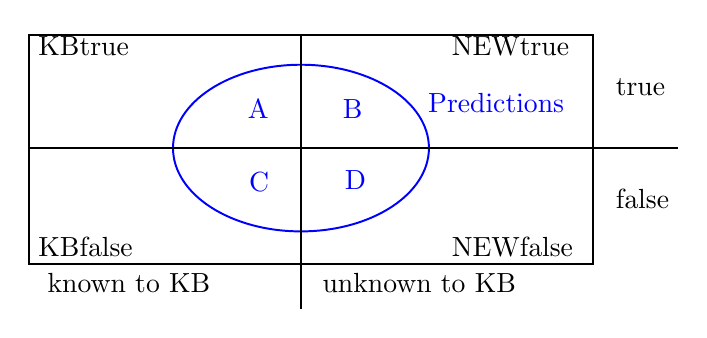
\begin{tikzpicture}

% Fabian: Keep figure in two colors.
% Even if printed in black and white, it's still clear enough

  \path[draw=blue, line width=0.7086614168764338] (3.708333, -1.458333) ellipse (1.625000 and 1.058333);
  \node[above, right, color=blue, font=] at (5.2000, -0.88333) {Predictions};
  \node[above, right, color=blue, font=] at (2.908333, -0.958333) {A};
  \node[above, right, color=blue, font=] at (4.116667, -0.966667) {B};
  \node[above, right, color=blue, font=] at (2.925000, -1.891667) {C};
  \node[above, right, color=blue, font=] at (4.141667, -1.866667) {D};
  \node[above, right, color=black, font=] at (0.250000, -0.166667) {KBtrue};
  \node[above, right, color=black, font=] at (0.250000, -2.708333) {KBfalse};
  \node[above, right, color=black, font=] at (5.500000, -0.166667) {NEWtrue};
  \node[above, right, color=black, font=] at (5.500000, -2.708333) {NEWfalse};
  \node[above, right, color=black, font=] at (7.583333, -0.683333) {true};
  \node[above, right, color=black, font=] at (7.583333, -2.100000) {false};
  \node[above, right, color=black, font=] at (0.366667, -3.166667) {known to KB};
  \node[above, right, color=black, font=] at (3.858333, -3.166667) {unknown to KB};
  \path[draw=black, line width=0.7086614168764338] (0.250000, -0.016667) rectangle (7.416667, -2.933333);
  \draw[draw=black, line width=0.7086614168764338] (0.250000, -1.458333) -- (8.500000, -1.458333);
  \draw[draw=black, line width=0.7086614168764338] (3.708333, -0.025000) -- (3.708333, -3.500000);
\end{tikzpicture}
}

}

\www{
\paragraph{Goal} 
Our goal is to find rules that make true predictions that go beyond the current KB. 
In the figure, we wish to maximize the area B, and to minimize the area D. 
There are two obvious challenges in this context: First, the areas NEWtrue and NEWfalse are unknown. 
So if we wish to maximize B at the expense of D, we are operating in an area outside our KB. 
We would want to use the areas KBtrue and KBfalse to estimate the unknown area. 
This, however, leads to the second challenge: Semantic KBs do not contain negative evidence. 
Thus, the area KBfalse is empty. In the following, we discuss different measures that address these challenges.
}

% \www{
% \paragraph{Support} 
% The \emph{support} of a rule quantifies the number of correct predictions, i.e., the size of A. There are several ways to define the support: It can be the number of instantiations of the rule that appear in the KB. This is what our analogy to association rule mining \cite{AgrImiSwa93} suggests (Section \ref{sec:preliminaries}). This measure, however, is not monotonic if we add atoms to the body. Consider, for example, the rule
% \indented{
%   \emph{marriedTo(}$x,y) \Rightarrow$ \emph{marriedTo(}$y,x$)
% }
% If we add \emph{hasGender($x$,male)} to the body, the number of instantiations that are in the KB decreases. If we add an atom with a fresh variable, e.g., \emph{hasFriend($x$,$z$)}, to the body, the number of instantiations increases for every friend of $x$. This is true even if we add another atom with $z$ to make the rule closed.\
% Alternatively, we can count the number of facts in one particular body atom.
% This definition, however, depends on the choice of the body atom, so that the same rule can have different supports. We can also count the number of facts of the head atom.
% This measure decreases monotonically if more body atoms are added 
% and avoids equivalent rules with different support values. With this in mind, we define the support of a rule as the number of distinct pairs of subjects and objects in the head of all instantiations that appear in the KB:
% \[supp(\vec{B} \Rightarrow r(x,y)) := \#(x,y): \exists z_1,...,z_m: \vec{B} \wedge r(x,y)\]
% where $z_1,...,z_m$ are the variables of the rule apart from $x$ and $y$.
% }

\www{
\paragraph{Support} 
The \emph{support} of a rule quantifies the number of correct predictions, i.e., the size of A. 
There are several ways to define the support: It can be the number of instantiations of the rule that appear in the KB. 
%This is what our analogy to association rule mining \cite{AgrImiSwa93} suggests (Section \ref{sec:preliminaries}). \comment{Katja}{Remove this sentence if the section about association rule mining is removed permanently.}
This measure, however, is not monotonic if we add atoms to the body. Consider, for example, the rule
\indented{
  \emph{marriedTo(}$x,y) \Rightarrow$ \emph{marriedTo(}$y,x$)
}
If we add \emph{hasGender($x$,male)} to the body, the number of instantiations that are in the KB decreases. 
If we add an atom with a fresh variable, e.g., \emph{hasFriend($x$,$z$)}, to the body, the number of instantiations increases for every friend of $x$. 
This is true even if we add another atom with $z$ to obtain a closed rule.\
Alternatively, we can count the number of facts in one particular body atom.
This definition, however, depends on the choice of the body atom, so that the same rule can have different supports. 
We can also count the number of facts of the head atom.
This measure decreases monotonically if more body atoms are added and avoids equivalent rules with different support values. 
With this in mind, we define the support of a rule as the number of distinct pairs of subjects and objects in the head of all instantiations that appear in the KB:
\[supp(\vec{B} \Rightarrow r(x,y)) := \#(x,y): \exists z_1,...,z_m: \vec{B} \wedge r(x,y)\]
where $z_1,...,z_m$ are the variables of the rule apart from $x$ and $y$. }
Note that the support is defined even for rules that are not closed.


% \www{
% \paragraph{Head Coverage} %\comment{check again}
% % Support is an absolute number. This means that a user who thresholds on support has to know the absolute size of the KB to give meaningful values. 
% % To avoid this, we also need to define a proportional version of support, the \emph{head coverage}. It is the proportion of pairs from the head relation that are covered by the predictions of the rule:
% % \[hc(\vec{B} \Rightarrow r(x,y)) := \frac{supp(\vec{B} \Rightarrow r(x,y))}{\#(x,y) : r(x,y)}\]
% Support is an absolute number. This means that a user who thresholds on support has to know the absolute size of the KB to give meaningful values. 
% To avoid this, we also define a proportional version of support. A naive way would be to use the absolute number of support, as defined in the previous paragraph, over the size of the KB. 
% In this case, however, relations that do not have many facts (either because of the incompleteness of the KB or because of their nature), will not be considered in the head of rules,
% i.e. we will not learn rules predicting such relations. Therefore, we propose to use the notion of \emph{head coverage}. 
% This is the proportion of pairs from the head relation that are covered by the predictions of the rule
% % Head coverage is the proportion of pairs from the head relation that are covered by the predictions of the rule:
% \[hc(\vec{B} \Rightarrow r(x,y)) := \frac{supp(\vec{B} \Rightarrow r(x,y))}{\#(x',y') : r(x',y')}\]
% }


\www{
\paragraph{Head Coverage}
Support is an absolute number. This means that a user defining thresholds on support has to know the absolute size of the KB to give meaningful values. 
To avoid this, we propose a proportional version of support. A naive way would be to use the absolute number of support, as defined in the previous paragraph, over the size of the KB. 
In this case, however, relations that do not have many facts (either because of the incompleteness of the KB or because of their nature) will not be considered in the head of the rules,
i.e., we will not learn rules predicting such relations. Therefore, we propose to use the notion of \emph{head coverage}:
\[hc(\vec{B} \Rightarrow r(x,y)) := \frac{supp(\vec{B} \Rightarrow r(x,y))}{size(r)}\]
}

with $size(r) := \#(x',y') : r(x',y')$ denoting the number of facts in relation $r$.

Head coverage quantifies the percentage of the known true facts that are implied %(for the case of closed rules) %or can possibly be implied (for the case of not yet closed rules)
% Fabian: I think that this description is sufficient. The mroe precise one risks confusing readers.
by the rule.
Head coverage can be a measure of statistical significance for any measure used to evaluate the quality of a rule. 
\comment{Fabian}{I am not sure about this. Could you explain? If it is not crucial here, I would omit it at this position.}



\www{
\paragraph{Negative Examples} 
The central challenge of our setting is to provide counter-examples for the rule mining. 
These can take the role of KBfalse, so that we can estimate the areas NEWtrue and NEWfalse. 
There are several approaches to this problem: The standard confidence, the standard positive-only learning evaluation score of ILP, and the partial completeness assumption that we propose. 
}
We will now present these approaches in detail.

% \www{
% \paragraph{Standard Confidence} 
% The standard confidence measure takes all facts that are not in the KB (i.e., NEWtrue and NEWfalse) as negative evidence. 
% Thus, the standard confidence of a rule is the ratio of its predictions that are in the KB, i.e., the share of A in the set of predictions:
% \[conf(\vec{B} \Rightarrow r(x,y)) := \frac{supp(\vec{B} \Rightarrow r(x,y))}{\#(x,y): \exists z_1,...,z_m: \vec{B}}\]
% %\[conf(\vec{B} \Rightarrow r(x,y)) := \frac{supp(\vec{B} \Rightarrow r(x,y))}{supp(\vec{B})}\]
% The standard confidence is blind to the distinction between ``false'' and ``unknown''. Thus, it implements a closed world setting. It mainly describes the known data and penalizes rules that make a large number of predictions in the unknown region. We, in contrast, aim to maximize the number of true predictions that go beyond the current knowledge. We do not want to describe data, but to predict data.
% }



\www{
\paragraph{Standard Confidence} 
The standard confidence measure takes all facts that are not in the KB (i.e., NEWtrue and NEWfalse) as negative evidence. 
Thus, the standard confidence of a rule is the ratio of its predictions that are in the KB, i.e., the share of A (KBtrue) in the set of predictions:
%\[conf(\vec{B} \Rightarrow r(x,y)) := \frac{supp(\vec{B} \Rightarrow r(x,y))}{\#(x,y): \exists z_1,...,z_m: \vec{B}}\]
}

%\comment{Katja}{I prefer the second one.}
\[conf(\vec{B} \Rightarrow r(x,y)) := \frac{\#(x,y): \exists z_1,...,z_m: \vec{B} \wedge r(x,y)}{\#(x,y): \exists z_1,...,z_m: \vec{B}}\]
%\[conf(\vec{B} \Rightarrow r(x,y)) := \frac{supp(\vec{B} \Rightarrow r(x,y))}{supp(\vec{B})}\]

Standard confidence is the measure traditionally used in association rule mining and market basket analysis, where a Closed World Assumption (CWA) is made: 
if there is no evidence in any of the transactions of the database that a user bought a specific product, then this user did not buy the product.
Although natural for the market basket analysis scenario, standard confidence fails to distinguish between ``false'' and ``unknown'' facts, 
which makes it inappropriate for a scenario with Open World semantics, like ours. Moreover, we also persue a different goal than market basket analysis:
we aim to maximize the number of true predictions that go beyond the current knowledge, whereas market basket analysis usually tries to mine rules that can describe data that is already known. 






\www{
\paragraph{Positive-Only Learning} 
For cases where the KB does not contain negative examples, Muggleton has developed a \emph{positive-only learning evaluation score} for ILP \cite{Muggleton:1996:LPD:647996.742465},\cite{usir1753}. 
It takes random facts as negative evidence:
\[
 Score = log(P)-log\frac{R+1}{Rsize+2}-\frac{L}{P}
\]
Here, $P$ is the number of known true facts covered (KBtree, or A resp., in Figure~\ref{fig:prediction}), $R$ is the number of randoms covered, $Rsize$ is the total number of randoms and $L$ is the number of atoms in the hypotheses. 
The intuition is that a good rule should cover many positive examples, and few or no randomly generated examples. This ensures  
that the rule is not overly general. Furthermore, the rule should use as few atoms as possible, and thus achieve a high compression. This measure is implemented (among others) in the ALEPH system.
}


% \www{
% \paragraph{Partial Completeness} 
% We propose to generate negative evidence by the \emph{partial completeness assumption} (PCA).
% This is the assumption that if $r(x,y) \in$ \emph{KBtrue} for some $x,y$, then
% \[\forall y': r(x,y') \in \mbox{\emph{KBtrue}} \cup \mbox{\emph{NEWtrue}} \Rightarrow r(x,y') \in \mbox{\emph{KBtrue}}\] 
% In other words, we assume that if the database knows some $r$-attribute of $x$, then it knows all $r$-attributes of $x$. This assumption is certainly true for functional relations $r$, 
% such as birth dates, capitals, etc. Thanks to the FUN-Property (see Section \ref{sec:model}), it is also true for inverse-functional relations, such as \emph{owns}, \emph{created}, etc. 
% The assumption is also true in the vast majority of cases for relations that are not functional, but that have a high functionality. 
% Even for other relations, the PCA is still reasonable for knowledge bases that have been extracted from a single source (such as DBpedia and YAGO). 
% These usually contain either all $r$-values or none for a given entity.
% }


\paragraph{Partial Completeness} 
We propose to generate negative evidence by means of the \emph{partial completeness assumption} (PCA).
This is the assumption that if $r(x,y) \in$ \emph{KBtrue} for some $x,y$,
%and $x$ is the input variable, 
% Fabian: we already said that all relations are more functional than inverse functional
then
\[\forall y': r(x,y') \in \mbox{\emph{KBtrue}} \cup \mbox{\emph{NEWtrue}} \Rightarrow r(x,y') \in \mbox{\emph{KBtrue}}\] 
%In other words, we assume that if the database knows some $r$-attribute of $x$, then it knows all $r$-attributes of $x$. 
%In other words, we assume that if the database knows some entity for the output variable $y$ for a given relation $r$ and entity of the input variable $x$, 
%then it knows all possible entities for the  output variable $y$ for these $r$ and $x$.
%\comment{Katja}{The term ``$r$-attribute of $x$'' is not intuitive for the reader as it has not been formally introduced, and the term attribute occurs only here. I suggest to replace it.}
% Fabian: I gave it another try, without the input and output:
In other words, we assume that if we know one $y$ for a given $x$, then we know all $y$ for that $x$.

This assumption is certainly true for functional relations $r$, such as \emph{birthdates} and \emph{capitals}.
Thanks to the FUN-property, the assumption is also true for inverse-functional relations, such as \emph{owns} and \emph{created}.
%, with the difference that in this case $x$ is the output variable and $y$ the input variable.
%, with the difference that in this case we assume that we know all $r$-attributes of $y$ (since $y$ is the input variable in this case).
The assumption is also true in the vast majority of cases for relations that are not functional, but that have a high functionality. 
Even for other relations, the PCA is still reasonable for knowledge bases that have been extracted from a single source (such as DBpedia and YAGO), as we shall see. 
%These usually contain either all $r$-values or none for a given entity. \comment{Katja}{Likewise, the term ``$r$-values'' is not introduced.}
We present an experimental evaluation of the PCA in Section~\ref{sec:experimentsPCA}.

% \www{
% \paragraph{PCA Confidence} 
% Under the PCA, we normalize the confidence not by the entire set of facts, but by the set of facts of which we know that they are true, together with the facts of which we assume that they are false. If the head atom of the rule is $r(x,y)$, then this set is just the set of facts $\{ r(x,y') : r(x,y') \in \mathcal{K}\}$. Thanks to the FUN-Property, the PCA is always applied to the first argument of the head atom:
% %\[pcaconf(\vec{B} \Rightarrow r(x,y)) := \frac{\#(x,y): \exists z_1,...,z_m: \vec{B} \wedge r(x,y)}{\#(x,y): \exists z_1,...,z_m,y': \vec{B} \wedge r(x,y')}\]
% \[pcaconf(\vec{B} \Rightarrow r(x,y)) := \frac{supp(\vec{B} \Rightarrow r(x,y))}{\#(x,y): \exists z_1,...,z_m,y': \vec{B} \wedge r(x,y')}\]
% We show in our experiments that the PCA confidence identifies much more productive rules than the other measures.
% }



\paragraph{PCA Confidence} 
\label{pcaConf}
Under the PCA, the denominator of the confidence will not be the size of the entire set of facts that the body of the rule produces, 
but the number of facts that we know to be true together with the facts that we assume to be false. 
\comment{Fabian}{Important fix here: Christina found that the denominator should count $\#(x,y)$, and not $\#(x,y')$.}

% If the head atom of the rule is $r(x,y)$, then this set is just the set of facts $\{ r(x,y') : r(x,y') \in \mathcal{K}\}$. 
% The PCA confidence for a rule with $x$ as the input variable is defined as:
% \[
% \small \hspace*{-1ex}
% conf_{PCA}(\vec{B} \Rightarrow r(x,y)) := \frac{supp(\vec{B} \Rightarrow r(x,y))}{\#(x,y): \exists z_1,...,z_m,y': \vec{B} \wedge r(x,y')}
% \]
% \comment{Katja}{If we replace the formula for the standard confidence, we should use the same notation here:
\[
\small \hspace*{-2ex}
conf_{PCA}(\vec{B} \Rightarrow r(x,y)) := \frac{\#(x,y): \exists z_1,...,z_m: \vec{B} \wedge r(x,y)}{\#(x,y): \exists z_1,...,z_m,y': \vec{B} \wedge r(x,y')}
\]
%}
This confidence normalizes the support by the number of pairs $(x,y)$ for which there exists a $y'$ with $r(x,y')$, i.e., for which we assume that the KB knows all such $y'$.
\comment{Chris}{Think about if you want to include the following one.} 
\comment{Katja}{I suggest to remove it because we will have a detailed discussion in the experiments and do not need it already here.}
The PCA confidence can be seen as a process in which we first take a biased sample of the body (those facts containing entities for the $x$ variable that appear also in the head)
and then calculate the standard confidence over this sample. 
The fact that our sample is biased implies that PCA confidence might not be a good estimator of the actual predictive power of the rule (precision).
However, our experiments show that overall PCA confidence identifies much more productive rules than the other measures and it also correlates with precision better than the standard confidence.

%- - - - - - - - - - - - - - - - - - - - - - - - - - - - - -
\section{Confidence Measures}
\label{sec:pca}
% !TEX root = main.tex

%\paragraph{PCA Assumption}
\label{sec:experimentsPCA}

\comment{R3}{I would like to understand sooner that 4.3 is a discarded and useless digression and I would appreciate a deeper discussion of Section 4.4, 
possibly with examples (note that 4.4 and 4.4.2 have the same title, which is not elegant)}

\comment{Chris}{Removed PosOnly evaluation function, merged PCA assumption-PCA confidence. Discussed by example of table 1. Removed the FUN-property stuff}



The support of a rule quantifies the number of known correct predictions of the rule. 
However, it does not take into account the false predictions of the rule.
We will now describe measures that judge the rule \emph{quality}.
We first describe the challenges in defining such a measure in our setting 
and discuss the most common way to measure the rule quality which we refer to as standard confidence.
Then, we introduce our own measure: the confidence under the assumption of partial completeness.



% The support of a rule quantifies the number of known correct predictions of the rule. However, it does not measure the false predictions of the rule.
% We will now describe measures that judge the rule \emph{quality}.
% We first describe the challenges in defining such a measure in our setting %of our setting w.r.t. designing a good measure for judging the quality of a rule,
% and discuss existing measures: the standard confidence and the Positive-Only Learning score.
% Then, we introduce our own measure: the confidence under the assumption of partial completeness.
% We also discuss the practical applicability of this assumption.

\subsection{Challenges}
Let us consider a given Horn rule $\vec{B} \Rightarrow r(x,y)$. Let us look at all facts with relation $r$ (Figure \ref{fig:prediction}).
We distinguish 4 types of facts: True facts that are known to the KB (KBtrue), true facts that are unknown to the KB (NEWtrue),
facts that are known to be false in the KB (KBfalse), and facts that are false but unknown to the KB (NEWfalse).
The rule will make certain predictions about relation $r$ (blue circle). These predictions can be known to be true (A), known to be false (C), or unknown (B and D).
When they are unknown to the KB, they can still be true (B) or false (D) with respect to the real world.\\

%\ffigure{Figure}{model}{\label{fig:prediction}Prediction under Incompleteness}{% This is the TIKZ version of the file
%     model.svg
% generated by PowerLine, the free SVG editor with Latex support

% To include this picture in LaTex, write the following in its preamble:
%  \usepackage{tikz}
%  \usepackage{graphicx}
%  \usepackage{hyperref}
% Then write '% !TEX root = main.tex

\www{
\paragraph{Model} We follow the description of the mining model from \cite{amie}.
Let us consider a given Horn rule $\vec{B} \Rightarrow r(x,y)$. Let us look at all facts with relation $r$ (Figure \ref{model}). 
We distinguish 4 types of facts: True facts that are known to the KB (KBtrue), true facts that are unknown to the KB (NEWtrue), 
facts that are known to be false in the KB (KBfalse), and facts that are false but unknown to the KB (NEWfalse). 
The rule will make certain predictions (blue circle). These predictions can be known to be true (A), known to be false (C), or unknown (B and D). 
When they are unknown to the KB, they can still be true (B) or false (D) with respect to the real world.\\

\ffigure{Figure}{model}{\label{fig:prediction}Prediction under Incompleteness}{\input{figures/modelpic.tikz}}

}

\www{
\paragraph{Goal} 
Our goal is to find rules that make true predictions that go beyond the current KB. 
In the figure, we wish to maximize the area B, and to minimize the area D. 
There are two obvious challenges in this context: First, the areas NEWtrue and NEWfalse are unknown. 
So if we wish to maximize B at the expense of D, we are operating in an area outside our KB. 
We would want to use the areas KBtrue and KBfalse to estimate the unknown area. 
This, however, leads to the second challenge: Semantic KBs do not contain negative evidence. 
Thus, the area KBfalse is empty. In the following, we discuss different measures that address these challenges.
}

% \www{
% \paragraph{Support} 
% The \emph{support} of a rule quantifies the number of correct predictions, i.e., the size of A. There are several ways to define the support: It can be the number of instantiations of the rule that appear in the KB. This is what our analogy to association rule mining \cite{AgrImiSwa93} suggests (Section \ref{sec:preliminaries}). This measure, however, is not monotonic if we add atoms to the body. Consider, for example, the rule
% \indented{
%   \emph{marriedTo(}$x,y) \Rightarrow$ \emph{marriedTo(}$y,x$)
% }
% If we add \emph{hasGender($x$,male)} to the body, the number of instantiations that are in the KB decreases. If we add an atom with a fresh variable, e.g., \emph{hasFriend($x$,$z$)}, to the body, the number of instantiations increases for every friend of $x$. This is true even if we add another atom with $z$ to make the rule closed.\
% Alternatively, we can count the number of facts in one particular body atom.
% This definition, however, depends on the choice of the body atom, so that the same rule can have different supports. We can also count the number of facts of the head atom.
% This measure decreases monotonically if more body atoms are added 
% and avoids equivalent rules with different support values. With this in mind, we define the support of a rule as the number of distinct pairs of subjects and objects in the head of all instantiations that appear in the KB:
% \[supp(\vec{B} \Rightarrow r(x,y)) := \#(x,y): \exists z_1,...,z_m: \vec{B} \wedge r(x,y)\]
% where $z_1,...,z_m$ are the variables of the rule apart from $x$ and $y$.
% }

\www{
\paragraph{Support} 
The \emph{support} of a rule quantifies the number of correct predictions, i.e., the size of A. 
There are several ways to define the support: It can be the number of instantiations of the rule that appear in the KB. 
%This is what our analogy to association rule mining \cite{AgrImiSwa93} suggests (Section \ref{sec:preliminaries}). \comment{Katja}{Remove this sentence if the section about association rule mining is removed permanently.}
This measure, however, is not monotonic if we add atoms to the body. Consider, for example, the rule
\indented{
  \emph{marriedTo(}$x,y) \Rightarrow$ \emph{marriedTo(}$y,x$)
}
If we add \emph{hasGender($x$,male)} to the body, the number of instantiations that are in the KB decreases. 
If we add an atom with a fresh variable, e.g., \emph{hasFriend($x$,$z$)}, to the body, the number of instantiations increases for every friend of $x$. 
This is true even if we add another atom with $z$ to obtain a closed rule.\
Alternatively, we can count the number of facts in one particular body atom.
This definition, however, depends on the choice of the body atom, so that the same rule can have different supports. 
We can also count the number of facts of the head atom.
This measure decreases monotonically if more body atoms are added and avoids equivalent rules with different support values. 
With this in mind, we define the support of a rule as the number of distinct pairs of subjects and objects in the head of all instantiations that appear in the KB:
\[supp(\vec{B} \Rightarrow r(x,y)) := \#(x,y): \exists z_1,...,z_m: \vec{B} \wedge r(x,y)\]
where $z_1,...,z_m$ are the variables of the rule apart from $x$ and $y$. }
Note that the support is defined even for rules that are not closed.


% \www{
% \paragraph{Head Coverage} %\comment{check again}
% % Support is an absolute number. This means that a user who thresholds on support has to know the absolute size of the KB to give meaningful values. 
% % To avoid this, we also need to define a proportional version of support, the \emph{head coverage}. It is the proportion of pairs from the head relation that are covered by the predictions of the rule:
% % \[hc(\vec{B} \Rightarrow r(x,y)) := \frac{supp(\vec{B} \Rightarrow r(x,y))}{\#(x,y) : r(x,y)}\]
% Support is an absolute number. This means that a user who thresholds on support has to know the absolute size of the KB to give meaningful values. 
% To avoid this, we also define a proportional version of support. A naive way would be to use the absolute number of support, as defined in the previous paragraph, over the size of the KB. 
% In this case, however, relations that do not have many facts (either because of the incompleteness of the KB or because of their nature), will not be considered in the head of rules,
% i.e. we will not learn rules predicting such relations. Therefore, we propose to use the notion of \emph{head coverage}. 
% This is the proportion of pairs from the head relation that are covered by the predictions of the rule
% % Head coverage is the proportion of pairs from the head relation that are covered by the predictions of the rule:
% \[hc(\vec{B} \Rightarrow r(x,y)) := \frac{supp(\vec{B} \Rightarrow r(x,y))}{\#(x',y') : r(x',y')}\]
% }


\www{
\paragraph{Head Coverage}
Support is an absolute number. This means that a user defining thresholds on support has to know the absolute size of the KB to give meaningful values. 
To avoid this, we propose a proportional version of support. A naive way would be to use the absolute number of support, as defined in the previous paragraph, over the size of the KB. 
In this case, however, relations that do not have many facts (either because of the incompleteness of the KB or because of their nature) will not be considered in the head of the rules,
i.e., we will not learn rules predicting such relations. Therefore, we propose to use the notion of \emph{head coverage}:
\[hc(\vec{B} \Rightarrow r(x,y)) := \frac{supp(\vec{B} \Rightarrow r(x,y))}{size(r)}\]
}

with $size(r) := \#(x',y') : r(x',y')$ denoting the number of facts in relation $r$.

Head coverage quantifies the percentage of the known true facts that are implied %(for the case of closed rules) %or can possibly be implied (for the case of not yet closed rules)
% Fabian: I think that this description is sufficient. The mroe precise one risks confusing readers.
by the rule.
Head coverage can be a measure of statistical significance for any measure used to evaluate the quality of a rule. 
\comment{Fabian}{I am not sure about this. Could you explain? If it is not crucial here, I would omit it at this position.}



\www{
\paragraph{Negative Examples} 
The central challenge of our setting is to provide counter-examples for the rule mining. 
These can take the role of KBfalse, so that we can estimate the areas NEWtrue and NEWfalse. 
There are several approaches to this problem: The standard confidence, the standard positive-only learning evaluation score of ILP, and the partial completeness assumption that we propose. 
}
We will now present these approaches in detail.

% \www{
% \paragraph{Standard Confidence} 
% The standard confidence measure takes all facts that are not in the KB (i.e., NEWtrue and NEWfalse) as negative evidence. 
% Thus, the standard confidence of a rule is the ratio of its predictions that are in the KB, i.e., the share of A in the set of predictions:
% \[conf(\vec{B} \Rightarrow r(x,y)) := \frac{supp(\vec{B} \Rightarrow r(x,y))}{\#(x,y): \exists z_1,...,z_m: \vec{B}}\]
% %\[conf(\vec{B} \Rightarrow r(x,y)) := \frac{supp(\vec{B} \Rightarrow r(x,y))}{supp(\vec{B})}\]
% The standard confidence is blind to the distinction between ``false'' and ``unknown''. Thus, it implements a closed world setting. It mainly describes the known data and penalizes rules that make a large number of predictions in the unknown region. We, in contrast, aim to maximize the number of true predictions that go beyond the current knowledge. We do not want to describe data, but to predict data.
% }



\www{
\paragraph{Standard Confidence} 
The standard confidence measure takes all facts that are not in the KB (i.e., NEWtrue and NEWfalse) as negative evidence. 
Thus, the standard confidence of a rule is the ratio of its predictions that are in the KB, i.e., the share of A (KBtrue) in the set of predictions:
%\[conf(\vec{B} \Rightarrow r(x,y)) := \frac{supp(\vec{B} \Rightarrow r(x,y))}{\#(x,y): \exists z_1,...,z_m: \vec{B}}\]
}

%\comment{Katja}{I prefer the second one.}
\[conf(\vec{B} \Rightarrow r(x,y)) := \frac{\#(x,y): \exists z_1,...,z_m: \vec{B} \wedge r(x,y)}{\#(x,y): \exists z_1,...,z_m: \vec{B}}\]
%\[conf(\vec{B} \Rightarrow r(x,y)) := \frac{supp(\vec{B} \Rightarrow r(x,y))}{supp(\vec{B})}\]

Standard confidence is the measure traditionally used in association rule mining and market basket analysis, where a Closed World Assumption (CWA) is made: 
if there is no evidence in any of the transactions of the database that a user bought a specific product, then this user did not buy the product.
Although natural for the market basket analysis scenario, standard confidence fails to distinguish between ``false'' and ``unknown'' facts, 
which makes it inappropriate for a scenario with Open World semantics, like ours. Moreover, we also persue a different goal than market basket analysis:
we aim to maximize the number of true predictions that go beyond the current knowledge, whereas market basket analysis usually tries to mine rules that can describe data that is already known. 






\www{
\paragraph{Positive-Only Learning} 
For cases where the KB does not contain negative examples, Muggleton has developed a \emph{positive-only learning evaluation score} for ILP \cite{Muggleton:1996:LPD:647996.742465},\cite{usir1753}. 
It takes random facts as negative evidence:
\[
 Score = log(P)-log\frac{R+1}{Rsize+2}-\frac{L}{P}
\]
Here, $P$ is the number of known true facts covered (KBtree, or A resp., in Figure~\ref{fig:prediction}), $R$ is the number of randoms covered, $Rsize$ is the total number of randoms and $L$ is the number of atoms in the hypotheses. 
The intuition is that a good rule should cover many positive examples, and few or no randomly generated examples. This ensures  
that the rule is not overly general. Furthermore, the rule should use as few atoms as possible, and thus achieve a high compression. This measure is implemented (among others) in the ALEPH system.
}


% \www{
% \paragraph{Partial Completeness} 
% We propose to generate negative evidence by the \emph{partial completeness assumption} (PCA).
% This is the assumption that if $r(x,y) \in$ \emph{KBtrue} for some $x,y$, then
% \[\forall y': r(x,y') \in \mbox{\emph{KBtrue}} \cup \mbox{\emph{NEWtrue}} \Rightarrow r(x,y') \in \mbox{\emph{KBtrue}}\] 
% In other words, we assume that if the database knows some $r$-attribute of $x$, then it knows all $r$-attributes of $x$. This assumption is certainly true for functional relations $r$, 
% such as birth dates, capitals, etc. Thanks to the FUN-Property (see Section \ref{sec:model}), it is also true for inverse-functional relations, such as \emph{owns}, \emph{created}, etc. 
% The assumption is also true in the vast majority of cases for relations that are not functional, but that have a high functionality. 
% Even for other relations, the PCA is still reasonable for knowledge bases that have been extracted from a single source (such as DBpedia and YAGO). 
% These usually contain either all $r$-values or none for a given entity.
% }


\paragraph{Partial Completeness} 
We propose to generate negative evidence by means of the \emph{partial completeness assumption} (PCA).
This is the assumption that if $r(x,y) \in$ \emph{KBtrue} for some $x,y$,
%and $x$ is the input variable, 
% Fabian: we already said that all relations are more functional than inverse functional
then
\[\forall y': r(x,y') \in \mbox{\emph{KBtrue}} \cup \mbox{\emph{NEWtrue}} \Rightarrow r(x,y') \in \mbox{\emph{KBtrue}}\] 
%In other words, we assume that if the database knows some $r$-attribute of $x$, then it knows all $r$-attributes of $x$. 
%In other words, we assume that if the database knows some entity for the output variable $y$ for a given relation $r$ and entity of the input variable $x$, 
%then it knows all possible entities for the  output variable $y$ for these $r$ and $x$.
%\comment{Katja}{The term ``$r$-attribute of $x$'' is not intuitive for the reader as it has not been formally introduced, and the term attribute occurs only here. I suggest to replace it.}
% Fabian: I gave it another try, without the input and output:
In other words, we assume that if we know one $y$ for a given $x$, then we know all $y$ for that $x$.

This assumption is certainly true for functional relations $r$, such as \emph{birthdates} and \emph{capitals}.
Thanks to the FUN-property, the assumption is also true for inverse-functional relations, such as \emph{owns} and \emph{created}.
%, with the difference that in this case $x$ is the output variable and $y$ the input variable.
%, with the difference that in this case we assume that we know all $r$-attributes of $y$ (since $y$ is the input variable in this case).
The assumption is also true in the vast majority of cases for relations that are not functional, but that have a high functionality. 
Even for other relations, the PCA is still reasonable for knowledge bases that have been extracted from a single source (such as DBpedia and YAGO), as we shall see. 
%These usually contain either all $r$-values or none for a given entity. \comment{Katja}{Likewise, the term ``$r$-values'' is not introduced.}
We present an experimental evaluation of the PCA in Section~\ref{sec:experimentsPCA}.

% \www{
% \paragraph{PCA Confidence} 
% Under the PCA, we normalize the confidence not by the entire set of facts, but by the set of facts of which we know that they are true, together with the facts of which we assume that they are false. If the head atom of the rule is $r(x,y)$, then this set is just the set of facts $\{ r(x,y') : r(x,y') \in \mathcal{K}\}$. Thanks to the FUN-Property, the PCA is always applied to the first argument of the head atom:
% %\[pcaconf(\vec{B} \Rightarrow r(x,y)) := \frac{\#(x,y): \exists z_1,...,z_m: \vec{B} \wedge r(x,y)}{\#(x,y): \exists z_1,...,z_m,y': \vec{B} \wedge r(x,y')}\]
% \[pcaconf(\vec{B} \Rightarrow r(x,y)) := \frac{supp(\vec{B} \Rightarrow r(x,y))}{\#(x,y): \exists z_1,...,z_m,y': \vec{B} \wedge r(x,y')}\]
% We show in our experiments that the PCA confidence identifies much more productive rules than the other measures.
% }



\paragraph{PCA Confidence} 
\label{pcaConf}
Under the PCA, the denominator of the confidence will not be the size of the entire set of facts that the body of the rule produces, 
but the number of facts that we know to be true together with the facts that we assume to be false. 
\comment{Fabian}{Important fix here: Christina found that the denominator should count $\#(x,y)$, and not $\#(x,y')$.}

% If the head atom of the rule is $r(x,y)$, then this set is just the set of facts $\{ r(x,y') : r(x,y') \in \mathcal{K}\}$. 
% The PCA confidence for a rule with $x$ as the input variable is defined as:
% \[
% \small \hspace*{-1ex}
% conf_{PCA}(\vec{B} \Rightarrow r(x,y)) := \frac{supp(\vec{B} \Rightarrow r(x,y))}{\#(x,y): \exists z_1,...,z_m,y': \vec{B} \wedge r(x,y')}
% \]
% \comment{Katja}{If we replace the formula for the standard confidence, we should use the same notation here:
\[
\small \hspace*{-2ex}
conf_{PCA}(\vec{B} \Rightarrow r(x,y)) := \frac{\#(x,y): \exists z_1,...,z_m: \vec{B} \wedge r(x,y)}{\#(x,y): \exists z_1,...,z_m,y': \vec{B} \wedge r(x,y')}
\]
%}
This confidence normalizes the support by the number of pairs $(x,y)$ for which there exists a $y'$ with $r(x,y')$, i.e., for which we assume that the KB knows all such $y'$.
\comment{Chris}{Think about if you want to include the following one.} 
\comment{Katja}{I suggest to remove it because we will have a detailed discussion in the experiments and do not need it already here.}
The PCA confidence can be seen as a process in which we first take a biased sample of the body (those facts containing entities for the $x$ variable that appear also in the head)
and then calculate the standard confidence over this sample. 
The fact that our sample is biased implies that PCA confidence might not be a good estimator of the actual predictive power of the rule (precision).
However, our experiments show that overall PCA confidence identifies much more productive rules than the other measures and it also correlates with precision better than the standard confidence.' where the picture shall appear in the LaTex document.

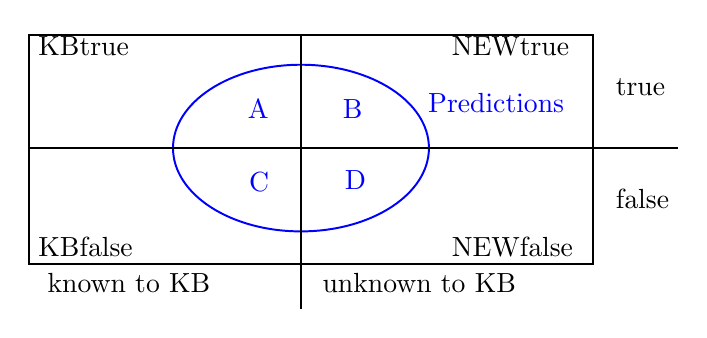
\begin{tikzpicture}

% Fabian: Keep figure in two colors.
% Even if printed in black and white, it's still clear enough

  \path[draw=blue, line width=0.7086614168764338] (3.708333, -1.458333) ellipse (1.625000 and 1.058333);
  \node[above, right, color=blue, font=] at (5.2000, -0.88333) {Predictions};
  \node[above, right, color=blue, font=] at (2.908333, -0.958333) {A};
  \node[above, right, color=blue, font=] at (4.116667, -0.966667) {B};
  \node[above, right, color=blue, font=] at (2.925000, -1.891667) {C};
  \node[above, right, color=blue, font=] at (4.141667, -1.866667) {D};
  \node[above, right, color=black, font=] at (0.250000, -0.166667) {KBtrue};
  \node[above, right, color=black, font=] at (0.250000, -2.708333) {KBfalse};
  \node[above, right, color=black, font=] at (5.500000, -0.166667) {NEWtrue};
  \node[above, right, color=black, font=] at (5.500000, -2.708333) {NEWfalse};
  \node[above, right, color=black, font=] at (7.583333, -0.683333) {true};
  \node[above, right, color=black, font=] at (7.583333, -2.100000) {false};
  \node[above, right, color=black, font=] at (0.366667, -3.166667) {known to KB};
  \node[above, right, color=black, font=] at (3.858333, -3.166667) {unknown to KB};
  \path[draw=black, line width=0.7086614168764338] (0.250000, -0.016667) rectangle (7.416667, -2.933333);
  \draw[draw=black, line width=0.7086614168764338] (0.250000, -1.458333) -- (8.500000, -1.458333);
  \draw[draw=black, line width=0.7086614168764338] (3.708333, -0.025000) -- (3.708333, -3.500000);
\end{tikzpicture}
}
\begin{figure}[h]
\caption{Prediction under Incompleteness}
% This is the TIKZ version of the file
%     model.svg
% generated by PowerLine, the free SVG editor with Latex support

% To include this picture in LaTex, write the following in its preamble:
%  \usepackage{tikz}
%  \usepackage{graphicx}
%  \usepackage{hyperref}
% Then write '% !TEX root = main.tex

\www{
\paragraph{Model} We follow the description of the mining model from \cite{amie}.
Let us consider a given Horn rule $\vec{B} \Rightarrow r(x,y)$. Let us look at all facts with relation $r$ (Figure \ref{model}). 
We distinguish 4 types of facts: True facts that are known to the KB (KBtrue), true facts that are unknown to the KB (NEWtrue), 
facts that are known to be false in the KB (KBfalse), and facts that are false but unknown to the KB (NEWfalse). 
The rule will make certain predictions (blue circle). These predictions can be known to be true (A), known to be false (C), or unknown (B and D). 
When they are unknown to the KB, they can still be true (B) or false (D) with respect to the real world.\\

\ffigure{Figure}{model}{\label{fig:prediction}Prediction under Incompleteness}{\input{figures/modelpic.tikz}}

}

\www{
\paragraph{Goal} 
Our goal is to find rules that make true predictions that go beyond the current KB. 
In the figure, we wish to maximize the area B, and to minimize the area D. 
There are two obvious challenges in this context: First, the areas NEWtrue and NEWfalse are unknown. 
So if we wish to maximize B at the expense of D, we are operating in an area outside our KB. 
We would want to use the areas KBtrue and KBfalse to estimate the unknown area. 
This, however, leads to the second challenge: Semantic KBs do not contain negative evidence. 
Thus, the area KBfalse is empty. In the following, we discuss different measures that address these challenges.
}

% \www{
% \paragraph{Support} 
% The \emph{support} of a rule quantifies the number of correct predictions, i.e., the size of A. There are several ways to define the support: It can be the number of instantiations of the rule that appear in the KB. This is what our analogy to association rule mining \cite{AgrImiSwa93} suggests (Section \ref{sec:preliminaries}). This measure, however, is not monotonic if we add atoms to the body. Consider, for example, the rule
% \indented{
%   \emph{marriedTo(}$x,y) \Rightarrow$ \emph{marriedTo(}$y,x$)
% }
% If we add \emph{hasGender($x$,male)} to the body, the number of instantiations that are in the KB decreases. If we add an atom with a fresh variable, e.g., \emph{hasFriend($x$,$z$)}, to the body, the number of instantiations increases for every friend of $x$. This is true even if we add another atom with $z$ to make the rule closed.\
% Alternatively, we can count the number of facts in one particular body atom.
% This definition, however, depends on the choice of the body atom, so that the same rule can have different supports. We can also count the number of facts of the head atom.
% This measure decreases monotonically if more body atoms are added 
% and avoids equivalent rules with different support values. With this in mind, we define the support of a rule as the number of distinct pairs of subjects and objects in the head of all instantiations that appear in the KB:
% \[supp(\vec{B} \Rightarrow r(x,y)) := \#(x,y): \exists z_1,...,z_m: \vec{B} \wedge r(x,y)\]
% where $z_1,...,z_m$ are the variables of the rule apart from $x$ and $y$.
% }

\www{
\paragraph{Support} 
The \emph{support} of a rule quantifies the number of correct predictions, i.e., the size of A. 
There are several ways to define the support: It can be the number of instantiations of the rule that appear in the KB. 
%This is what our analogy to association rule mining \cite{AgrImiSwa93} suggests (Section \ref{sec:preliminaries}). \comment{Katja}{Remove this sentence if the section about association rule mining is removed permanently.}
This measure, however, is not monotonic if we add atoms to the body. Consider, for example, the rule
\indented{
  \emph{marriedTo(}$x,y) \Rightarrow$ \emph{marriedTo(}$y,x$)
}
If we add \emph{hasGender($x$,male)} to the body, the number of instantiations that are in the KB decreases. 
If we add an atom with a fresh variable, e.g., \emph{hasFriend($x$,$z$)}, to the body, the number of instantiations increases for every friend of $x$. 
This is true even if we add another atom with $z$ to obtain a closed rule.\
Alternatively, we can count the number of facts in one particular body atom.
This definition, however, depends on the choice of the body atom, so that the same rule can have different supports. 
We can also count the number of facts of the head atom.
This measure decreases monotonically if more body atoms are added and avoids equivalent rules with different support values. 
With this in mind, we define the support of a rule as the number of distinct pairs of subjects and objects in the head of all instantiations that appear in the KB:
\[supp(\vec{B} \Rightarrow r(x,y)) := \#(x,y): \exists z_1,...,z_m: \vec{B} \wedge r(x,y)\]
where $z_1,...,z_m$ are the variables of the rule apart from $x$ and $y$. }
Note that the support is defined even for rules that are not closed.


% \www{
% \paragraph{Head Coverage} %\comment{check again}
% % Support is an absolute number. This means that a user who thresholds on support has to know the absolute size of the KB to give meaningful values. 
% % To avoid this, we also need to define a proportional version of support, the \emph{head coverage}. It is the proportion of pairs from the head relation that are covered by the predictions of the rule:
% % \[hc(\vec{B} \Rightarrow r(x,y)) := \frac{supp(\vec{B} \Rightarrow r(x,y))}{\#(x,y) : r(x,y)}\]
% Support is an absolute number. This means that a user who thresholds on support has to know the absolute size of the KB to give meaningful values. 
% To avoid this, we also define a proportional version of support. A naive way would be to use the absolute number of support, as defined in the previous paragraph, over the size of the KB. 
% In this case, however, relations that do not have many facts (either because of the incompleteness of the KB or because of their nature), will not be considered in the head of rules,
% i.e. we will not learn rules predicting such relations. Therefore, we propose to use the notion of \emph{head coverage}. 
% This is the proportion of pairs from the head relation that are covered by the predictions of the rule
% % Head coverage is the proportion of pairs from the head relation that are covered by the predictions of the rule:
% \[hc(\vec{B} \Rightarrow r(x,y)) := \frac{supp(\vec{B} \Rightarrow r(x,y))}{\#(x',y') : r(x',y')}\]
% }


\www{
\paragraph{Head Coverage}
Support is an absolute number. This means that a user defining thresholds on support has to know the absolute size of the KB to give meaningful values. 
To avoid this, we propose a proportional version of support. A naive way would be to use the absolute number of support, as defined in the previous paragraph, over the size of the KB. 
In this case, however, relations that do not have many facts (either because of the incompleteness of the KB or because of their nature) will not be considered in the head of the rules,
i.e., we will not learn rules predicting such relations. Therefore, we propose to use the notion of \emph{head coverage}:
\[hc(\vec{B} \Rightarrow r(x,y)) := \frac{supp(\vec{B} \Rightarrow r(x,y))}{size(r)}\]
}

with $size(r) := \#(x',y') : r(x',y')$ denoting the number of facts in relation $r$.

Head coverage quantifies the percentage of the known true facts that are implied %(for the case of closed rules) %or can possibly be implied (for the case of not yet closed rules)
% Fabian: I think that this description is sufficient. The mroe precise one risks confusing readers.
by the rule.
Head coverage can be a measure of statistical significance for any measure used to evaluate the quality of a rule. 
\comment{Fabian}{I am not sure about this. Could you explain? If it is not crucial here, I would omit it at this position.}



\www{
\paragraph{Negative Examples} 
The central challenge of our setting is to provide counter-examples for the rule mining. 
These can take the role of KBfalse, so that we can estimate the areas NEWtrue and NEWfalse. 
There are several approaches to this problem: The standard confidence, the standard positive-only learning evaluation score of ILP, and the partial completeness assumption that we propose. 
}
We will now present these approaches in detail.

% \www{
% \paragraph{Standard Confidence} 
% The standard confidence measure takes all facts that are not in the KB (i.e., NEWtrue and NEWfalse) as negative evidence. 
% Thus, the standard confidence of a rule is the ratio of its predictions that are in the KB, i.e., the share of A in the set of predictions:
% \[conf(\vec{B} \Rightarrow r(x,y)) := \frac{supp(\vec{B} \Rightarrow r(x,y))}{\#(x,y): \exists z_1,...,z_m: \vec{B}}\]
% %\[conf(\vec{B} \Rightarrow r(x,y)) := \frac{supp(\vec{B} \Rightarrow r(x,y))}{supp(\vec{B})}\]
% The standard confidence is blind to the distinction between ``false'' and ``unknown''. Thus, it implements a closed world setting. It mainly describes the known data and penalizes rules that make a large number of predictions in the unknown region. We, in contrast, aim to maximize the number of true predictions that go beyond the current knowledge. We do not want to describe data, but to predict data.
% }



\www{
\paragraph{Standard Confidence} 
The standard confidence measure takes all facts that are not in the KB (i.e., NEWtrue and NEWfalse) as negative evidence. 
Thus, the standard confidence of a rule is the ratio of its predictions that are in the KB, i.e., the share of A (KBtrue) in the set of predictions:
%\[conf(\vec{B} \Rightarrow r(x,y)) := \frac{supp(\vec{B} \Rightarrow r(x,y))}{\#(x,y): \exists z_1,...,z_m: \vec{B}}\]
}

%\comment{Katja}{I prefer the second one.}
\[conf(\vec{B} \Rightarrow r(x,y)) := \frac{\#(x,y): \exists z_1,...,z_m: \vec{B} \wedge r(x,y)}{\#(x,y): \exists z_1,...,z_m: \vec{B}}\]
%\[conf(\vec{B} \Rightarrow r(x,y)) := \frac{supp(\vec{B} \Rightarrow r(x,y))}{supp(\vec{B})}\]

Standard confidence is the measure traditionally used in association rule mining and market basket analysis, where a Closed World Assumption (CWA) is made: 
if there is no evidence in any of the transactions of the database that a user bought a specific product, then this user did not buy the product.
Although natural for the market basket analysis scenario, standard confidence fails to distinguish between ``false'' and ``unknown'' facts, 
which makes it inappropriate for a scenario with Open World semantics, like ours. Moreover, we also persue a different goal than market basket analysis:
we aim to maximize the number of true predictions that go beyond the current knowledge, whereas market basket analysis usually tries to mine rules that can describe data that is already known. 






\www{
\paragraph{Positive-Only Learning} 
For cases where the KB does not contain negative examples, Muggleton has developed a \emph{positive-only learning evaluation score} for ILP \cite{Muggleton:1996:LPD:647996.742465},\cite{usir1753}. 
It takes random facts as negative evidence:
\[
 Score = log(P)-log\frac{R+1}{Rsize+2}-\frac{L}{P}
\]
Here, $P$ is the number of known true facts covered (KBtree, or A resp., in Figure~\ref{fig:prediction}), $R$ is the number of randoms covered, $Rsize$ is the total number of randoms and $L$ is the number of atoms in the hypotheses. 
The intuition is that a good rule should cover many positive examples, and few or no randomly generated examples. This ensures  
that the rule is not overly general. Furthermore, the rule should use as few atoms as possible, and thus achieve a high compression. This measure is implemented (among others) in the ALEPH system.
}


% \www{
% \paragraph{Partial Completeness} 
% We propose to generate negative evidence by the \emph{partial completeness assumption} (PCA).
% This is the assumption that if $r(x,y) \in$ \emph{KBtrue} for some $x,y$, then
% \[\forall y': r(x,y') \in \mbox{\emph{KBtrue}} \cup \mbox{\emph{NEWtrue}} \Rightarrow r(x,y') \in \mbox{\emph{KBtrue}}\] 
% In other words, we assume that if the database knows some $r$-attribute of $x$, then it knows all $r$-attributes of $x$. This assumption is certainly true for functional relations $r$, 
% such as birth dates, capitals, etc. Thanks to the FUN-Property (see Section \ref{sec:model}), it is also true for inverse-functional relations, such as \emph{owns}, \emph{created}, etc. 
% The assumption is also true in the vast majority of cases for relations that are not functional, but that have a high functionality. 
% Even for other relations, the PCA is still reasonable for knowledge bases that have been extracted from a single source (such as DBpedia and YAGO). 
% These usually contain either all $r$-values or none for a given entity.
% }


\paragraph{Partial Completeness} 
We propose to generate negative evidence by means of the \emph{partial completeness assumption} (PCA).
This is the assumption that if $r(x,y) \in$ \emph{KBtrue} for some $x,y$,
%and $x$ is the input variable, 
% Fabian: we already said that all relations are more functional than inverse functional
then
\[\forall y': r(x,y') \in \mbox{\emph{KBtrue}} \cup \mbox{\emph{NEWtrue}} \Rightarrow r(x,y') \in \mbox{\emph{KBtrue}}\] 
%In other words, we assume that if the database knows some $r$-attribute of $x$, then it knows all $r$-attributes of $x$. 
%In other words, we assume that if the database knows some entity for the output variable $y$ for a given relation $r$ and entity of the input variable $x$, 
%then it knows all possible entities for the  output variable $y$ for these $r$ and $x$.
%\comment{Katja}{The term ``$r$-attribute of $x$'' is not intuitive for the reader as it has not been formally introduced, and the term attribute occurs only here. I suggest to replace it.}
% Fabian: I gave it another try, without the input and output:
In other words, we assume that if we know one $y$ for a given $x$, then we know all $y$ for that $x$.

This assumption is certainly true for functional relations $r$, such as \emph{birthdates} and \emph{capitals}.
Thanks to the FUN-property, the assumption is also true for inverse-functional relations, such as \emph{owns} and \emph{created}.
%, with the difference that in this case $x$ is the output variable and $y$ the input variable.
%, with the difference that in this case we assume that we know all $r$-attributes of $y$ (since $y$ is the input variable in this case).
The assumption is also true in the vast majority of cases for relations that are not functional, but that have a high functionality. 
Even for other relations, the PCA is still reasonable for knowledge bases that have been extracted from a single source (such as DBpedia and YAGO), as we shall see. 
%These usually contain either all $r$-values or none for a given entity. \comment{Katja}{Likewise, the term ``$r$-values'' is not introduced.}
We present an experimental evaluation of the PCA in Section~\ref{sec:experimentsPCA}.

% \www{
% \paragraph{PCA Confidence} 
% Under the PCA, we normalize the confidence not by the entire set of facts, but by the set of facts of which we know that they are true, together with the facts of which we assume that they are false. If the head atom of the rule is $r(x,y)$, then this set is just the set of facts $\{ r(x,y') : r(x,y') \in \mathcal{K}\}$. Thanks to the FUN-Property, the PCA is always applied to the first argument of the head atom:
% %\[pcaconf(\vec{B} \Rightarrow r(x,y)) := \frac{\#(x,y): \exists z_1,...,z_m: \vec{B} \wedge r(x,y)}{\#(x,y): \exists z_1,...,z_m,y': \vec{B} \wedge r(x,y')}\]
% \[pcaconf(\vec{B} \Rightarrow r(x,y)) := \frac{supp(\vec{B} \Rightarrow r(x,y))}{\#(x,y): \exists z_1,...,z_m,y': \vec{B} \wedge r(x,y')}\]
% We show in our experiments that the PCA confidence identifies much more productive rules than the other measures.
% }



\paragraph{PCA Confidence} 
\label{pcaConf}
Under the PCA, the denominator of the confidence will not be the size of the entire set of facts that the body of the rule produces, 
but the number of facts that we know to be true together with the facts that we assume to be false. 
\comment{Fabian}{Important fix here: Christina found that the denominator should count $\#(x,y)$, and not $\#(x,y')$.}

% If the head atom of the rule is $r(x,y)$, then this set is just the set of facts $\{ r(x,y') : r(x,y') \in \mathcal{K}\}$. 
% The PCA confidence for a rule with $x$ as the input variable is defined as:
% \[
% \small \hspace*{-1ex}
% conf_{PCA}(\vec{B} \Rightarrow r(x,y)) := \frac{supp(\vec{B} \Rightarrow r(x,y))}{\#(x,y): \exists z_1,...,z_m,y': \vec{B} \wedge r(x,y')}
% \]
% \comment{Katja}{If we replace the formula for the standard confidence, we should use the same notation here:
\[
\small \hspace*{-2ex}
conf_{PCA}(\vec{B} \Rightarrow r(x,y)) := \frac{\#(x,y): \exists z_1,...,z_m: \vec{B} \wedge r(x,y)}{\#(x,y): \exists z_1,...,z_m,y': \vec{B} \wedge r(x,y')}
\]
%}
This confidence normalizes the support by the number of pairs $(x,y)$ for which there exists a $y'$ with $r(x,y')$, i.e., for which we assume that the KB knows all such $y'$.
\comment{Chris}{Think about if you want to include the following one.} 
\comment{Katja}{I suggest to remove it because we will have a detailed discussion in the experiments and do not need it already here.}
The PCA confidence can be seen as a process in which we first take a biased sample of the body (those facts containing entities for the $x$ variable that appear also in the head)
and then calculate the standard confidence over this sample. 
The fact that our sample is biased implies that PCA confidence might not be a good estimator of the actual predictive power of the rule (precision).
However, our experiments show that overall PCA confidence identifies much more productive rules than the other measures and it also correlates with precision better than the standard confidence.' where the picture shall appear in the LaTex document.

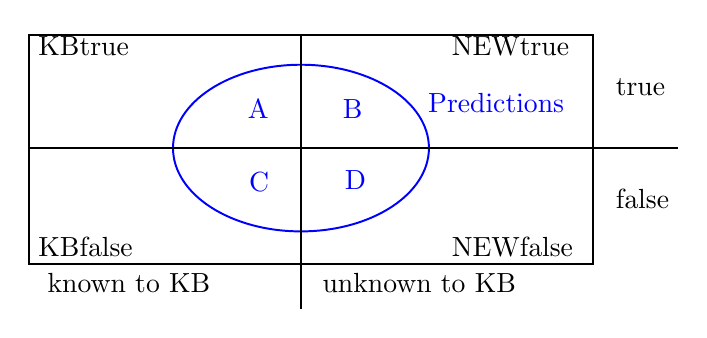
\begin{tikzpicture}

% Fabian: Keep figure in two colors.
% Even if printed in black and white, it's still clear enough

  \path[draw=blue, line width=0.7086614168764338] (3.708333, -1.458333) ellipse (1.625000 and 1.058333);
  \node[above, right, color=blue, font=] at (5.2000, -0.88333) {Predictions};
  \node[above, right, color=blue, font=] at (2.908333, -0.958333) {A};
  \node[above, right, color=blue, font=] at (4.116667, -0.966667) {B};
  \node[above, right, color=blue, font=] at (2.925000, -1.891667) {C};
  \node[above, right, color=blue, font=] at (4.141667, -1.866667) {D};
  \node[above, right, color=black, font=] at (0.250000, -0.166667) {KBtrue};
  \node[above, right, color=black, font=] at (0.250000, -2.708333) {KBfalse};
  \node[above, right, color=black, font=] at (5.500000, -0.166667) {NEWtrue};
  \node[above, right, color=black, font=] at (5.500000, -2.708333) {NEWfalse};
  \node[above, right, color=black, font=] at (7.583333, -0.683333) {true};
  \node[above, right, color=black, font=] at (7.583333, -2.100000) {false};
  \node[above, right, color=black, font=] at (0.366667, -3.166667) {known to KB};
  \node[above, right, color=black, font=] at (3.858333, -3.166667) {unknown to KB};
  \path[draw=black, line width=0.7086614168764338] (0.250000, -0.016667) rectangle (7.416667, -2.933333);
  \draw[draw=black, line width=0.7086614168764338] (0.250000, -1.458333) -- (8.500000, -1.458333);
  \draw[draw=black, line width=0.7086614168764338] (3.708333, -0.025000) -- (3.708333, -3.500000);
\end{tikzpicture}

\label{fig:prediction}
\end{figure}

Our goal is to find rules that make true predictions that go beyond the current KB.
In Figure~\ref{fig:prediction}, we wish to maximize the area B and to minimize the area D.
There are two obvious challenges in this context: First, the areas NEWtrue and NEWfalse are unknown.
So if we wish to maximize B at the expense of D, we are operating in an area outside our KB.
We would want to use the areas KBtrue and KBfalse to estimate the unknown area.
This, however, leads to the second challenge: Semantic KBs do not contain negative evidence.
Thus, the area KBfalse is empty.
This is the central challenge of our setting: to provide counterexamples for the rule mining.
These can take the role of KBfalse so that we can estimate the areas NEWtrue and NEWfalse.
We describe two approaches to this problem:
Creating counterexamples according to the Closed World Assumption (CWA) that traditional association rule mining systems apply and according to the Partial Completeness Assumption (PCA) that we propose.
We will now present these approaches in detail.
% There are several approaches to this problem:
% The standard confidence, the standard positive-only learning evaluation score of ILP, and the partial completeness assumption that we propose.
% We will now present these approaches in detail.



\subsection{The CWA and Standard Confidence} \label{subsubsec:stdConf}
The standard confidence measure takes all facts that are not in the KB (i.e., NEWtrue and NEWfalse) as negative evidence.
Thus, the standard confidence of a rule is the ratio of its predictions that are in the KB, i.e., the share of A (KBtrue) 
in the set of predictions:

\[conf(\vec{B} \Rightarrow r(x,y)) := \frac{supp(\vec{B} \Rightarrow r(x,y))}{\#(x,y): \exists z_1,...,z_m: \vec{B}}\]\\

\noindent Recall that the size of the set A is quantified by the support of the rule.
For instance, for Table~\ref{tab:exampleKB} and the rule $R:livesIn(x,y)\Rightarrow wasBornIn(x,y)$,
$conf(R)=1/3$, i.e., because (a) there is one positive example for the rule and (b) the predictions 
$wasBornIn(Adam, Rom)$ and $wasBorn(Bob,Zurich)$ are counted as negative examples as they do not appear in the KB.

Standard confidence is the measure traditionally used in association rule mining and market basket analysis, where the Closed World Assumption (CWA) is made:
if there is no evidence in any of the transactions of the database that a user bought a specific product, then this user did not buy the product.
Albeit natural for the market basket analysis scenario, standard confidence fails to distinguish between ``false'' and ``unknown'' facts,
which makes it inappropriate for a scenario with Open World semantics like ours. Moreover, we also pursue a different goal than market basket analysis:
we aim to maximize the number of true predictions that go beyond the current knowledge,
whereas market basket analysis usually tries to mine rules that can describe data that is already known.






\ignore{
\subsection{Positives-Only Learning}
For cases where the KB does not contain negative examples, Muggleton has developed a \emph{positives-only evaluation score} for ILP \cite{Muggleton:1996:LPD:647996.742465,usir1753}.
It takes random facts as negative evidence:
\[ Score := log(P)-log\frac{R+1}{Rsize+2}-\frac{L}{P} \]
Here, $P$ is the number of known true facts covered (KBtrue, or A resp., in Figure~\ref{fig:prediction}), $R$ is the number of random examples covered, $Rsize$ is the total number of randoms, and $L$ is the number of atoms in the hypotheses. \comment{Katja}{is ``randoms'' a well-defined term?}
The intuition is that a good rule should cover many positive examples, and few or no randomly generated examples. This ensures
that the rule is not overly general. Furthermore, the rule should use as few atoms as possible, and thus achieve a high compression.
This measure is implemented (among others) in the ALEPH system.

% \comment{Fabian}{Give intuitive reason why this measure is not good, to justify our own measure. Check:}
% The disadvantage of this measure is that it ``guesses'' negative examples at random.
% Even if a rule produces many false predictions, the intersection of these false predictions and the random counterexamples may be very small.
% In section~\ref{sec:experiments}, we compare ALEPH with our method.


%\comment{Fabian}{Give intuitive reason why this measure is not good, to justify our own measure.}
%\comment{Chris}{I gave it a try. Please have a look.} % Looks good, thanks!
% \comment{Fabian}{Thanks for the explications, Christina! Can we have a rule that is intuitively false? I tried to change the example, please modify if wrong.}

The disadvantage of this measure is that it ``guesses'' negative examples at random, whereas rules usually create false predictions in a non-random way.
Even if a rule produces many false predictions, the intersection of these false predictions and the random counterexamples may be very small.
Consider for example the rule $bornIn(x,y) \Rightarrow diedIn(x,y)$, which produces false predictions for example for persons who have moved
to a different place during their life.
By creating negative examples just by considering random person-location pairs,
we might not produce any case for which the rule will give a false prediction, % (person re-married with someone's mother),
simply because such a negative example will have a relatively small probability to be generated.
In section~\ref{sec:experiments}, we compare this measure to our method, which we introduce next.
}


\subsection{The PCA and the PCA-Confidence}\label{subsubsec:pcaConf}

In AMIE, we generate negative examples for a rule by means of the \emph{Partial Completeness Assumption} (PCA).
The PCA is the assumption that if $r(x,y) \in$ \emph{KBtrue} for some $x,y$, then
\[\forall y': r(x,y') \in \mbox{\emph{KBtrue}}\ \cup\ \mbox{\emph{NEWtrue}} \Rightarrow r(x,y') \in \mbox{\emph{KBtrue}}\]
In other words, we assume that if we know one $y$ for a given $x$ and $r$, then we know all $y$ for that $x$ and $r$.
This assumption allow us to generate counter-examples in a way that is less restrictive than the standard confidence.
In our example from Table~\ref{tab:exampleKB}, the PCA will assume that any other place of birth for 
Adam and Carl is false. Conversely, the PCA will not assume anything about the places of birth of Carl, because
the KB does not know any.
With this notion in mind, we redefine the definition of confidence for rules. Under the PCA, 
the denominator of the confidence formula is not the size of the entire set of conclusions 
derived from the body of the rule,
but the number of facts that we know to be true together with the facts that we assume to be false.

\begin{small}
\begin{equation} \label{eq:pcaConf}
 \hspace*{-2ex}
conf_{pca}(\vec{B} \Rightarrow r(x,y)) := \frac{supp(\vec{B} \Rightarrow r(x,y))}{\#(x,y): \exists z_1,...,z_m,y': \vec{B} \wedge r(x,y')}
\end{equation}
\end{small}

This formula normalizes the support by the number of pairs $(x,y)$ for which there exists a $y'$ with $r(x,y')$.
For the KB introduced in Table~\ref{tab:exampleKB} and the rule $R: livesIn(x,y)\Rightarrow wasBornIn(x,y)$,
$conf_{pca}(R)=1/2$, i.e., only $wasBornIn(Adam, Rom)$ counts as a negative example, 
because we already know a different place of birth for Adam. The prediction $wasBorn(Bob,Zurich)$ is completely disregarded as evidence.

Notice that Eq.~\ref{eq:pcaConf} fixes $x$ and $r$ and implies that rules will try to predict values for $y$. 
AMIE always predicts in the most functional direction. To see this, recall that 
it is more intuitive to predict the birthplace of a specific person 
than predict all the people that were born in a specific city.
Since in Sec.~\ref{subsec:functions} we re-write all relations so that their functionality 
is larger than their inverse functionality, the most functional direction 
will be always to predict $y$ given $x$.

In spite of being an assumption, the PCA is certainly true for functions, such as \emph{birthdate} and \emph{capital}.
The PCA also holds for relations that are not functions but that have a high functionality,
as we shall see in our qualitative analysis of the PCA in Section~\ref{pcaEvaluation}. 
The PCA has been applied in the Google Knowledge Vault under the name ``local completeness assumption'' \cite{knowledgevault}.






 %%%%%%%%%%%%%%%%%%%%%%%%%%%%%%%%%%%%%%%%%%%%%%%%%%%%%%%%%%%%%%%%%%%%%%%%%%%%%%%%%%%%%%%%%%%%%%%%%%%%

 % previous version from here


% \subsubsection{Qualitative Evaluation of the PCA}
% \label{pcaEvaluation}
%
% Since the PCA is one of the basic ingredients of AMIE,
% we wanted to know whether the PCA holds for a real world KB.
% For this purpose, we looked into each of the 33 relations between entities in YAGO2.
% For each relation $r$, we randomly sampled 30 subjects.
% For each subject $x$, we checked whether the KB knows all $y$ with $r(x,y)$.
% As a ground truth, we took the Wikipedia page of $x$ and what we could find on the Web by a search engine.
% It is obvious that such an evaluation cannot be done strictly quantitatively.
% For example, a person might have worked for a company, but this fact might appear nowhere on Wikipedia -- or even on the Web.
% Or a musician might play 10 instruments at different levels of proficiency, but Wikipedia mentions only the 4 main instruments.
% Even a search on the Web might not tell us that there are more than 4 instruments.
% Therefore, we resorted to a qualitative analysis.
% We analyzed each of the relations manually, and grouped the relations into categories.
% Some relations fall into multiple categories. \ignore{We also compare the PCA to the closed world assumption (CWA), i.e., the assumption that all facts that are not in the KB are false. This is the assumption on which the standard confidence measure relies.}
% % \comment{Fabian}{Could you check whether the relations you evaluated are placed right? (See spreadsheet) The relations with a question mark need additional checking...}
% %For this purpose, we randomly chose 30 entities and checked if there are missing facts about each entity-relation pair using the whole Web and common sense as ground truth.
% % Driven by these initial results that focused on answering the question whether the PCA holds for an average fact that is assumed to be false,
% % we also analyzed qualitatively whether the PCA holds for a particular entity-relation combination.
% % For this purpose, we randomly chose 30 entity-relation pairs and examined whether the assumption holds or not using the whole Web and common sense as ground truth.
% %\comment{Katja}{Is that true?}
% Table~\ref{PCA_assumption_entities} summarizes our findings.
% % by proposing a categorization of the problems we encountered and relating them to example relations that fall into these categories.
%
% % \ffigure{Table}{PCA_assumption_entities}{Categories of relations w.r.t. the PCA}{
% % \begin{tabular}{p{2cm}|p{5.4cm}}
% % \centering{Category}		  & Relations 	\\
% % \hline
% % Functions   & \emph{wasBornIn}, \emph{diedIn}, \emph{hasCapital}, \emph{hasCurrency*}, \emph{happenedIn}, \emph{hasPredecessor*}, \emph{owns}$^{-1}$ \\
% % Quasi-Functions & \emph{hasOfficialLanguage}, \emph{graduatedFrom}, \emph{isCitizenOf}, \emph{directed}$^{-1}$, \emph{hasAcademicAdvisor}, \emph{created}$^{-1}$, \emph{isLeaderOf}, \emph{wroteMusicFor?}$^{-1}$\\
% % \hline
% % Granularity Differences& 	$isLocatedIn$, \emph{happenedIn?}\\
% % \hline
% % Time Agnosticism \ignore{and implicit assumptions Fabian: What is this?} & $livesIn$, $worksAt$, $isCitizenOf?$, \emph{hasCapital?}, \emph{isMarriedTo}\\
% % % Implicit assumptions & $livesIn$, $isCitizenOf$\\
% % %Knowledge representation & $isMarriedTo$, $hasChild$, $actedIn$, $playsFor$, $worksAt$, $isPoliticianOf$\\
% % Extraction Incompleteness& \emph{participatedIn}$^{-1}$, \emph{produced}$^{-1}$,  \emph{actedIn}$^{-1}$, \emph{playsFor}, \emph{holdsPoliticalPosition}, \emph{hasChild}$^{-1}$, \emph{graduatedFrom}, \emph{hasWonPrize}, \emph{dealsWith}\\
% % %$influences$, $dealsWith$, $participatedIn$, $hasMusicalRole$, $livesIn$, $holdsPoliticalPosition$, $hasWonPrize$, $imports$, $exports$\\
% % Source Incompleteness & \emph{influences}$^{-1}$, \emph{imports}, \emph{livesIn}, \emph{holdsPoliticalPosition}, \emph{worksAt}, \emph{hasMusicalRole}, \emph{dealsWith}, \emph{isInterestedIn}, \emph{isKnownFor}
% % \end{tabular}
% % }
%
%
%
% \paragraph{Functions} YAGO2 contains several functions. For these, the PCA holds by definition.
% The PCA extends to relations that are not strictly speaking functions, but that have a high functionality.
% These are relations that usually have one object per subject, even though there could be multiple.
% For example, a person can graduate from several universities, but most people graduate from a single university.
% In all of these cases, the PCA worked very well, and predicted completeness correctly for $73\%-100\%$ of the subjects under investigation.
% Thanks to the FUN-property, the PCA also holds for quasi inverse-functional relations such as \emph{directed}.\\
%
%
% \ffigure{Table}{PCA_assumption_entities}{Categories of relations w.r.t. the PCA}{
% \begin{tabular}{p{2cm}|p{5.4cm}}
% \centering{Category}		  & Relations 	\\
% \hline
% Functions   & \emph{wasBornIn}, \emph{diedIn}, \emph{hasCapital}\\%,  \comment{Chris}{have we evaluated those guys?} \comment{Luis: }{These relations do not exist in YAGO2, only in YAGO2s} \emph{happenedIn}, \emph{hasPredecessor}, \emph{owns}$^{-1}$ \\
% \hline
% Quasi-Functions & \emph{hasCurrency}, \emph{hasOfficialLanguage}, \emph{graduatedFrom}, \emph{isCitizenOf}, \emph{directed}$^{-1}$, \emph{hasAcademicAdvisor}, \emph{created}$^{-1}$,  \emph{isLeaderOf}, \emph{isPoliticianOf}, \emph{isAffiliatedTo}\\%, \comment{Chris}{have we evaluated those guys?} \emph{wroteMusicFor}$^{-1}$\\
% \hline
% Granularity Differences& 	\emph{isLocatedIn},  \emph{livesIn}\\%,\comment{Chris}{have we evaluated those guys?} \emph{happenedIn}\\
% \hline
% Implicit Assumptions&\emph{livesIn} \\
% \hline
% Source Incompleteness & \emph{influences}$^{-1}$, \emph{imports}, \emph{exports}, \emph{actedIn}$^{-1}$, \emph{worksAt}, \emph{hasMusicalRole}, \emph{dealsWith}, \emph{isInterestedIn}$^{-1}$, \emph{isKnownFor}$^{-1}$\\
% \hline
% Extraction Incompleteness& \emph{participatedIn}$^{-1}$, \emph{isMarriedTo}, \emph{produced}$^{-1}$,  \emph{actedIn}$^{-1}$, \emph{playsFor}, \emph{holdsPoliticalPosition}, \emph{hasChild}$^{-1}$,  \emph{hasWonPrize}, \emph{dealsWith},\emph{influences}$^{-1}$, \emph{hasMusicalRole} \\
% \end{tabular}
% }
%
% \paragraph{Granularity Differences} Some relations, such as \emph{locatedIn} and \emph{livesIn}, hold between an entity and a geographical region.
% In that case, the region can be given at the granularity of a city, a region, a country, or a continent.
% Naturally, if YAGO contains one of these, the others are possible options, and thus the PCA does not hold.
% However, these cases could be addressed if one restricts the range of the relation.
% With such a restriction, the relations become functions or quasi-functions, which lifts them into the category where the PCA works well.
% We plan to investigate this possibility in future work.
%
% % \paragraph{Time Agnosticism} \comment{Chris}{I suggest to erase the time agnosticity.
% % What I meant back then is that the infobox might contain as residence only the last residence (and therefore YAGO knows only that one),
% %  but we take as correct all residences. I assume that we can consider this as a case of incomplete extraction.}
% % \comment{Fabian}{I think it makes an interesting special case, also with marriedTo}
% % For some relations, the KB is time agnostic: It contains only one object for a given subject, even though other objects may have held at other points of time.
% % For example, a person might have lived in many different places during her life and all the corresponding facts are considered to be true.
% % However, the KB might contain only the latest of these facts.
%
%
% \paragraph{Implicit Assumptions} Some statements can be inferred from the Wikipedia page even if the page does not mention them. % For instance, %\emph{livesIn} is incomplete ``in-purpose'' in the sense
% People do not usually state information that can easily be inferred by what they have stated before
% (following Grice's Maxim of quantity and manner~\cite{grice}). %\footnote{\url{http://www.usingenglish.com/articles/grices-conversational-maxims.html}}).
% For example, if someone graduated from a university, people usually do not feel obliged to mention that this person used to live in the country,
%  in which the university is located,
% because this can easily be inferred by the reader. Only less obvious residences will be explicitly mentioned and therefore, PCA assumption will not hold.
% Note that rules such as $graduatedFrom(x,y)\Rightarrow livesIn(x,y)$, to follow the previous example, can only be mined if Grice's maxims are occasionally violated by the authors of the articles.
% If the authors follow the maxims always, then such rules cannot be mined, because there are not even positive examples for which the rule holds (lack of support).
% In the case of YAGO, the only relation that we found in this category is \emph{livesIn}.
%
%
% \paragraph{Source Incompleteness} For many relations, the source itself (Wikipedia) is incomplete.
% Usually, these relations have, for each subject, some objects that are undisputed.
% For example, it is undisputed that Albert Einstein is interested in physics. However, these relations also have objects that are less important, disputed, or unknown.
% For example, Albert Einstein might also be interested in music (he played the violin), but maybe also in pancakes.
% These less prominent objects are a lot less likely to appear in Wikipedia, or indeed in any Web page.
% Even if they do, we can never be sure whether there is not still something else that Einstein was interested in.
% For these relations, the knowledge sources are often incomplete by nature.
% For example, not every single product that a country imports and exports is explicitly mentioned.
% Whether or not this poses a problem depends on the application.
% If ground truth is defined as what is universally true, then source incompleteness is a problem.
% If ground truth is the source of the KB (i.e., Wikipedia in this case), then source incompleteness is not an issue.
% \comment{Luis}{Does isMarriedTo fall in this category? What about non-prominent spouses (without Wikipedia article)? We would not extract the inverse statement in that case.}
% \comment{CHris}{This is the case of extraction incompleteness. Wikipedia usually is pretty precise for the spouses. So it is complete. The fact
% that yago does not extract spouses that do not have their own wikipedia pages is a problem with the extraction. Not an incompleteness
% problem}
%
%
% \paragraph{Extraction Incompleteness} For a large number of relations, the Wikipedia page contains more objects for a given subject than the KB.
% These are cases where the extraction process was incomplete.
% In the case of YAGO, this is due to a strong focus on accuracy,
% which causes the extraction to discard any extracted fact that cannot be type checked or linked to an entity.
% This class of relations is the most sensitive category for the PCA.
% The success of the PCA will depend on how many relations and to what extent they are affected by incomplete extractions.
% \comment{Chris}{Do we have precision numbers for this category?}
% % Furthermore, there are relations which are sometimes open to subjective interpretation.
% % For example, it is difficult to decide whether a particular person was actually influenced by another person that he or she met.
%
% \paragraph{Discussion} In summary, our analysis shows that it depends on the nature of the relation and on its type signature whether the PCA holds or not.
%  There are a large number of relations for which the PCA is reasonable.
% These are not just functions and inverse functions, but also relations that exhibit a similar behavior.
%
% For many other cases, the PCA does not hold. In these cases, AMIE will wrongly assume that a rule is making incorrect predictions -- although, in reality,
% the predictions might be correct.
% Thus, when the PCA does not hold, AMIE will err on the side of caution.
%
% At the same time, the PCA is not as restrictive as the closed world assumption (CWA):
% PCA admits that there can be facts that are true, but not known to the KB.
% \ignore{If we compare the PCA to the CWA, we note that the CWA assumes that all facts that are not in the KB are false. Consider a function $r$ and an entity $x$. If there exists an $y$ with $r(x,y)$ in the KB, then the CWA holds: Any fact of the form $r(x,y')$ with $y'\neq y$ is false. However, if there is no $y$ with $r(x,y)$, then the CWA does not hold. The CWA would wrongly assume that there cannot be a $y$ with $r(x,y)$. } For example, if a person has a birth date, then both CWA and PCA would not admit another birth date. However, if a person does not have a birth date, then the PCA will admit that there can be a birth date, while the CWA will assume that there cannot be a birth date. Thus, the PCA is more permissive than the CWA.
% This encourages us to use the PCA for the definition of our confidence. In our experiments, we will show that this definition of confidence produces
%  more predictive and more accurate rules than the standard confidence, which is based on the CWA.
%

 % previous version until here
 %%%%%%%%%%%%%%%%%%%%%%%%%%%%%%%%%%%%%%%%%%%%%%%%%%%%%%%%%%%%%%%%%%%%%%%%%%%%%%%%%%%%%%%%%%%%%%%%%%%%

%We will evaluate the PCA in the context of rule mining next.


% \comment{Fabian}{Old text follows. I tried to subsume it in the classification above. I would propose to remove what follows, for the reasons given below:}
%
%
% % PCA might be a reasonable assumption or not, depending on the nature of the head relation and its type signature.
% For example, for relations with strong functional or inverse functional behavior, such as $diedIn$ and $directed$,
% PCA successfully predicts negative facts (ratio=100\% in Table~\ref{PCA_assumption_rules}).
% On the other hand, $livesIn$ is a relation for which PCA does not hold.
% The reason for this is manifold; and results from both the type signature of $livesIn$ and its nature. For example, consider the rule $isCitizenOf(x,y) \rightarrow livesIn(x,y)$.
% If the KB contains the information in which city a specific person lives and the rule predicts the corresponding country, then the predicted fact is counted as negative although it is not because the city is located in the predicted country. This is also true for the relation $isLocatedIn$.
% In other words, PCA is sensitive to predictions that contain arguments involved in a strict functional hierarchical relation that expresses granularity, e.g., a particular city is in general located in a particular region, a region in a country, and so on.
% %A possible solution to counteract this problem is to consider the type system as well as the domain/range information that is provided by the KB. The approach proposed in this paper, however, still ignores such information but we plan to integrate this aspect in our future work.
% % In other words, PCA is sensitive to granularity effects that might exist between the different relations.
% % However, this issue might be tackled if in the future we make use of the type system and domain/range information of the KB, which for the time being we ignore.
%
% There is another problem category that the $livesIn$ relation falls into:
%
% \ignore{
% \comment{Chris}{Do we actually need the following one? I think it does not fit in this context. Perhaps move it to the model section?}
% \comment{Fabian}{I wrote it, but I think it should just be removed, unless someone protests}
% On the other hand, according to Grice's conversation maxims we should not say something that can lead to false conclusions.
% I.e., if someone states that Priscilla Presley has a child (which is not false but incomplete as she actually has two children),
% humans would infer that she has only one child and this is also how the PCA assumption would interpret the information.
% % On the other hand, if someone states that Priscilla Presley has one child, then this is not false but incomplete as she actually has two children.
% % However, humans would understand that she has not more than one child and this is also how the PCA assumption would interpret the information.
% %\comment{Fabian}{Interesting! Grice's maxim can also be used to explain why the PCA makes sense. Look at Priscilla. She has 2 children. If we say "Priscilla has 1 child", that is not false. But it is not complete. Thereby, we violate Grice's maxim.}
% This phenomenon makes information extraction very difficult and results in PCA being less accurate for some relations.
% }
% $worksAt$ and $isCitizenOf$ are additional examples of relations that are both time agnostic and often go along with implicit assumptions. \comment{Katja}{Split up into two categories?}
% In general, this group of relations is very difficult to capture because of the lack of information that can be exploited by machines
% and because it eventually requires to understand how the human brain works.
% But nevertheless, AMIE is able to mine such rules even though the predicted precision does not always exactly match the actual precision. \comment{Fabian}{Here, we do not yet talk of rules, do we?}
%
% We also noticed that for relations for which functionality and inverse functionality (Section~\ref{subsec:functions}) have similar values
% (e.g., $isMarriedTo$, $hasChild$), PCA might also show some deficiencies.
% For such relations it is not clear which variable is the input and which one is the output (e.g., parent or child, husband or wife).
% \comment{Fabian}{From the theoretical point of view, this is not a problem: If the KB contains people that have many children, then hasChild is de facto inverse functional, in China it is de facto functional.}
% In cases in which it is not clear if the fact relates more with the subject or the object we observe the following problem:
% the information about these relations is often scattered on Wikipedia pages of both entities in the relation,
% e.g., two persons might get married and only one of the Wikipedia pages is updated. \comment{Fabian}{We should not argue this way, because it basically means that we were too lazy to extract the information manually from Wikipedia. We could have manually scanned the download of Wikipedia (the XML dump) for the spouse, and we would have found him/her.}
% We have also found these problems to be true for several N:M relations such as $actedIn$ and $playsFor$.
% In summary, the problems that occur with these relations originate from the knowledge representation both in the KB
% as well as in the knowledge source, in our case Wikipedia.
% Since for these relations it is not clear which variable is input and which output, a possible solution that we plan to consider
% in our future work could be to mine two versions of a rule.
% For example when learning the relation $actedIn$, once actor is the input and movie the output and once the other way round.
%
% % Another source of problems are extraction failures, i.e., during the construction of the KB by extracting information from sources such as Wikipedia the content is misunderstood,
% %  which results in false facts in the KB. This is especially true for relations that are difficult to extract in general such as $dealsWith$ and $influences$.
% % \comment{Fabian}{Do we have really false extractions? Or only incomplete extractions? If we do, that would be an additional category}
% % As AMIE so far relies on the input contained in the KB and assumes facts in the KB to be true, this naturally leads to problems during rule mining.
%
% A possible solution would be to combine rule mining and knowledge extraction and use mutual feedback:
% the rule mining part can create "possibly true`` facts and then an information extraction component will try to extract exactly those facts from the source.
% If new facts can be added to the KB from the information extraction component, new rules can potentially be learned by the rule mining component.
% \comment{Fabian}{I love this idea! The problem is that the incompleteness kills the PCA, and thus AMIE will exactly not mine the ``expected'' rules and facts, no? It seems that we are shooting ourselves in the knee here...}

% \comment{Chris}{move to experiments or completely off}
%
% \subsection{PCA in Rule Mining}
% %\comment{Chris}{I moved it as a paragraph under the quality evaluation, because I think it logically belongs here. You can move it around if you wish.}
% We have seen that the PCA holds for some relations, but is too optimistic about the completeness of the KB for many others.
% We wanted to evaluate how this influences the rule mining in AMIE.
% Whenever AMIE mines a rule $\vec{B} \Rightarrow r(x,y)$, she will look at all facts that the rule can predict.
% Conceptually, AMIE will group the predictions into three categories:
% Either the prediction appears in the KB, then it is a positive example.
% The prediction can also be rejected by the PCA, and then it is a negative example.
% Finally, the prediction can be neither a positive example nor a negative example, but just an statement of unknown truth.
% Now, we are interested in the negative examples.
% These fall again into two categories: True negative examples ($TN$)  are statements that are false in reality ($TN \subseteq NEWfalse$).
% False negative examples ($FN$) are statements that were assumed to be false, but are true in reality ($FN \subseteq NEWtrue$).
% We want to measure how often the assumed negative examples were indeed negative examples.
% For this reason, we ran AMIE on YAGO\footnote{We used the version ``YAGO2''} and collected the resulting rules.
% For each rule, we sampled 30 predictions that the PCA called false negative examples.
% \comment{Fabian}{Did we do that for all rules? Or only for the rules with a high PCA confidence? If we did the latter, then we are not being fair, no?}.
% \comment{Chris}{It is only for the top 30 in PCA. }
% We manually evaluated them, using Wikipedia as ground truth.
% For each head predicate, we report the average of  $\frac{|TN|}{|TN+FN|}$ among all rules with this specific head,
% weighted by the total number of assumed negatives for each rule (micro-average).
% We call this measure $precOnNeg$:
%
% \[
%  precOnNeg(r_h)=\frac{\sum \limits_{all \; R \; with\; r_h \;in \; head }{ |TN(R)|}}{\sum \limits_{all \; R \; with\; r_h \;in \; head }{|TN(R)+FN(R)|} }
% \]
%
% The results are shown in Table~\ref{PCA_assumption_rules}.
% Our results show that the PCA works very well in practice:
% In the vast majority of cases where the PCA rejects a prediction, that prediction is indeed wrong.
% This is trivially true for functional relations such as \emph{diedIn}, but holds also for many other relations.
% \emph{livesIn} is a particularly hard case: It suffers from granularity differences and implicit assumptions.
% Hence, the PCA does not work well for this relation.
%
%  \ffigure{Table}{PCA_assumption_rules}{Ratio of facts correctly assumed to be false}{
% \begin{tabular}{l|c}
% %head predicate		  & $TN/(TN+FN)$ \% 	\\
% \textbf{Head Predicate} & $precOnNeg$ \% 	\\
% \hline
%   $created$		&86.67	\\
%   $diedIn$		&100	\\
%   $directed$		&100 	\\
%   $hasChild$		&60.74	\\
%   $hasOfficialLanguage$	&75	\\
%   $isCitizenOf$		&80.03	\\
%   $isLeaderOf$		&90	\\
%   $isMarriedTo$		&83.82	\\
%   $isPoliticianOf$	&73.15	\\
%   $livesIn$		&7.75	\\
%   $produced$		&93.87	\\
%   $worksAt$		&89.66	\\
% \end{tabular}
% }
% \comment{Fabian}{In the ideal case, we would compute the numbers for the CWA here and compare...}
%
% \paragraph{Discussion}
% %Note that despite these problems, % Fabian: There is no problem, PCA is great! :-)
% We see that the PCA performs well in general in the rule mining scenario.
% This is true in particular if we compare it to the alternative, the Closed World Assumption (CWA).
% The CWA would reject all statements that are not in the KB as false.
% This includes the statements that the PCA assumes to be false. Thus, there are cases in which both assumptions err.
% For example, if the KB contains only one parent of a child, then both assumptions would (erroneously) reject an additional parent.
% One way to mitigate this would be to learn an ``expected cardinality'' of a relation, and to reject as false everything that goes beyond this cardinality.
% This, however, would require coordination across rules if the number of objects in the KB falls more than 1 object short of the expected cardinality
% -- something that we defer to future work.
% \comment{Chris}{I didn't get it}
% In all other cases, the PCA is more accurate than the CWA:
% The CWA will not admit a birthplace for a person that does not have a birthplace in the KB. The PCA will.
% Likewise, the CWA will not admit parents for a child that does not have parents in the KB, while the PCA does.
% This shows that the PCA is more careful when producing negative examples. This will help AMIE mine more productive rules, as we shall see later.
% %Thus, even more facts are assumed to be false, i.e., all the facts that are not contained in the KB.
% %This set of facts consists of (i) facts assumed to be false under PCA and (ii) facts that normally exist for similar entities.
% %An error (FN) resulting from (i) could be that the KB contains, for example, only information about 1 out of 2 children ($childOf$). % Fabian: hasChild is inverse functional, the argument would have to be turned around.
% %For this case, both CWA and PCA would draw the wrong conclusion.
% %However, an error (FN) resulting from (ii) occurs if the KB, for example, does not contain a birthdate for a particular person;
% %under CWA, this means that the person has no birthdate whereas under PCA, this means that the fact is unknown.
%



%- - - - - - - - - - - - - - - - - - - - - - - - - - - - - -
\section{AMIE}
\label{sec:alg}
% !TEX root = main.tex

We now outline the core algorithm of AMIE and its implementation.
We follow the description in \cite{amie} and extend it with further explanations and details.

\subsection{Algorithm}
\label{subsec:algorithm}

%Only overview in this point
\paragraph{Algorithm} Algorithm~\ref{rm} shows our approach to mine rules. It takes as input a KB $\mathcal{K}$, a threshold $minHC$ on the head coverage of the mined rules, a threshold $minConf$ on the confidence, and a maximum rule length $maxLen$. We discuss the choice of parameter values further down.
The algorithm maintains a queue of rules (line~1), which initially contains all possible head atoms, that is, all rules of size 1.
It then iteratively dequeues a rule from this queue.
If the rule meets certain criteria (line~6), it is pushed to the output.
If the rule does not exceed the maximum number of atoms $maxLen$ (line~9), it goes through a refinement process (described below) which
expands the rule (the parent) to produce a set of new rules (the children). These new rules, 
if neither duplicates nor pruned by the head coverage threshold (line~12),  
are also pushed into the queue.
This process is repeated until the queue is empty. 
In the following, we will see in more detail the different phases of the algorithm.

\begin{algorithm}
\caption{Rule Mining}
\label{rm}
\begin{algorithmic}[1]
\Function{AMIE}{KB $\mathcal{K}$, $minHC$, $minConf$, $maxLen$}
    \State $q = [r_1(x,y), r_2(x,y) \dots r_m(x,y)] $
    \State $out = \langle \rangle$
	\While{$\neg q$\emph{.isEmpty}()}
	  \State $r = q.$\emph{dequeue}()
	  \If{$AcceptedForOutput(r, out, minConf)$}
	      \State $out.$\emph{add}$(r)$	
	  \EndIf
	  
	  \If{$length(r) < maxLen$}
	    \State $R(r) = Refine(r)$	    
	    \ForAll{rules $r_c \in R(r)$}  
		    \If{$hc(r_c) \ge minHC$ \& $r_c \notin q$}
			\State $q.$\emph{enqueue}$(r_c)$		      
		    \EndIf
	    \EndFor
	    
	  \EndIf  
	  
	\EndWhile
    \State \Return $out$
\EndFunction
\end{algorithmic}
\end{algorithm}

\paragraph{Refinement}\label{subsubsec:refinement}
One of the major challenges of rule mining is to find an efficient way to explore the search space. 
The naive algorithm of enumerating all possible combinations of conjunctions of atoms is infeasible for large KBs.
Hence, we explore the search space by iteratively extending rules using a set of \emph{mining operators} (line~10 of Alg.~\ref{rm}).
We see a rule as a sequence of atoms. The first atom is the head atom and the others are the body atoms. 
In the process of traversing the search space, we can extend a rule by using one of the following operators:
\begin{enumerate}
\item \textbf{Add Dangling Atom ($\mathcal{O}_D$})\\
This operator adds a new atom to a rule. The new atom uses a fresh variable for one of its two arguments. The other argument is a variable
that is shared with the rule, i.e., it occurs in some other atom of the rule.
\item \textbf{Add Instantiated Atom ($\mathcal{O}_I$})\\
This operator adds a new atom to a rule that uses an entity for one argument and shares the other argument (variable or entity) with the rule.
\item \textbf{Add Closing Atom ($\mathcal{O}_C$})\\
This operator adds a new atom to a rule so that both of its arguments are shared with the rule.
\end{enumerate}
Note that all above operators create connected rules.
By repeated application of these operators, we can generate the entire space of rules as defined in Section~\ref{sec:preliminaries}.
The operators generate even more rules than those that we are interested in, because they also produce rules that are not closed.
An alternative set of operators could consist of $\mathcal{O}_D$ and an operator for instantiation.
But these operators would not be monotonic, in the sense that an atom generated by one operator can be modified in the next step by the other operator.
Therefore, we chose the above 3 operators as a canonic set. We will describe in Section \ref{subsec:countqueries} how these operators are executed on the KB.

\begin{algorithm}
\caption{Decide whether to output a rule}
\label{pfo}
\begin{algorithmic}[1]
\Function{AcceptedForOutput}{rule $r$, $out$, $minConf$}
    \If{$r$ is not closed $\vee\; conf_{pca}(r) < minConf$}
      \State \Return $false$
    \EndIf 
    \State $parents = parentsOfRule(r, out)$
    \ForAll{$r_p \in parents$}
      \If{$conf_{pca}(r) \le conf_{pca}(r_p)$}
	\State \Return $false$
      \EndIf
    \EndFor
    \State \Return $true$
\EndFunction
\end{algorithmic}
\end{algorithm}

\paragraph{When to Output}\label{subsubsec:whenToOutput}
Not every rule that the mining algorithm dequeues is output. This is because some rules may not be closed, or may not be better than rules that have already been output. Algorithm~\ref{pfo} explains how we decide if a rule should be output or not once it has been dequeued.
The algorithm first checks if the rule is of the form described in Section~\ref{sec:preliminaries} (i.e., closed and connected).
The refinement operators used by AMIE (see Section~\ref{subsubsec:refinement}) always produce connected rules. 
So, at this point, the algorithm only checks if the rule is closed. Then, the algorithm calculates
the confidence of the rule and performs a quality check. The rule should have a confidence value that (i) passes the confidence threshold (line~1)
and (ii) improves over the confidence of all its parents (line~7).
The latter condition implies that the refinements of a rule ($B_1 \wedge ... \wedge B_n \wedge B_{n+1} \Rightarrow H$) must 
bring some confidence gain with respect to the parent rule
($B_1 \wedge ... \wedge B_n \Rightarrow H$). Since support and head coverage are monotonic metrics, 
we know that the child rule will never have a higher score than its parent rule. 
If the child rule has also lower confidence, then its quality is worse in all aspects than the parent rule. Hence, there is no reason to output it.

A rule can have several parents. For example, the rule $actedIn(x,y) \wedge directed(x,y) \Rightarrow created(x,y)$
can be derived by either adding $directed(x,y)$ to  $actedIn(x,y) \Rightarrow created(x,y)$ or by adding $actedIn(x,y)$ to
$directed(x,y) \Rightarrow created(x,y)$. AMIE requires a confidence gain over all parents of a rule.

Note that the decisions made at this point affect only the output. They do not influence the refinement process. i.e., a rule with low confidence can still be refined to obtain new rules.
This is because confidence is a non-monotonic measure, i.e. we might get good rules with further refinement of bad rules.


\comment{Fabian}{We have to justify the parameters at some point. Since we don't do it in the experiments, we should do it here... Please check.}
\comment{Luis}{The section Pruning became obsolete so I am merging it with the section parameters.}
\paragraph{Parameters and Pruning} 
If executed naively, Algorithm~\ref{rm} will have prohibitively high runtimes.
The instantiation operator $\mathcal{O}_I$, in particular, generates atoms in the order of $|\mathcal{R}| \times |\mathcal{E}|$.
For this reason the algorithm defines some parameters that determine when to stop with the exploration of the space. 
These are the minimal head coverage $minHC$, the minimal confidence $minConf$ and the maximal length $maxLen$.
% The algorithm traverses the search space and enumerate all rules that fulfil the constraints 
% of a minimal head coverage $minHC$, a minimal confidence $minConf$, and a maximal length of $maxLen$. 
%Thus, these parameters define when the algorithm shall stop with the exploration of the space. 
Choosing larger thresholds on head coverage, and choosing a shorter maximum rule length will make the algorithm stop earlier 
and output fewer rules. Relaxing the values will make the algorithm output the very same rules as before, 
and find also rules with a smaller head coverage or a larger number of atoms. 
Thus, these parameters define a trade-off between the runtime and the number of rules. 
Interestingly, a larger number of rules is not necessarily a good thing. 
For instance, a rule that covers only 1\% or less of the instances of a relation is probably not interesting 
(lack of statistical significance). Therefore, we set the default value $minHC=0.01$. Additionally, 
we show in our experiments that rules with more 
than 3 atoms tend to be very convoluted and not insightful. Hence, we set $maxLen=3$.

The same rationale can be applied to the confidence of a rule. A rule with confidence 10\% will make correct predictions one out of
ten times. Assuming that a user is not interested in such kind of rules, we set the default value $minConf=0.1$. 
Notice also that Algorithm~\ref{rm} does not use confidence for pruning. This implies that the confidence
threshold does not have a significant impact in the runtime as head coverage and maximum length.
% Likewise, a rule that covers only 1\% or less of the instances of a relation is probably not interesting. 
% Therefore, we set the default value $minHC=0.01$. We show in our experiments that rules with more 
% than 3 atoms tend to be very convoluted and not insightful. 
% Hence, we set $maxLen=3$. 

That being said, if the user is interested in less confident, more complex, or less supported rules, 
she can change these thresholds. However, we believe that there is no good reason to deviate from the default values. 
In particular, relaxing these values will not output better rules. This makes AMIE a system that can be run off the shelf, 
without the need for parameter tuning.

\ignore {
\paragraph{Pruning}
If executed naively, Algorithm~\ref{rm} will have prohibitively high runtimes.
The instantiation operator $\mathcal{O}_I$, in particular, generates atoms in the order of $|\mathcal{R}| \times |\mathcal{E}|$.
We first observe that we are usually not interested in rules that cover only very few facts of the head relation.
Rules that cover, for example, less than 1\% of the facts of the head relation can safely be assumed to be marginal.
Therefore, we choose $minHC=0.01$ as a lower bound for the head coverage. We observe that head coverage decreases monotonically as we add more atoms.
This allows for safely discarding any rule that trespasses the threshold (line~12 of Alg.~\ref{rm}).
Recall from Section~\ref{subsec:statSignificance} that support and head coverage are defined even for rules that are not yet closed, allowing for early pruning.
}
\paragraph{Duplicate Elimination} \label{subsec:duplicateElimination}
As mentioned in Section~\ref{subsubsec:whenToOutput} a rule can be derived in multiple ways.
For example, the rule $actedIn(x,y) \wedge directed(x,y) \Rightarrow created(x,y)$ can result from the application
of the operator $\mathcal{O}_C$ to both $actedIn(x,y) \Rightarrow created(x,y)$ and $directed(x,y) \Rightarrow created(x,y)$.
For this reason, AMIE checks for the existence of duplicate rules (line~12) in order to avoid queueing the same rule multiple times.
While checking two rules for equality is expensive (it is a graph isomorphism verification task), 
we observe that two rules can only be equal if they have the same head relation, the same number of atoms and
the same head coverage (or support). This reduces drastically the set of rules that have to be checked and therefore
the time invested in this task.


\paragraph{Multithreading}
To speed up the process, our implementation parallelizes Algorithm~\ref{rm}, that is, the main loop (lines~4 to~17) runs in multiple threads. 
This achieved by synchronizing the access to the centralized queue from which the threads dequeue and enqueue and the access to the output.
%In addition, when AMIE uses multiple threads, there is a need for an additional duplicate-elimination check at line~6 of Alg.~\ref{rm}. \comment{Fabian}{Can we avoid the discussion of dup elimination in the output here? I am afraid it might raise more questions than it anwers...}

\ignore{
\comment{Chris}{@Luis: why don't you use barriers here? I.e. all threads wait until there is no rule length n in the queue before moving to the rules with length n+1. For rules with 3 atoms in the body 
you will only have 2 synchronization points.}
Recall that our algorithm performs a breadth-first-search. 
This means that in a fully sequential execution, all the rules of size $n-1$ are always queued before all the rules of size $n$. 
It follows that, by the time we check the duplicates of a rule of size $n$ to enqueue it (line~12 in Algorithm~\ref{rm}), 
no rule of size $n$ has still been dequeued. In other words, if a rule is the duplicate 
of another rule already derived, the original rule must be in the queue. This property guarantees no duplicates at output time. 

However, this does not hold in a multi-threading environment. 
To see this, imagine that rules 
$R_n$ and $R'_n$ are both in the queue at timestamp $t_0$ and both can refined into rule $R_{n+1}$
by means of the mining operator $o$. 
Moreover, consider two threads $T_1$ and $T_2$ and the sequence of events depicted in Table~\ref{tab:duplicates}.

\begin{table}
\centering
 \begin{tabular}{c|l|l}
  Timestamp & $T_1$ & $T_2$\\  \hline
  $t_1$ & $R_n = q.dequeue()$	&  \\
  $t_2$ & & $R'_n = q.dequeue()$ \\
  $t_3$ & $R_{n+1} = o(R_n)$  & \\
  $t_4$ & $q.enqueue(R_{n+1})$  & \\
  $t_5$ & $R_{n+1} = q.dequeue()$ & \\
  $t_6$ & & $R_{n+1} = o(R'_n)$ \\
  $t_7$ & & $q.enqueue(R_{n+1})$ \\
\end{tabular}
\caption{An execution scenario that could lead to duplicate rules in the output.}\label{tab:duplicates}
\end{table}

In this example, we enqueue the rule $R_{n+1}$ twice, at timestamps $t_4$ and $t_7$. 
Since $T_1$ dequeues $R_{n+1}$ before $T_2$ also finds it, 
we cannot know that the rule was already output before. 
Since duplicate verification
can be performed very efficiently, we show that the time invested in this additional step does not  
outweight the benefit of using multiple threads.
}


\subsection{Count Projection Queries}
\label{subsec:countqueries}

AMIE tries to expand a given rule by applying all mining operators defined in the last section (one each time). 
We now explain how the operators are implemented and executed on a KB.

\paragraph{Count Projection Queries} 
%Each operator expects as input a variable that the new atom shall share with the existing rule. 
Assume that AMIE needs to add the atom $r(x,y)$ to a rule. 
For efficiency reasons, we do not blindly try all possible relations in the place of $r$. Instead, we first 
find all relations that lead to a new rule that passes the head-coverage threshold.
In other words, we first fire a \emph{count projection query} of the form

\indented{
SELECT $\bm{r}$, COUNT($H$)\\
WHERE $H \wedge B_1 \wedge ... \wedge B_{n-1}\; \wedge\; \bm{r}(\bm{X},\bm{Y})$\\
SUCH THAT COUNT($H$)$\geq k$
}

\noindent where $k := minHC \times size(H)$ (see Section~\ref{par:headCoverage}) is the translation of the
head coverage threshold into an absolute support threshold and the expression COUNT($\cdot$) has for the rest of this section COUNT(DISTINCT $\cdot$) semantics.
$\bm{X}$ and $\bm{Y}$ can represent variables that are either fresh or already present in the rule.
\comment{Luis}{About the meta-variables, the text originally said 
``that can be either variables or constants, depending on the type of atoms that the operator generates". I changed
because in principle we never add atoms where one of the arguments is a constant, because we first find the relation
and then the constants for the arguments.}
The results for $\bm{r}$ are the relations that, once bound in the query, ensure that the head coverage of the rule $B_1 \; \wedge ... \wedge B_{n-1} \;\wedge\; \bm{r}(\bm{X},\bm{Y}) \Rightarrow H$ is greater than $minHC$.
Notice also that for each value of $\bm{r}$, the expression COUNT($H$) gives us the support of the new rule.
We now discuss the cases for all three operators.

\paragraph{Dangling Atom Operator} 
% When we apply the $\mathcal{O}_I$ operator, at least one of this meta-variables binds to a constant.
As an example, assume that Algorithm~\ref{rm} dequeues the following intermediate non-closed rule for further specialization:

\indented{
\emph{marriedTo}$(x,z) \Rightarrow $ \emph{livesIn}$(x,y)$
}

\noindent
The application of the operator $\mathcal{O_D}$ will fire queries of the form:

\indented{
SELECT $\bm{r}$, COUNT($livesIn(x,y)$) WHERE  \\
$livesIn(x,y) \; \wedge \; marriedTo(x,z) \wedge \bm{r}(\bm{X}, \bm{Y})$\\
SUCH THAT COUNT($livesIn(x,y)$)$\ge k$
}

\noindent with 
\indented{
$\bm{r}(\bm{X}, \bm{Y}) \in \{\bm{r}(x,w), \bm{r}(z,w), \bm{r}(w,x), \bm{r}(w,z) \}$
}

\noindent That is, $\bm{r}(\bm{X}, \bm{Y})$ binds to each possible join combination of a new dangling atom,
where $w$ is an arbitrary fresh variable. For intermediate rules, dangling atoms are joined on the non-closed variables; 
$z$ and $y$ in this example.
If the rule is closed, dangling atoms are joined on all the variables appearing in the rule.

\paragraph{Closed Atom Operator} The $\mathcal{O_C}$ operator works in the same fashion. In our example, the atom $\bm{r}(\bm{X}, \bm{Y})$ 
can take values in $\{ \bm{r}(z,y), \bm{r}(y,z) \}$. The method will produce new atoms so that all open variables are closed. In this example, the method produces the minimum number
of specializations required to close the variables $y$ and $z$. If there is only one closed variable, the method will produce atoms between
the open variable and all the other variables. If the rule is already closed, the operator tries with
all possible pairs of variables in the rule.

\paragraph{Instantiated Atom Operator} The operator $\mathcal{O_I}$ is implemented in two steps. 
We first apply the operator $\mathcal{O_D}$ to produce a set of intermediate rules 
with a new dangling atom and a new fresh variable.
Then for each rule, we fire a count-projection query on the fresh variable. 
This step provides bindings for one of the arguments of the relation.
For instance, the implementation of the $\mathcal{O_I}$ operator to our example 
rule 

\indented{
\emph{marriedTo}$(x,z) \Rightarrow $ \emph{livesIn}$(x,y)$
}

\noindent will first add all possible dangling atoms to the rule. Let us consider one group of such atoms, e.g., those of the form
$\bm{r}(x,w)$. Then for each
value of $\bm{r}$ that keeps the rule above the head coverage threshold $minHC$, the algorithm tries to find the best bindings for 
$w$. For example, imagine we bind $\bm{r}$ to the relation $citizenOf$. The second step will fire a query of the form:

\indented{
SELECT $\bm{w}$, COUNT($livesIn(x,y)$) WHERE \\ 
$livesIn(x,y) \wedge marriedTo(x,z) \wedge citizenOf(x,\bm{w})$ \\
SUCH THAT COUNT($livesIn(x,y)$)$\ge k$
}

\noindent Each binding of $\bm{w}$ forms a new rule that will be enqueued and later evaluated for output.

Count-projection queries allow us to choose the relationships and entities for the operators 
in such a way that the head coverage for the new rules is above $minHC$.
We discuss how to implement count projection queries efficiently in Section~\ref{subsec:implementation}.

\subsection{Query Implementation Details}
\label{subsec:implementation}

\paragraph{In-memory Database} We have shown \cite{amie} that count projection queries translate into very inefficient queries in both SPARQL and SQL. Therefore, we have implemented an in-memory database that is specifically geared towards this type of queries.
Our implementation indexes the facts aggressively with one index for each permutation of 
the columns subject (\texttt{S}), relation (\texttt{R}), and object (\texttt{O}), i.e., there are six indexes, namely \texttt{SRO}, \texttt{SOR}, \texttt{RSO}, \texttt{ROS}, \texttt{OSR} and \texttt{ORS}. We call them \emph{fact indexes}.
Each fact index is a hash table, which maps elements of the first column to a nested hash table. This nested hash table maps elements of the second column to a set of elements of the third column. For example, the index \texttt{ORS} has as keys the objects of all triples in the KB. It maps each object $o$ to a hash table. This hash table has as keys all possible relations of the KB. It maps each relation $r$ to a set of subjects $\{s_1,...,s_n\}$, such that $r(s_i, o)$ for $i=1...n$.
Fact indexes allow us to check the existence of a triple in constant time. They also allow us to efficiently fetch the instantiations of an atom.

%where the keys are the values for the first column and the items are again hash tables. The nested hash tables map values of the second column to sets of values of the third column. 
%Figure~\ref{indexes} illustrates the structure of the fact index \texttt{RSO} for a set of four facts.
% 
% \begin{figure}
% %\hspace*{-5ex}
% 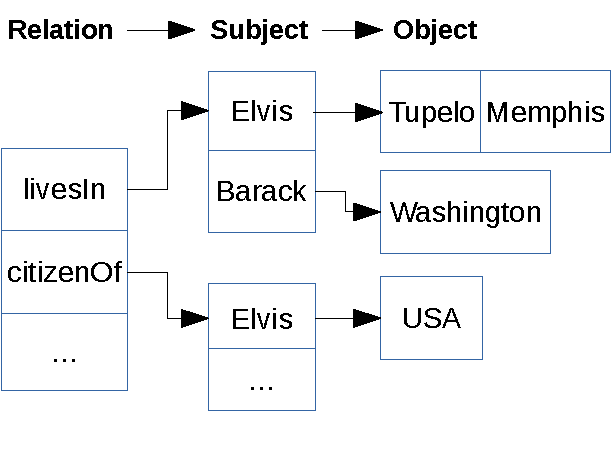
\includegraphics[width=0.5\textwidth]{figures/indexes}\
% \caption{Structure of the fact index RSO for a set of four facts}
% \label{indexes}
% \end{figure}

In addition to the fact indexes, our database relies on three \emph{aggregated indexes} \texttt{S}, \texttt{P}, \texttt{O}. These store the aggregated number of facts for each
key of the fact indexes. For example, the aggregated index \texttt{P} stores the number of triples for each relation in the KB, whereas the aggregated index \texttt{S} stores the number of triples where each entity appears as subject. 

\paragraph{Size Queries} Fact indexes in combination with aggregated indexes can be used to determine the \emph{size of an atom} ($size(a)$), i.e., its number of bindings in the KB. For example, the size of the atom $livesIn(x,y)$ can be retrieved by a simple look-up 
in the aggregated index \texttt{P}. The size of the atom $livesIn(x, USA)$ requires two 
lookups in the fact index \texttt{ROS}: the first lookup to get the object values of $livesIn$ and the second
to retrieve the list of subjects for the object value $USA$.
%If an atom has size greater than zero, it means that there exists a query answer for it in the KB.
% Fabian: let's not mix existence and sizes here (even though it's trivial, I agree)...

\paragraph{Existence Queries} One of the central tasks of the in-memory database is to determine whether there exists a binding for a conjunctive query. Algorithm~\ref{exists} shows how this can be implemented.  The algorithm requires as input a conjunctive query and a KB $\mathcal{K}$.
If the query is a single atom (Line 3), we can directly verify if its size is greater than zero using
the indexes (Line 4). Otherwise, we select the atom $B_s$ with fewest instantiations using the indexes (Line 6), 
and run through all of its instantiations (Lines 8 to 13). We apply such instantiations to the remaining atoms (Line 9)
and repeate this process recursively (Line 10) until we end up with a single atom. Since rules are connected query patterns, the atom $B_s$ must share at least
one variable with the remaining atoms. This means that by instantiating $B_s$, some variables in the remaining atoms 
become instantiated, making the atoms more selective with every recursive step.

\begin{algorithm}
\caption{Existence Queries}
\label{exists}
\begin{algorithmic}[1]
\Function{Exists}{$B_1 \wedge ... \wedge B_n$, $\mathcal{K}$}
    \State $q := B_1 \wedge ... \wedge B_n$
    \If {$n = 1$}
      \State \Return size($B_1$, $\mathcal{K}$) $> 0$
    \Else
      \State $s := argmin_i\;\{ size(B_i, \mathcal{K}) \}$
      \State $q := q \setminus \{ B_s \} $
      \ForAll {instantiations $b_s \in B_s$}
	\State Replace $b_s$ in $q$
	  \If{Exists($q$, $\mathcal{K}$)}
	    \State \Return true
	  \EndIf
      \EndFor
    \EndIf
    \State \Return false
\EndFunction
\end{algorithmic}
\end{algorithm}

\paragraph{Select Queries} 
Algorithm~\ref{select} describes the implementation of SELECT DISTINCT queries on one projection variable for a conjunction of
atoms. 
The algorithm starts finding the atom with the fewest number 
of instantiations $B_s$. If the projection variable $x$ is in $B_s$ (Lines 5 to 11), 
the algorithm goes through all the instantiations $\hat{x}$ of $x$, instantiates
the query accordingly and checks whether there exists a solution for the instantiated query pattern in the KB (Line 8). 
If there is, the solution $\hat{x}$ is added to the result set. In contrast, if the projection variable is not in the most 
restrictive atom $B_s$ (Lines 13 to 17), the algorithm iterates through the instantiations of $B_s$ and recursively selects the distinct
bindings of $x$ in the remaining atoms (Line 16).

\begin{algorithm}
\caption{Select Distinct Queries}
\label{select}
\begin{algorithmic}[1]
\Function{Select}{$\bm{x}$, $B_1 \wedge ... \wedge B_n$, $\mathcal{K}$}
    \State $q := B_1 \wedge ... \wedge B_n$
    \State $s := argmin_i\;\{ size(B_i, \mathcal{K}) \}$
    \State $result := \lbrace \rbrace$
    \If{$\bm{x} \in B_s$}
      \ForAll {instantiations $\hat{x} \in \bm{x}$}
	\State Replace $\hat{x}$ in $q$
	\If {Exists($q$, $\mathcal{K}$)}
	  \State $result$.add($\hat{x}$)
	\EndIf
      \EndFor
    \Else
      \State $q := q \setminus \{ B_s\}$
      \ForAll{instantiations $b_s \in B_s$}
      	\State Replace $b_s$ in $q$
      	\State $result$.add(Select($\bm{x}$, $q$, $\mathcal{K}$))
      \EndFor
    \EndIf
    \State \Return $result$
\EndFunction
\end{algorithmic}
\end{algorithm}

\paragraph{Count Queries} To compute the confidence of a rule $\vec{B} \Rightarrow r(x, y)$, AMIE must fire a \emph{count query} to estimate the denominator
of the confidence formula. For the PCA confidence, such queries have the form:

\indented{
SELECT COUNT($x$, $y$) WHERE $r(x, y') \wedge \vec{B}$
}

\noindent where $x$, $y$ are the variables in the head atom of the rule, $\vec{B} = B_1, \dots, B_n$ are the body atoms and $r(x,y')$ 
is a variant of the head atom where the least-functional variable has been replaced by a fresh variable $y'$ (see Section~\ref{subsubsec:pcaConf}).
These queries return the number of distinct bindings of the head variables 
that fulfil the pattern $r(x, y')\; \wedge\; \vec{B}$ and are used to
calculate the confidence of rules. The in-memory database first fires a SELECT query on variable $x$: 

\indented{
SELECT DISTINCT $x$ WHERE $r(x, y') \wedge \vec{B}$
}

\noindent Then, for each binding of $x$, it instantiates the query and fires another select query on variable $y$, adding up the number of instantiations.


\paragraph{Count Projection Queries} Count projection queries
take the form
\indented{
SELECT $\bm{x}$, COUNT($H$) WHERE $H \wedge B_1 \wedge ... \wedge B_n$\\
SUCH THAT COUNT($H$)$\geq k$
}
These are the types of queries used to determine the relations and instances for new atoms in the refinement
phase of AMIE. Algorithm \ref{algi} shows how we answer these queries. The algorithm takes as input a selection variable $\bm{x}$, a projection atom $H:=R(\bm{X},\bm{Y})$, remaining atoms $B_1, ... B_n$, the threshold $k$, 
and a KB $\mathcal{K}$. 
The algorithm returns a hash table with each instantiation of the selection variable 
$\bm{x}$ as key and the number of distinct bindings of the projection atom $H$ as value. 
\comment{Fabian}{I added the threshold k to this algorithm, to disentangle the roles of the rule mining and the in-memory database}
%The algorithm does not consider the threshold condition (SUCH THAT), because this condition is actually enforced by the AMIE algorithm and not the in-memory database. 

We first check whether $\bm{x}$ appears in the projection atom (Line 3).
If that is the case (Lines 4 to 10), we run through all instantiations of the projection atom, instantiate the query accordingly (Line 6), and check for existence (Line 7).
Each existing instantiation increases the counter for the respective value of the selection variable $\bm{x}$ (Line 8). 
If the selection variable does not appear in the projection atom (Lines 12 to 18), 
we iterate through all instantiations of the projection atom.
We instantiate the query accordingly, and fire a SELECT DISTINCT query for $\bm{x}$ (Line 14). 
We then increase the counter for each value of $\bm{x}$ (Line 16).

\begin{algorithm}
\caption{Count Projection Queries}
\label{algi}
\begin{algorithmic}[1]
\Function{SELECT}{$\bm{x}$, $R(X,Y) \wedge B_1 \wedge ... \wedge B_n$, $k$, $\mathcal{K}$}
    \State $map = \{\}$
    \State $q=B_1 \wedge ... \wedge B_n$
    \If {$\bm{x} \in \{R,X,Y\}$}
	  \ForAll{instantiations $r(x,y) \in R(\bm{X}, \bm{Y})$}
	    \State In $q$, replace $R$ by $r$, $X$ by $x$, $Y$ by $y$
	    \If{Exists($q$, $\mathcal{K}$)}
		\State $map[x]++$
	    \EndIf
	  \EndFor
	\Else
	  \ForAll{instantiations $r(x,y) \in R(\bm{X},\bm{Y})$}
	    \State In $q$, replace $R$ by $r$, $X$ by $x$, $Y$ by $y$
	    \State $\mathcal{X} :=$ Select($\bm{x}$, $q$, $\mathcal{K}$)
	    \ForAll{$x \in \mathcal{X}$}
		  \State $map[x]++$
	    \EndFor
	  \EndFor
	\EndIf
	\State $map := \{ \langle x \rightarrow n\rangle \in map : n \geq k\}$
	\State \Return $map$
\EndFunction
\end{algorithmic}
\end{algorithm}

\ignore{Fabian: This part no longer makes sense when we removed the SQL queries

\paragraph{Summary}
The AMIE algorithm iteratively builds more complex rules from simpler rules by the help of three operators.
It takes advantage of monotonic measures to prune the search space efficiently and also takes care of duplicate elimination.
We have identified projection queries as the crucial type of queries for rule mining.
Since standard database systems and standard SPARQL systems provide no specifically tuned support for these queries,
we have implemented a vanilla in-memory database, which has specific support for projection queries.
Our entire implementation is in Java. The code can be downloaded from our Web site\footnote{\url{http://mpi-inf.mpg.de/departments/ontologies/projects/amie}}.
}

%%% Uncomment this to return to the version with SQL queries.
% 
% \ignore{
% 
% %%%%%%%%%%%%%%%%%%%%%%%%%% Luis version under this point
% 
% \www{
% %After having outlined the preliminaries and the mining model in Sections~\ref{sec:preliminaries} and \ref{sec:pca},
% We now outline the core algorithm of AMIE and its implementation.
% %Again, we follow the explications in \cite{amie}.
% We follow the explications in \cite{amie} and extend them with further explanations and details.
% }
% 
% \www{
% %- - - - - - - - - - - - - - - - - - - - - - - - - - - - - -
% \subsection{Algorithm}
% \label{subsec:algorithm}
% \comment{R2}{Similarly, the Algorithm 2 is not very accurate. It would be clearer if "distinct" is added on line 15: "for all distinct x $\in$ SELECT ?x FROM K WHERE q do." (In contrast, the DISTINCT in the query on the top of Page 11 is redundant).}
% 
% \comment{R3}{Here are some of my criticisms, which apply to Section 5 on AMIE - your previous work:
% 1.Algorithm 1 is too high level and as such it leaves too much unexpressed (e.g. "execute in parallel", "is not pruned for output").
% 2.      SQL and SPARQL are presented at page 11 only to say that they are discarded for a custom implementation.
% 3.      The "vanilla in-memory database" implementation is too informally described (e.g.: each "index is a map from the first item to a map from the second item to a set of the third item": a more formal description and a figure, please!
% }
% 
% \paragraph{Goal} Our goal is to mine rules of the form defined in Section~\ref{sec:preliminaries}.
% One of the main problems of any mining approach is to find an efficient way to explore the search space. The naive algorithm of enumerating all possible rules is infeasible for large KBs.
% Hence, we explore the search space by iteratively extending rules by \emph{mining operators}.
% }
% 
% \www{
% \paragraph{Mining Operators}
% We see a rule as a sequence of atoms. The first atom is the head atom and the others are the body atoms. In the process of traversing the search space, we can extend a rule by using one of the following operators:
% \begin{enumerate}
% \item \textbf{Add Dangling Atom ($\mathcal{O}_D$})\\
% This operator adds a new atom to a rule. The new atom uses a fresh variable for one of its two arguments. The other argument is a variable
% that is shared with the rule, i.e., it occurs in some other atom of the rule.
% \item \textbf{Add Instantiated Atom ($\mathcal{O}_I$})\\
% This operator adds a new atom to a rule that uses an entity for one argument and shares the other argument (variable or entity) with the rule.
% \item \textbf{Add Closing Atom ($\mathcal{O}_C$})\\
% This operator adds a new atom to a rule so that both of its arguments are shared with the rule.
% \end{enumerate}
% By repeated application of these operators, we can generate the entire space of rules as defined in Section~\ref{sec:preliminaries}.
% The operators generate even more rules than those that we are interested in, because they also produce rules that are not closed.
% An alternative set of operators could consist of $\mathcal{O}_D$ and an operator for instantiation.
% But these operators would not be monotonic, in the sense that an atom generated by one operator can be modified in the next step by the other operator.
% Therefore, we chose the above 3 operators as a canonic set.
% }
% 
% 
% \paragraph{Algorithm} \label{algo}
% Algorithm~\ref{rm} sketches our approach to mine rules. The algorithm maintains a queue of rules, 
% which initially contains all possible head atoms, that is,
% all rules of size 1.
% The algorithm iteratively dequeues a rule from the queue. If the rule 
% meets certain criteria (Lines 6 and 7), then it is output.
% % \comment{Chris}{its quality is evaluated in terms of (PCA) confidence and if it passes the corresponding threshold} \comment{Luis: }{We threshold on PCA confidence
% %  only for AMIE+}\comment{Chris}{so, are we going to output a rule with confidence 0\%?},
% Then, if the rule does not exceed the maximum number of atoms $l$ (Line 11), 
% the algorithm applies all mining operators to the rule (Lines 12 to 19). This results in more rules which are added to 
% the queue if they pass the head coverage threshold $\theta$ (Line 14) and they are not duplicates (Line 14).
% This process is repeated until the queue is empty. 
% To speed up the process, our implementation parallelizes Algorithm~\ref{rm}, that is, the main loop (Lines 4 to 21) runs
% in multiple threads. 
% This achieved by synchronizing the access to the centralized queue from which the threads dequeue and enqueue.
% % We do not feed predictions of the rules back into the KB. All measures (such as confidence and support) 
% % are always computed on the original KB.
% 
% 
% % \comment{Chris}{about the figure: shouldn't there be a line stating that the rule is evaluated somehow?}
% % Fabian: We discussed this and agreed to leave it as it is until the need arises.
% 
% \begin{algorithm}
% \caption{Rule Mining}
% \label{rm}
% \begin{algorithmic}[1]
% \Function{AMIE}{KB $\mathcal{K}$, $\theta$, $minConf$, $l$}
%     \State $q = [r_1(x,y), r_2(x,y) \dots r_m(x,y)] $
%     \State $out = \langle \rangle$
% 	\While{$\neg q$\emph{.isEmpty}()}
% 	  \State $r = q.$\emph{dequeue}()
% 	  \If{$AcceptedForOutput(r, out, minConf)$}
% 	    \If{$r \notin out$}
% 	      \State $out.$\emph{add}$(r)$
% 	    \EndIf
% 	  \EndIf
% 	  \If{$length(r) < l$}
% 	    \ForAll{operators $o$}
% 	      \ForAll{rules $r' \in o(r)$}
% 		    \If{$hc(r') \ge \theta$}
% 		      \If{$r' \notin q$}
% 			\State $q.$\emph{enqueue}$(r')$
% 		      \EndIf
% 		    \EndIf
% 		  \EndFor
% 	    \EndFor
% 	  \EndIf  
% 	\EndWhile
%     \State \Return $out$
% \EndFunction
% \end{algorithmic}
% \end{algorithm}
% \ \\[-1cm]
% \begin{algorithm}
% \caption{Routine to decide to output a rule}
% \label{pfo}
% \begin{algorithmic}[1]
% \Function{AcceptedForOutput}{rule $r$, $out$, $minConf$}
%     \If{$r$ is not closed $\vee\; conf_{pca}(r) < minConf$}
%       \State \Return $false$
%     \EndIf 
%     \State $parents = parentsOfRule(r, out)$
%     \ForAll{$r_p \in parents$}
%       \If{$conf_{pca}(r) < conf_{pca}(r_p)$}
% 	\State \Return $false$
%       \EndIf
%     \EndFor
%     \State \Return $true$
% \EndFunction
% \end{algorithmic}
% \end{algorithm}
% 
% \subsection{Stages of Rule Mining}
% \subsubsection{Output a Rule}  
% \label{subsubsec:whenToOutput}
% Algorithm~\ref{pfo} describes the routine to decide if a rule should be output or 
% not once it has been dequeued. If the rule is not closed (See Section~\ref{subsec:rules}) or 
% its PCA confidence is below the given confidence threshold, the algorithm discards it for output. 
% Recall that AMIE is conceived to mine rules that can predict concrete facts, thus non-closed rules are
% seen as intermediate steps. Moreover, the PCA confidence is only defined for closed rules.
% It is important to remark, that the confidence threshold is enforced 
% very late in the rule mining process, i.e., right before reporting the rule. 
% This occurs because confidence is not monotonic, that is, the addition of atoms to a rule
% can both increase or decrease its confidence. This means that confidence is not suitable for accurate
% pruning. Enforcing the confidence threshold at the end also implies that
% the runtime of AMIE is not affected by the magnitude of this value. For this reason, 
% the confidence threshold is an optional argument for AMIE. If omitted, the system assumes a value of 0. 
% 
% If the rule is closed and confident enough, Algorithm~\ref{pfo} then applies a \emph{skyline technique} (Lines 5 to 10)
% to reduce the output. If a rule $B_1 \wedge ... \wedge B_n \wedge B_{n+1} \Rightarrow H$ does not have larger confidence
% than its parent rule $B_1 \wedge ... \wedge B_n \Rightarrow H$, then we do not output the longer rule.
% Since support and head coverage are monotonic metrics, we know that the child rule will never have a higher score than its parent rule. 
% If the child rule has also lower confidence, then its quality is worse in all aspects and there is 
% no reason to include it in the output.
% In addition, notice that a rule can have multiple parents, for instance, the rule $actedIn(x,y) \wedge directedIn(x,y) \Rightarrow created(x,y)$
% can be derived by applying a closing-atom operator $\mathcal{O}_C$ to either $actedIn(x,y) \Rightarrow created(x,y)$ or
% $directedIn(x,y) \Rightarrow created(x,y)$. AMIE
% finds all the potential parents of a rule (Line 5) and applies the skyline technique to each of them (Lines 6 to 10), i.e., the child
% rule must have higher confidence than all its parents to be accepted for output.
% We emphasize that the skyline technique is only applied to prune the output. 
% Since confidence can increase with the addition of atoms, we should still use the child rule 
% for further refinement.
% 
% \paragraph{Count Queries for Confidence} \label{countQueries} By the time a rule is dequeued, AMIE already knows its support. 
% Recall from Section~\ref{subsubsec:pcaConf} that the PCA confidence is defined according to the formula:
% \[
% \begin{small}
% conf_{pca}(\vec{B} \Rightarrow r(x,y)) := \frac{supp(\vec{B} \Rightarrow r(x,y))}{\#(x,y): \exists z_1,...,z_m,y': \vec{B} \wedge r(x,y')}
% \end{small}
% \]
% That is, to compute the confidence of a rule AMIE must fire a \emph{count query} to estimate the denominator
% of the confidence formula. For the PCA confidence, such queries have the form: \\
% 
% \noindent{SELECT COUNT($H'$) WHERE $H \wedge B_1 \wedge ... \wedge B_n$} \\
% 
% \noindent where $H$ is the head atom, $B_1, \dots, B_n$ are the body atoms and $H'= r'(x,y')$ is a variant of the
% head atom where the least-functional variable has been replaced by a fresh variable (see Section~\ref{subsubsec:pcaConf}).
% The expression COUNT($\cdot$) has COUNT(DISTINCT $\cdot$) semantics.
% We will discuss the implementation of such queries and their relation to SPARQL and SQL queries in Section~\ref{subsec:implementation}. 
% For now, we will use the above pseudo-syntax.
% 
% \subsubsection{Specialization}
% \label{subsubsec:specialization}
% 
% The application of the mining operators to a rule (Algorithm~\ref{rm}, Lines 12 to 19), produces multiple new rules. 
% All these rules are identical to the original rule, except that they contain
% a new atom. In addition, such rules are required to fullfill the head coverage constraint (Line 13). No matter which operator is applied in particular, Algorithm~\ref{rm} needs to choose relations
% for the new atoms. Furthermore, the instantiation operator $\mathcal{O_I}$ also allows the choice of an entity in one 
% of the arguments of the new atom.
% In order to select only relations and entities that will fulfill the head coverage constraint, 
% we rely on the KB to answer \emph{count-projection queries}.
% These are queries of the form \\ \\
% \noindent{SELECT $\bm{x}$, COUNT($H$) WHERE $H \wedge B_1 \wedge ... \wedge B_n$\\
% SUCH THAT COUNT($H$)$\geq k$} \\
% 
% \noindent where $H, B_1, ..., B_n$ are atoms and $k$ is a natural number.
% $\bm{x}$ is the \emph{selection variable}.
% It is a variable that appears in one or more atoms at the position of one of the arguments or at the position of the relation (as it is common in SPARQL~\cite{sparql}). 
% Such queries select an entity or relation $x$ such that the result of the query $H \wedge B_1 \wedge ... \wedge B_n$ on the KB contains more than $k$ distinct query answers
% for the \emph{group atom} $H$. The group atom corresponds to the head of the rule. As for the count queries introduced
% in the last section, the expression COUNT($\cdot$) conveys COUNT(DISTINCT $\cdot$) semantics.
% % Fabian: we never said it, so the reader cannot recall
% %Recall that the expression COUNT($H$) binds to the support
% %of the whole query pattern for each value of the selection variable $?x$.
% We defer the implementation of such type of queries to Section~\ref{subsec:implementation}.
% 
% 
% \paragraph{Count-Projection Queries} Count-projection queries allow us to select the relationship for the operators 
% $\mathcal{O_D}$, $\mathcal{O_I}$, and $\mathcal{O_C}$ in such a way
% that the head coverage of the resulting rule is above $\theta$.
% This works by firing a projection query of the form
% \\ \\
% SELECT $\bm{r}$, COUNT($H$)\\
% WHERE $H \wedge B_1 \wedge ... \wedge B_{n-1}\; \wedge\; \bm{r}(\bm{X},\bm{Y})$\\
% SUCH THAT COUNT($H$)$\geq k$
% \\ \\
% %\comment{Katja}{HAVING without GROUP BY, see above}
% where $k := \theta \times size(H)$ (see Section~\ref{par:headCoverage}) is the translation of the
% head coverage threshold into an absolute support threshold. $\bm{X}$ and $\bm{Y}$ are meta-variables that
% can be either variables or constants, 
% depending on the type of atoms that the operator generates, e.g., when applying the $\mathcal{O}_I$ operator, 
% at least one of this meta-variables binds to a constant.
% The results for $\bm{r}$ are the relations that, once bound in the query, ensure that the head coverage 
% of the rule $B_1 \; \wedge ... \wedge B_{n-1} \;\wedge\; \bm{r}(\bm{X},\bm{Y}) \Rightarrow H$ is greater than $\theta$.
% Notice also that for each value of $\bm{r}$, the expression COUNT($H$) gives us the support of the new rule.
% For instance, assume Algorithm~\ref{rm} dequeues the following intermediate non-closed rule for further specialization.
% 
% \begin{center}
% \emph{marriedTo}$(x,z) \Rightarrow $ \emph{livesIn}$(x,y)$
% \end{center}
% 
% \noindent
% The application of the operator $\mathcal{O_D}$ will fire queries of the form:\\ \\
% SELECT $\bm{r}$, COUNT($livesIn(x,y)$) \\
% WHERE $livesIn(x,y) \; \wedge \; marriedTo(x,z) \wedge \bm{r}(\bm{X}, \bm{Y})$\\
% SUCH THAT COUNT($livesIn(x,y)$)$\ge k$\\
% 
% \noindent with 
% \[
% \bm{r}(\bm{X}, \bm{Y}) \in \{\bm{r}(x,w), \bm{r}(z,w), \bm{r}(w,x), \bm{r}(w,z) \}
% \]
% That is $\bm{r}(\bm{X}, \bm{Y})$ binds to each possible join combination of a new dangling atom,
% where $w$ is an arbitrary fresh variable. For intermediate rules, dangling atoms are joined on the non-closed variables; 
% $z$ and $y$ in this example.
% If the rule is closed, dangling atoms are joined on all the variables appearing in the rule.
% 
% In the same fashion, when applying the $\mathcal{O_C}$ operator to our example, the atom $\bm{r}(\bm{X}, \bm{Y})$ 
% can take values in $\{ \bm{r}(z,y), \bm{r}(y,z) \}$.
% % \\ \\
% % SELECT $?r$, COUNT($livesIn(x,y)$)\\
% % WHERE $livesIn(x,y) \wedge isMarriedTo(x,z) \wedge\; ?r(z,y)$\\
% % SUCH THAT COUNT($livesIn(x,y)$)$>= k$
% % \\ \\
% %\comment{Katja}{HAVING without GROUP BY, see above}
% %is one of the ways to apply the operator $\mathcal{O_C}$.
% The method will produce new atoms so that all open variables are closed. In this example, the method produces the minimum number
% of specializations required to close the variables $y$ and $z$. If there is only one closed variable, the method will produce atoms between
% the open variable and all the other variables. If the rule is already closed, the operator tries with
% all possible pairs of variables in the rule.
% 
% Finally, the instantiation operator $\mathcal{O_I}$ is implemented in two steps. 
% We first apply the operator $\mathcal{O_D}$ to produce a set of intermediate rules 
% with a new dangling atom and a new fresh variable.
% Then for each rule, we fire a count-projection query on the fresh variable. 
% This step provides bindings for one of the arguments of the relation.
% For instance, the implementation of the $\mathcal{O_I}$ operator to our example 
% rule 
% \begin{center}
% \emph{marriedTo}$(x,z) \Rightarrow $ \emph{livesIn}$(x,y)$
% \end{center}
% 
% \noindent will first add all possible dangling atoms to the rule. Let us consider one group of such atoms, e.g., those of the form
% $\bm{r}(x,w)$. Then for each
% value of $\bm{r}$ that keeps the rule above the head coverage threshold $\theta$, the algorithm tries to find the best bindings for 
% $w$. For example, imagine we bind $\bm{r}$ to the relation $citizenOf$. The second step will fire a query of the form:
% \\\\
% \noindent
% SELECT $\bm{w}$, COUNT($livesIn(x,y)$) WHERE \\ 
% $livesIn(x,y) \wedge marriedTo(x,z) \wedge citizenOf(x,\bm{w})$ \\
% SUCH THAT COUNT($livesIn(x,y)$)$\ge k$\\
% 
% \noindent Each binding of $\bm{w}$ forms a new rule that will be enqueued and later evaluated for output.
% 
% In the way described above, projection queries allow us to choose the relationships and entities for the operators 
% in such a way that the head coverage for the new rules is guaranteed to be above $\theta$.
% We discuss how to implement projection queries efficiently in Section~\ref{subsec:implementation}.
% 
% \subsubsection{Pruning} 
% \label{subsubsec:pruning}
% \www{
% If executed naively, Algorithm~\ref{rm} will have prohibitively high runtimes.
% The instantiation operator $\mathcal{O}_I$, in particular, generates atoms in the order of $|\mathcal{R}| \times |\mathcal{E}|$.
% We first observe that we are usually not interested in rules that cover only very few facts of the head relation.
% Rules that cover, for example, less than 1\% of the facts of the head relation can safely be assumed to be marginal.
% Therefore, we choose $\theta=0.01$ as a lower bound for the head coverage. We observe that head coverage decreases monotonically as we add more atoms.
% This allows for safely discarding any rule that trespasses the threshold (lines 11 and 12 in Algorithm~\ref{rm}).
% }
% Recall from Section~\ref{subsec:statSignificance} that support and head coverage are defined even for rules that are not yet closed, allowing for early pruning.
% 
% \subsubsection{Duplicate elimination} 
% \label{subsubsec:duplicateElimination}
% As mentioned in Section~\ref{subsubsec:whenToOutput} a rule can be derived in multiple ways.
% For example, the rule $actedIn(x,y) \wedge directedIn(x,y) \Rightarrow created(x,y)$ can result from the application
% of the operator $\mathcal{O}_C$ to both $actedIn(x,y) \Rightarrow created(x,y)$ and $directedIn(x,y) \Rightarrow created(x,y)$.
% This implies that the specialization section (Lines 11 to 19) of Algorithm~\ref{rm} can lead to duplicate rules.
% For this reason, the AMIE algorithm does a duplicates checking before queueing a rule (Line 14). 
% While checking two rules for equality is expensive (it is a graph isomorphism verification task), 
% we observe that two rules can only be equal if they have the same head relation, the same number of atoms and
% the same head coverage (or support). This reduces drastically the set of rules that have to be checked and therefore
% the time invested in this task. 
% 
% In addition, Algorithm~\ref{rm} also checks duplicates in the output (Line 7). This particular checking step 
% is necessary only in the presence of multithreading. Recall that our algorithm performs a breadth-first-search. 
% This means that in a fully sequential execution, rules of size $n-1$ are always queued before rules of size $n$. 
% It follows that, by the time we check the duplicates of a rule of size $n$ to enqueue it (Line 14 in Algorithm~\ref{rm}), 
% no rule of size $n$ has still been dequeued. In other words, if a rule is the duplicate 
% of another rule already derived, the original rule must be in the queue. This property guarantees no duplicates at output time. 
% However, this does not hold in a multi-threading environment. To see this, imagine that rules 
% $R_n$ and $R'_n$ are both in the queue at timestamp $t_0$ and both can refined into rule $R_{n+1}$
% by means of the mining operator $o$. 
% Moreover, consider two threads $T_1$ and $T_2$ and the sequence of events depicted in Table~\ref{tab:duplicates}.
% 
% \begin{table}
% \centering
%  \begin{tabular}{c|l|l}
%   Timestamp & $T_1$ & $T_2$\\  \hline
%   $t_1$ & $R_n = q.dequeue()$	&  \\
%   $t_2$ & & $R'_n = q.dequeue()$ \\
%   $t_3$ & $R_{n+1} = o(R_n)$  & \\
%   $t_4$ & $q.enqueue(R_{n+1})$  & \\
%   $t_5$ & $R_{n+1} = q.dequeue()$ & \\
%   $t_6$ & & $R_{n+1} = o(R_n)$ \\
%   $t_7$ & & $q.enqueue(R_{n+1})$ \\
% \end{tabular}
% \caption{An execution scenario that could lead to duplicate rules in the output.}\label{tab:duplicates}
% \end{table}
% 
% In this example, we enqueue the rule $R_{n+1}$ twice, at timestamps $t_4$ and $t_7$. 
% Since $T_1$ dequeues $R_{n+1}$ before $T_2$ also finds it, 
% we cannot know that the rule was already output before. Since duplicate verification
% can be performed very efficiently, we show that the time invested in this additional step does not the 
% outweight the benefit of using multiple threads.
% 
% 
% \subsection{Implementation} \label{subsec:implementation}
% 
% AMIE relies on count queries to calculate the confidence of rules and count-projection queries to determine
% the relations and instances for new atoms in rules and their support. We observe that count queries
% are actually a less-constrained case of count-projection queries and therefore focus in the latter.
% 
% \paragraph{SQL and SPARQL} Count-projection queries are essential for the efficiency of our system. 
% Yet, standard database implementations do not provide special support for these types of queries. 
% Assuming that the KB $\mathcal{K}$ is stored as a three-columns table, i.e., each fact is a row with three columns 
% $\langle s, r, o \rangle$, the count-projection query template in SQL would be: \\ \\
% % \indented{SELECT DISTINCT R.$?x$, SUM(R.$N$) FROM (\\
% % \hspace*{1ex} SELECT $?x$, COUNT(*) AS N \\
% % \hspace*{1ex} FROM $\mathcal{K}$ AS H, $\mathcal{K}$ AS $B_1$, \dots $\mathcal{K}$ AS $B_n$ \\
% % \hspace*{1ex} WHERE $H.x_i$ = $B_j.x_m$ AND \dots \\
% % \hspace*{1ex} GROUP BY $?x$, $H.x_1$, $H.x_r$, $H.x_2$) AS R \\
% % GROUP BY R.$?x$ \\
% % HAVING SUM(R.$N$) $>= k$
% % }
% \noindent{SELECT $\mathcal{C}.\bm{c}$, $COUNT(*)$ FROM $\mathcal{K}$ AS H, \\
% (SELECT DISTINCT $\bm{c}$ FROM $\mathcal{K}$) AS $\mathcal{C}$ \\ 
%  WHERE $\bm{P}(H)$ AND EXISTS \\
% \hspace*{1ex} (SELECT * FROM $\mathcal{K}$ AS $B_1$, $\dots \mathcal{K}$ AS $B_n$ \\
% \hspace*{2ex} WHERE $\bm{P'}(H, B_1, \dots B_n)$) \\
% GROUP BY $\mathcal{C}.\bm{c}$ HAVING $COUNT(*) >= k$ \\
% }
% 
% \noindent Here, $B_n$ is the new atom added to the query and $\bm{c} \in \{s, r, o\}$. 
% The temporary table $\mathcal{C}$ contains the target values for the new atom, e.g., relations
% if $\bm{c} = r$. The function $\bm{P}(H)$ represents the conditions imposed by the head atom, e.g., for a rule
% of the form $\vec{B} \Rightarrow livesIn(x, USA)$, $\bm{P}(H)$ is translated into 
% $H.r = ``marriedTo"\; \text{AND}\; H.o = ``USA"$. Likewise, the function $\bm{P'}(H, B_1, \dots B_n)$
% is replaced by the join conditions between the head and body atoms. 
% If we apply this scheme to the addition of a closing atom $\bm{r}(z,y)$ in our example rule
% \emph{marriedTo}$(x,z) \Rightarrow $ \emph{livesIn}$(x,y)$, we would generate the query
% % \indented{SELECT $R.x_r$, SUM($R.N$) FROM ( \\
% %  \hspace*{1ex} SELECT $B_2.x_r$ AS $x_r$, COUNT(*) AS N\\
% %  \hspace*{1ex} FROM $\mathcal{K}$ AS H, $\mathcal{K}$ AS $B_1$, $\mathcal{K}$ AS $B_2$\\
% %  \hspace*{1ex} WHERE $H.x_1$ = $B_1.x_1$ AND $H.x_2 = B_2.x_2$ \\
% %  \hspace*{1ex} AND $B_2.x_1 = B_1.x_2$ AND $H.x_r = ``livesIn"$ \\
% %  \hspace*{1ex} AND $B_1.x_r = ``marriedTo"$ \\
% %  \hspace*{1ex} GROUP BY $B_2.x_r$, $H.x_1$, $H.x_r$, $H.x_2$) AS R\\
% %  GROUP BY $R.x_r$ \\
% %  HAVING SUM($R.N$) $>= k$
% % }
% \\\\
% \noindent{SELECT $\mathcal{R}.r$, $COUNT(*)$ FROM $\mathcal{K}$ AS H, \\
% (SELECT DISTINCT $r$ FROM $\mathcal{K}$) AS $\mathcal{R}$ WHERE $H.r = ``livesIn"$ AND EXISTS \\
% \hspace*{1ex} (SELECT * FROM $\mathcal{K}$ AS $B_1$, $\mathcal{K}$ AS $B_2$, \\
% \hspace*{2ex} WHERE $H.s = B_1.s$ AND $H.o = B_2.o$ \\
% \hspace*{2ex} AND $B_2.s = B_1.o$ AND $B1.r = ``isMarriedTo"$ \\
% \hspace*{2ex} AND $B_2.r = \mathcal{R}.r$) \\
% GROUP BY $\mathcal{R}.r$ HAVING $COUNT(*) >= k$ \\ \\
% }
% \noindent The query stores all possible relations for the new atom in the temporary table $\mathcal{R}$ and
% applies a semi-join with the head atom $H$. The semi-join is constrained to those bindings of $\mathcal{R}$ for 
% which there exists at least one binding in the rule. The results are then grouped (GROUP BY), aggregated (COUNT(*)) 
% and thresholded (HAVING) per binding of the new atom.
% Our experience shows that for a KB of a few million facts, such kind of queries 
% can easily take several minutes on an off-the-shelf RDBMS.
% Hence, efficient SPARQL engines such as RDF-3X \cite{rdf3x} are an alternative option. 
% In SPARQL 1.1, the count-projection query template is: \\
% % \indented{SELECT $?x$, SUM($?support$) \\
% %  WHERE \{ \\
% %  \hspace*{2ex} SELECT $?x$, COUNT(*) AS $?support$ \\
% %  \hspace*{2ex} WHERE \{ \\
% %  \hspace*{4ex} $H.x_1$, $H.x_r$, $H.x_2$ . \\
% %  \hspace*{4ex} $B_1.x_1$, $B_1.x_r$, $B_1.x_2$ . \\
% %  \hspace*{4ex} \dots \\
% %  \hspace*{4ex} $B_n.x_1$, $B_n.x_r$, $B_n.x_2$ . \\
% %  \hspace*{2ex} \} \\
% %  \hspace*{2ex} GROUP BY $?x, H.x_1$ $H.x_r$ $H.x_2$ \\
% %  \} \\
% %  GROUP BY $?x$ HAVING SUM($?support$) $ >= k$ \\
% % }
% \\
% \noindent{SELECT $\bm{c}$, SUM($?supp$) WHERE \{ \\
%  \hspace*{2ex}  SELECT $\bm{c}$ (COUNT(DISTINCT *) AS $?supp$) \\
%  \hspace*{2ex} WHERE \{ \\
%  \hspace*{4ex} SELECT $\bm{c}$ COUNT(DISTINCT *) AS $?support$ \\
%  \hspace*{4ex} WHERE \{ \\
%  \hspace*{6ex} SELECT $\bm{c}$ $?s_H$ $?o_H$ WHERE \{ \\
%  \hspace*{6ex} $?s_H$ $r_H$ $?o_H$ . \\
%  \hspace*{6ex} $?s_1$ $r_1$ $?o_1$ . \\
%  \hspace*{6ex} \dots \\
%  \hspace*{6ex} $?s_n$ $?r_n$ $?o_n$ . \\
%  \hspace*{6ex} \} GROUP BY $?x, H.x_1$ $H.x_r$ $H.x_2$ \\
%  \hspace*{4ex}\} GROUP BY $\bm{c}$ $?s_H$ $?o_H$ \\
%  \} GROUP BY $\bm{c}$ HAVING SUM($?supp$) $ >= k$ \\
% } \\
% % SELECT ?relation (sum(?support) as ?N) WHERE {
% % SELECT ?relation (count(DISTINCT *) as ?support) WHERE {
% %   SELECT DISTINCT ?relation ?x ?y WHERE {      
% %       ?x <http://localhost:3030/kb/livesIn> ?y .
% %       ?x <http://localhost:3030/kb/marriedTo> ?z .
% %       ?z ?relation ?y .
% %   }
% % } GROUP BY ?relation ?x ?y
% % } GROUP BY ?relation
% \noindent where $\bm{c} \in \{ ?s_n, ?r_n, ?o_n \}$ is a variable associated to new atom added to the rule
% and the triple pattern $\langle ?s_H \; r_H \; ?o_H \rangle$ corresponds to the head atom. This particular template models the case
% where the head atom does not contain constants. If it not the case, e.g., $\vec{B} \Rightarrow livesIn(x, USA)$, 
% we simply replace the argument variables $?s_H$ or $?o_H$ by the corresponding constant and remove it from the GROUP BY condition.  
% As grouping and aggregate functions have only recently become part of the SPARQL 1.1 standard, 
% many existing SPARQL engines do not yet efficiently support the extension. Moreover 
% RDF-3X does not support aggregate functions in this way. 
% Thus, we would need extensive postprocessing of query results to compute a projection query.
% Hence, we resorted to a custom implementation.
% 
% \paragraph{In-Memory Database} We have implemented a vanilla in-memory database for semantic KBs.
% Our implementation indexes the facts aggressively with one index for each permutation of 
% the columns subject, relation, and object, i.e., there are six indexes, namely \texttt{SRO}, \texttt{SOR}, 
% \texttt{RSO}, \texttt{ROS}, \texttt{OSR} and \texttt{ORS}. We call them \emph{fact indexes}.
% Each fact index consists of a nested hash table, where the keys are the values for the first column and the items
% are second-level hash tables. The second-level hash tables map from values of the second column
% to sets of values of the third column. 
% Figure~\ref{indexes} illustrates the structure of the fact index \texttt{RSO} for a set of four facts.
% Fact indexes allow us to check the existence of a triple in constant time.
% 
% \begin{figure}
% %\hspace*{-5ex}
% 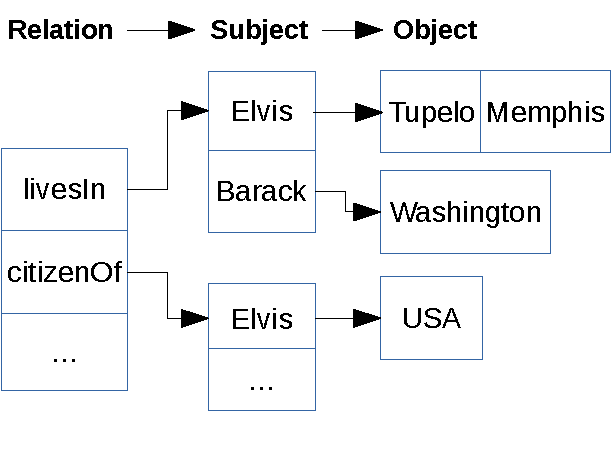
\includegraphics[width=0.5\textwidth]{figures/indexes}\
% \caption{Structure of the fact index RSO for a set of four facts}
% \label{indexes}
% \end{figure}
% 
% In addition to the fact indexes, the database relies 
% on three \emph{aggregated indexes} \texttt{S}, \texttt{P}, \texttt{O} that store the aggregated number of facts for each
% key of the fact indexes. For example, the aggregated index \texttt{P} stores the number of triples for each relation
% in the KB, e.g., $\{ livesIn=3, citizenOf=1 \}$ for the fact index depicted in Figure~\ref{indexes}. 
% Fact indexes in combination with aggregated indexes can be used to efficiently fetch the instantiations of an atom.
% They also let us determine the size of atom, i.e., its number of bindings, in constant time. 
% For example, the size of the atom $livesIn(x,y)$ can be retrieved by a simple look-up 
% in the aggregated index \texttt{P}. In constrast, the size of the atom $livesIn(x, USA)$ requires two 
% lookups in the fact index \texttt{ROS}: the first lookup to get the object values of $livesIn$ and the second
% to retrieve the list of subjects for the object value $USA$. If an atom has size greater than zero, it means
% that there exists a query answer for it in the KB.
% 
% The existence of an answer for a conjunction of atoms in a KB is described in Algorithm~\ref{exists}. 
% If the query contains a single atom (Line 3), we can directly verify if its size is greater than zero using
% the indexes (Line 4). Otherwise, we select the atom $B_s$ with fewest instantiations using the indexes (Line 6), 
% and run through all of its instantiations (Lines 8 to 13). We apply such instantiations to the remaining atoms (Line 9)
% and repeate this process recursively (Line 10) until we end up with a single atom. Since rules are connected query patterns, the atom $B_s$ must share at least
% one variable with the remaining atoms. This means that by instantiating $B_s$, some variables in the remaining atoms 
% become instantiated, making the atoms more selective with every recursive step.
% 
% \begin{algorithm}
% \caption{Checking existence}
% \label{exists}
% \begin{algorithmic}[1]
% \Function{Exists}{$B_1 \wedge ... \wedge B_n$, $\mathcal{K}$}
%     \State $q := B_1 \wedge ... \wedge B_n$
%     \If {$length(q) = 1$}
%       \State \Return size($q$, $\mathcal{K}$) $> 0$
%     \Else
%       \State $B_s := findSmallest(q, \mathcal{K})$
%       \State $q := q - \{ B_s \} $
%       \ForAll {instantiations $b_s \in B_s$}
% 	\State Replace $b_s$ in $q$
% 	  \If{Exists($q$, $\mathcal{K}$)}
% 	    \State \Return true
% 	  \EndIf
%       \EndFor
%     \EndIf
%     \State \Return false
% \EndFunction
% \end{algorithmic}
% \end{algorithm}
% 
% \paragraph{Implementation of Count-Projection Queries} Algorithm \ref{algi} shows how we answer count-projection queries
% of the form: \\ \\
% \noindent{SELECT $\bm{x}$, COUNT($H$) WHERE $H \wedge B_1 \wedge ... \wedge B_n$\\
% SUCH THAT COUNT($H$)$\geq k$} \\ \\
% These are the types of queries used to determine the relations and instances for new atoms in the specialization
% phase of AMIE. The algorithm takes as input a selection variable $\bm{x}$, a projection atom $H:=R(\bm{X},\bm{Y})$, remaining atoms $B_1, ... B_n$, 
% and a KB $\mathcal{K}$. 
% % For example, if the routine is used to find the relations for a new atom in a rule, e.g., 
% % $\bm{r}(\bm{Z}, \bm{W}) \wedge \vec{B} \Rightarrow r_h(x, y)$, then 
% % $\bm{x} = \bm{r}$, $H = r_h(x, y)$ and $\bm{r}(\bm{Z}, \bm{W}) \wedge \vec{B}$ accounts for the set $B_1, ... B_n$. 
% The algorithm returns a hash table with each instantiation of the selection variable 
% $\bm{x}$ as key and the number of distinct bindings of the projection atom $H$ as value. Notice that Algorithm~\ref{algi}
% does not consider the threshold condition (SUCH THAT) since it is actually enforced by the AMIE algorithm and not 
% the in-memory database. 
% 
% We first check whether $\bm{x}$ appears in the projection atom (Line 3).
% If that is the case (Lines 4 to 10), we run through all instantiations of the projection atom, instantiate the query accordingly (Line 6), and check for existence (Line 7).
% Each existing instantiation increases the counter for the respective value of the selection variable $\bm{x}$ (Line 8). 
% If the selection variable does not appear in the projection atom (Lines 12 to 18), 
% we iterate through all instantiations of the projection atom.
% We instantiate the query accordingly, and fire a SELECT query for $\bm{x}$ (Line 14). 
% We then increase the counter for each value of $\bm{x}$ (Line 16).
% 
% \paragraph{Implementation of Count Queries} Recall from Section~\ref{countQueries} that count queries in AMIE have the form \\ \\
% \noindent{SELECT COUNT($H'$) WHERE $H \wedge B_1 \wedge ... \wedge B_n$} \\
% 
% These queries return the number of distinct bindings of the projection atom $H$ 
% that fullfill the pattern $H \wedge B_1 \wedge ... \wedge B_n$ and are used to
% calculate the confidence of rules. Since the aggregation function COUNT conveys
% distinct semantics, the in-memory database computes a SELECT DISTINCT query 
% and then reports the size of the result set. Algorithm~\ref{select} describes
% the method to select the set of distinct bindings of the projection atom $H := r(\bm{X}, \bm{Y})$ in
% $H \wedge B_1 \wedge ... \wedge B_n$. Notice that this is not a general implementation of SELECT DISTINCT queries,
% since it is designed for binary atoms: it supports up to two variables that must occur in the same atom.
% 
% Algorithm~\ref{select} starts finding the atoms with the fewest number of instantiations $B_s$. If such atom is the
% projection atom (Lines 5 to 11), i.e., $B_s = H$, the algorithm goes through all the instantiations $h$ of the $H$, instantiates
% the query accordingly and checks whether there exists a solution for the instantiated query pattern in the KB (Line 8). 
% If it is the case, the solution $h$ is added to the result set. In contrast, if the most restrictive atom $B_s$ is not 
% the projection atom (Lines 13 to 17), the algorithm iterates through the instantiations $b_s$ and recursively 
% selects the solutions in the remaining atoms (Line 16).
% 
% \begin{algorithm}
% \caption{Select distinct}
% \label{select}
% \begin{algorithmic}[1]
% \Function{Select}{$H$, $B_1 \wedge ... \wedge B_n$, $\mathcal{K}$}
%     \State $q := H \wedge B_1 \wedge ... \wedge B_n$
%     \State $B_s := findSmallest(q)$
%     \State $result := [ ]$
%     \If{$B_s = H$}
%       \ForAll instantiations $h \in H$
% 	\State Replace $h$ in $q$
% 	\If {Exists($q$, $\mathcal{K}$)}
% 	  \State $result$.add($h$)
% 	\EndIf
%       \EndFor
%     \Else
%       \State $q := q - \{ B_s\}$
%       \ForAll{instantiations $b_s \in B_s$}
%       	\State Replace $b_s$ in $q$
%       	\State $result$.add(Select($H$, $q$, $\mathcal{K}$))
%       \EndFor
%     \EndIf
%     \State \Return $result$
% \EndFunction
% \end{algorithmic}
% \end{algorithm}
% 
% \paragraph{Summary}
% The AMIE algorithm iteratively builds more complex rules from simpler rules by the help of three operators.
% It takes advantage of monotonic measures to prune the search space efficiently and also takes care of duplicate elimination.
% We have identified projection queries as the crucial type of queries for rule mining.
% Since standard database systems and standard SPARQL systems provide no specifically tuned support for these queries,
% we have implemented a vanilla in-memory database, which has specific support for projection queries.
% Our entire implementation is in Java. The code can be downloaded from our Web site\footnote{\url{http://mpi-inf.mpg.de/departments/ontologies/projects/amie}}.
% 
% 
% \begin{algorithm}
% \caption{Answering Projection Queries}
% \label{algi}
% \begin{algorithmic}[1]
% \Function{SELECT}{$\bm{x}$, $R(X,Y) \wedge B_1 \wedge ... \wedge B_n$, $\mathcal{K}$}
%     \State $map = \{\}$
%     \State $q=B_1 \wedge ... \wedge B_n$
%     \If {$\bm{x} \in \{R,X,Y\}$}
% 	  \ForAll{instantiations $r(x,y) \in R(\bm{X}, \bm{Y})$}
% 	    \State In $q$, replace $R$ by $r$, $X$ by $x$, $Y$ by $y$
% 	    \If{Exists($q$, $\mathcal{K}$)}
% 		\State $map[x]++$
% 	    \EndIf
% 	  \EndFor
% 	\Else
% 	  \ForAll{instantiations $r(x,y) \in R(\bm{X},\bm{Y})$}
% 	    \State In $q$, replace $R$ by $r$, $X$ by $x$, $Y$ by $y$
% 	    \State $\mathcal{X} :=$ SELECT DISTINCT $\bm{x}$ FROM $\mathcal{K}$ WHERE $q$
% 	    \ForAll{$x \in \mathcal{X}$}
% 		  \State $map[x]++$
% 	    \EndFor
% 	  \EndFor
% 	\EndIf
% 	\State \Return $map$
% \EndFunction
% \end{algorithmic}
% \end{algorithm}
% \ \\[-1cm]
% }


%- - - - - - - - - - - - - - - - - - - - - - - - - - - - - -
\section{Scalability Improvements: AMIE+}
\label{sec:improvements}
Since the publication of the original AMIE framework~\cite{amie}, we have extended it with a series of improvements 
that allow the system to run over very large KBs. 
In the following, we will introduce and discuss these extensions and refer to this new version of AMIE as AMIE+.
Our extensions aim to speed up 2 different parts of the main rule-mining algorithm: (i) the refinement phase and 
(ii) the confidence evaluation. 



% Since the publication of the original AMIE framework~\cite{amie}, we have extended it with a series of improvements 
% that allow the system to run over very large KBs.
% In the following, we will introduce and discuss these extensions and refer to the extended version of AMIE as AMIE+.
% As usual when tuning a system, there are two kinds of techniques  to improve the performance:
% those that increase performance by improving the efficiency of the algorithms and those that gain efficiency at the expense of result quality.
% Hence, in the following, we first discuss  improvements over AMIE that preserve the quality of the original results and then extensions based 
% on approximations,
% which can potentially lead to a lower recall.



% \subsection{Lossless Optimizations}
% \label{prunebound}
% The techniques discussed in this subsection do not alter the output of AMIE. They include speeding up projection queries
% by means of query rewriting and caching or leveraging further constraints in the form of confidence thresholds or
% rule size limits. They allow for avoiding the execution of unnecessary queries for rules that will not be output anyway.

\subsection{Speeding Up Rule Refinement}
\label{subsec:lossless}
In this section, we will discuss how AMIE+ speeds up the rule refinement phase for specific kinds of rules.
We emphasize that the techniques described below do not alter AMIE's output in any way. 

\paragraph{Maximum Rule Length}
% \ignore{
% The maximum rule length $n$ is an input parameter for our system. AMIE stops exploring the search space as soon as all rules with a length of at most $n$ have been produced.
% In the experiments,
% we used $n=3$ though AMIE can mine longer rules. As we show later in the experimental section,
% rules with more than 3 atoms are less interesting because they often capture trivial relationships. Besides, their support tends to be very low.
% 
% For AMIE+, we improved this pruning strategy as follows.
% During the mining process, AMIE creates connected rules by applying all possible mining operators (line 9 in Algorithm~\ref{rm}) on previously created rules.
% This means that for a not-yet-closed rule of length $n-1$, AMIE applies, among others, the add-dangling-atom operator ($\mathcal{O}_D$). This results in a non-closed rule,
% which will still not be output. Since the rule has the maximum length $n$, it will not be further refined.
% Hence, the application of the operator $\mathcal{O}_D$ to open rules of size $n-1$ is useless.
% For this reason, AMIE+ refines open rules of length $n-1$ only by means of the add-closing-atom-operator ($\mathcal{O}_C$).
% }
The maximum rule length $l$ is an input parameter for our system. AMIE stops exploring the search space as soon as all rules with 
a length of at most $l$ have been produced.
% In the experiments,
% we used $n=3$ though AMIE can mine longer rules. As we show later in the experimental section,
% rules with more than 3 atoms are less interesting because they often capture trivial relationships. Besides, their support tends to be very low.
% For AMIE+, we improved this pruning strategy as follows.
During the mining process, AMIE creates connected rules by applying all possible mining operators 
(line 10 in Algorithm~\ref{rm}) on previously created rules.
Given a maximum rule length $l$ and a non-closed Horn rule of length $l-1$, AMIE+
will refine it only if it is possible to close it before exceeding the length constraint.
This means that for a not-yet-closed rule of length $l-1$, AMIE+ will not apply 
the add-dangling-atom operator $\mathcal{O}_D$, because this results in a non-closed rule,
which will be neither output nor refined. In the same spirit, if the same rule contains more than
two non-closed variables (see Section~\ref{subsec:rules}), AMIE+ will skip the application of 
the add-closing atom operator $\mathcal{O}_C$. This happens because an application of the operator 
$\mathcal{O}_C$ can close at most two variables with one atom. 
This rationale is also applicable to the add-instantiated operator $\mathcal{O}_I$:
rules with more than one non-closed variable are not refined with instantiated atoms, 
because the addition of an instantiated atom can close at most one variable.
% Since the rule has the maximum length $n$, it will not be further refined.
% Hence, the application of the operator $\mathcal{O}_D$ to open rules of size $n-1$ is useless.
% For this reason, AMIE+ refines open rules of length $n-1$ only by means of the add-closing-atom-operator ($\mathcal{O}_C$).

\paragraph{Perfect rules}
By definition, a rule cannot achieve a PCA confidence that is higher than 100\%. 
Thus, once a rule has achieved 100\% PCA confidence, we can stop adding new atoms. 
This is because the confidence cannot increase and the support can only decrease. 
Hence, any refinement is futile. We call rules with 100\% PCA confidence \emph{perfect rules}.



\paragraph{Reusing Projection Queries}
Recall from Sec.~\ref{support} that support is defined also for intermediate rules, i.e., rules that are not yet closed. 
In other words, whenever we apply an add-dangling-atom operator to a rule $R_p$ (the parent rule) to produce
a new rule $R_c$ (the child rule), the support of $R_c$ will likely be smaller than the support of $R_p$ (see the example in Sec.~\ref{support}).
However, there is one case in which the addition of a dangling atom cannot reduce the support. 
This happens when $R_c$ \comment{Chris}{@Luis: I prefer it if we define exactly when the caching can take place}
(i) already contains atoms with the same relation as the dangling atom and 
(ii) these atoms have a variable in common with the dangling atom.
An example is the parent rule $R_p:livesIn(x,y)\Rightarrow citizenOf(x,y)$ and the child rule 
$R_c: citizenOf(z,y)\wedge livesIn(x,y)\Rightarrow citizenOf(x,y)$.
Intuitively, the addition of the dangling atom $\textit{citizenOf}(z,y)$ cannot further restrict the support of $R_p$ because
the new atom is a less restrictive version of the atom $citizenOf(x,y)$.
This means that $z$ will always bind to the same values as $x$. 
From this observation, it follows that the support of $R_c$ can be rewritten as 
\begin{multline*}
supp(R_c) = \#(x,y):  citizenOf(x,y)\wedge livesIn(x,y) \\ \wedge citizenOf(x,y)
\end{multline*}
% \[
%  supp(R_c) = \#(x,y):  citizenOf(x,y)\wedge livesIn(x,y)\wedge citizenOf(x,y)
% \]
\[
 supp(R_c) = \#(x,y):   livesIn(x,y)\wedge citizenOf(x,y)
\]


%\comment{Chris}{@Luis: I prefer to keep the support formula in. It is not that the child rule can be re-written as the parent. It is the support
%of the child that is equivalent to the support of the parent.}
%\comment{Luis: I agree}


\noindent which is the same as $supp(R_p)$. Thus both $R_p$ and $R_c$ have the same support.
This observation can be leveraged to speed up projection queries.
AMIE uses projection queries during the refinement phase to choose which relations can be used to expand the rule for 
a specific operator (e.g., add-dangling-atom) and a specific binding (e.g., bind on variable $y$) \emph{such that the produced rule
passes the head coverage threshold}.
% Recall from Section~\ref{subsec:algorithm} that projection queries are used in AMIE to determine which
% relations should be used in the new atoms that will expand each rule. 
For example, for refining the example rule $R_c$ with a dangling atom joining on variable $y$, AMIE will construct the following expressions:
\[
\bm{r}(w,y) \wedge \textit{citizenOf}(z,y)\wedge \textit{livesIn}(x,y)\Rightarrow \textit{citizenOf}(x,y)
\]
\[
\bm{r}(y,w) \wedge \textit{citizenOf}(z,y)\wedge \textit{livesIn}(x,y)\Rightarrow \textit{citizenOf}(x,y)
\]
\noindent and will find the bindings of $\bm{r}$ that result in rules with support above the given threshold.
Since $R_c$ has the same support as $R_p$, we can re-use all the projection queries from $R_p$ \comment{Chris}{@Luis: I say reuse the same queries
not the query results. I.e. the queries are fired. In addition I do not say that I re-write anything because they might ask questions. The high level idea
is that you use the same queries. However I will be surprised if we save significantly with this optimization.} that bind on the 
common variables of $R_c$ and $R_p$, $x$ and $y$ in this example. Notice, though, that $R_c$
contains an additional variable, i.e., $z$ and therefore, AMIE cannot reuse the projection queries
of $R_p$ for queries that involve new atoms with the variable $z$.

% Since $R_c$ has the same support with $R_p$, all the results of the projection queries of $R_p$
% can be re-used directly (without recalculating them) by $R_c$ too. Notice, though, that since $R_c$
% contains one more variable than $R_p$ ($z$ in our example), AMIE cannot avoid firing the projection queries that involve binding new relations
% with that variable.

% Since the atom $citizenOf(z,y)$ is redundant, we can rewrite the query and omit it.
% This reduces the number of atoms of the query and therefore its running time.
% On the other hand, this technique cannot be applied when the new atoms involve the variable $z$. This happens
% because the new atoms impose extra constraints on $z$ which break the redundancy, e.g., 
% there is not guarantee anymore that $z$ always binds to the same values as $x$. For this reason, AMIE only 
% drops redundant atoms for queries where the specialization does not involve the variable in the redundant atom.


\ignore{ % Luis' version
\paragraph{Query Rewriting}

\comment{R2}{
3) Using the third optimization technique to expand a rule, AMIE+ chooses the same frequent relations for new atoms as in the last iteration when the rule is built if the rule 
is equivalent to its parent rule. The article uses an example to describe this technique, but lacks some formal definitions and discussions. 
The article should have more details to give answers to several critical questions: a) How to determine whether a new query can be rewritten to an old one? 
b) How the query rewriting is done? What rules are used in the query rewriting? c) Can this technique be applied to general rules? Or does AMIE+ only use this this technique 
for those rules that have the exact form as the given example?
}


Recall from Sec.~\ref{support} that support is defined also for intermediate rules, i.e., rules that are not yet closed. 
In other words, whenever we apply an add-dangling-atom operator to a rule $R_p$ (the parent rule) to produce
a new rule $R_c$ (the child rule), the support of $R_c$ will be likely smaller than the support of $R_p$ (see the example in Sec.~\ref{support}).
However, there is one case in which the addition of a dangling atom cannot reduce the support. 
This happens when the new atom is a less restrictive version of an existing atom in the rule.
% (i) contains a relation that already exists in the parent rule and 
% (ii) its shared variable is shared with the identical relation already existing in the rule. 
For example, imagine we specialize the rule $R_p:livesIn(x,y)\Rightarrow citizenOf(x,y)$
using the operator $\mathcal{O}_D$. One of such specializations is $R_c: citizenOf(z,y)\wedge livesIn(x,y)\Rightarrow citizenOf(x,y)$. 
The addition of the dangling atom $\textit{citizenOf}(z,y)$ cannot further restrict the support of $R_p$ because
the new atom is a less restrictive version of the atom $citizenOf(x,y)$. This means that $z$ will always 
bind to the same values as $x$. From this observation, it follows that $R_c$ can be rewritten as 
\[
R_c: citizenOf(x,y)\wedge livesIn(x,y)\Rightarrow citizenOf(x,y)
\]
\[
R_c: livesIn(x,y)\Rightarrow citizenOf(x,y)
\]

\noindent which is the same expression as the parent rule $R_p$. Thus both $R_p$ and $R_c$ have the same support.

% \ignore{
% To see why, consider the support of $R_p$:
% \[ supp(R_c) = \#(x,y): \exists z:  citizenOf(z,y)\wedge livesIn(x,y)\wedge citizenOf(x,y) \]
% Support counts only the pairs $(x,y)$, and is independend of $z$.  
% $z$ is free and can take any value, but in the most restrictive (for the support) scenario will be bound to $x$. 
% In this case, we have 
% \[
%  supp(R_c) = \#(x,y):  citizenOf(x,y)\wedge livesIn(x,y)\wedge citizenOf(x,y)
% \]
% \[
%  supp(R_c) = \#(x,y):   livesIn(x,y)\wedge citizenOf(x,y)
% \]
% 
% which is the same as $supp(R_p)$.
% }
% The fact that the addition of an atom that is almost identical (same relation, same shared variable)  to an already existing atom of the rule does not change the support of the rule 
% can also be exploited for speeding up the projection queries. 
The fact that the child rule can be rewritten into to the parent rule can be leveraged to speed up projection queries.
Recall from Section~\ref{subsec:algorithm} that projection queries are used in AMIE to determine the
relations for new atoms. Assume AMIE refines the rule $R_c$ with a dangling atom
joining on variable $y$. This implies to construct the following expressions:
\[
?r(w,y) \wedge \textit{citizenOf}(z,y)\wedge \textit{livesIn}(x,y)\Rightarrow \textit{citizenOf}(x,y)
\]
\[
?r(y,w) \wedge \textit{citizenOf}(z,y)\wedge \textit{livesIn}(x,y)\Rightarrow \textit{citizenOf}(x,y)
\]
\noindent and find the bindings of $r$ that keep their support above the given threshold.
Since the atom $citizenOf(z,y)$ is redundant, we can rewrite the query and omit it.
This reduces the number of atoms of the query and therefore its running time.
On the other hand, this technique cannot be applied when the new atoms involve the variable $z$. This happens
because the new atoms impose extra constraints on $z$ which break the redundancy, e.g., 
there is not guarantee anymore that $z$ always binds to the same values as $x$. For this reason, AMIE only 
drops redundant atoms for queries where the specialization does not involve the variable in the redundant atom.

% Intuitively, since the support of $R_c$ and $R_p$ is the same, all atoms that are good candidates (will not result in rules with support below threshold) for extending $R_p$ 
% will also be good candidates for extending $R_c$.  Therefore, if we  cache the candidates of $R_p$ we can re-use them when extending $R_c$.



 
\ignore{
In some cases, a query in the rule mining process contains redundant atoms. 
Assume, for instance, that we dequeue the intermediate non-closed rule
\indented{$citizenOf(z,y)\Rightarrow citizenOf(x,y)$}
and we want to further refine it by applying the $\mathcal{O}_D$ operator. The operator will add either $?r(w,z)$ or $?r(z,w)$ to the rule. Thus,
one of the possible count-projection queries is:
\indented{SELECT $?r$, COUNT($citizenOf(x,y)$) \\
WHERE $citizenOf(x,y) \; \wedge \; $ \\$citizenOf(z,y)\;\wedge\; ?r(w,z)$ \\
SUCH THAT COUNT($citizenOf(x,y)$)$>= k$}
Note that the atom $citizenOf(z,y)$ cannot restrict the result of the count statement any more than the atom $citizenOf(x,y)$ already does, i.e.,
if the rule  ``$\Rightarrow citizenOf(x,y)$'' has enough support to pass the threshold, so will the rule ``$citizenOf(z,y)\Rightarrow citizenOf(x,y)$''.
If we substitute $z$ with $x$ in the original query, we get:
\indented{SELECT $?r$, COUNT($citizenOf(x,y)$) \\
WHERE $citizenOf(x,y) \; \wedge \; $ \\
 $citizenOf(x,y)$ $\wedge\; ?r(w,x)$ \\
SUCH THAT COUNT($citizenOf(x,y)$)$>= k$}
which in turn can be rewritten as:
\indented{SELECT $?r$, COUNT($citizenOf(x,y)$) \\
WHERE $citizenOf(x,y) $ $\wedge\; ?r(w,x)$\\
SUCH THAT COUNT($citizenOf(x,y)$)$>= k$}
This query has already been fired in previous steps, as one of the ways to apply the operator add-dangling-atom ($\mathcal{O_D}$) to the rule
``$\Rightarrow citizenOf(x,y)$''.
%which is the projection query corresponding to the rule ``$\Rightarrow citizenOf(x,y)$''.
%Since this rule is shorter than the original rule, and since our algorithm performs a breadth first search, this query was already evaluated in a previous step.
Therefore, AMIE+ caches the results of previous queries. Whenever a new query can be rewritten into a previous one, AMIE+ reuses the result of the previous query instead of evaluating the query anew.%This means that if we cache the result of the shorter rule, we can reuse it for the longer rule.
}
}


\subsection{Speeding up Confidence Evaluation}
\label{subsec:speedingConfidenceEvaluation}
\comment{Katja}{Overall: The structure of Section~\ref{subsec:speedingConfidenceEvaluation} could be made clearer somewhere, 
e..g, Section 6.2.x provides an overview, Section 6.2... describes how to estimate xyz, etc. 
In some places it would be nice to be a bit more specific, e.g., saying explicitly how we what we mean when saying ``expensive rule''.}
\comment{Chris}{check if now better}

The calculation of the confidence scores for rules takes a significant part of the time 
of the overall rule-mining process (up to 29\% for YAGO2\comment{chris}{I do not know what is the correct number here}). 
This cost depends on the properties of each rule. The confidence calculation (both standard and PCA) involves the calculation of the 
size of the rule's body: if the body contains atoms with very selective joins, the size of the body is relatively small and the query cost remains low. 
On the other hand, if the body size is huge, it uses more resources (memory), which makes the query expensive.
Notice also that most rule mining applications are interested in rules above some confidence threshold.
For example, predictions based on rules with 1\% confidence are not useful in practice.
This means that  a rule mining system might spend a significant amount of time to evaluate expensive confidence queries only to find out that
the rule was of low confidence and of no practical use.
\ignore{
An example of such a rule that we will use also later in this section is:
\[
  directed(x,z) \wedge hasActor(z,y) \Rightarrow married(x,y)
\]

This rule concludes that a director is married to all the actors that acted in his/her movies, producing a total of 74249 married couples in YAGO2.
AMIE needs more than 500ms (more than twice the average cost: 200ms) to calculate the confidence of this intuitively bad rule.
}

% In AMIE+, we are exploiting the existence of a confidence threshold to prune rules that are ``expected'' to be ``expensive'' and 
% to have confidence lower than this threshold without actually calculating their confidence value.
In AMIE+, we use a confidence threshold in combination with a formula to approximate the confidence value 
to avoid evaluating expensive queries that would lead to low confidence rules.
Our approximation formula is based on basic statistics, such as the functionalities or the overlaps 
between domains and ranges of relations. 
These quantities
can be precomputed and can later be accessed in constant time. For example, AMIE+ prunes the example-rule above in less than 1ms.  
In addition, our approximation is designed such that it is more likely to overestimate confidence than to underestimate it.
This is important, because we use it to prune rules, and we want to avoid pruning rules that have a higher confidence in reality.
Our experiments (see Sec.~\ref{amiepm}) show that this technique can make AMIE run in the range of minutes instead of days with 4\% or less of false pruning.

In Sec.~\ref{sec:conf_appr},  we give an overview of the confidence approximation and we explain for which form of rules we use it. 
Sec.~\ref{sec:appr}, then, describes by the use of an example how the rule's body is approximated and concludes with a formula for the general case.
Sec.~\ref{sec:appr_discussion} discusses the underlying assumptions made by our approximation and explains how it is used within AMIE+. 
Finally, Sec.~\ref{sec:conf_upperBounds} derives upper bounds for the confidence of rules of a more specific form.





% Most rule mining applications have no use for rules with low confidence. 
% For example, predictions based on rules with 1\% confidence are not useful in practice.
% Based on this observation, AMIE accepts a minimum confidence threshold for both the PCA and the standard confidence. However,
% due to the non-monotonic behavior of the confidence metrics, Algorithm~\ref{rm} does not use these thresholds for pruning.
% Hence, in AMIE, pruning based on confidence thresholds is applied only directly before the rules are output. Consequently, only the output is influenced, not the runtime.

% For AMIE+, we have developed a way to use minimum confidence thresholds to improve the performance of the system.  
% We use the confidence threshold in combination with a formula to approximate the confidence value 
% to avoid evaluating expensive queries that would lead to low confidence rules.
% In the following, we discuss how to approximate confidence  for ``potentially expensive'' rules. 
% Our approximation formula is based on simple statistics, such as the functionalities or the overlaps between domains and ranges of various relations. 
% These quantities
% can be precomputed and can later be accessed in constant time. In addition, our approximation is designed such that it is more likely to overestimate confidence than to underestimate it.
% This is important, because we use it to prune rules, and we want to avoid pruning rules that have a higher confidence in reality.
% Our experiments (see Sec.~\ref{amiepm}) show that this technique can make AMIE run in the range of minutes instead of days with 4\% or less of false pruning.


\subsubsection{Confidence Approximation}\label{sec:conf_appr}

\comment{Katja}{For ease of reading, it might be useful to also repeat what the variables represent.}
By the time AMIE has to calculate the confidence of a rule, the system already knows the support of the rule.
Recall that confidence and PCA confidence (see Sections~\ref{subsubsec:stdConf} and \ref{subsubsec:pcaConf}) are defined as:
\[conf(\vec{B} \Rightarrow r_h(x,y)) := \frac{supp(\vec{B} \Rightarrow r_h(x,y))}{\#(x,y): \exists z_1,...,z_m: \vec{B}}\]
and
\begin{multline*}
conf_{pca}(\vec{B} \Rightarrow r_h(x,y)) :=\\
\frac{supp(\vec{B} \Rightarrow r_h(x,y))}{\#(x,y): \exists z_1,...,z_m,y': \vec{B} \wedge r_h(x,y')}
\end{multline*}
\noindent Given that support is known, the remaining step is to fire the queries for the denominators of the confidence expressions
(see Sections~\ref{subsubsec:stdConf} and \ref{subsubsec:pcaConf}), denoted as $dnm_{std}$ and $dnm_{pca}$:
\begin{equation} \label{eq:denomStandardConf}
 dnm_{std}(\vec{B} \Rightarrow r_h(x,y)):= \#(x,y): \exists z_1,...,z_m: \vec{B}
\end{equation}
and
\begin{equation} \label{eq:denomPCA}
\begin{array}{rl}
dnm_{pca}(\vec{B} \Rightarrow r_h(x,y)) := {}& \#(x,y): \exists z_1,...,z_m,y': \\ &\quad \vec{B} \wedge r_h(x,y')
\end{array}
\end{equation}



Our aim is to derive a conservative approximation for $dnm_{pca}$ (or $dnm_{std}$) denoted by
$\widehat{dnm}_{pca}$. By plugging this expression into the confidence formula, we get
\begin{equation} \label{eq:pcaApproxConf}
  \widehat{conf}_{pca}(R):=\frac{supp(R)}{\widehat{dnm}_{pca}(R)}
\end{equation}

Let us re-consider Eq.~\ref{eq:denomPCA}:
\[
\begin{array}{rl}
 dnm_{pca}(\vec{B}(x,y) \Rightarrow r_h(x,y)) := {} \#(x,y): \exists z_1,...,z_m,y': \\ \quad \vec{B}(x, y) \wedge r_h(x,y')
\end{array}
\]
Here we resort to an abstraction that treats the body of the rule $\vec{B}(x, y)$ as a relation on the head variables. 
% If $\vec{B}$ has functionality $fun(\vec{B})$, it means that for each entity in variable $x$ (``domain'' of $\vec{B}$) the body will produce $1/fun(\vec{B})$ entities in $y$,
% i.e., the body produces $\#y_{per\; x} = 1/fun(\vec{B})$ facts per entity in its ``range'', on average. If we multiply this number
% by the number of entities that bind to $x$, we obtain an estimate for the body size of the rule. 
If $\vec{B}$ has functionality $fun(\vec{B})$, it means that, on average, each entity in variable $x$ 
relates to $\#y_{per\; x} = 1/fun(\vec{B})$ bindings in $y$. If we denote the domain and range of a relation $r$ as
$dom(r)$ and $rng(r)$ respectively, the expression $\#y_{per\; x} \times |dom(\vec{B})|$ gives us 
an estimate for the body size of the rule. 
However, for the PCA confidence, the denominator is restricted also by the entities in the domain of the head relation.
This consideration leads us to the expression:
% If we denote with $|dom(r)|$ the number of entities in the domain of relation $r$, our approximation has the form:
\begin{equation} \label{eq:pcaApproxConf_general}
  \widehat{dnm}_{pca}(R):=|dom(\vec{B}) \cap dom(r_h)|\cdot \#y_{per\; x}
\end{equation}

% % Notice that we are trying to approximate the number of entities produced in the place of the less functional variable $y$ for each entity in the place of the most functional variable $x$.
% %In the following we will show how to approximate the quantities $\#y_{per\; x}$ and $dom(\vec{B})$.
% In the following, we discuss how to calculate the terms of this expression in an efficient way. 
% Additionally, we show how this approximation can help AMIE spot low confident rules for which the confidence
% calculation is very expensive. As our experimental results show, this reduces runtime significantly 
% as it avoids investing resources in expensive rules that will not be output otherwise.


In the following, we first describe for which kind of rules it makes sense to use this approximation and then, in Sec.~\ref{sec:appr}, 
we discuss how to calculate the terms of Eq.~\ref{eq:pcaApproxConf_general} in an efficient way. 


\paragraph{When to use a confidence approximation}\label{sec:expensive_rules}
Using any form of confidence approximation  always involves the risk of pruning a good rule. 
At the same time, if the rule's exact confidence is cheap to compute, the potential gain of using an approximation is small.
For this reason, we only use the confidence approximation for rules, whose exact confidence is relatively ``expensive'' to compute.
% Recall that using a confidence approximation to prune rules is worth only if the exact confidence calculation is expensive. 
% If it is not the case, the gain in runtime becomes small at the risk of unnecessary pruning.
% Therefore we only use the confidence approximation for ``expensive'' rules. 
These rules typically have a large number of bindings in the body, which translates into 
higher runtimes and memory usage. An example is the rule 
\[
 directed(x,z) \wedge hasActor(z,y) \Rightarrow married(x,y)
\]

This rule concludes that a director is married to all the actors that acted in his/her movies, producing a total of 74249 married couples in YAGO2.
AMIE needs more than 500ms (more than twice the average cost: 200ms) to calculate the confidence of this intuitively bad rule.



This phenomenon mainly occurs in expressions that contain existentially quantified variables in Eq.~\ref{eq:denomPCA}, 
because such variables introduce many intermediate results. In our example
rule, a director $x$ is related to many movies $z$ (the intermediate variable) that have different actors. 
In AMIE+, we define as \emph{expensive} rules, rules whose bodies (i) contain variables other than the variables appearing in the head atom ($z$ in our example) and
(ii) if these additional variables define a single path between the head variables ($x \rightarrow z \rightarrow y$ in our example).


We therefore use the confidence approximation only for rules for which the $x,y$ head-variables are connected through a single 
chain of existentially quantified variables $z_1,..., z_{n-1}$. These rules have the form:
$$
  r_1(x,z_1) \wedge r_2(z_1,z_2) \wedge ... \wedge r_n(z_{n-1},y) \Rightarrow r_h(x,y)
$$

Notice that in order to write a rule in this canonical form we may need to replace some relations by their inverses
(e.g., substitute $r_2(z_2,z_1)$ with $r_2^{-1}(z_1,z_2)$)
and change the order of the atoms.

In contrast, rules that do not contain existential variables (e.g., $livesIn(x,y)\wedge bornIn(x,y)\Rightarrow diedIn(x,y)$)  
or that contain multiple paths between the head variables (e.g. $livesIn(x,z_1)\wedge locatedIn(z_1,y)\wedge bornIn(x,z_2)\wedge locatedIn(z_2,y) \Rightarrow isCitizenOf(x,y)$)
are usually associated with more selective queries. In our examples both $livesIn$ and $bornIn$ join on $x$ in the body and restrict the result-size.


In the following, we first explain how to compute the approximation for the case of a single 
path with one existential variable through a running example.
Then we generalize to rules with many existential variables, forming a single path. 

% \comment{Katja}{The following paragraph is not well connected, e.g., dnm is mentioned nowhere else in this subsubsection}
% \comment{chris}{took all formulas out. Just say we do not approximate}
% If there are $m$ paths connecting $x$ and $y$, AMIE does not make use the approximation formula. The reason for this is that the $dnm$
% for the combination of all paths will be smaller than the $dnm$ for each individual path. 
% In other words, we neither expect such rules to have large bodies nor to be particularly expensive in terms of confidence computation.


% If there are $m$ paths connecting $x$ and $y$, we can compute, the support and confidence denominator for each path separately.
% The quantity $\#y_{per\;x}$ (and the support) for the combination of all paths can be upper-bounded by the minimum of the $\#y_{per\;x}$ (and the support respectively) 
%  of all individual paths \comment{Luis}{This part is not clear. You are suggesting the minimum of which expression exactly?}\comment{chris}{now?}. 
% Our confidence approximation will then be:
% 
% \[
%  \widehat{conf}_{pca} =\frac{min(supp_1,supp_2,...,supp_{m})}{min(\widehat{dnm}_1,\widehat{dnm}_2,...,\widehat{dnm}_m)}
% \]
% 
% where $supp_i$ and $\widehat{dnm}_i$ are the support and the denominator approximation of path $i$.
% Notice that the denominator of the above formula is only an upper bound for the real denominator. 
% However, the existence of multiple paths makes always the denominator query more selective and therefore not as expensive (similar to the case of the 
% example $livesIn(x,y)\wedge bornIn(x,y)\Rightarrow diedIn(x,y)$). Since the benefit from using the approximation formula for multiple-path-rules
% is expected to be limited in comparison to the risk of false pruning, we only use the approximation formula for single-path rules. 
% \comment{Luis}{This part I do not get either.}


\subsubsection{Approximating the Confidence Denominator} \label{sec:appr}
In the following, we denote the domain and range of $r$ with $dom(r)$ and $rng(r)$, respectively.
In addition, we use the shortcut notation $ov_{dr}(r_1,r_2)$, $ov_{rd}(r_1,r_2)$, $ov_{dd}(r_1,r_2)$, $ov_{rr}(r_1,r_2)$
for the size of the overlap sets between the domains and ranges 
of pairs of relations, e.g., $ov_{dr}(r_1,r_2) := |dom(r_1) \cap rng(r_2)|$.
Let us now consider again the rule
\[
 directed(x,z) \wedge hasActor(z,y) \Rightarrow married(x,y)
\]
which implies that a director is married to all actors that acted in his movies.
Recall that the calculation of $dnm_{pca}(R)$ is defined by the expression:
\[
\begin{array}{rl}
dnm_{pca}(R) := &\#(x,y): \exists\; z, y': directed(x,z)  \\
  &\wedge\; hasActor(z,y) \wedge isMarried(x,y') \label{eq:denomPCAExample}
\end{array}
\]
Here $\vec{B}(x, y) = directed(\bm{x},z) \wedge hasActor(z,\bm{y})$.
To calculate the approximation defined in Equation~\ref{eq:pcaApproxConf_general}, 
we need to calculate the number of directors in $\vec{B}$ that are married, i.e.,  
$|dom(\vec{B})\;\cap\;dom(isMarried)|$ and the number of actors $y$ 
associated to each director $x$, i.e.,$\#y_{per\;x}$.
We focus on the latter term. 
This requires us to walk from the most to the least functional variable, i.e., through the path $x \rightarrow z \rightarrow y$, connecting a director to his potential actors. 
If $fun(r)$ and $ifun(r)$
denote the functionality and inverse functionality of the relation $r$, respectively, then
walking through this path involves the following steps:
\begin{enumerate} \itemsep +0.3ex
 \item For each director $x$, the relation $directed$ will produce on average $\frac{1}{fun(directed)}$ movies $z$.
 \item Some or all of these movies $z$ will find join partners in the first argument of $hasActor$.
 \item For each movie $z$, $hasActor$ will produce on average $\frac{1}{fun(hasActor)}$ actors $y$.
 \item Each of these actors in $y$ acted on average in  $\frac{1}{ifun(hasActor)}$ movies of the $hasActor$ relation.
\end{enumerate}
Up to step 2, we can approximate the number of distinct movies that bind to the variable $z$ for each director in the variable $x$ as:
$$
\#z_{per \; x} := \frac{ ov_{rd}(directed,hasActor) }{|rng(directed)| \times fun(directed)}
$$
Here, $|rng(directed)|$ is the number of distinct movies in the range of $directed$ and $ov_{rd}(directed,hasActor)$ 
denotes the distinct movies in the overlap between the objects of $directed$ and the subjects of $hasActor$.
The term $\frac{1}{fun(directed)}$ corresponds to step  1.
Our join estimation assumes that the movies in the overlap of $directed$ 
and $hasActor$ are uniformly distributed between the different directors in $directed$.

For steps 3 and 4, we can approximate the number of actors in the variable $y$ for each movie in the variable $z$ as follows:
$$
\#y_{ per \; z} := \frac{ifun(hasActor)}{fun(hasActor)}
$$
The term $\frac{1}{fun(hasActor)}$ corresponds to step 3. At the end of this step, 
we already have for a single director in $x$, a bag of actors in $y$ that correspond to it.
However, these are not necessarily distinct actors, since $x$ and $y$ are connected through the variable $z$ (movies). Therefore, a duplicate elimination step is needed.
To see why, assume that each director has directed on average 3 movies and that each movie has 5 actors. Then, the rule will produce on average 15 actors $y$ for each director $x$.
However, there is no guarantee that these actors are distinct.
If the director trusts specific actors and collaborates repeatedly with them in some or all of his movies, there will be less than 15 distinct actors.
% The term $\frac{1}{ifun(hasActor)}$ achieves this duplicate elimination: each actor contributes in the final count 
% with a weight $ifun(hasActor)$, 
% which expresses the extend to which this actor exclusively belongs to a movie.
The term $ifun(hasActor)$ achieves this duplicate elimination: 
since each actor participated in $\frac{1}{ifun(hasActor)}$ different movies, then the actor
contributes in the final count with a weight that is inversely proportional to this number.


From our way of performing duplicate elimination, a single actor $y$ belongs to $\frac{1}{ifun(hasActor)}$ different movies $z$, 
which are chosen from \emph{all} the movies in the relation $hasActor$.
%(e.g., 3 movies per actor).
% In reality, we want the number of different movies chosen from those that remain after step 2 ($\#z_{per \; x}$),
% i.e., the average number of movies by the same director that an actor acts in (e.g., 2 movies per actor, which is less than 3).
% In other words, in step 4, we employ a very pessimistic scenario, which causes $\#y_{per\;x}$ to be an underestimation, 
% and the overall confidence approximation to be an overestimation of the actual confidence.
In reality, we want the number of different movies chosen from those that remain after step 2, % that correspond to the same $x_2$,
i.e., the average number of movies by the same director that an actor acts in. This number is obviously smaller, which
implies that the factor $ifun(hasActor)$ is a pessimistic estimator. This makes 
our approximation an underestimation of the real confidence denominator, 
and the overall confidence approximation an overestimation of the actual confidence.

With all that said, we can estimate the number of actors $y$ that are supposed to be married with each director $x$ as:
$$
 \#y_{per\;x} :=  \#z_{per \; x} \times \#y_{ per \; z}
$$
\noindent To calculate $\widehat{dnm}_{pca}$ from Equation.~\ref{eq:pcaApproxConf_general}, we are now only missing 
the expression $|dom(\vec{B})\;\cap\;dom(isMarried)|$. 
Here we make the simplifying assumption that $dom(\vec{B}) = dom(directed)$, so that the expression
becomes the size of the join between the relations $directed$ and $married$, on the subject argument, 
that is $ov_{dd}(directed,married)$.

To summarize, the $ \widehat{dnm}_{pca}(R)$ for a rule $r_1(x,z)\wedge r_2(z,y) \Rightarrow r_h(x,y)$ can be approximated by:
\[
  \widehat{dnm}_{pca}(R) := \frac{ov_{dd}(r_1,r_h) \cdot ov_{rd}(r_1,r_2) \cdot ifun(r_2)  }{fun(r_1) \cdot |rng(r_1)| \cdot fun(r_2)}
\]
For the more general case of a rule that contains $n-1$ existential variables forming a single path from $x$ to $y$
$$
  r_1(x,z_1) \wedge r_2(z_1,z_2) \wedge ... \wedge r_n(z_{n-1},y) \Rightarrow r_h(x,y)
$$

\noindent the formula becomes:

\begin{eqnarray*}
  \widehat{dnm}_{pca}(R) := \frac{ov_{dd}(r_1,r_h)}{fun(r_1)}  \times 
  \prod_{i=2}^{n}\frac{ov_{rd}(r_{i-1},r_i) }{|rng(r_{i-1})|}\frac{ifun(r_i)}{fun(r_i)}
\end{eqnarray*}





%%%%%%%%%%%%%%%%%%%%%%%%%%%%%%%%%%%%%%%%%%%%%%%%%%%%%
\ignore{
\subsubsection{Confidence Upper Bounds}
\label{upperBound}

\comment{R2}{
4) The fourth optimization technique uses a confidence threshold to filter out generated closed rules that have a small confidence upper bound to avoid expensive computations for its actual confidence. 
This technique can only be used for rules with exactly two body atoms of the same predicate sharing one variable. 
This restriction limits the benefits gained from applying this technique. 
As shown in Table 7 in the experiments section, we can see that there is not a big improvement in execution time and only a small amount of rules may be removed.
}

\paragraph{Confidence Thresholding}
Most rule mining applications have no use for rules with low confidences. For example, predictions based on rules with 1\% confidence are not useful in practice.
Based on this observation, AMIE+ accepts a minimum confidence threshold for both the PCA and the standard confidence. However,
due to the non-monotonic behavior of the confidence metrics, Algorithm~\ref{rm} does not use these thresholds for pruning.
Hence, in AMIE, pruning based on confidence thresholds is applied only directly before the rules are output. Consequently, only the output is influenced, not the runtime.


\paragraph{Pruning} 
For AMIE+, we have developed a way to use minimum confidence thresholds to improve the performance of the system.  
We use the confidence threshold to avoid evaluating expensive queries that would lead to low confidence rules.
%As we have already discussed in Algorithm~\ref{rm} (line 6), AMIE adds a rule in the result set only if this rule has a confidence value above the confidence threshold.
By the time AMIE has to calculate the confidence of a rule, the system already knows the support of the rule.
Recall that confidence and PCA confidence (see Sections~\ref{subsubsec:stdConf} and \ref{subsubsec:pcaConf}) are defined as:
\[conf(\vec{B} \Rightarrow r(x,y)) := \frac{supp(\vec{B} \wedge r(x,y))}{\#(x,y): \exists z_1,...,z_m: \vec{B}}\]
and
\begin{multline*}
conf_{pca}(\vec{B} \Rightarrow r(x,y)) :=\\
\frac{supp(\vec{B} \wedge r(x,y))}{\#(x,y): \exists z_1,...,z_m,y': \vec{B} \wedge r(x,y')}
\end{multline*}
\noindent Given that support is known, the remaining step is to fire the queries for the denominators of the confidence expressions
(see Sections~\ref{subsubsec:stdConf} and \ref{subsubsec:pcaConf}), denoted as $dnm_{std}$ and $dnm_{pca}$:
\begin{equation} \label{eq:denomStandardConf}
 dnm_{std}(\vec{B} \Rightarrow r(x,y)):= \#(x,y): \exists z_1,...,z_m: \vec{B}
\end{equation}
and
\begin{equation} \label{eq:denomPCA}
\begin{array}{rl}
dnm_{pca}(\vec{B} \Rightarrow r(x,y)) := {}& \#(x,y): \exists z_1,...,z_m,y': \\ &\quad \vec{B} \wedge r(x,y')
\end{array}
\end{equation}

\noindent In some cases, such queries are very expensive and have a great impact on the overall running time. As an example,
consider the low confidence rule R: \[citizenOf(x,z)\:\wedge\:citizenOf(y,z) \Rightarrow married(x,y)\]
It implies that people of the same citizenship are all married to each other.
The corresponding denominator expressions for the standard confidence (Equation~\ref{eq:denomStandardConf}) and the PCA confidence (Equation~\ref{eq:denomPCA}) are:
\begin{equation*}
\begin{array}{rl}
dnm_{std}(R) := & \#(x,y): \exists z: citizenOf(x,z)\\ & \wedge\; citizenOf(y,z)
\end{array}
\label{eq:denomStandardCofn}
\end{equation*}
\begin{equation*}
\begin{array}{rl}
dnm_{pca}(R) := &\#(x,y): \exists z, y': citizenOf(x,z)  \\
  &\wedge\; citizenOf(y,z) \wedge isMarried(x,y') \label{eq:denomPCA}
\end{array}
\end{equation*}

These values are very large and therefore expensive to calculate. Besides, it is obvious that the example rule has low quality, and
that it will be filtered out in the sequel by any reasonable confidence threshold.

In the following, we devise an upper bound to prune expensive and low quality rules without having to evaluate their exact confidences.
Consider rules of the forms
$$ r(x,z) \wedge r(y,z) \Rightarrow r_h(x,y) $$
$$ r(z,x) \wedge r(z,y) \Rightarrow r_h(x,y) $$
For the sake of brevity, we will derive confidence bounds for the first form of rules as the process is analogous for the second case.
To calculate the standard confidence of our rules, we need to divide the support by the expression:
$$
dnm_{std} := \#(x,y): \exists z: r(x,z) \wedge r(y,z)
$$
Since both atoms contain the same relation, we know that all the entities of $z$ in the first atom
will join with the second atom. Furthermore,
we know that the join will result in \emph{at least} one $y$-value for each binding of $x$, i.e., the case where $y=x$. This allows us to rewrite
the expression as
$$
dnm_{std} \ge \#(x,x): \exists z:  r(x,z) \wedge r(x,z)
$$
which can be further simplified into:
\begin{equation}
 dnm_{std} \ge \#x: \exists z:  r(x,z)  \label{eq:stdBoundDenom}
\end{equation}
This expression can be calculated in constant time with the indexes of our in-memory database (see Section~\ref{subsec:implementation} for more details on the in-memory database).
%\comment{Katja}{Reference to section that explains why?} \comment{Luis}{What do you think now? We may have to detail Section~\ref{subsec:implementation} a little bit more}
%\comment{Katja}{If we state here that some indexes do the trick for us, we need to explain somewhere what indexes these are, either here here or in another section. Depends on how ``complicated'' the indexes are.}
% Fabian: This query and the indexes are trivial
The same rationale can be applied to the denominator of the PCA confidence
$$
dnm_{pca} := \#(x,y): \exists z, y': r(x,z) \wedge r(y,z) \wedge r_h(x,y)
$$
This implies
\begin{equation} \label{eq:pcaBoundDenom}
dnm_{pca} \ge \#x: \exists \;z, y': r(x,z) \wedge r_h(x,y')
\end{equation}
Although this expression requires to fire a query, it contains fewer atoms than the original expression and counts instances
of a single variable instead of pairs. It is therefore much cheaper than the original query.

Both Inequalities \ref{eq:stdBoundDenom} and \ref{eq:pcaBoundDenom}
define lower bounds for the number of pairs in the denominator expressions of the standard
and the PCA confidence, respectively. Thus, they constitute hard upper bounds for these scores.
AMIE+ first checks if an upper bound can be computed for the rule. If so, it computes the bound according to Inequality~\ref{eq:pcaBoundDenom}.
If the bound is below the confidence threshold, it reports the upper bound as confidence value and the calculation of the exact confidence according to Equation~\ref{eq:pcaConf} is skipped.
Otherwise, it calculates confidence as in Equation~\ref{eq:pcaConf} and returns the result.


%%%%%%%%%%%%%%%%%%%%%%%%%%%%%%%%%%%%%%%%%%%%%%%%%%%%%%%%%%%%%%%%%%%%%%%%%%%%%%%%%%%%%%%%%%%%%%%%%%%
%%%%%%%%%%%%%%%%%%%%%%    Pruning by approximation    %%%%%%%%%%%%%%%%%%%%%%%%%%%%%%%%%%%%%%%%%%%%%%%%%%
%%%%%%%%%%%%%%%%%%%%%%%%%%%%%%%%%%%%%%%%%%%%%%%%%%%%%%%%%%%%%%%%%%%%%%%%%%%%%%%%%%%%%%%%%%%%%%%%%%%
\subsection{Pruning by Approximation}
\label{subsec:pruningbyapprox}


The bound for the confidence that we derived in Section~\ref{upperBound} is applicable only when the same relation appears twice in the body.
In the following, we show how to approximate confidence for rules of a more general form. 
Our approximation formula is based on simple statistics, such as the functionalities or the overlaps between domains and ranges of various relations. These quantities
can be precomputed and can later be accessed in constant time. In addition, our approximation is designed such that it is more likely to overestimate confidence than to underestimate it.
This is important, because we use it to prune rules, and we want to avoid pruning rules that have a higher confidence in reality.
Our experiments (see Sec.~\ref{amiepm}) show that this technique can make AMIE run in the range of minutes instead of days with 4\% or less of false pruning.

Since support is calculated early in the process for each rule $R$ (for pruning purposes), 
our aim is to derive a conservative approximation for $dnm_{pca}$ (or $dnm_{std}$) denoted by
$\widehat{dnm}_{pca}$. By plugging this expression into the confidence formula, we get
\begin{equation} \label{eq:pcaApproxConf}
  \widehat{conf}_{pca}(R):=\frac{supp(R)}{\widehat{dnm}_{pca}(R)}
\end{equation}

Let us re-examine Eq.~\ref{eq:denomPCA}:
\[
\begin{array}{rl}
 dnm_{pca}(\vec{B}(x,y) \Rightarrow r(x,y)) := {} \#(x,y): \exists z_1,...,z_m,y': \\ \quad \vec{B}(x, y) \wedge r_h(x,y')
\end{array}
\]
Here we resort to an abstraction that treats the body of the rule $\vec{B}(x, y)$ as a relation
on the head variables. If $\vec{B}$ has functionality $fun(\vec{B})$, it means that for each entity in variable $x$ (``domain'' of $\vec{B}$) the body will produce $1/fun(\vec{B})$ entities in $y$,
i.e., the body produces $\#y_{per\; x} = 1/fun(\vec{B})$ facts per entity in its ``range'', on average. If we multiply this number
by the number of entities that bind to $x$,
we obtain an estimate for the body size of the rule. However, for the PCA confidence, the denominator is restricted also by the entities in the domain of the head relation.
If we denote with $|dom(r)|$ the number of entities in the domain of relation $r$, our approximation has the form:
\begin{equation} \label{eq:pcaApproxConf_general}
  \widehat{dnm}_{pca}(R):=|dom(\vec{B}) \cap dom(r_h)|\cdot \#y_{per\; x}
\end{equation}
% In the above formula,
% the critical terms are $dom(\vec{B})$ and $\#y_{per\; x}$.
% These are the expressions that we would like to approximate.
Recall that using a confidence approximation to prune rules is worth only if 
the exact confidence calculation is expensive. 
If it is not the case, the gain in runtime becomes small at the risk of unnecessary pruning.
Therefore we only use the confidence approximation for ``expensive'' rules. 
These rules typically have a large number of bindings in the body, which translates into 
higher runtimes and memory usage. An example is the rule 
\[
 directed(x,z) \wedge hasActor(z,y) \Rightarrow married(x,y)
\]
This rule concludes that a director is married to all the actors that acted in his movies. Its
confidence is low because the number of bindings in the body is very large. 
This phenomenon mainly occurs in expressions that contain existentially quantified variables in Eq.~\ref{eq:denomPCA}, 
$z$ in this example. This happens because such variables introduce many intermediate results. In our example
rule, a director is related to many movies. In contrast, if a rule does not contain additional variables, 
e.g., $livesIn(x,y)\wedge bornIn(x,y)\Rightarrow diedIn(x,y)$, the query associated to it becomes very selective.
% it can only further restrict the number of $(x,y)$ pairs produced by the body.
% For example, the body of the rule $livesIn(x,y)\wedge bornIn(x,y)\Rightarrow diedIn(x,y)$ has fewer or the same number 
% of bindings than the rule $bornIn(x,y)\Rightarrow diedIn(x,y)$.

We therefore focus on rules for which the $x,y$ variables are connected through a single 
chain of existentially quantified 
variables $z_1,..., z_{n-1}$. These rules have the form:
$$
  r_1(x,z_1) \wedge r_2(z_1,z_2) \wedge ... \wedge r_n(z_{n-1},y) \Rightarrow r_h(x,y)
$$

Notice that in order to write a rule in this form we may need to replace some relations by their inverses
(e.g., substitute $r_2(z_2,z_1)$ with $r_2^{-1}(z_1,z_2)$)
and change the order of the atoms.
In the following, we first explain how to compute the approximation for the case of a single 
path with one existential variable through a running example.
Then we generalize to rules with many existential variables, forming a single path and, 
in the end, we discuss the case of multiples paths.


\subsubsection{Approximate Confidence Denominator}
Let us consider again the rule
\[
 directed(x,z) \wedge hasActor(z,y) \Rightarrow married(x,y)
\]
which implies that a director is married to all actors that acted in his movies.
Recall that the calculation of $dnm_{pca}(R)$ is defined by the expression:
\[
\begin{array}{rl}
dnm_{pca}(R) := &\#(x,y): \exists\; z, y': directed(x,z)  \\
  &\wedge\; hasActor(z,y) \wedge isMarried(x,y') \label{eq:denomPCAExample}
\end{array}
\]
Here $\vec{B}(x, y) = directed(\bm{x},z) \wedge hasActor(z,\bm{y})$.
To calculate the approximation defined in Equation~\ref{eq:pcaApproxConf_general}, 
we need to calculate the number of directors in $\vec{B}$ that are married, i.e.,  
$|dom(\vec{B})\;\cap\;dom(isMarried)|$ and the number of actors $y$ 
associated to each director $x$, i.e.,$\#y_{per\;x}$.
%We need to find out how many actors correspond to each director ($\#y_{per\;x}$) in the body of the rule.
We focus on the latter term. This requires us to walk through the path $x \rightarrow z \rightarrow y$, connecting a director to his potential actors. If $fun(r)$ and $ifun(r)$
denote the functionality and inverse functionality of the relation $r$, respectively, then
walking through this path involves the following steps:
\begin{enumerate} \itemsep +0.3ex
 \item For each director $x$, the relation $directed$ will produce on average $\frac{1}{fun(directed)}$ movies $z$.
 \item Some or all of these movies $z$ will find join partners in the first argument of $hasActor$.
 \item For each movie $z$, $hasActor$ will produce on average $\frac{1}{fun(hasActor)}$ actors $y$.
 \item Each of these actors in $y$ acted on average in  $\frac{1}{ifun(hasActor)}$ movies of the $hasActor$ relation.
\end{enumerate}

Up to step 2, we can approximate the number of distinct movies that bind to the variable $z$ for each director in the variable $x$ as:
$$
\#z_{per \; x} := \frac{|rng(directed) \cap dom(hasActor)|}{|rng(directed)| \times fun(directed)}
$$
Here, $|rng(directed)|$ is the number of distinct movies in the range of $directed$ and $|rng(directed) \cap dom(hasActor)|$ 
denotes the distinct movies in the overlap between the objects of $directed$ and the subjects of $hasActor$.
The term $\frac{1}{fun(directed)}$ corresponds to step  1.
Our join estimation assumes that the movies in the overlap of $directed$ 
and $hasActor$ are uniformly distributed between the different directors in $directed$.

For steps 3 and 4, we can approximate the number of actors in the variable $y$ for each movie in the variable $z$ as follows:
$$
\#y_{ per \; z} := \frac{ifun(hasActor)}{fun(hasActor)}
$$
The term $\frac{1}{fun(hasActor)}$ corresponds to step 3. At the end of this step, 
we already have for a single director in $x$, a bag of actors in $y$ that correspond to it.
However, these are not necessarily distinct actors, since $x$ and $y$ are connected through the variable $z$ (movies). Therefore, a duplicate elimination step is needed.
To see why, assume that each director has directed on average 3 movies and that each movie has 5 actors. Then, the rule will produce on average 15 actors $y$ for each director $x$.
However, there is no guarantee that these actors are distinct.
If the director trusts specific actors and collaborates repeatedly with them in some or all of his movies, there will be less than 15 distinct actors.



% The term $\frac{1}{ifun(hasActor)}$ achieves this duplicate elimination: each actor contributes in the final count 
% with a weight $ifun(hasActor)$, 
% which expresses the extend to which this actor exclusively belongs to a movie.
The term $ifun(hasActor)$ achieves this duplicate elimination: 
since each actor participated in $\frac{1}{ifun(hasActor)}$ different movies, then the actor
contributes in the final count with a weight that is inversely proportional to this number.


From our way of performing duplicate elimination, a single actor $y$ belongs to $\frac{1}{ifun(hasActor)}$ different movies $z$, 
which are chosen from \emph{all} the movies in the relation $hasActor$.
%(e.g., 3 movies per actor).
% In reality, we want the number of different movies chosen from those that remain after step 2 ($\#z_{per \; x}$),
% i.e., the average number of movies by the same director that an actor acts in (e.g., 2 movies per actor, which is less than 3).
% In other words, in step 4, we employ a very pessimistic scenario, which causes $\#y_{per\;x}$ to be an underestimation, 
% and the overall confidence approximation to be an overestimation of the actual confidence.
In reality, we want the number of different movies chosen from those that remain after step 2, % that correspond to the same $x_2$,
i.e., the average number of movies by the same director that an actor acts in. This number is obviously smaller, which
implies that the factor $ifun(hasActor)$ is a pessimistic estimator. This makes 
our approximation an underestimation of the real confidence denominator, 
and the overall confidence approximation an overestimation of the actual confidence.

With all that said, we can estimate the number of actors $y$ that are supposed to be married with each director $x$ as:
$$
 \#y_{per\;x} :=  \#z_{per \; x} \times \#y_{ per \; z}
$$
\noindent To calculate $\widehat{dnm}_{pca}$ from Equation.~\ref{eq:pcaApproxConf_general}, we are now only missing 
the expression $|dom(\vec{B})\;\cap\;dom(isMarried)|$. 
Here we make the simplifying assumption that $dom(\vec{B}) = dom(directed)$, so that the expression
becomes the size of the join between the relations $directed$ and $married$, on the subject argument.

To summarize, the $ \widehat{dnm}_{pca}(R)$ for a rule $r_1(x,z)\wedge r_2(z,y) \Rightarrow r_h(x,y)$ can be approximated by:
\[
  \widehat{dnm}_{pca}(R) := \frac{|dom(r_1) \cap dom(r_h)| \cdot |rng(r_1) \cap dom(r_2)| \cdot ifun(r_2)  }{fun(r_1) \cdot |rng(r_1)| \cdot fun(r_2)}
\]
For the more general case of rule that contains $n-1$ existential variables forming a single path from $x$ to $y$
$$
  r_1(x,z_1) \wedge r_2(z_1,z_2) \wedge ... \wedge r_n(z_{n-1},y) \Rightarrow r_h(x,y)
$$

\noindent the formula becomes:

\begin{eqnarray*}
  \widehat{dnm}_{pca}(R) := \frac{|dom(r_1) \cap dom(r_h)|}{fun(r_1)}  \times \\
  \prod_{i=2}^{n}\frac{|rng(r_{i-1})\cap dom(r_i))|}{|rng(r_{i-1})|}\frac{ifun(r_i)}{fun(r_i)}
\end{eqnarray*}

If there are $m$ paths connecting $x$ and $y$, we can compute, support and confidence denominator for each path separately.
The quantity $\#y_{per\;x}$ and the support for the combination of all paths can be approximated by the minimum of the $\#y_{per\;x}$ and the support 
respectively of the individual paths (in reality it will be smaller than the minimum). \comment{Luis}{Can we argue something about
this part? My concern is that we cannot evaluate this because we have not implemented the thing for the general case. Shouldn't multiple
paths make the rule more selective?}
}

\subsubsection{Discussion}\label{sec:appr_discussion}

\paragraph{Application} We precompute the functionalities,
the inverse functionalities, and the overlaps between the domains and ranges of each pair of relations when the KB is loaded
into the in-memory database. This results in longer loading times but pays off easily during rule mining. The sizes of the ranges of the relations are given by
our indexes in constant time.
After this preprocessing, the approximation of the confidence can be computed as a simple product of precomputed values without actually firing a single query.
We apply the approximation only if the query is expensive (see Sec.~\ref{sec:expensive_rules}).
% We apply the approximation only if the query has 3 atoms, contains no constants and each variable occurs exactly 2 times.
If the approximated value is smaller than the threshold, we abandon the rule.
Otherwise, we compute the exact PCA confidence and proceed as usual.

\paragraph{Assumptions} Our approximation makes a series of assumptions.
First, we make use of functionalities as average values. In other words, we assume that for any relation all objects are uniformly distributed among the subjects (which corresponds to a zero variance).
In reality, this is not always the case. Additionally,
the estimation of the expression $\#z_{per \; x}$ uses the term $\frac{ov_{rd}(r_1,r_2)}{|rng(r_1)|}$.
This term assumes that the entities in the overlap are uniformly distributed among the entities in the range of $r_1$. 
This also introduces some error that depends on the variance of the real distribution.
Nevertheless, the duplicate elimination largely underestimates the count of $\#y_{per\;x}$, and therefore we expect our approximation to usually
result in an overestimation of the actual confidence. This is indeed the case, as our experiments in Section~\ref{amiepm} will show.


\subsubsection{Confidence Upper Bounds}\label{sec:conf_upperBounds}
In some particular cases, AMIE+ is able to derive lower bounds for the confidence denominator ($dnm_{pca}$, $dnm_{std}$) instead of using the approximation described in Sec.~\ref{sec:appr}.
Consider a rule of the form:
$$ r(x,z) \wedge r(y,z) \Rightarrow r_h(x,y) $$

\noindent Here, the confidence denominator is expressed by the formula:
$$
dnm_{std} := \#(x,y): \exists z: r(x,z) \wedge r(y,z)
$$
Since both atoms contain the same relation, we know that all the entities of $z$ in the first atom
will join with the second atom. Furthermore,
we know that the join will result in \emph{at least} one $y$-value for each binding of $x$, i.e., the case where $y=x$. This allows us to rewrite
the expression as
\[
dnm_{std} \ge \#(x,x): \exists z:  r(x,z) \wedge r(x,z)
\]
\begin{equation}
dnm_{std} \ge \#x: \exists z:  r(x,z)  \label{eq:stdBoundDenom}
\end{equation}
This expression can be calculated in constant time with the indexes of our in-memory database (see Section~\ref{subsec:implementation} for more details on the in-memory database).
Similar analysis can be used also for rules of the form $r(z,x) \wedge r(z,y) \Rightarrow r_h(x,y) $.

The same rationale can be applied to the denominator of the PCA confidence, for which it holds:
\begin{equation} \label{eq:pcaBoundDenom}
dnm_{pca} \ge \#x: \exists \;z, y': r(x,z) \wedge r_h(x,y')
\end{equation}
Although this expression requires to fire a query, it contains fewer atoms than the original expression and counts instances
of a single variable instead of pairs. It is therefore much cheaper than the original query.

Both Inequalities \ref{eq:stdBoundDenom} and \ref{eq:pcaBoundDenom}
define lower bounds for the number of pairs in the denominator expressions of the standard
and the PCA confidence, respectively. 
Thus, they can be used for upper-bounding the respective confidence scores and, if found below threshold, the corresponding rules can be pruned, 
% Thus, they constitute hard upper bounds for these scores that can be used to prune the rules, if found below threshold.
% \comment{Katja}{Rephrase last sentence - unclear meaning.}







\ignore{
\subsection{Pruning by Approximation}
\label{subsec:pruningbyapprox}
The bound for the confidence that we derived in Section~\ref{upperBound} is applicable only when the same relation appears twice in the body.
In the following, we show how to approximate confidence for rules of a more general form. Our goal is to devise an approximation that is (1) fast to compute and (2) more likely to overestimate confidence than to underestimate it. This is because we will use the approximation to prune rules, and we want to avoid pruning rules that have a higher confidence in reality.
% with low confidence, we require our method to meet two criteria: (a) it shall be fast to compute
%and (b) it shall not prune confident rules. The first criterion mean the formula rely on cheap queries or precomputed values, whereas the second suggests to be
%more tolerant to over-estimation than under-estimation of the confidence score.
Since support is always calculated for rules, our aim is to derive a conservative approximation for $dnm_{pca}$ (or $dnm_{std}$) denoted by
$\widehat{dnm}_{pca}$. By plugging this expression into the confidence formula, we get
\begin{equation} \label{eq:pcaApproxConf}
  \widehat{conf}_{pca}(R):=\frac{supp(R)}{\widehat{dnm}_{pca}(R)}
\end{equation}

\ignore{
The bound for the confidence that we derived in Section~\ref{upperBound} is applicable only for the case that the same relation appears twice in the body.
In the following, we will devise a formula that approximates confidence and is applicable to rules of more general form.
We want to derive an approximation of $dnm_{pca}$ (or $dnm_{std}$) that is fast to compute and
preserves does not prune rules .
We will require some preprocessing of the KB to achieve these desiderata. %., but we will try to avoid firing complex queries to the database.
Regarding the quality of the output, we would like our approximation of confidence to be more often an over-estimation than an under-estimation of the actual value,
in order to avoid undesired pruning of good rules.
This means that we can allow $dnm_{pca}$ (or $dnm_{std}$) to be under-estimated.

In the following we will focus on how to approximate $dnm_{pca}$. Given an approximation for $dnm_{pca}$, $\widehat{dnm}_{pca}$, the expression:
\begin{equation} \label{eq:pcaApproxConf}
  \widehat{conf}_{pca}(R):=\frac{supp(R)}{\widehat{dnm}_{pca}(R)}
\end{equation}
}

\noindent where $\widehat{conf}_{pca}(R)$ becomes an approximation for the PCA confidence.
We remark that approximating the confidence
is worthwhile only if the $dnm$ query is expected to be expensive.
This is mainly the case when the body of the rule contains more than 1 atom and variables other than the ones that appear in the head. % (line 2 of Algorithm~\ref{ApproxAlgo}).
Queries for rules that contain constants, that consist of only 1 atom in the body, or that contain no intermediate variables (e.g., $bornIn(x,y) \wedge diedIn(x,y) \Rightarrow livesIn(x,y)$), are usually very selective and therefore not expensive.

In the following, we first describe a running example  and then introduce the approximation formula for the general case.
Finally, we discuss the underlying assumptions of the approach.

\ignore{\subsubsection{Explanatory Example}}
\subsubsection{Approximate Confidence Denominator}

Let us consider as an example the low confidence rule
\[
 directed(x_0,x_1) \wedge hasActor(x_1,x_2) \Rightarrow married(x_0,x_2)
\]
which implies that a director is married to all actors that acted in his movies.
We need to find out how many actors correspond to each director in the body of the rule.
Therefore we take a walk through the path $x_0 \rightarrow x_1 \rightarrow x_2$, connecting a director to his potential actors. If $fun(r)$ and $ifun(r)$
denote the functionality and inverse functionality of the relation $r$, respectively, then
walking through this path involves the following steps:
\begin{enumerate} \itemsep +0.3ex
 \item For each director $x_0$, the relation $directed$ will produce on average $\frac{1}{fun(directed)}$ movies $x_1$.
 \item Some or all of these movies will find join partners in the $x_1$ variable  of $hasActor$.
 \item For each movie $x_1$, $hasActor$ will produce on average $\frac{1}{fun(hasActor)}$ actors $x_2$.
 \item Each of these actors in $x_2$ acted on average in  $\frac{1}{ifun(hasActor)}$ movies of the $hasActor$ relation.
\end{enumerate}
After step 2, we can approximate the number of distinct movies that bind to the variable $x_1$ for each director in the variable $x_0$ as:
$$
 num_{x_1 \; per \; x_0} := \frac{ov_{os}(directed,hasActor)}{|rng(directed)| \times fun(directed)}
$$
Here, $|rng(directed)|$ is the number of distinct directors in the range of $directed$ and $ov_{os}(directed,hasActor)$ denotes the distinct movies in the overlap between the objects of $directed$ and the subjects of $hasActor$.
The term $\frac{1}{fun(directed)}$ corresponds to step  1.
%In order to approximate the join of step 2 we use the first ratio. %\comment{Katja}{Formulation might be a bit unclear. Fabian: I think this was superfluous}
The assumption in our join estimation is that the movies that exist in the overlap of $directed$  and $hasActor$ are uniformly distributed between the different directors in $directed$.

For steps 3 and 4, we can approximate the number of actors in the variable $x_2$ for each movie in the variable $x_1$ as follows:
$$
 num_{x_2 \; per \; x_1} := \frac{ifun(hasActor)}{fun(hasActor)}
$$
The term $\frac{1}{fun(hasActor)}$ corresponds to step 3. At the end of step 3, we already have for a single director in $x_0$ a bag of actors in $x_2$ that correspond to it.
However, these are not necessarily distinct actors, since $x_0$ and $x_2$ are connected through the variable $x_1$ (movies). Therefore, a duplicate elimination step is needed.
To see why, assume that each director has directed on average 3 movies and that each movie has 5 actors. Then, the rule will produce on average 15 actors $x_2$ for each director $x_0$.
However, there is no guarantee that these actors will all be different from each other.
If the director trusts specific actors and collaborates repeatedly with them in some or all of his movies, there will be less than 15 distinct actors.

The term $\frac{1}{ifun(hasActor)}$ achieves this duplicate elimination: each actor contributes in the final count with a weight $ifun(hasActor)$, which expresses the extend to which this actor exclusively belongs to a movie.
%$\frac{1}{ifun(hasActor)}$ is the number of movies ($x_1$) of $hasActor$  in which a single actor ($x_2$) acted. Therefore, a single actor $x_2$ exclusively belongs to each of these movies up to $ifun(hasActor)$.

In the way we use the duplicate elimination, a single actor $x_2$ belongs to $\frac{1}{ifun(hasActor)}$ different movies $x_1$, which are chosen from \emph{all} the movies in  $hasActor$ (e.g., 3 movies per actor).
In reality, we want the number of different movies chosen from those that remain after step 2 ($num_{x_1\; per \; x_0}$), % that correspond to the same $x_2$,
i.e., the average number of movies by the same director that an actor acts in (e.g., 2 movies per actor, which is less than 3). % $\leq$ 3).
In other words, in step 4, we employ a very pessimistic scenario, which causes $dnm_{per\; x_0}$ to be an underestimation, and the overall confidence approximation to be an overestimation of the actual confidence.

To summarize, we can estimate the number of actors $x_2$ that are supposed to be married with each director $x_0$ as:
$$
 dnm_{per\; x_0} :=  num_{x_1 \; per \; x_0} \times num_{x_2 \; per \; x_1}
$$
\noindent To calculate $\widehat{dnm}_{std}$, we multiply $dnm_{per\; x_0}$ with the number of distinct directors in $directed$ that join with the head relation $married$, i.e., $ov_{ss}(directed, married)$.

If we generalize this example to rules of the form $r_0(x_0,x_1) \wedge r_1(x_1,x_2) \Rightarrow r_h(x_0,x_2)$, the approximation of the denominator expression becomes
\[
  \widehat{dnm}_{pca}(R) := ov(r_0, r_h)\frac{ifun(r_1) \times ov(r_0,r_1)}{fun(r_1) \times |rng(r_0)| \times fun(r_0)}
\]
\noindent where $ov$ can denote $ov_{ss}$, $ov_{so}$, or $ov_{oo}$ depending on the joining variables of the arguments.

\ignore{
% Next, we discuss the use of the approximation formula within AMIE+ and we will summarize the underlying assumptions of this section.
Next, we describe the problem in the general case and introduce the approximation formula


\subsubsection{Approximate Confidence Denominator}

Consider a rule of the following general form:
$$
  r_1(x_1,y_1) \wedge r_2(x_2,y_2) \wedge ... \wedge r_n(x_n,y_n) \Rightarrow r_h(x_h,y_h)
$$
\comment{Luis}{Here we should say ``consider closed Horn rules of the form`` XXX with exact ``n'' number of variables.
That would exclude the non-expensive ones}
\comment{Chris}{how about the rule $r_1(x,y), r_2(x,y)\Rightarrow r_h(x,y)$. For this rule n=2= number of variables = number of atoms in body. But the rule is not expensive.}
Since all atoms in a rule in AMIE are connected, and since all variables appear at least twice, we can always rearrange the rule, such that its body yields  ``paths'' from $x_0$ to $x_n$. Such paths take the following form:

$$
  r_1(x_0,x_1) \wedge r_2(x_1,x_2) \wedge ... \wedge r_n(x_{n-1},x_n) \Rightarrow r_h(x_0,x_n)
$$


For this arrangement, some relations may have been replaced by their inverses and some atoms may have to be swapped. Some atoms may have to be omitted.
\comment{Chris}{See how to change this:}
There may be multiple paths from $x_0$ to $x_n$ for a given rule.
However, since AMIE mines rules with up to 3 atoms and we make use of the approximation only if all variables appear exactly 2 times in the rule
\comment{Fabian}{If we do this only for the case where n=3, there is no need to have n variables and relations here! Do we want to stay general, or we treat only n=3?},
we are only interested in rule with a single path in their body: \comment{Fabian}{What if there are multiple?}

\[
 x_0 \xrightarrow[r_1]{}x_1 \xrightarrow[r_2]{}     x_2 \xrightarrow[r_3]{}...  \xrightarrow[r_{n-1}]{}  x_{n-1}  \xrightarrow[r_n]{}   x_n
\]

To compute the PCA confidence, we have to calculate $dnm_{pca}$:
$$
\begin{array}{rl}
dnm_{pca}(R):=&\#(x_0,x_n): r_1(x_0,x_1) \wedge ...\\& \wedge r_n(x_{n-1},x_n) \wedge r_h(x_0,y)
\end{array}
$$

Assume that there are $num_0$ distinct values of $x_0$ in the above set and that on average each of these entities correspond to $dnm_{per\; x_0}$ entities in $x_n$.
Then $dnm_{pca}$ can be approximated as:
\[
  \widehat{dnm}_{pca}(R) := num_0 \; dnm_{per\; x_0}
\]

Let us define an overlap function for two relations $r$ and $s$ as:
$$ov(r,s) := \# y: \exists x,z: r(x,y) \wedge s(y,z)$$

In the following we will make the assumption that the object-subject overlap of $r_{i}$ and $r_{i+1}$ in the path is independent of the joins of all other relations apart from $r_{i}$ and $r_{i+1}$.
Then, $num_0:=ov(r_h^{-1},r_1)$ and

\begin{equation} \label{eq:pcaApproxDenom}
   \widehat{dnm}_{pca}(R) = ov(r_h^{-1},r_1) \; dnm_{per\; x_0}
\end{equation}


For calculating $dnm_{per\; x_0}$ we perform a walk through the path from $x_0$ to $x_n$, moving through all variables starting from $x_0$ until we reach $x_n$.
For each step from $x_i$ to $x_{i+1}$, we perform one or several of the following operations:

\begin{itemize}
 \item \emph{Produce Operation:} multiply by $1/fun(r_{i+1})$. Applies always. E.g., steps 1 and 3 of explanatory example.
 \item \emph{Join Operation:} multiply by $\frac{ov(r_{i+1}, r_{i+2})}{|range(r_{i+1})|}$, where $|range(r_{i+1})|$ is the number of distinct entities in the range of $r_{i+1}$.
Applies if there exists a variable $x_{i+2}$. E.g., step 2   of explanatory example.
 \item \emph{Eliminate Duplicates Operation:} multiply by $ifun(r_{i+1})$. Applies if there exists a variable $x_{i-1}$.  E.g., step 4   of explanatory example.
\end{itemize}

If we follow the path from $x_0$ to $x_n$ by applying  the 3 different operations as indicated, we calculate $dnm_{per\; x_0}$ as follows:

\begin{equation} \label{eq:pcaApproxDenomPerX0}
 dnm_{per\; x_0}= \frac{1}{fun(r_1)} \prod_{i=2}^n \frac{ov(r_{i-1},r_i) \times ifun(r_i)}{|range(r_{i-1})| \times fun(r_i)}
\end{equation}

Next, we discuss the use of the approximation formula within AMIE+ and we will summarize the underlying assumptions of this section.

}

\subsubsection{Discussion}

\paragraph{Application} We precompute the functionalities,
the inverse functionalities, and the overlaps between each pair of relations when the KB is loaded
into the in-memory database. This results in longer loading times but pays off easily during rule mining. The size of the ranges of the relations is given by
our indexes in constant time.
After this preprocessing, the approximation of the confidence can be computed as a simple product of precomputed values without actually firing a single query.
We apply the approximation only if the query has 3 atoms, contains no constants and each variable occurs exactly 2 times.
If the approximated value is smaller than the threshold, we abandon the rule.
Otherwise, we compute the exact PCA confidence and proceed as usual.

\paragraph{Assumptions} Our approximation makes a series of assumptions.
First, we make use of functionalities as average values. In other words, we assume that for any relation all objects are uniformly distributed among the subjects (which corresponds to a zero variance).
In reality, this is not always the case. Additionally,
the estimation of the expression $num_{x_1 \; per \; x_0}$ uses the term $\frac{ov(r_0, r_1)}{|range(r_0)|}$.
This term assumes that the entities in the overlap are uniformly distributed among the entities in the range of $r_0$. This also introduces some error that depends on the variance of the real distribution.
Nevertheless, the duplicate elimination largely underestimates the count of $dnm_{per\; x_0}$, and therefore we expect our approximation to usually
result in an overestimation of the actual confidence. This is indeed the case, as our experiments in Section \ref{amiepm} will show.
%This means that, even though it is an approximation, it will not let AMIE+ drop many good rules.
% Our approximation depends on assumptions that hardly hold in practice. However, it is fast to calculate exactly because of these simplifying assumptions.
%The fast computation and small rate of false pruning make our approximated confidence an attractive solution for scalable rule mining. Fabian: We don't have experiments for this

% \paragraph{Assumptions} Our approximation makes a series of assumptions.
% First, for the produce operation, we make use of functionalities as average values. In other words, we assume that for any relation all objects are uniformly distributed among the subjects (which corresponds to a zero variance).
% In reality, this is not always the case. There is some variance, which will introduce some error each time the produce operator is applied.
% When joining $r_i(x_{i-1}, x_i) \wedge r_{i+1}(x_i, x_{i+1})$, our join operation uses the term $\frac{ov(r_{i}, r_{i+1})}{|range(r_{i})|}$.
% This term assumes that the entities in the overlap are uniformly distributed among the entities in the range of $r_i$. This also introduces some error that depends on the variance of the real distribution.
% Apart from that, this term ignores the influence of the previously performed joins on the current join. As a result, the term over-estimates the actual result of join.
% On the other hand, as we have already seen, the eliminate duplicates operation heavily under-estimates the number of produced entities.
% Therefore, in the end, the formula may either over- or under-estimate the real confidence.
% However, since our choice of handling the duplicates  usually \emph{largely} under-estimates $denom_{per\; x_0}$, we expect that our approximation will usually result in an overestimation of the actual confidence.
% This means that, even though it is an approximation, it will not let AMIE drop many good rules.
% Our approximation depends on assumptions that hardly hold in practice. However, it is fast to calculate exactly because of these simplifying assumptions.
% The fast computation and small rate of false pruning make our approximated confidence an attractive solution.
}
%%%%%%%%%%%%%%%%%%%%%%%%%%%%%%%%%%% END %%%%%%%%%%%%%%%%%%%%%%%%%%%%%%%%%%%%%%%%%%%%%


\ignore{
%%%%%%%%%%%%%%%%%%%%%%%%%%%%%%%%%%%%%%%%%%%%%%%%%%%%%%%%%%%%%%%%%%%%%%%%%%%%%%%%%%%%%%%%%%%%%%%%%%%%%%%%
\subsection{Pruning by Approximation}

In the following we present our technique for improving runtime by applying an approximation. We first introduce the intuition that justifies the technique and formalize the approach afterwards.

\subsubsection{Intuition}

%Recall from Section~\ref{upperBound} that AMIE often encounters  low quality rules which are expensive to evaluate (expensive query for confidence denominator).
The bound for the confidence that we derived in Section~\ref{upperBound} is applicable only for the case that the same relation appears twice in the body.
%In this section,
In the following,
we will devise a formula approximating confidence, applicable to rules of more general form.
% If the approximate confidence is below the confidence threshold, AMIE+ will not calculate the actual confidence, but it will directly prune out the rule.
% Table~\ref{notation_appr} provides an overview of the notation used for the analysis.
% describes all notation used in the analysis of this paragraph.
As an example, consider the rule $R$:
$$
 \emph{livesIn}(x,z) \wedge \emph{bornIn}(y,z) \Rightarrow  \emph{hasChild}(x,y)
$$
This rule implies that all people that lived in a place are parents of all people who were born in the same place. Intuitively, we expect this rule to make many wrong predictions.  Its PCA confidence is
$$
\hspace*{-3ex}
\frac{supp(R)}{\#(x,y): \exists z, y': livesIn(x,z) \wedge \emph{bornIn}(y,z) \wedge  \emph{hasChild}(x,y')}
$$
The denominator of this PCA confidence is huge: It is the product of all people who live somewhere with a child and the number of people who were born in that place. Therefore, the query for this calculation can be extremely expensive.
% \comment{Katja}{Add reference and relate to the section that introduces the standard algorithm.}
%In the following, we present a method to approximate the denominator without actually executing the query.
% Fabian: staying with the intuition here, swiping intersection of relations under the rock
Hence, we want to avoid the expensive computation and approximate the denominator. Let us look at one particular person $x$. We want to estimate how many distinct people $y$ there can be for this specific person $x$.
This can be estimated as follows

\begin{enumerate} \itemsep +0.3ex
 \item For each entity $x$, $livesIn$ will produce on average $\frac{1}{fun(livesIn)}$ entities for variable $z$.
 \item Some or all of these entities will find join partners in the $z$ variable of $bornIn$.
% Some or all of these entities will be able to get joined with the entities in the $z$ variable of $bornIn$.
 \item For each entity $z$, $bornIn$ will produce on average $\frac{1}{ifun(bornIn)}$ entities for variable $y$.
  \item Each of these entities in $y$ matches on average $\frac{1}{fun(bornIn)}$ entities for the $z$ variable of $bornIn$.
% \item Each of these entities in $y$ belongs on average to $\frac{1}{fun(bornIn)}$ entities in the $z$ variable of $bornIn$.
\end{enumerate}
For steps 1 and 2, we can approximate the number of entities in the variable $z$ for each entity in the variable $x$ as follows:
$$
 num_{z \; per \; x}= \frac{ov(livesIn,bornIn)}{|range(livesIn)| \times fun(livesIn)}
$$
Here, $|range(livesIn)|$ is the number of distinct entities in the range of $livesIn$ and $ov(livesIn,bornIn)$ denotes the distinct entities in the overlap between the objects of $livesIn$ and the objects of $bornIn$. The term $\frac{1}{fun(livesIn)}$ corresponds to step  1. In order to approximate the join of step 2 we use the first ratio. \comment{Katja}{Formulation might be a bit unclear.}
The assumption here is that the objects of $livesIn$ ($z$) succeed or fail in the join with $bornIn$ for each single subject of $livesIn$ with the same proportion as it happens in the whole population of $livesIn$'s subjects.

From steps 3 and 4 we can approximate the number of entities in the variable $y$ for each entity in the variable $z$ as follows:
$$
 num_{y \; per \; z}= \frac{fun(diedIn)}{ifun(bornIn)}
$$
The term $\frac{1}{ifun(bornIn)}$ corresponds to step 3. At the end of step 3, we already have for a single $x$ a bag of $y$s that correspond to it.
However, these are not necessarily distinct $y$s, since $x$ and $y$s are connected through variable $z$.
\comment{Chris}{this is a part of the previous write-up that I discuss a different rule.}
In the example, if each parent has on average 3 children, this rule will produce on average 3 places of residence $y$ for each parent $x$. However, there is no guarantee that these places will all be different from each other.
If 2 or all children are born in the same city, then the rule will create less than 3 distinct places of residence $y$ for a given parent.
%In an even more extreme scenario,  the rule $hasDistrict(x,z) \wedge hasState(z,y) \Rightarrow hasState(x,y)$,
%will produce for each city $x$ as many states $y$ as the districts of this city, but all of them will in reality be the same state.
The term $\frac{1}{fun(bornIn)}$ (step 4) helps us address this issue: each subject of $bornIn$($y$) contributes in the final count with a weight ($fun(bornIn)$) expressing the extend which
this object exclusively belongs to an object of $bornIn$($z$):
$\frac{1}{fun(bornIn)}$ is the number of objects ($z$) of $bornIn$  which a single subject ($y$) corresponds to. Therefore, a single subject $y$ exclusively belongs to each of these subjects $z$ up to $fun(bornIn)$.

A single $y$ belongs to $\frac{1}{fun(bornIn)}$ different $z$ chosen from \emph{all} the distinct subjects $z$ that the relation $bornIn$ has.
\comment{Fabian:}{unclear here:} In reality, we want the number of different $z$ chosen from those that remain after step 2 ($num_{z\; per \; x}$) that correspond to the same $y$, which is more expensive to compute.
In other words, in step 4 we employ a very pessimistic scenario, which leads to an underestimation (?) of the actual value.

This estimation gives us the number of distinct values for $y$ for a given value of $x$.
If we want to know the number of pairs $(x,y)$, we just have to multiply this value by the number of distinct $x$.
The number of people $x$ can be estimated relatively easily by intersecting \emph{livesIn} with \emph{hasChild}.
Thus, we can estimate the number of pairs $(x,y)$.
If this number is huge, then the denominator of the PCA confidence is large, and hence the PCA confidence must be small.
Thus, the rule can be pruned. In the following, we describe the procedure in detail for the general case.

% If the approximated confidence is below the confidence threshold, then AMIE does not have to execute the query, but can directly prune out the rule.
% %Otherwise, the rule is not evaluated, it will not be output, but in general should be considered for further refinement.
%

\comment{Katja}{For a subsection named ``intuition'', this is already very formal. But I don't have a good idea how to explain it even more intuitively.}



\subsubsection{Formal Description}

In the following, we focus on rules with only variables because rules with constants usually result in queries that are much more selective and can therefore be executed efficiently.
\comment{Katja}{is that the formal rule that decides when to apply approximation? Where in the text do we explain, how a user/algorithm can control the pruning?}
Consider the following rule
$$
  r_1(x_1,y_1) \wedge r_2(x_2,y_2) \wedge ... \wedge r_n(x_n,y_n) \Rightarrow r_h(x_h,y_h)
$$
Since all atoms in a rule in AMIE are connected, and since all variables appear at least twice, we can always rearrange the rule to yield a ``path'' from $x_0$ to $x_n$. Such a path takes the following form:
% \comment{Fabian}{Is that right?}\comment{Katja}{How about rules such as $r_1(x_0,x_1) \wedge r_2(x_1,x_2) \wedge r_3(x_2, x_3) \wedge r_4(x_1, x_4) \wedge r_5(x_4,x_5) \wedge r_6(x_3,x_5)$?}
% \comment{Katja}{Some more explanation on the reordering and conversion of the variables could be useful.}
$$
  r_1(x_0,x_1) \wedge r_2(x_1,x_2) \wedge ... \wedge r_n(x_{n-1},x_n) \Rightarrow r_h(x_0,x_n)
$$
For this arrangement, some relations may have been replaced by their inverses, some atoms may have to be swapped, and some atoms may have to be omitted. 
There may be multiple paths from $x_0$ to $x_n$ for a given rule. 
However, since any path has at most as many atoms as the original rule, the support of the path rule will always be greater than the support of the original rule -- no matter which path we choose. 
This is an important property because we aim at overestimating confidence and strictly avoiding underestimations.
%want to overestimate confidence.
To compute the PCA confidence, we have to calculate
$$
 \#(x_0,x_n): r_1(x_0,x_1) \wedge ... \wedge r_n(x_{n-1},x_n) \wedge r_h(x_0,y)
$$
%which we re-arrange with $r_0=r_h^{-1}$ as
%\[
% %\#(x_0,x_n): r_0(y,x_0) \wedge r_1(x_0,x_1) \wedge ... \wedge r_n(x_{n-1},x_n)
% %\]
For every value of $x_0$, we want to compute the number of possible $x_n$. Assume we know how many distinct values of $x_0$ exist ($num_0$), then the average number of values for $x_1$ is
%Assume that we know how many distinct values of $x_0$ there are. Call this quantity $num_0$. Then the average number of values for $x_1$ is
$$\frac{num_0}{fun(r_1)}$$
% These values will not be all distinct. Two different values for $x_0$ may give rise to the same value for $x_1$. Therefore, the average number of \emph{distinct} values for $x_1$ is
% \[num(x_1) := \frac{num(x_0) \times ifun(r_1)}{fun(r_1)}\]
Next, let us compute the number of distinct values for $x_2$. When we join $r_1$ and $r_2$, not all values for $x_1$ will remain. Hence, we make use of the overlap function
$$ov(r,s) := \# y: \exists x,z: r(x,y) \wedge s(y,z)$$
This function computes the size of the join between $r$'s second variable and $s$'s first variable.
%This function computes the size of the join of $r$ on the second variable with $s$ on the first variable.
Then, the average number of values for $x_1$ that remain after the join is
$$num_1 \times \frac{ov(r_1,r_2)}{|range(r_1)|}$$
 With the same argumentation as above, the average number of distinct values for $x_2$ is
$$num_2 := num_1 \times \frac{ov(r_1,r_2) \times ifun(r_2)}{|range(r_1)| \times fun(r_2)}$$
 If we iterate this procedure over all atoms, we obtain
$$num_n = \frac{num_0 \times ifun(r_1)}{fun(r_1)} \prod_{i=2}^n \frac{ov(r_{i-1},r_i) \times ifun(r_i)}{|range(r_{i-1})| \times fun(r_i)}$$
Each value of $x_0$ will on average be involved in $num_n$ distinct values for $x_n$.
%Every value of $x_0$ will give rise, on average, to $num_n$ distinct values for $x_n$.
We know that $x_0$ results from a join of $r_h$ and $r_1$, i.e., $num_0 := ov(r_h^{-1},r_1)$. This yields
$$\frac{ov(r_h^{-1},r_1) \times ifun(r_1)}{fun(r_1)} \prod_{i=2}^n \frac{ov(r_{i-1},r_i) \times ifun(r_i)}{|range(r_{i-1})| \times fun(r_i)}$$
This is the approximation that we use for the number of pairs $\#(x_0,x_n)$ in our query.

\comment{Katja}{Isn't here somewhat missing the conclusion, i.e., and based on in this estimation, we can prune... whenever...?}



\subsubsection{Discussion}

\comment{Katja}{At the moment, there is no ``bridge'' that relates the discussion much to the text before.}
\paragraph{Application} We precompute the functionalities, the inverse functionalities, and the ranges for all relations.
Furthermore, we precompute the overlap between each pair of relations. This results in a slight loss of time when loading the KB, but pays off easily during rule mining.
This means that our approximation of the confidence can be computed as a simple product of precomputed values without actually firing a query.
We apply the approximation only if the query has more than 2 atoms, if it contains no constants, and if we cannot compute a bound for the confidence as outlined in Section \ref{prunebound}.
 In that case, we approximate the PCA confidence. If the approximate value is smaller than the threshold, we abandon the rule. Otherwise, we compute the exact PCA confidence and proceed as usual. \comment{Fabian}{Is that right?}
\comment{Katja}{Perhaps a pseudocode algorithm?}

\paragraph{Properties} Our approximation assumes that all outgoing links of a relation are uniformly distributed. That is \comment{Fabian}{Formal argument here}

In that case,
% Fabian: we never apply the approximation in this case
% the approximate confidence formula for rules of the form $r_1(x,y)\Rightarrow r_h(x,y)$  is exact.
the overlap terms are giving the exact values for rules of the form $r_1(x,z) \wedge r_{1} ^{-1}(z,y)\Rightarrow r_h(x,y)$ (e.g., $actedIn(x,z)\wedge actedIn(y,z)\Rightarrow married(x,y)$). Since the number of $y$s is in general underestimated by our formula, the approximate confidence formula is an upper bound for the real confidence. If the relations in the body are different, the overlap terms will be correct only if we can make an independence assumption. \comment{Fabian}{Formal description of what independence is goes here}

In all other cases, the overlap terms will over-estimate the number of entities in $x_0$ and intermediate variables. Since we are underestimating the number of
entities in $x_n$, the approximation can over- or under-estimate real confidence.
However, since our choice of handling duplicates in step 4 usually largely underestimates, we expect that our approximation will usually overestimate the actual confidence.
This means that our approximation will not result in a big loss of good rules.
\comment{Fabian}{The following is unclear to me. Is it necessary?} Theoretically, one could even set a lower threshold for the approximation than for the actual confidence in order to further reduce the chances of pruning good rules.
On the other hand, calculating the approximation is cheap and it only requires some preprocessing for the computation of functionalities, distinct entities for each variable of each relation (e.g., $range(r_1)$)
and the corresponding overlap of entities for all pairs of variables of all possible relations (e.g., $ov_{os}(r_1\wedge r_2)$).
These two facts (fast computation and small rate of false pruning) make the usage of the approximated confidence an attractive solution.
}
%%%%%%%%%%%%%%%%%%%%%%%%%%%%%%%%%%% END %%%%%%%%%%%%%%%%%%%%%%%%%%%%%%%%%%%%%%%%%%%%%


% \comment{Fabian}{Is that exactly the formula that we want?
% If so, we can merge this with Christina's explications below, which are more illustrative and also explain the underestimation.
% My formula has one more $ifun(r_1)$ than Christina's. Which one is right?}
%
% \comment{Chris}{when you move from $x_0$ to $x_1$ through $r_1$ the only way to have duplicates is $r_1$ to have the same facts many times.
% If very relation has distinct facts it cannot produce duplicate $x_1$s. For the next steps and since there are intermediate variables
% (e.g., $x_1$ between $x_0$ and $x_2$) then indeed it is possible to have duplicates.}

\ignore{
\begin{table*}
\caption{\label{notation_appr}Notation used for approximated confidence}
 \begin{tabular}{l|l}
\textbf{Symbol}		  & \textbf{Description}  	\\
\hline
  $num_{v\; per \; u}$	&number of entities in variable $v$ produced \emph{per entity} in variable $u$	\\
  $|range(r)|$		&number of distinct entities in the range of relation $r$	\\
  $|domain(r)|$		&number of distinct entities in the domain of relation $r$	\\
  $1/fun(r)$		&average number of distinct entities in the range of relation $r$ \emph{per subject entity} (number of objects per subject)	\\
  $1/ifun(r)$		&average number of distinct entities in the domain of relation $r$ \emph{per object entity} (number of subjects per object)	\\
  $ov_{ij}(r_1,r2)$	&where $i,j \in \{s,o\}$ for $s$:subject and $o$: object. The entities in the overlap of $r_1, r_2$ at the corresponding positions\\
  $\widehat {Body}_{per\; x}$	&approximate expression for facts produced by the body \emph{per entity} of the input variable $x$.\\
\end{tabular}
\end{table*}
}

\ignore{
As a first step, consider the rule:
\[
 r_1(x,y)\Rightarrow r_h(x,y)
\]


and assume $x$ is the input variable.
We will try to derive first an expression for the average facts produced by the body per input entity  $\widehat {Body}_{per\; x}$ and then we will try to approximate confidence.
For this reason, we will start with the input variable $x$ we will try to find a path through the atoms in the body (in this case there is only 1 atom) until we reach the output variable $y$.
Assuming that all outgoing links across all entities within a relation are uniformly distributed, $\widehat {Body}_{per\; x}$ for our rule will be:

\[
 \widehat {Body}_{per\; x} = num_{y \; per \; x}=\frac{1}{fun(r_1)}
\]

where $ num_{y \; per \; x}$ is the number of distinct entities in variable $y$ per entity in variable $x$. In other words, for each input entity $x$ the body of the rule with produce on average $1/fun(r_1)$ facts.
Since in the path between $x$ and $y$ in the body of the rule there is only one relation and we know that a relation contains distinct facts, we are sure that all $y$s produced for a given $x$ are distinct.
If we multiply $\widehat {Body}_{per\; x}$ with the number of the expected distinct entities in the subject of $r_1$ ($|domain(r_1)|$) we get an approximation of the body size.
If we multiply it, instead, with the common entities in the subject of $r_h$ and $r_1$ we get an approximation of the denominator of PCA confidence.
Therefore, the formula for approximating PCA confidence will now take the form:

\[
\widehat{Conf}_{pca}=\frac{support}{ov_{ss}(r_h,r_1)\widehat {Body}_{per\; x}}
\]

where by $ov_{ss}(r_h,r_1)$ we denote the distinct entities in the overlap between the subjects of $r_1$ and $r_h$.
Up to this point, our only assumption is that all outgoing links across all entities within a relation are uniformly distributed and in this case our approximation is exact.
}

\ignore{
Assume now that we have 2 atoms in the body of the rule and the rule contains one intermediate variable:
\[ r_1(x,z) \wedge r_2(z,y)  \Rightarrow r_h(x,y) \]

For this rule there is only one path from a single $x$ to its (possibly many) $y$s: through variable $z$. This path includes the following steps:
\begin{enumerate}
 \item For each entity $x$, $r_1$ will produce on average $1/fun(r_1)$ entities for variable $z$.
 \item Some or all of the entities in the $z$ variable of $r_1$ (of the step 1) will be able to get joined with the entities in the $z$ variable of $r_2$.
 \item For each entity $z$, $r_2$ will produce on average $1/fun(r_2)$ entities in the $y$ variable.
 \item Each of the entities in $y$, produced in step 3, belongs on average to $1/ifun(r_2)$ entities in the $z$ variable of $r_2$.
\end{enumerate}

From steps 1 and 2 we can approximate the number of entities in variable $z$ per entity in variable $x$:

\[
 num_{z \; per \; x}= \frac{ov_{os}(r_1,r_2)}{|range(r_1)| \times fun(r_1)}
\]

where by $|range(r)|$ we denote the number of distinct entities in the range of $r$ and by $ov_{os}(r_1,r_2)$ we denote the distinct entities in the overlap between the objects of $r_1$ and the subjects of $r_2$.
The term $1/fun(r_1)$ corresponds to step  1. In order to approximate the join of step 2 we use the first ratio.
The assumption here is that the objects of $r_1$ ($z$s) succeed or fail (in the join with $r_2$) for each single subject of $r_1$ with the same proportion as it happens in the whole population of $r_1$'s subjects.

From steps 3 and 4 we can approximate the number of entities in variable $y$ per entity in variable $z$:
\[
 num_{y \; per \; z}= \frac{ifun(r_2)}{fun(r_2)}
\]

The term $1/fun(r_2)$ corresponds to step 3. Note that at the end of step 3, we already have for a single $x$ a bag of $y$s that correspond to it.
However, these are not necessary distinct $y$s, since $x$ and $y$s are connected through the variable $z$.
Consider, for example, the rule $hasChild(x,z) \wedge bornIn(z,y)\Rightarrow livesIn(x,y)$. If each parent has on average 3 children, this rule will produce on average 3 places of residence $y$ for each parent $x$.
However there is no guarantee that these places will all be different from each other.
If for a parent 2 or all of the children are born in the same city, then the rule will create less than 3 distinct places of residence $y$ for this parent.
In an even more extreme scenario,  the rule $hasDistrict(x,z) \wedge hasState(z,y) \Rightarrow hasState(x,y)$,
will produce for each city $x$ as many states $y$ as the districts of this city, but all of them will in reality be the same state.
The term $1/ifun(r_2)$ (step 4) helps us address exactly this issue: each object of $r_2$ ($y$) contributes in the final count with a weight ($ifun(r_2)$) expressing the extend up to which
this object exclusively belongs to a subject of $r_2$ ($z$):
$1/ifun(r_2)$ is the number of subjects($z$) of $r_2$  to which a single object($y$) corresponds. Therefore a single object $y$ exclusively belongs to each of these subjects $z$ up to $ifun(r_2)$.

Note that a single $y$ belongs to $1/ifun(r_2)$ different $z$ chosen from \emph{all} the distinct subjects $z$ that the relation $r_2$ has.
In reality what we want is the number of different $z$ chosen from those that survive step 2 ($num_{z\; per \; x}$) that correspond to the same $y$, which is more expensive to compute.
In other words, in step 4 we employ a very pessimistic scenario for $ \widehat {Body}_{per\; x}$ which leads to an overestimation of the actual confidence.
Therefore, $ \widehat {Body}_{per\; x} $ will now become:
\[
 \widehat {Body}_{per\; x}  =  num_{z \; per \; x}num_{y \; per \; z}
\]
\[
 \widehat {Body}_{per\; x}  =  \frac{ov_{os}(r_1,r_2)\;ifun(r_2)}{fun(r_1)\;|range(r_1)|\;fun(r_2)}
\]
If we now want to calculate PCA confidence, we should multiply $  \widehat {Body}_{per\; x} $ with the common entities in $x$ between head and body.
If we make an independence assumption we can approximate this number with the common entities between $r_h$ and $r_1$ ($ov_{ss}(r_h,r_1)$).
Now let us assume that the rule takes the more general form:
\[
 r_1(x_1,x_2)\wedge r_2(x_2,x_3) \wedge ... \wedge r_m(x_{m},x_{m+1}) \Rightarrow r_h(x_1,x_{m+1})
\]
Our approximated confidence will take the form:
\[
\widehat{Conf}_{pca}=\frac{support}{ov_{ss}(r_h,r_1)  \widehat {Body}_{per\; x} }
\]
 where
\begin{eqnarray*}
 \widehat {Body}_{per\; x}  	&=& num_{x_2\; per \; x_1}\;num_{x_3\; per \; x_2}\;...\;num_{x_{m+1}\; per \; x_{m}} \\
		&=& \frac{1}{fun(r_1)}   \prod_{i=2}^{m}\frac{ov_{os}(r_{i-1},r_i)}{|range(r_{i-1})|}\frac{ifun(r_i)}{fun(r_i)}
\end{eqnarray*}

Note that the structure of this rule implies a chain of variables from left to right: $x \rightarrow z_1 \rightarrow ... \rightarrow y$.
If for any atom the bindings of the variables are different (e.g., $x \leftarrow z_1 \rightarrow ... \rightarrow y$),
we could substitute the non-conforming atom $r_1(z_1,x)$ by the atom having the inverse relation, i.e., $r_1^{-1}(x,z_1)$, and in this way keep the order from left to right.

Note also that between the input variable $x$ and the output $y$ there is only one single path.
Different formulas could be derived if there are multiple paths.
However, the true value of $ \widehat {Body}_{per\; x} $  calculated by taking into consideration all paths, will always be smaller or equal than its value if it is calculated by taking into consideration any single path.
In this sense the resulting confidence will always be an overestimation of the real confidence.
}

% Consider the rule:
% \[
% \emph{livesIn}(x,z) \wedge \emph{diedIn}(y,z) \Rightarrow  \emph{hasChild}(x,y)
% \]
% This rule implies that all people that lived in a place are parents of all people who died in the same place.
% Intuitively, we expect this rule to make many wrong predictions. Apart from that, the body size of such a rule can be huge
% and therefore the query for the calculation of the confidence denominator can be extremely expensive.
% \comment{Katja}{Add reference and relate to the section that introduces the standard algorithm.}
%
% In the following, we present a method to approximate the confidence of such a rule without actually executing the query.
% If the approximated confidence is below the confidence threshold, then AMIE does not have to execute the query, but can directly prune out the rule.
% %Otherwise, the rule is not evaluated, it will not be output, but in general should be considered for further refinement.
%
% %We present our approximation for rules with only variables, because rules with constants usually have queries which are much more selective and therefore their execution is fast.
% Table~\ref{notation_appr} provides an overview of the notation that we are going to use for the analysis.
% % describes all notation used in the analysis of this paragraph.
%
% \begin{table*}
% \caption{\label{notation_appr}Notation used for approximated confidence}
%  \begin{tabular}{l|l}
% \textbf{Symbol}		  & \textbf{Description}  	\\
% \hline
%   $num_{v\; per \; u}$	&number of entities in variable $v$ produced \emph{per entity} in variable $u$	\\
%   $|range(r)|$		&number of distinct entities in the range of relation $r$	\\
%   $|domain(r)|$		&number of distinct entities in the domain of relation $r$	\\
%   $1/fun(r)$		&average number of distinct entities in the range of relation $r$ \emph{per subject entity} (number of objects per subject)	\\
%   $1/ifun(r)$		&average number of distinct entities in the domain of relation $r$ \emph{per object entity} (number of subjects per object)	\\
%   $ov_{ij}(r_1,r2)$	&where $i,j \in \{s,o\}$ for $s$:subject and $o$: object. The entities in the overlap of $r_1, r_2$ at the corresponding positions\\
%   $\widehat {Body}_{per\; x}$	&approximate expression for facts produced by the body \emph{per entity} of the input variable $x$.\\
% \end{tabular}
% \end{table*}
%
%
% As a first step, consider the rule:
% \[
%  r_1(x,y)\Rightarrow r_h(x,y)
% \]
%
%
% and assume $x$ is the input variable.
% We will try to derive first an expression for the average facts produced by the body per input entity  $\widehat {Body}_{per\; x}$ and then we will try to approximate confidence.
% For this reason, we will start with the input variable $x$ we will try to find a path through the atoms in the body (in this case there is only 1 atom) until we reach the output variable $y$.
% Assuming that all outgoing links across all entities within a relation are uniformly distributed, $\widehat {Body}_{per\; x}$ for our rule will be:
%
% \[
%  \widehat {Body}_{per\; x} = num_{y \; per \; x}=\frac{1}{fun(r_1)}
% \]
%
% where $ num_{y \; per \; x}$ is the number of distinct entities in variable $y$ per entity in variable $x$. In other words, for each input entity $x$ the body of the rule with produce on average $1/fun(r_1)$ facts.
% Since in the path between $x$ and $y$ in the body of the rule there is only one relation and we know that a relation contains distinct facts, we are sure that all $y$s produced for a given $x$ are distinct.
% If we multiply $\widehat {Body}_{per\; x}$ with the number of the expected distinct entities in the subject of $r_1$ ($|domain(r_1)|$) we get an approximation of the body size.
% If we multiply it, instead, with the common entities in the subject of $r_h$ and $r_1$ we get an approximation of the denominator of PCA confidence.
% Therefore, the formula for approximating PCA confidence will now take the form:
%
% \[
% \widehat{Conf}_{PCA}=\frac{support}{ov_{ss}(r_h,r_1)\widehat {Body}_{per\; x}}
% \]
%
% where by $ov_{ss}(r_h,r_1)$ we denote the distinct entities in the overlap between the subjects of $r_1$ and $r_h$.
% Up to this point, our only assumption is that all outgoing links across all entities within a relation are uniformly distributed and in this case our approximation is exact.
%
% Assume now that we have 2 atoms in the body of the rule and the rule contains one intermediate variable:
% \[ r_1(x,z) \wedge r_2(z,y)  \Rightarrow r_h(x,y) \]
%
% For this rule there is only one path from a single $x$ to its (possibly many) $y$s: through variable $z$. This path includes the following steps:
% \begin{enumerate}
%  \item For each entity $x$, $r_1$ will produce on average $1/fun(r_1)$ entities for variable $z$.
%  \item Some or all of the entities in the $z$ variable of $r_1$ (of the step 1) will be able to get joined with the entities in the $z$ variable of $r_2$.
%  \item For each entity $z$, $r_2$ will produce on average $1/fun(r_2)$ entities in the $y$ variable.
%  \item Each of the entities in $y$, produced in step 3, belongs on average to $1/ifun(r_2)$ entities in the $z$ variable of $r_2$.
% \end{enumerate}
%
% From steps 1 and 2 we can approximate the number of entities in variable $z$ per entity in variable $x$:
%
% \[
%  num_{z \; per \; x}= \frac{ov_{os}(r_1,r_2)}{|range(r_1)|} \frac{1}{fun(r_1)}
% \]
%
% where by $|range(r)|$ we denote the number of distinct entities in the range of $r$ and by $ov_{os}(r_1,r_2)$ we denote the distinct entities in the overlap between the objects of $r_1$ and the subjects of $r_2$.
% The term $1/fun(r_1)$ corresponds to step  1. In order to approximate the join of step 2 we use the first ratio.
% The assumption here is that the objects of $r_1$ ($z$s) succeed or fail (in the join with $r_2$) for each single subject of $r_1$ with the same proportion as it happens in the whole population of $r_1$'s subjects.
%
% From steps 3 and 4 we can approximate the number of entities in variable $y$ per entity in variable $z$:
% \[
%  num_{y \; per \; z}= \frac{1/fun(r_2)}{\min(1/ifun(r_2), num_{z \; per \; x})}
% \]
%
% The term $1/fun(r_2)$ corresponds to step 3. Note that at the end of step 3, we already have for a single $x$ a bag of $y$s that correspond to it.
% However, these are not necessary distinct $y$s, since $x$ and $y$s are connected through the variable $z$.
% Consider, for example, the rule $hasChild(x,z) \wedge bornIn(z,y)\Rightarrow livesIn(x,y)$. If each parent has on average 3 children, this rule will produce on average 3 places of residence $y$ for each parent $x$.
% However there is no guarantee that these places will all be different from each other.
% If for a parent 2 or all of the children are born in the same city, then the rule will create less than 3 distinct places of residence $y$ for this parent.
% In an even more extreme scenario,  the rule $hasDistrict(x,z) \wedge hasState(z,y) \Rightarrow hasState(x,y)$,
% will produce for each city $x$ as many states $y$ as the districts of this city, but all of them will in reality be the same state.
% The term $1/ifun(r_2)$ (step 4) helps us address exactly this issue: each object of $r_2$ ($y$) contributes in the final count with a weight ($ifun(r_2)$) expressing the extend up to which
% it exclusively belongs to a subject of $r_2$ ($z$).
% $1/ifun(r_2)$ is the number of subjects($z$) of $r_2$  to which a single object($y$) corresponds. Therefore a single object $y$ exclusively belongs to each of these subjects $z$ up to $ifun(r_2)$.
% At this point we are making the overall pessimistic assumption that the entities in $1/ifun(r_2)$ and $num_{z \; per \; x}$ are overlapping and therefore all or some of the $z \in num_{z\; per \; x}$ will produce duplicate $y$s.
% This means that we need to down-weight the $y$s by the overlap of  $1/ifun(r_2)$ and $num_x(z)$.
% If the number of potential $z$s to which a $y$ corresponds ($1/ifun(r_2)$) is smaller than the $z$s produced by steps 1 and 2 ($num_{z\; per \; x}$), we weight each $y$ by $ifun(r_2)$, otherwise we
% weight each $y$ by $1/num_{z\; per \; x}$.
% Note that the assumption that $1/ifun(r_2)$ and $num_{z\; per \; x}$ are overlapping is pessimistic. This means that we underestimate $ num_{y \; per \; z}$.
%
%
%
% Therefore, $ \widehat {Body}_{per\; x} $ will now become:
%
% \[
%  \widehat {Body}_{per\; x}  =  num_{z \; per \; x}num_{y \; per \; z}
% \]
%
%
% If we now want to calculate PCA confidence, we should multiply $  \widehat {Body}_{per\; x} $ with the common entities in $x$ between head and body.
% If we make an independence assumption we can approximate this number with the common entities between $r_h$ and $r_1$ ($ov_{ss}(r_h,r_1)$).
%
%
% Now let us assume that the rule takes the more general form:
%
% \[
%  r_1(x_1,x_2)\wedge r_2(x_2,x_3) \wedge ... \wedge r_m(x_{m},x_{m+1}) \Rightarrow r_h(x_1,x_{m+1})
% \]
%
%
%
%
% Our approximated confidence will take the form:
%
% \[
% \widehat{Conf}_{PCA}=\frac{support}{ov_{ss}(r_h,r_1)  \widehat {Body}_{per\; x} }
% \]
%  where
%
%
% \begin{eqnarray*}
%  \widehat {Body}_{per\; x}  	&=& num_{x_2\; per \; x_1}\;num_{x_3\; per \; x_2}\;...\;num_{x_{m+1}\; per \; x_{m}} \\
% 		&=& num_{x_2\; per \; x_1}\;num_{x_{m+1}\; per \; x_{m}} \prod_{i=2}^{m-1} num_{x_{i+1}\; per \; x_i}
% \end{eqnarray*}
%
% where in the second equation we have separated the counts that include the input and output variable from the counts that use only intermediate variables. Then:
%
%
% \[
% num_{x_2\; per \; x_1} =  \frac{ov_{os}(r_1,r_2)\; 1/fun(r_1)}{|range(r_1)|}
% \]
%
% \[
% num_{x_{m+1}\; per \; x_{m}} =  \frac{1/fun(r_m)}{ \min (1/ifun(r_m), num_{x_m\; per \; x_{m-1}})}
% \]
%
%
% \begin{eqnarray*}
% & \forall i \in [2, m-1] \\
% & num_{x_{i+1}\; per \; x_i}= \frac{ov_{os}(r_{i},r_{i+1})}{|range(r_{i})|} \frac{1/fun(r_i)}{\min (1/ifun(r_i), num_{x_i\; per \; x_{i-1}})}
% \end{eqnarray*}
%
%
% Note that the structure of this rule implies a chain of variables from left to right: $x \rightarrow z_1 \rightarrow ... \rightarrow y$.
% If for any atom the bindings of the variables are different(e.g., $x \leftarrow z_1 \rightarrow ... \rightarrow y$),
% we could substitute this relation by the inverse relation and in this way keep the order from left to right.
%
% Note also that between the input variable $x$ and the output $y$ there is only one single path.
% Different formulas could be derived if there are multiple paths.
% However, the true of $ \widehat {Body}_{per\; x} $, as calculated by taking into consideration all paths, will always be smaller or equal than if it is calculated by taking into consideration any single path.
% In this sense the resulting confidence will always be an overestimation of the real confidence.
%
%

% Regarding the above formulas, we should note that, assuming that all outgoing links across all entities within a relation are uniformly distributed,
% the approximate confidence formula for rules of the form $r_1(x,y)\Rightarrow r_h(x,y)$  is exact.
% For rules of the form $r_1(x,z) \wedge r_{1} ^{-1}(z,y)\Rightarrow r_h(x,y)$ (i.e., same relation repeated), the overlap terms are giving the exact values and, since the number of $y$s
% is in general underestimated by our formulas, the approximate confidence formula is an upper bound for the real confidence. If the relations in the body are different, the overlap terms will be correct
%  only if we can make an independence assumption.
%
% In real life, however, the overlap terms will over-estimate the number of entities in input and intermediate variables and since we are under-estimating the number of
% entities in the output variable, it is not clear if in the end the formula will over- or under-estimate real confidence.
% However, since our choice of handling the duplicates in step 4 usually largely underestimates body size, we expect that our approximation will usually result to an overestimate of the actual confidence.
% This means that although an approximation, it will not result in a big loss of good rules.
% Theoretically, one could even set a lower threshold for the approximation than for the actual confidence in order to further reduce the chances of pruning good rules.
% On the other hand, calculating the approximation is cheap and it only requires some preprocessing for the computation of functionalities, distinct entities for each variable of each relation (e.g., $range(r_1)$)
% and the corresponding overlap of entities for all pairs of variables of all possible relations (e.g., $ov_{os}(r_1\wedge r_2)$).
% These two facts (fast computation and small rate of false pruning) make the usage of the approximated confidence an attractive solution.
%
% Note that, since our interest is in predicting an approximate confidence value for rules which include \emph{expensive} queries for calculating the confidence denominator,
% we do not calculate the approximation when then queries are expected to be cheap, i.e. for rules with constants (high selectivity),  for rules with 1 atom in the body and
% for rules without intermediate variables (high selectivity), e.g., $r_1(x,y) \wedge r_2(x,y) \Rightarrow r_h(x,y)$.
% Overall, AMIE+ will check for each rule closed rule containing 3 variables (input, output and intermediate) the approximate confidence $\widehat{Conf}_{PCA}$ as described in this section.
% If $\widehat{Conf}_{PCA}$ is larger than the confidence threshold, then the exact PCA confidence will be computed.
% If it is lower than the confidence threshold, then the exact PCA confidence is not computed and the rule is not outputted.



% Overall, we should point out that the above formulas are just approximations, since they heavily depend on independence and uniformity assumptions, which do not hold in general.
% On the other hand, calculating the approximation is cheap and it only requires some preprocessing for the computation of functionalities, distinct entities for each variable of each relation (e.g., $range(r_1)$)
% and the corresponding overlap of entities for all pairs of variables of all possible relations (e.g. $ov_{os}(r_1\wedge r_2)$).
% Apart from that, our choice of handling the duplicates in step 4 usually underestimates body size, resulting usually (but not always) in overestimating the actual confidence.
% This means that although an approximation, the formula will not result in a big loss of good rules.
% Theoretically, one could even set a lower threshold for the approximation than for the actual confidence in order to further reduce the chances of pruning good rules.
% Our experimental results in Section~\ref{blah} show that for a small preprocessing overhead and a small loss in the resulting rules, the approximated formula allows us to run in very large datasets.









% %%%%%%%%%%%%%%%%%%%%%%%%%%%%%%%%%%%%%%%%%%%%%%%%%%%%%%%%%%%%%5
% \comment{Fabian}{------- new -------\\}
% We present our approximation for rules with only variables, because rules with constants usually have a much smaller support and do not need to be approximated.
% \comment{Fabian}{Is that right?}. \comment{Katja}{That should be right. And being a heuristic, it is fine if it is only applied to cases that are heuristically the most costly ones.}
%
%
% Consider the rule
% \[
%  r_1(x_1,y_1) \wedge r_2(x_2,y_2) \wedge ... \wedge r_n(x_n,y_n) \Rightarrow r_h(x_h,y_h)
% \]
% Since all atoms in a rule in AMIE are connected, and since all variables appear at least twice, we can re-label and re-arrange the atoms such that the rule becomes
% \comment{Fabian}{Is that right?}\comment{Katja}{How about rules such as $r_1(x_0,x_1) \wedge r_2(x_1,x_2) \wedge r_3(x_2, x_3) \wedge r_4(x_1, x_4) \wedge r_5(x_4,x_5) \wedge r_6(x_3,x_5)$?}
% \comment{Katja}{Some more explanation on the reordering and conversion of the variables could be useful.}
%
% \[
%  r_1(x_0,x_1) \wedge r_2(x_1,x_2) \wedge ... \wedge r_n(x_{n-1},x_n) \Rightarrow r_h(x_0,x_n)
% \]
% where some variables may be identical and some relations may have been replaced by their inverses. To compute the PCA confidence, we have to calculate
% \[
% \#(x_0,x_n): r_1(x_0,x_1) \wedge ... \wedge r_n(x_{n-1},x_n) \wedge r_h(x_0,y)
% \]
% %which we re-arrange with $r_0=r_h^{-1}$ as
% %\[
% %\#(x_0,x_n): r_0(y,x_0) \wedge r_1(x_0,x_1) \wedge ... \wedge r_n(x_{n-1},x_n)
% %\]
% We want to compute, for every value of $x_0$, the number of possible $x_n$. Assume that we know how many distinct values of $x_0$ there are. Call this quantity $num(x_0)$. Then the average number of values for $x_1$ is
% \[\frac{num(x_0)}{fun(r_1)}\]
% These values will not be all distinct. Two different values for $x_0$ may give rise to the same value for $x_1$. Therefore, the average number of \emph{distinct} values for $x_1$ is
% \[num(x_1) := \frac{num(x_0) \times ifun(r_1)}{fun(r_1)}\]
% Now let us compute the number of distinct values for $x_2$. When we join $r_1$ with $r_2$, not all values for $x_1$ will remain. Hence, we define an overlap function
% \[ov(r,s) := \# y: \exists x,z: r(x,y) \wedge s(y,z)\]
% This function computes the size of the join of $r$ on the second variable with $s$ on the first variable. Then the average number of values for $x_1$ that remain throughout the join is
% \[num(x_1) \times \frac{ov(r_1,r_2)}{|range(r_1)|}\]
% With the same argumentation as before, the average number of distinct values for $x_2$ is
% \[num(x_2) := num(x_1) \times \frac{ov(r_1,r_2) \times ifun(r_2)}{|range(r_1)| \times fun(r_2)}\]
% If we iterate this procedure, we arrive at
% \[num(x_n) = \frac{num(x_0) \times ifun(r_1)}{fun(r_1)} \prod_{i=2}^n \frac{ov(r_{i-1},r_i) \times ifun(r_i)}{|range(r_{i-1})| \times fun(r_i)}\]
% Every value of $x_0$ will give rise, on average, to $num(x_n)$ distinct values for $x_n$. We know that $x_0$ results from a join of $r_h$ and $r_1$, and hence we set $num(x_0) := ov(r_h^{-1},r_1)$. This yields
% \[\frac{ov(r_h^{-1},r_1) \times ifun(r_1)}{fun(r_1)} \prod_{i=2}^n \frac{ov(r_{i-1},r_i) \times ifun(r_i)}{|range(r_{i-1})| \times fun(r_i)}\]
% This is the approximation that we use for the number of pairs $\#(x_0,x_n)$ in our query.
% \comment{Fabian}{Is that exactly the formula that we want?
% If so, we can merge this with Christina's explications below, which are more illustrative and also explain the underestimation.
% My formula has one more $ifun(r_1)$ than Christina's. Which one is right?}
%
% \comment{Chris}{when you move from $x_0$ to $x_1$ through $r_1$ the only way to have duplicates is $r_1$ to have the same facts many times.
% If very relation has distinct facts it cannot produce duplicate $x_1$s. For the next steps and since there are intermediate variables
% (e.g.$x_1$ between $x_0$ and $x_2$) then indeed it is possible to have duplicates.}

%%%%%%%%%%%%%%%%%%%%%%%%%%%%%%%%%%%%%%%%%%%%%%%%%%%%%%%%%

% As a first step, consider the rule:
% \[
%  r_1(x,y)\Rightarrow r_h(x,y)
% \]
%
%
% and assume $x$ is the input variable.
% We will try to derive first an expression for the average facts per input entity produced by the body $BodyPerX_{appr}$ and then we will try to approximate confidence.
% For this reason, we will start with the input variable $x$ we will try to find a path through the atoms in the body (in this case there is only 1 atom) until we reach the output variable $y$.
% Assuming that all outgoing links across all entities within a relation are uniformly distributed, $BodyPerX_{appr}$ for our rule will be:
%
% \[
%  BodyPerX_{appr} = \frac{1}{fun(r_1)}
% \]
%
%
% In other words, for each input entity $x$ the body of the rule with produce on average $1/fun(r_1)$ facts.
% Since in the path between $x$ and $y$ in the body of the rule there is only one relation and we know that a relation contains distinct facts, we are sure that all $y$s produced for a given $x$ are distinct.
% If we multiply $BodyPerX_{appr}$ with the number of the expected distinct $x$ in $r_1$ ($\#X(r_1)$) we get an approximation of the body size.
% If we multiply it with the common entities $x$ between $r_h$ and $r_1$ we get an approximation of the denominator of PCA confidence.
% Therefore, the formula for approximating PCA confidence will now take the form:
%
% \[
%  PCA\; Conf_{approx}=\frac{support}{\#X(r_h\wedge r_1)BodyPerX_{appr}}
% \]
%
% where by $\#X(r_h\wedge r_1)$ we denote the distinct entities for position $x$ in the overlap of $r_1$ and $r_h$.
%
% Up to this point, our only assumption is that all outgoing links across all entities within a relation are uniformly distributed and in this case our approximation is exact.

% Assume now that we have 2 atoms in the body of the rule:
% \[ r_1(x,z) \wedge r_2(z,y)  \Rightarrow r_h(x,y) \]
%
% The path in the body from a single $x$ to its (possibly many) $y$s include the following steps:
% \begin{enumerate}
%  \item For each entity $x$, $r_1$ will produce on average $1/fun(r_1)$ entities for variable $z$.
%  \item Some or all of the entities in the $z$ variable of $r_1$ (of the step 1) will be able to get joined with the entities in the $z$ variable of $r_2$.
%  \item For each entity $z$, $r_2$ will produce on average $1/fun(r_2)$ entities in the $y$ variable.
%  \item Each of the entities in $y$, produced in step 3, belongs on average to $1/ifun(r_2)$ entities in the $z$ variable of $r_2$.
% \end{enumerate}
%
%
%
%
%
% Therefore, $ BodyPerX_{appr}$ will now become:
%
% \[
%  BodyPerX_{appr} =  \frac{\#Z(r_1\wedge r_2)}{\min(\#Z(r_1), \#Z(r_2))} \frac{ifun(r2)}{fun(r_1)fun(r_2)}
% \]
%
% \comment{Chris}{the min might need to go away}
%
%
% where by $\#Z(r)$ we denote the number of distinct entities for the $z$ variable of $r$ and by $\#Z(r_1\wedge r_2)$ we denote the distinct entities for position $z$ in the overlap of $r_1$ and $r_2$.
% In the above formula, $fun(r_1)$ and $fun(r_2)$ correspond to the steps 1 and 3, respectively.
% In order to approximate the join of step 2 we use the first ratio and, by doing so,
%  we assume that the entities in the $z$ variable of $r_1$ for each entity $x$ succeed or fail in the join as it happens in the whole population of $x$s. \comment{Chris}{reformulate?}

% \comment{Fabian}{The following is right, but is difficult to follow}
% Note that at the end of step 3, we already have for a single $x$ a bag of $y$s that correspond to it. However, these are not necessary distinct $y$s, since $x$ and $y$s are connected through the variable $z$:
% 1$x$ can correspond to many $z$ and some of them might produce the same or different $y$. To handle this issue we multiply by $ifun(r_2)$ (step 4) and in this way we take into consideration each $y$ only to the extend that
% we are sure it uniquely belongs to a specific $z$. Assume for example that according to $r_2$ 1$z$ corresponds to 5 $y$ and each $y$ to 3$z$.
% Each of the 5$y$ that correspond to a $z$ will uniquely belong to it only up to $1/3$ since there will be another 2$z$ that it corresponds to.
% If it happens that all those 3$z$ are joined to the same $x$ of $r_1$ then indeed the $y$ should be counted only once (or 3 $x$ $1/3$). In all other cases, we underestimate the number of distinct $y$s produced for each $x$ making
% $ BodyPerX_{appr}$ smaller than what it is in reality.
%
% If we now want to calculate PCA confidence, we should multiply $ BodyPerX_{appr}$ with the common entities in $x$ between head and body.
% If we make an independence assumption we can approximate this number with the common entities between $r_h$ and $r_1$ ($\#X(r_h\wedge r_1)$).
%
% In other words, for the case that the rule takes the form (and without loss of generality):
%
% \[
%  r_1(x,z_1)\wedge r_2(z_1,z_2) \wedge ... \wedge r_m(z_{m-1},y) \Rightarrow r_h(x,y)
% \]
%
% Our approximated confidence will take the form:
%
% \[
%  PCA\; Conf_{approx}=\frac{support}{\#X(r_h\wedge r_1)BodyPerX_{appr}}
% \]
%  where
% \[
%  BodyPerX_{appr} =  \frac{1}{fun(r_1)}\prod_{i=2}^m \frac{\#Z_{i-1}(r_{i-1}\wedge r_i)}{\min (\#Z_{i-1}(r_{i-1}), \#Z_{i-1}(r_{i}))} \frac{ifun(r_i)}{fun(r_i)}
% \]
%
%
%
% Overall, we should point out that the above formulas are just approximations, since they heavily depend on independence and uniformity assumptions, which do not hold in general.
% On the other hand, calculating the approximation is cheap and it only requires some preprocessing for the computation of functionalities, distinct entities for each variable of each relation (e.g. $\#Z(r_1)$)
% and the corresponding overlap of entities for all pairs of variables of all possible relations (e.g. $\#Z(r_1\wedge r_2)$).
% Apart from that, our choice of handling the duplicates in step 4 usually overpenalizes the estimated body size, resulting usually (but not always) in overestimating the actual confidence.
% This means that although an approximation, the formula will not result in a big loss of good rules.
% Theoretically, one could even set a lower threshold for the approximation than for the actual confidence in order to further reduce the chances of pruning good rules.
% Our experimental results in Section~\ref{blah} show that for a small preprocessing overhead and a small loss in the resulting rules, the approximated formula allows us to run in very large datasets.

%
%
% Step 4 implies that there might be duplicate entities in $y$ for a single $x$ (derived from different entities in the $z$ variable of $r_2$).
% Consider for example the rule $hasDistrict(x,z) \wedge hasState(z,y)  \Rightarrow hasState(x,y)$. For a given city $x$, all districts $y$ correspond to the same state $y$.
% For this reason, we include in our formula each produced $y$ to the extent it "exclusively`` belongs an entity in $z$ (term $ifun(r_2)$).
% Note that this is a worst case scenario, because it assumes that all $z$ produced by step 2 will produce in step 3  sets of entities $y$ that overlap to the largest possible extent.  \comment{Fabian}{The ``worst case'' would have to be defined more clearly. You mean: It makes $BodyPerX_{appr}$ smaller than its real value, which makes the PCA approximation larger than its real value, right?}
% Also note that the use of functionalities assumes an underlying uniform distribution between entities in the relations, which might not hold in practice.
% \comment{Fabian}{Yes, it makes two assumptions: Independence of relations and uniformity of the number outgoing links across all entities within one relation. This should be discussed in detail}
%
% If we multiply $BodyPerX_{appr}$ with number of the expected distinct $x$ in $r_1$ ($\#X(r_1)$) we get an approximation of the body size.
% If we multiply it with the common entities $x$ between $r_h$ and $r_1$ we get an approximation of the denominator of PCA confidence.
% Therefore, the formula for approximating PCA confidence will now take the form:
%
% \[
%  PCA\; Conf_{approx}=\frac{support}{\#X(r_h\wedge r_1)BodyPerX_{appr}}
% \]
%
% \comment{Fabian}{Yes,this looks good}
%
% Overall, we should point out that the above formulas are just crude approximations, since they heavily depend on independence and uniformity assumptions, which do not hold in general.
% On the other hand, calculating the approximation is cheap and it only requires some preprocessing for the computation of functionalities, distinct entities for each variable of each relation (e.g. $\#Z(r_1)$)
% and the corresponding overlap of entities for all pairs of variables of all possible relations (e.g. $\#Z(r_1\wedge r_2)$).
% Apart from that, our choice of handling step 4 usually overpenalizes the estimated body size, resulting usually (but not always) in overestimating the actual confidence.
% This means that although a crude approximation, the formula will not result in a big loss of good rules.
% Theoretically, one could even set a lower threshold for the approximation than for the actual confidence in order to further reduce the chances of pruning good rules.
% Our experimental results in Section~\ref{blah} show that for a small preprocessing overhead and a small loss in the resulting rules, the approximated formula allows us to run in very large datasets.
% %

%  \comment{Fabian}{This discussion could go along the following lines:
% Let's assume $r_1=r_2$. Then our approximation is a guaranteed lower bound.
% Let's assume uniformity and independence. Then our approximation is exact.
% Let's assume nothing. Then our approximation still generally underestimates, because blah. Our experiments show that this is indeed the case.
%  No need to emphasize ``crude'' so often ;-) }
%  \comment{Chris}{To Luis: shall we include also an algorithm to  show that we use the approximation only to prune but not to substitute the actual confidence value of the rule?}
%\comment{Katja}{It would be nice to describe somewhere how exactly this is integrated into the overall algorithm. This could be possible without showing an extra algorithm.}

%%%%%%%%%%%%%%%%%%%%%%%%%%%%%%%%%%%%%%%%%%%%%%%%%%%%%%%%%%%%%%%%%%%%%%%%%%
%
% Consider the rule \emph{livesIn}$(x,z) \wedge$ \emph{diedIn}$(y,z) \Rightarrow $ \emph{hasChild}$(x,y)$. This rule implies that all people that lived in a place are parents of all people who died in the same place.
% Intuitively, this is a rule which is expected to be bad. Apart from that, the body size of such a rule can be huge and therefore the query for the calculation of the confidence denominator can be extremely expensive.
%
% In the following, we argue that, by paying some small preprocessing overhead, it is possible to calculate very fast a crude approximation of confidence.
% If the approximated confidence is above the confidence threshold, then AMIE proceeds in evaluating the actual confidence measure.
% Otherwise, the rule is not evaluated, it will not be output, but in general should be considered for further refinement.
%
%
% For the rest of this discussion, and without loss of generality, assume that the rule follows the pattern:
% \[ r_1(x,z) \wedge r_2(z,y)  \Rightarrow r_h(x,y) \]
%
% and that the head's input variable is $x$.
%
% \comment{Fabian}{We have to convince readers that this is really without loss of generality. Maybe it would be best to look directly at the general case \[r_1 \wedge ... \wedge r_n \Rightarrow r_h(x,y)\] Say that we take a path in the body that connects $x$ and $y$.
%
% Here is a proposal of how that could look:
% Our goal is to estimate
% \[\#(x_0,x_n): r_0(y',x_0) \wedge r_1(x_0,x_1) \wedge r_2(x_1,x_2) \wedge ... \wedge r_n(x_{n-1},x_n)\]
% where $r_0=r_h^{-1}$. We proceed as follows: We compute the number of $x_0$, $numx_0$, as a simple query with a single variable. Then we estimate the number of distinct $x_1$ as \[numx_1 = \frac{numx_0}{\#x: r_1(x,y)} \times overlap(r_0,r_1) \times fun(r_1)^{-1}\]
% Then we estimate number of distinct $x_2$ as \[numx_2 = \frac{numx_1}{\#x: r_2(x,y)} \times overlap(r_1,r_2) \times fun(r_2)^{-1}\] We continue until we arrive at $x_n$. This yields the number of distinct pairs (since we already multiplied with $numx_0$). Hmm, well, or in a similar direction...
% }
%
% The body of the rule:
% \begin{enumerate}
%
%  \item For each entity $x$ will produce on average $1/fun(r_1)$ entities for variable $z$.
%  \item Some or all of the entities in the $z$ variable of $r_1$ will be able to get joined with the entities in the $z$ variable of $r_2$.
%  \item For each entity $z$, $r_2$ will produce on average $1/fun(r_2)$ entities in the $y$ variable.
%  \item Each of the entities in $y$, produced in step 3, belongs on average to $1/ifun(r_2)$ entities in the $z$ variable of $r_2$.
%
% \end{enumerate}
%
% If we want to get a crude approximation of how many distinct entities $y$ the body will produce for each entity $x$ (i.e. how many facts will be produced per input variable $x$), we could use the following formula:
%
% \[
%  BodyPerX_{appr} =  \frac{\#Z(r_1\wedge r_2)}{\max(\#Z(r_1), \#Z(r_2))} \frac{ifun(r2)}{fun(r_1)fun(r_2)}
% \]
%
%
% where by $\#Z(r)$ we denote the number of distinct entities for the $z$ variable of $r$ and by $\#Z(r_1\wedge r_2)$ we denote the distinct entities for position $z$ in the overlap of $r_1$ and $r_2$.
% In the above formula, the first ratio corresponds to an approximation of the join of step 2
% \comment{Fabian}{I do not yet see this. Step 2 says: The number of z's. This is $\#Z(r_1\wedge r_2)$, no?}
% , and $fun(r_1)$, $fun(r_2)$ correspond to the steps 1 and 3, respectively.
% Step 4 implies that there might be duplicate entities in $y$ for a single $x$ (derived from different entities in the $z$ variable of $r_2$).
% Consider for example the rule $hasDistrict(x,z) \wedge hasState(z,y)  \Rightarrow hasState(x,y)$. For a given city $x$, all districts $y$ correspond to the same state $y$.
% For this reason, we include in our formula each produced $y$ to the extent it "exclusively`` belongs an entity in $z$ (term $ifun(r_2)$).
% Note that this is a worst case scenario, because it assumes that all $z$ produced by step 2 will produce in step 3  sets of entities $y$ that overlap to the largest possible extent.  \comment{Fabian}{The ``worst case'' would have to be defined more clearly. You mean: It makes $BodyPerX_{appr}$ smaller than its real value, which makes the PCA approximation larger than its real value, right?}
% Also note that the use of functionalities assumes an underlying uniform distribution between entities in the relations, which might not hold in practice.
% \comment{Fabian}{Yes, it makes two assumptions: Independence of relations and uniformity of the number outgoing links across all entities within one relation. This should be discussed in detail}
%
% If we multiply $BodyPerX_{appr}$ with number of the expected distinct $x$ in $r_1$ ($\#X(r_1)$) we get an approximation of the body size.
% If we multiply it with the common entities $x$ between $r_h$ and $r_1$ we get an approximation of the denominator of PCA confidence.
% Therefore, the formula for approximating PCA confidence will now take the form:
%
% \[
%  PCA\; Conf_{approx}=\frac{support}{\#X(r_h\wedge r_1)BodyPerX_{appr}}
% \]
%
% \comment{Fabian}{Yes,this looks good}
%
% Overall, we should point out that the above formulas are just crude approximations, since they heavily depend on independence and uniformity assumptions, which do not hold in general.
% On the other hand, calculating the approximation is cheap and it only requires some preprocessing for the computation of functionalities, distinct entities for each variable of each relation (e.g. $\#Z(r_1)$)
% and the corresponding overlap of entities for all pairs of variables of all possible relations (e.g. $\#Z(r_1\wedge r_2)$).
% Apart from that, our choice of handling step 4 usually overpenalizes the estimated body size, resulting usually (but not always) in overestimating the actual confidence.
% This means that although a crude approximation, the formula will not result in a big loss of good rules.
% Theoretically, one could even set a lower threshold for the approximation than for the actual confidence in order to further reduce the chances of pruning good rules.
% Our experimental results in Section~\ref{blah} show that for a small preprocessing overhead and a small loss in the resulting rules, the approximated formula allows us to run in very large datasets.
%
% \comment{Fabian}{This discussion could go along the following lines: Let's assume $r_1=r_2$. Then our approximation is a guaranteed lower bound. Let's assume uniformity and independence. Then our approximation is exact. Let's assume nothing. Then our approximation still generally underestimates, because blah. Our experiments show that this is indeed the case.
%
% No need to emphasize ``crude'' so often ;-) }
% \comment{Chris}{To Luis: shall we include also an algorithm to  show that we use the approximation only to prune but not to substitute the actual confidence value of the rule?}
%
%

% Consider the rule \emph{livesIn}$(x,z) \wedge$ \emph{diedIn}$(y,z) \Rightarrow $ \emph{hasChild}$(x,y)$. This rule implies that all people that lived in a place are parents of all people who died in the same place.
% Intuitively, this is a rule which is expected to be bad. Apart from that, the body size of such a rule can be huge and therefore the queries needed to be fired in order to calculate confidence and head coverage
% can extremely expensive.  In the following, we argue that for the case that a rule follows the "evil`` pattern \comment {Luis}{??}, it is possible to calculate very fast a crude approximation of confidence.
% If the approximated confidence is above some threshold, then AMIE proceeds in evaluating the actual confidence measure. Otherwise, the rule will not be output, but in general should be considered for further refinement.
%
% Going back to our example, assume that in the knowledge base we observed the following statistics:
% a person has lived on average in 2.5 places ($fun(livesIn)=1/2.5$), in a place have died on average 2M people ($ifun(diedIn)=1/2M$) and each parent has on average 2.3 children ($fun(hasChild)=1/2.3$).
% Intuitively, if all the locations of the $livesIn$ relation are included in the locations of the $diedIn$ relation, our example rule will produce for each person $x$ 2.5*2M=5M children.
% On the other hand, the $hasChild$ relation in our observed data (knowledge base) implies that only 2.3 children per parent are expected.
% This means that, according to the PCA assumption, at most (best case scenario) the 2.3 predicted facts per parent are correct and the rest 5M-2.3=4999997.7 are expected to be false, i.e., our approximated confidence will be:
%
% \[
% conf_{approx}=\frac{fun(livesIn)*ifun(diedIn)}{fun(hasChild)}=\frac{2.3}{5M}
% \]
%
% Of course, the above is only a crude approximation: only a subset of the places in $livesIn$ might overlap with places in $diedIn$, 2.3 correctly predicted facts per parent is only an optimistic scenario
% and our approximation uses functionalities and inverse functionalities, which is just averages (uniformity assumption). However, this approximation can give the right intuition about the quality of the rules
% and at the same time it does not require any actual queries to be fired. It uses only the functionalities and inverse functionalities of the relations, which are precomputed and can be retrieved in constant time.
% Although in theory there is no guarantee that this heuristic will not prune out useful rules, our experimental results show that in practice this is not the case.
%
% Note also that the above pruning threshold on the approximated confidence can be different than the normal confidence threshold. During mining, we want AMIE to invest its time wisely.
% Mining a rule with low confidence (e.g. 0.1) in little time (the rule does not follow the pattern \comment {Luis}{??}) is in general not a problem,
% but usually one does not want to spend too much time in mining low confidence rules.
% Therefore, depending on the size of the dataset and the application itself, one might decide to use a rather aggressive threshold for the approximated confidence (e.g. 0.5).




%- - - - - - - - - - - - - - - - - - - - - - - - - - - - - -
\section{Experiments}
\label{sec:experiments}

We conducted four groups of experiments. 
In the first round (Section \ref{amiepm}) we compared AMIE with AMIE+. We show the performance gain 
for each of the new techniques from Section~\ref{sec:improvements}. 
In the second group of experiments (Section \ref{competitors}), we compared AMIE+ to competitor systems. 
The comparison was based on runtime and prediction quality of the rules.
In the third round of experiments (Section \ref{experimentspca}), we investigated the Partial Completeness Assumption (PCA). 
We evaluated how often the PCA actually holds in a real-world KB (YAGO). 
Finally, in Section \ref{prediction}, we conducted a proof of concept to show how the rules mined by AMIE 
can be used to make predictions. 
We compared the performance of the PCA confidence with the performance of the standard confidence for this purpose. 
We also showed how post-processing of the results can increase the precision of our predictions. 

Our experimental results show that:
\begin{enumerate}
 \item The optimizations implemented in AMIE+ allow us to run on KBs with more than 1K relations and 10M facts in a matter of minutes -- while AMIE took more than one day for them.
 \item AMIE, and in particular AMIE+, outperforms competing systems by a large margin in terms of the quality and the quantity of the mined rules.
 \item The PCA is often a valid assumption, even for relations that are not strictly functional. 
 \item Type constraints can improve the precision of the predictions made by rules to about 70\%.
\end{enumerate}

% We report our experimental results in three rounds of experiments. In the first round, we compare the original AMIE with
% other state-the-art rule mining systems, i.e., WARMR~\cite{DehToi99,DehToi00} and ALEPH$^{\ref{foot:aleph}}$, in terms of usability and runtime.
% In the second round, we compare AMIE with AMIE+ and show the performance boost introduced
% by the optimizations presented in Section~\ref{sec:improvements}.
% The third round concludes with an extensive empirical evaluation of the PCA.
% This includes an experiment to evaluate how often the PCA holds in a web-extracted KB (YAGO).
% In addition, we compare the suitability of the PCA confidence as ranking metric when the rules
% are used for the deduction of new facts. We compare the PCA confidence with the standard confidence and
% the positives-only evaluation function introduced by ALEPH.
% Our experimental results show that:
% \begin{itemize}
%  \item AMIE is more user-friendly than state-of-the-art systems and is up to 3 orders of magnitude faster. Unlike its competitors, it scales to current KBs.
%  \item The optimizations implemented in AMIE+ allow us to run on KBs with more than 1K relations and 10M facts, for which
% even AMIE took more than one day.
% \item The PCA confidence ranks more productive and more correct rules higher than other confidence metrics. In addition, the PCA confidence correlates better
% with the actual precision of each rule than the standard confidence.
% Predictions obtained with the PCA confidence are at least 10\% more often correct than those produced with the positives-only evaluation function.
% \end{itemize}


\subsection{Experimental Setup}\label{setup}

\paragraph{Hardware}
All experiments were run on a server with 48GB of RAM and 8 CPUs (Intel Xeon at 2.4GHz) with hyperthreading. 
All rules and all experimental results are available at \url{http://www.mpi-inf.mpg.de/departments/ontologies/projects/amie/}.
%All runtime results reported are averaged over 3 runs.

\paragraph{Datasets} We ran our experiments on different KBs. Table~\ref{kbs} shows a summary of the KBs used for our experiments.
In all cases, we removed all facts with literals (numbers and strings).
This is because literal values (such as geographical coordinates) are shared by only very few entities,
which makes them less interesting for rule mining.
We removed type information from the data sets. In turn, the YAGO-type data set was obtained by adding the \emph{rdf:type} statements to the entities
\comment{Chris}{how about: In general, we removed type information from the datasets with the exception of the YAGO3-types dataset which was obtained... }
in the YAGO core dataset. We restricted the type statements to those in the domains and ranges of the relations.
For both DBpedia 2.0 and 3.8, we used the person data and mapping-based properties datasets. 
For Wikidata, we used a dump from December 2014, available for download at \url{http://tools.wmflabs.org/wikidata-exports/rdf/exports/20140420/}.

\begin{savenotes}
\begin{table}
\footnotesize
\begin{tabular}{l|c|c|c}
KB & Facts & Subjects & Relations\\
\hline
YAGO2 core  & 948K & 470K & 32\\
YAGO3 types  & 2.29M & 627K & -\\
YAGO2s & 4.12M  & 1.65M & 37\\
DBpedia 2.0 & 6.70M & 1.38M & 1595\footnote{Relations with more than 100 facts only.} \\
DBpedia 3.8 & 11.02M & 2.20M & 650 \\
Wikidata & 8.4M & 4.00M & 431
%Freebase (people) & 8.92M & 2.07M & 51
\end{tabular}
\caption{Knowledge bases used to test AMIE/AMIE+. \comment{Chris}{Is Yago3 types a typo? do we mean yago2 types?}}
\label{kbs}
\end{table}
\end{savenotes}

\paragraph{Language Bias and Settings} 
AMIE and AMIE+ mine \emph{connected} and \emph{closed} Horn rules and allow recursiveness.
Unless explicitly mentioned, the instantiation operator $\mathcal{O}_I$ was disabled (``without constants'').
In their default settings, AMIE and AMIE+ define a 1\% head coverage threshold and a maximum of 3 atoms for rules, i.e., $minHC=0.01$, $maxLen=3$. 
By default, AMIE does not impose a confidence threshold, i.e., $minConf=0$. 
In contrast, AMIE+ defines a PCA confidence threshold of 0.1, i.e., $minConf=0.1$ (Section~\ref{subsec:speedingConfidenceEvaluation}).
Both systems use as many threads as available logical cores in the system (32 in our hardware platform). 
\comment{chris}{is it a machine with 8 physical cores that gets up 32 logical cores with hyperthreading? In general make sure that the hardware part is correct}
\comment{Chris}{In order to keep the search tractable and the experimental study manageable we ran AMIE with $maxLength=3$}
Any deviation from these settings will be explicitly stated. 


\paragraph{Metrics}
We compared AMIE and AMIE+ in terms of quality and runtime to two popular state-of-the-art systems:
WARMR~\cite{DehToi99,DehToi00} and ALEPH$^{\ref{foot:aleph}}$.
To have an equal basis for the comparison with these systems, we made AMIE
simulate their metrics.
AMIE can threshold on support, head coverage, standard confidence, and PCA confidence, and can rank by any of these.
She can also deviate from the default setting and count support on one of the head variables (like WARMR).
In that case, AMIE counts on the most functional variable of the relation (see Section~\ref{subsec:functions} about functions). 
Again, any such deviation from the default settings will be mentioned explicitly.

\ignore{
\paragraph{Language Bias}
AMIE and AMIE+ mine \emph{connected} and \emph{closed} Horn rules and allow recursiveness.
Unless otherwise mentioned, we mine rules without constants
in the arguments of atoms (i.e., without the instantiation operator).
}

\ignore{Fabian: I moved this discussion to the Algorithm

Although we can mine rules of arbitrary length, enforcing a length restriction is common practice for rule-mining systems in order to keep the search tractable.
In addition, shorter rules are easier to understand. For an application that aims to predict new facts for KBs,
this means that it will be easier to explain why a specific prediction was made.
Also, as rules become longer, their support and head coverage drop. This effect is aggravated
by the incompleteness of knowledge bases. Thus, the confidence value of
longer rules tends to have lower statistical significance and might not reflect reality.
We experimented with rules of 3 and 4 atoms (this is the value of $maxLen$).
}

%\comment{Chris}{either}


% \comment{Chris}{or}
% We initially experimented with rules containing 3 and 4 atoms.
% However, we found that rules with more than 3 atoms were numerous and noisy.
% Table~\ref{rules4atoms} shows some 4-atom-rules of high confidence mined with AMIE+ on YAGO2.
%  Let us look at one of the examples: \\
%
% {\small \raggedleft \emph{capital}$(a,f) \wedge$ \emph{hasGeoId}$(b,j) \wedge$ \emph{hasGeoId}$(f,j) \Rightarrow$ \emph{capital}$(a,b)$} \\
%
% \noindent It is easy to see that $f$ and $b$ bind always to the same values since the relations $capital$ and
% $hasGeoId$ are
% highly functional. This makes the rule uninteresting. Moreover, AMIE+ needs 5.71min to mine rules with up to 4 atoms, producing 2144 rules in total,
% while it takes only 31.7s to mine rules with up to 3 atoms, producing 135 rules in total.
% Our observations on the whole set of rules
% suggest that increasing the rule size does not provide a practical benefit: runtime increases and the uninteresting rules become ubiquitous.
% % Longer rules are also more complex to understand. The notion of length and complexity for hypotheses, is one of the key points of the
% % Minimum Description Length principle, where among two hypotheses explaining the data comparably well, the simpler (shorter) is preferred.
% % Furthermore, ILP approaches such as~\cite{Muggleton95inverseentailment} take into account this principle, giving preference to shorter rules.
% Therefore, we only mine rules with 3 atoms.
%
% {\small \vspace{0.5cm}
% \begin{table}
% \hspace*{-2.4ex}
% \begin{tabular}{|l|}
% \hline
% \emph{exports}$(b,h)\ \wedge$ \emph{imports}$(b,h)\ \wedge$ \emph{livesIn}$(a,b) \Rightarrow $ \emph{citizenOf}$(a,b)$\\
% \emph{capital}$(a,f)\ \wedge$ \emph{hasGeoId}$(b,j)\ \wedge$ \emph{hasGeoId}$(f,j) \Rightarrow$ \emph{capital}$(a,b)$ \\
% \emph{currency}$(j,b)\ \wedge$ \emph{leaderOf}$(e,a)\ \wedge$ \emph{livesIn}$(e,j) \Rightarrow $ \emph{currency}$(a,b)$\\
% \emph{diedIn}$(f,j)\ \wedge$ \emph{leaderOf}$(a,f)\ \wedge$ \emph{locatedIn}$(j,b) \Rightarrow $ \emph{politician}$(a,b)$\\
% % \emph{hasOffLang}$(j,b) \wedge$ \emph{wasBornIn}$(e,a) \wedge$ \emph{wasBornIn}$(e,j) \Rightarrow $ \emph{hasOffLang}$(a,b)$\\
% \hline
% \end{tabular}
% \caption{Examples of high-confidence rules mined by AMIE+ with $n=4$ atoms}
% \label{rules4atoms}
% \end{table}
% }
% %\subsection{Usability and runtime performance comparison with state-of-the-art}
% \vspace{-0.5cm}

% \ignore{
% \subsection{Comparison with State-of-the-Art Systems}
% \noindent In this section, we compare AMIE to WARMR and ALEPH. For each system, we conduct three experiments: We first compare the usability of the competitor system to AMIE. Then, we compare their runtimes to AMIE and AMIE+.
%
% \subsubsection{AMIE vs. WARMR}
%
% \paragraph{Usability} WARMR is a system that unifies ILP and association rule mining. Similar to APRIORI algorithms~\cite{Agrawal:1996:FDA:257938.257975}, it performs a
% breadth-first search in order to find frequent patterns.
% WARMR generates Datalog queries of the form ``$?-A_1,A_2,...,A_n$'',
% where $A_i$ are logical atoms.
%
% To discover frequent patterns (as in association rule mining), we need to have a notion of frequency. Given that WARMR considers queries as patterns and that queries can have variables,
% it is not immediately obvious what the frequency of a given query is. Therefore, the user needs to specify
% %define what is actually
% the predicate that shall be counted by the system (the \textit{key predicate}).
% Since the key predicate determines what is counted, it is necessary that it is contained in all queries.
% For this reason, WARMR starts with having nothing but the key predicate in the body of the rule and then constructs more rules by adding more predicates.
% In the usual scenario of market basket analysis, the system counts customer transactions.
% In a scenario in which the database is a KB, one solution is to count entities.
% Therefore, we add a predicate \emph{entity}$(x)$, which we fill with all entities of the KB. By contrast, AMIE does not require such a trick.
%
% For WARMR, the user needs to provide specific information (called type declarations) about which predicates can be added to a query, which of their variables can be fresh (output mode),
% which should have already appeared in another atom (input mode)
% and which can be both (input/output mode). In other words, the user needs to define the language bias in terms of type and mode declarations.
% In order to stay as close as possible to AMIE's language bias, each relation should have at least one variable with input/output mode, so that fresh variables can be introduced in the rules.
% For functional or inverse functional relations, we declared subjects (objects) with an input mode and objects (subjects) with an input/output mode.
% %\comment{Luis}{Just to be sure 100\% sure, WARMR always starts with the key predicate, right? If yes, we should state it. }
% For relations that are not clearly functional or inverse functional (such as \emph{actedIn}, \emph{hasChild}) we declared both variables in input/output mode.
% With this type declaration, the rules that WARMR produces are neither necessarily closed nor connected.
% In general, WARMR does not differentiate between intermediate constructed rules (which are connected, but not closed) and final rules (which are closed).
% This means that the user needs to filter out the useful rules for his application from all the intermediate rules.
% % Therefore, we had to filter out from the output non-interesting rules for our scenario rules . % Fabian: "non-interesting" sounds very subjective
% For the comparison with AMIE, we filtered out non-closed and non-connected rules.
%
% WARMR is also able to mine rules with constants. The user can define which predicates and arguments should be instantiated with constants (we call this mode MODE1).
% WARMR then checks all the constants appearing in the facts of that specific predicate and argument and afterwards uses them in the queries.
% MODE1 naturally entails an increase of the branching factor in the search space and an explosion in the number of candidates that need to be evaluated.
% Alternatively, WARMR allows the user to set a maximum number of constants to be used for each predicate and argument (MODE2).
% Unfortunately, though, it does not provide a way for the user to influence the selection of these constants.
% In other words, there is no guarantee that the constants that WARMR will use are the most promising ones in terms of support. AMIE, in contrast, does not need any user specifications in order to mine rules with constants.
% Thus, we conclude that the broader mission and the broader applicability of WARMR entails much more configuration,
% acquaintance, and expert knowledge to mine Horn rules on semantic KBs than AMIE.
%
% \paragraph{Runtime}
% YAGO2\cite{yago2} contains around 940K facts about 470K entities.
% WARMR was not able to terminate on this data in a time period of 1 day. Therefore, we created a sample of YAGO2.
% Randomly selecting a number of facts from the initial dataset could break the interesting links between the entities.
% Therefore, we randomly selected 10,000 seed entities and included their 3-hop neighborhood.
% This yielded 14K entities and 47K facts.
% This sample contains all available information in a radius of 3 hops around the seed entities, but much less information about the entities at the periphery of the subgraph.
% Therefore, we restricted the values for the key predicate
% to the seed entities only.
%
% Since the sample is much smaller than the original KB, we lowered the support threshold to 5 entities.
% In order to make AMIE and WARMR comparable, we tweaked AMIE so that she will also count seed entities while calculating the standard confidence.
% We ran AMIE with the same parameters on the sample. AMIE mined her rules in 7.91s seconds (averaged over 3 runs).
% WARMR, in contrast, took 18 hours.
% We also ran both systems in the mode that allows them to mine rules with constants. AMIE completed the task in 1.68 minutes on average. WARMR in MODE1 for all relations did not terminate in 3 days.
% Therefore, we ran it only for the relations \textit{diedIn}, \textit{livesIn}, \textit{wasBornIn}, for which it took 48h. We also ran WARMR in MODE2.
% To have reasonable runtimes, we allowed WARMR to find constants only for one predicate (\emph{diedIn}). We also restricted it to find only 20 constants. WARMR ran 19 hours.
% Table \ref{warmrruntime} summarizes the runtime results for WARMR, AMIE, and AMIE+. We conclude that AMIE is better suited for large KBs than WARMR.
% This is because WARMR is an ILP algorithm written in a logic programming environment, which makes the evaluation of all candidate queries inefficient.\\
%
% % \begin{table}
% % \begin{tabular}{l|rr rr|}
% % Constants & WARMR & AMIE & AMIE+\\
% % \hline
% %  no & 18h & 7.91s & 5.24s \\
% %  yes & (48h) / (19.3h) & 1.68min  & 1.06min\\
% % \end{tabular}
% % \caption{Runtimes on YAGO2 sample}
% % \label{warmrruntime}
% % \end{table}
%
%
% \paragraph{Results} After filtering out non-connected rules, WARMR mined 41 closed rules. AMIE+, in contrast, mined 207 closed rules, which included the ones mined by WARMR.
% We checked back with the WARMR team and learned that for a given set of atoms $B_1, ... B_n$, WARMR will mine only one rule,
% picking one of the atoms as head atom (e.g., $B_1 \wedge ... \wedge B_{n-1} \Rightarrow B_n$).
% AMIE, in contrast, will mine one rule for each possible choice of head atom (as long as the thresholds are met).
% In other words, AMIE with the standard support and confidence measures simulates WARMR, but mines more rules.
% Furthermore, it runs orders of magnitude faster. Especially for large datasets for which the user would have needed to use complicated sampling schemes in order to use WARMR,
% AMIE can be a very attractive alternative.
% Even for smaller datasets with rules with constants, AMIE can provide results while WARMR cannot.
% Moreover, AMIE comes with metrics that go beyond the standard confidence and the standard support.
% We will show later that these improve the quality of the results.
%
%
% \subsubsection{AMIE vs. ALEPH}
%
% \paragraph{Usability} ALEPH can be run with different commands that influence the search strategy. We chose the \emph{induce} command, which runs fastest.
% For running ALEPH, the user has to specify the target predicate for learning (the head predicate of the rules).
% In the following, we run ALEPH successively with all predicates of the KB as targets.
% In addition, the user has to specify a series of types and mode declarations (similar to WARMR), which will be used as a language bias in order to restrict the search space.
% In addition, the user needs to provide ALEPH with files containing the background knowledge and positive examples for the target predicate.
% In contrast, AMIE requires no such input. It will run on a KB without any prespecified choices of predicates.
%
%
% % \begin{table}
% % \begin{tabular}{l|ccc}
% % KB & ALEPH & AMIE & AMIE+\\
% % \hline
% % YAGO2 full & 4.96s to $>$ 1 day & 3.62min & 1.62min\\
% % YAGO2 Sample & 0.05s to $>$ 1 day & 7.91s & 2.27s \\
% % \end{tabular}
% % \caption{Runtimes ALEPH vs. AMIE/AMIE+}
% % \label{alephrun0}
% % \end{table}
% % \begin{table}[t]
% %  \begin{tabular}{l|r}
% % Relations & Runtime\\
% % \hline
% % isPoliticianOf, hasCapital, hasCurrency & $<$ 5min\\
% % dealsWith, hasOfficialLanguage, imports & $<$ 5min\\
% % isInterested, hasMusicalRole & $<$19min\\
% % hasAcademicAdvisor, hasChild& $>$ 1 day\\
% % isMarriedTo, livesIn, worksAt, isLocatedIn& $>$ 1 day\\ %[-0.4cm]
% % \end{tabular}
% % \caption{Runtimes of ALEPH on YAGO2}
% % \label{alephrun1}
% % \end{table}
% % \begin{table}[t]
% % \begin{tabular}{l|r}
% % Relations & Runtime\\
% % \hline
% % diedIn, directed, hasAcademicAdvisor & $<$ 2min\\
% % graduatedFrom, isPoliticianOf, playsFor & $<$ 2min\\
% % wasBornIn, worksAt, isLeaderOf &  $<$ 2min\\
% % exports, livesIn, isCitizenOf & $<$ 1.4h\\
% % actedIn, produced, hasChild, isMarriedTo & $>$ 1 day\\ %[-0.4cm]
% % \end{tabular}
% % \caption{Runtimes of ALEPH on YAGO2 sample}
% % \label{alephrun2}
% % \end{table}
%
%
%
% \paragraph{Runtime}
% We ran AMIE and ALEPH on YAGO2 \cite{yago2}. For ALEPH, we used the positive-only evaluation function with $Rsize=50$ and we considered only clauses that were able to explain at least 2 positive examples,
% so that we will not get grounded facts as rules in the output.
% For a fair comparison, we also instructed AMIE to run with a support threshold of 2 facts.
% AMIE terminated in 3.62 minutes and found rules for all relations. ALEPH ran for one head relation at a time. For some relations (e.g.\emph{isPoliticianOf}),
% it terminated in a few seconds.
% For others, however, we had to abort the system after 1 day without results (Tables \ref{alephrun0} and \ref{alephrun1}).
% For each relation, ALEPH treats one positive example at a time. Some examples need little processing time, others block the system for hours.
% We could not figure out a way to choose examples in such a way that ALEPH runs faster.
% Hence, we used the sample of YAGO2 that we created for WARMR.
% %, which contains around 47k facts for a variety of target predicates.
% Again, runtimes varied widely between relations (Table \ref{alephrun2}).
% Some relations ran in a few seconds, others did not terminate in a day.
% The runtimes with constants are similarly heterogeneous, with at least 7 relations not terminating in 1 day.
% We compare the quality of the mined rules of AMIE and ALEPH in Section~\ref{exp_std_vs_pca}.
% }%ignore

\subsection{AMIE vs. AMIE+}\label{amiepm}

In this section, we discuss the runtime improvements of AMIE+ over the previous version AMIE.
Let us first discuss only AMIE. Recall from Section~\ref{subsec:algorithm} that the AMIE algorithm consists of three main phases:
\begin{itemize}
 \item Refinement (i.e., rule expansion).
 \item Output, which includes confidence calculation. % and the application of the skyline heuristic. Fabian: that word is never mentioned before.
 \item Duplicate elimination.
\end{itemize}

Table~\ref{timeProportion} shows the average proportion of time spent by AMIE in each task, across
three runs of the system.
We ran AMIE on the YAGO2 dataset with and without constants (c).
We observe that the refinement and output phases dominate the system's runtime.
When constants are not enabled, most of the time is spent in the refinement phase. In contrast,
the addition of the instantiation operator increases the number of rules and therefore the time
spent in the output and duplicate elimination phases. In both cases,
the duplicate elimination is the least time-consuming phase.
The enhancements introduced by AMIE+ aim at reducing the time spent in the
refinement and output phases.
\begin{center}
\begin{table}
\footnotesize
\begin{tabular}{|l|c|c|c|c|}
\hline
Dataset		& Rules	&  Refinement	& Output 	& Dup. elim.  \\ \hline
YAGO2  		& 135	&  87.48\% 	& 8.79\% 	& 3.74\% \\
YAGO2 (c)  	& 19132	&  53.54\%	& 35.64\% 	& 10.82\% \\ \hline
\end{tabular}
\caption{Time spent in the different phases of the AMIE algorithm on YAGO2, with and without constants.}
\label{timeProportion}
\end{table}
\end{center}

\ignore{Fabian: we said this in "settings"

By default, AMIE+ enables the improvements introduced in Section~\ref{subsec:lossless}, namely
pruning by maximum rule length (MRL), the query rewriting (QRW) and the identification of perfect rules (PR).
These are lossless runtime enhancements that optimize the refinement phase
and do not alter AMIE's output.
If an additional confidence threshold is given, AMIE+ can use the heuristics presented
in Section~\ref{subsec:speedingConfidenceEvaluation} to prune rules below the confidence threshold in advance
and reduce the time spent in the confidence calculation and hence the output phase.
}

%%%% Former Table 4 that got merged with Table 6 %%%%% 

% \begin{center}
% \begin{savenotes}
% \begin{table*}[t]
% \footnotesize
% \centering
% \begin{tabular}{|l|c|c c c|}
% \hline
%   		 	&    			& \multicolumn{3}{c|}{AMIE+} 	\\ %\cline{3-5}
%  KB			& AMIE				& Only 				& Only  		&Full   \\
%  			& 				&  Refinement			&  Output 		&    \\  \hline
%   YAGO2  		& 3.17min  			&29.37s				& 2.82min 	    	& 28.19s	  	    \\ 
%   YAGO2 (const)  	& 37.57min  			&11.72min			& 37.05min  	  	& 9.93min	 	    \\
%   YAGO2 (4)  		& 24.99min  			&9.49min			& 26.48min 	  	& 8.35min 	 	    \\
%   YAGO2s  		& $>$ 1 day  			&$>$ 1 day			&$>$ 1 day 	  	& 59.38min	  	    \\ 
%   DBpedia 2.0  		& $>$ 1 day  			&$>$ 1 day			&$>$ 1 day 	  	& 46.88min	      	    \\ 
%   DBpedia 3.8  		& $>$ 1 day  			&$>$ 1 day			&14h 10min  	  	& 7h 6min 	     		\\
% %   Wikidata  		& $>$ 1 day  			&$>$ 1 day			&$>$ 1 day 	 	& 48.86min	  	    \\ \hline
%   Wikidata  		& $>$ 1 day  			&$>$ 1 day			&$>$ 1 day 	 	& 25.50min	  	    \\ \hline
% \end{tabular}
% \caption{Runtime  comparison of AMIE and AMIE+. On YAGO2 (4), $maxLen=4$. On YAGO2 (const), the instantiation operator was switched on.}
% \label{runtimeComparison}
% \end{table*}
% \end{savenotes}
% \end{center}

\begin{center}
\begin{savenotes}
\begin{table*}[t]
\centering
\footnotesize
\begin{tabular}{|l|c|c|c|c|c|c|c|}
\hline
\multirow{3}{*}{KB} 	& \multirow{3}{*}{AMIE}  	& \multicolumn{5}{c}{AMIE+} 	\\ \cline{3-8}
 			& 				& Only				& \multicolumn{4}{c|}{Only Output}   										& \multirow{2}{*}{Full}  \\ \cline{4-7}
			&  				& Refinement			&   -				& +MRL     			&+QRW 		&+PR				& 	   	   	\\ \hline
  YAGO2  		& 3.17min  			&29.37s				& 2.82min  			& 29.03s  	 		&38.16s 	&2.80min  			& 28.19s	   	\\ \hline
  YAGO2 (const)  	& 37.57min  			&11.72min			& 37.05min 			& 8.90min  			&12.04min 	&36.48min  			& 9.93min	   	\\ \hline  
  YAGO2 (4)  		& 24.99min  			&9.49min			& 26.48min 			& 8.65min  			&15.69min 	&24.20min  			& 8.35min 	   	\\ \hline
  YAGO2s  		& $>$ 1 day  			&$>$ 1 day			&$>$ 1 day 			& 1h 7min  		    	&1h 12min*	&$>$ 1 day  			& 59.38min	   	\\ \hline
  DBpedia 2.0  		& $>$ 1 day  			&$>$ 1 day			&$>$ 1 day 			& 45.11min*  		    	&46.37min*      &$>$ 1 day  			& 46.88min*	   	\\ \hline
  DBpedia 3.8  		& $>$ 1 day  			&$>$ 1 day			&11h 46min*			& 8h 35min 			&7h 33min*	&10h 11min*  			& 7h 6min 	   	\\ \hline
%  Wikidata  		& $>$ 1 day  			&$>$ 1 day			&$>$ 1 day 			& 1h 14min 			&11h 4min*	&$>$ 1 day	  		& 48.86min	   	\\ \hline
  Wikidata  		& $>$ 1 day  			&\textcolor{red}{$>$ 1 day}	&$>$ 1 day 			& 1h 14min 			&7h 56min*	&$>$ 1 day	  		& 25.50min*	   	\\ \hline
% YAGO2s  		& $>$ 1 day 			& $>$ 1 day & 249 & 95  		& $>$ 1 day & 6  			& 53.2min & 95 & 78 & 100\%\\
% DBpedia 2.0  		& $>$ 1 day 			& $>$ 1 day  & 14405  & 12805 		& $>$ 1 day & 808 			& 1.77h & 117163 & 5377 & 96\%\\
% DBpedia 3.8  		& $>$ 1 day  			& $>$ 1 day   & 4215 & 2106  		& $>$ 1 day & 292 			& 8.24h & 5193 & 2621 & 97\%\\
% Freebase 		& $>$ 1 day 			& $>$ 1 day & 182  & 131 		& $>$ 1 day & 5 			& 7.51min & 169 & 37 & 100\% \\ \hline
\end{tabular}
\caption{Runtime and output comparison between AMIE and AMIE+ on different KBs. On YAGO2 (4), $maxLen=4$. On YAGO2 (const), the instantiation operator was switched on.}
\label{amievsplus}
\end{table*}
\end{savenotes}
\end{center}


\paragraph{Runtime Comparison}
Table~\ref{amievsplus} shows the runtimes of AMIE and AMIE+. We set a threshold of 0.1 PCA Confidence for AMIE to make it
comparable with AMIE+. For the latter, we show the results in three categories:
\begin{enumerate}
 \item If only the improvements affecting the refinement process (Section~\ref{subsec:lossless}) were active, namely the 
 maximum rule length (MRL), the query rewriting (QRW) and the perfect rules (PR).
 \item If only the improvements affecting the output process were active, i.e., 
 the confidence approximation and the confidence upper bounds, both with confidence threshold 0.1 (Only output, see Section~\ref{subsec:speedingConfidenceEvaluation}).
 \item If all improvements were active (AMIE+ full). 
\end{enumerate}

We investigate the individual effect of the refinement enhacencements, by enabling the output enhacements and one refinement
enhacement at a time (columns +MRL, +QRW, +PR).
% (1) if only the improvements affecting the refinement process were active 
% (maximum-rule-length, query-rewriting, perfect rules),
% (2) if only the improvements affecting the output process were active (confidence approximation, confidence upper bounds, both with confidence threshold 0.1) and
% (3) if all improvements were active (Section~\ref{subsec:speedingConfidenceEvaluation}). We call the latter configuration AMIE+ full.
%We also report the average time (among threads) needed for different phases of the mining (refinement and output). 

We first note that AMIE is not able to finish within a day for Yago2s, DBPedia 2.0, DBpedia 3.8, and Wikidata. In contrast, 
AMIE+ can mine rules on all these datasets in a matter of hours, and even minutes.
For Yago2-const, we can see that the full version of AMIE+ is 3.8x faster than AMIE. 
On Yago2, this speed-up nearly doubles to 6.7x. This boost is mainly due to the improvements
in the refinement process: AMIE+ with only these improvements is already 3.2x (resp. 6.5x) faster than AMIE. 
This is not surprising, since,
for Yago2, most of the time is spent in refining rules. Therefore, the improvements in this phase result in a significant gain.

Notice also that AMIE+(only Output) is only marginally faster than AMIE for the Yago2 family of datasets. This is because the confidence approximation heuristic requires  
computing the join cardinalities for every pair of relations in the KB. This means that there is a trade-off between an initial additional cost 
for pre-computing these values and the potential savings. For the case of Yago2, the output phase takes only around 9\% 
of the overall mining time, i.e. the
confidence evaluation is not really a problem. %In this case, the benefit of using the confidence approximation is less than the preprocessing cost. 


For Yago2s, DBpedia 2.0, DBpedia 3.8, and Wikidata, we see that using only the refinement improvements 
or only the output refinements is not enough.  
If we activate all improvements, however, AMIE+ is able to terminate in the 
majority of cases within an hour or in the worst case over-night.

Table~\ref{amievsplus} also shows the benefit of individual refinement improvements over the baseline of AMIE+ only output. 
The improvement that offers the most speedup (up to 6.7x) is the maximum rule length (MRL), closely followed by query rewriting (QRW, up to 5.1x speedup),
whereas perfect rules (PR) rank last. 
This occurs because MRL is much more often applicable than QRW and PR. 
Besides, perfect rules are relatively rare in KBs. AMIE found, for instance, 1 perfect rule on YAGO2s and 248 (out of 5K) in DBpedia 3.8. 
%This reduces the applicability of the enhacement by itself.

% \comment{chris}{this is new:}
% Fabian: ... and it is nice!
% Fig.~\ref{individual} shows the benefit of individual refinement improvements over the baseline of AMIE+(only output). 
% The improvement that offers the most speedup (up to 6.7x) is the maximum rule length (MRL), closely followed by query rewriting (QRW, up to 5.1x speedup),
% whereas perfect rules (PR) rank last.


% \begin{figure*}
% \centering
% 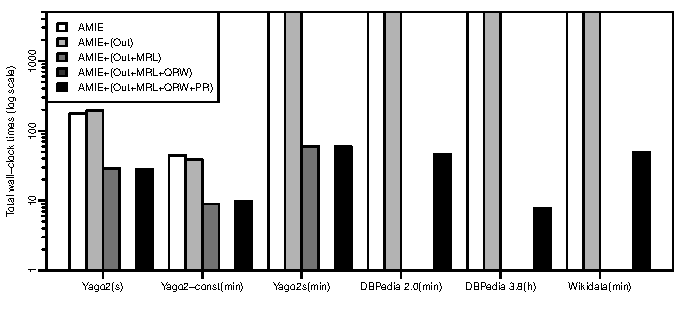
\includegraphics{figures/individual}
% \caption{Performance of individual refinement improvements}
% \label{individual}
% \end{figure*}


\paragraph{Output Comparison}
%\comment{Fabian}{Shouldn't we run AMIE also with a confidence threshold of 0.1, just to have the two comparable? Anyway, a confidence threshold of 10\% makes sense... If so, change in several places in this paper.}
%\comment{Done. Only for YAGO I rerun the experiments. For the other datasets I lie on the fact that the confidence threshold has a neglibible impact in AMIE's runtime.}
% Fabian: Meaning you reconstructed from the logs how the results would have looked, and you stayed with the old runtimes which we expect anyway to be very similar to the ones we reported because it's just a Sysout() that is avoided.
Table~\ref{outputComparison} shows a comparison of AMIE and AMIE+ in terms of output (number of rules).
For AMIE+ full we report the number of rules that were pruned by the confidence approximation.
To assess the quality of the confidence approximation, we report in addition the \emph{pruning precision}.
The pruning precision is the ratio of rules for which the confidence approximation introduced
in Section~\ref{sec:appr} overestimates the actual confidence. We
calculate this ratio by counting the number of times that the heuristics
produce a higher value than the real confidence (among the rules on which the approximation is applicable).
For example, a pruning precision of 96\% means
that in 4\% of the cases the system erroneously pruned rules with a confidence higher than 0.1.
As in the previous section, we set a threshold of 0.1 PCA Confidence for AMIE. We also interrupted the system 
if it ran more than one day. In those cases, we report the output until the point of interruption (denoted by a ``*'' in Table~\ref{outputComparison}).\footnote{Since the pruning precision was computed by comparing the output of AMIE+ to the output of AMIE, the values reported in Table~\ref{outputComparison} may have been calculated on a subset of all the rules, thus being an estimation of the actual pruning precision.} 

\begin{table}[t]
\begin{tabular}{|l|}
\hline
%\emph{y:isMarriedTo}$(x,y) \wedge$ \emph{y:livesIn}$(x,z) \Rightarrow $ \emph{y:livesIn}$(y,z)$\\
\emph{y:isCitizenOf}$(x,y) \Rightarrow$ \emph{y:livesIn}$(x,y)$\\
% \emph{hasAdvisor}$(x,y) \wedge $ \emph{graduatedFrom}$(x,z) \Rightarrow$ \emph{worksAt}$(y,z)$\\
\emph{y:wasBornIn}$(x,y) \wedge$ \emph{y:isLocatedIn}$(y,z) \Rightarrow$ \emph{y:citizenOf}$(x,z)$\\
\emph{y:hasWonPrize}$(x,G.\;W.\;Leibniz) \Rightarrow$ \emph{y:livesIn}$(x,Germany)$\\
\emph{y:hasWonPrize}$(x,Grammy) \Rightarrow$ \emph{y:musicalRole}$(x,Guitar)$\\
\emph{d:countySeat}$(x,y) \Rightarrow$ \emph{d:largestCity}$(x,y)$\\
\emph{d:jurisdiction}$(z,y) \wedge\; $\emph{d:successor}$(x,z) \Rightarrow$ \emph{d:jurisdiction}$(x,y)$\\
\emph{w:ownedBy}$(x,y) \Rightarrow$ \emph{w:subsidiary}$(y, x)$\\
\emph{w:relative}$(y,z) \wedge $\emph{w:sister}$(z, x)  \Rightarrow$ \emph{w:relative}$(x,y)$\\
\hline
\end{tabular}
\caption{Some Rules mined by AMIE on different datasets (y: YAGO, w: Wikidata, d: DBpedia).}\label{rules}
\end{table}

\begin{table}
\hspace*{-2.4ex}
\begin{tabular}{|l|}
\hline
\emph{exports}$(y,z) \wedge$ \emph{imports}$(y,z) \wedge$ \emph{livesIn}$(x,y) \Rightarrow $ \emph{citizenOf}$(x,y)$\\
%\emph{capital}$(a,f) \wedge$ \emph{hasGeoId}$(b,j) \wedge$ \emph{hasGeoId}$(f,j) \Rightarrow$ \emph{capital}$(a,b)$ \\
%\emph{currency}$(j,b) \wedge$ \emph{isLeaderOf}$(i,e) \wedge$ \emph{livesIn}$(i,a) \Rightarrow $ \emph{currency}$(a,b)$\\
\emph{diedIn}$(x,z) \wedge$ \emph{locatedIn}$(z,y) \wedge$ \emph{livesIn}$(x,z) \Rightarrow $ \emph{politician}$(x,y)$\\
%\emph{diedIn}$(f,j) \wedge$ \emph{leaderOf}$(a,f) \wedge$ \emph{locatedIn}$(j,b) \Rightarrow $ \emph{politicianOf}$(a,b)$\\
% \emph{hasOffLang}$(j,b) \wedge$ \emph{wasBornIn}$(e,a) \wedge$ \emph{wasBornIn}$(e,j) \Rightarrow $ \emph{hasOffLang}$(a,b)$\\
\hline
\end{tabular}
\caption{Examples of rules mined by AMIE on YAGO2 with $n=4$ atoms}\label{rules4atoms}
\end{table}

\begin{center}
\begin{savenotes}
\begin{table}[t]
\footnotesize
\centering
\begin{tabular}{|l| r |r r r|}
\hline
			& AMIE			& \multicolumn{3}{c|}{AMIE+(full)} 	\\ \cline{2-5}
KB			& Rules 		& Rules		&Pruned	& Prun. prec. 	   \\ \hline
  YAGO2  		& 68			& 68 		&24 	&100.00\%      	    \\ 
  YAGO2 (const)  	& 15634			& 15634		&24	&100.00\% 	    \\  
  YAGO2 (4)  		& 645			& 645		&203 	&100.00\%   	    \\ 
  YAGO2s  		& 94*			& 94	 	&78 	&100.00\%		    \\
  DBpedia 2.0 		& 24308*		& 112865	&5380 	&98.26\%      	    		\\ 
  DBpedia 3.8 		& 2470*			& 5087       	&2621 	&98.41\%	    		\\
  Wikidata  		& \textcolor{red}{746*}	& 1512		&773 	&\textcolor{red}{96.94\%}      	    \\  \hline
\end{tabular}
\caption{Output comparison of AMIE (PCA conf $\ge$ 0.1) and AMIE+ full. Starred: output after processing for 1 day. On YAGO2 (4), $maxLen=4$. On YAGO2 (const), the instantiation operator was switched on.}
\label{outputComparison}
\end{table}
\end{savenotes}
\end{center}

% Note that AMIE runs without any confidence threshold, while AMIE+ runs with confidence threshold of 0.1.
% Thus, we expect AMIE+ to output less rules than AMIE.
% However, if a system ran for more than one day, we interrupted it
% and considered the output until the point of interruption (denoted by a ``*'' in Table~\ref{outputComparison}).
%One of these cases is DBpedia 2.0, where AMIE found only 24K rules, while AMIE+(full) produces 112K rules.

As we can see, the pruning by approximation does not entail a serious decrease in the quality of the output:  
AMIE+ does not miss more than 4\% of the rules with confidence above 10\%.  
% \comment{Chris}{new:}Even when AMIE mines longer rules (maximum length 4), the confidence approximation does not appear to over-prune high-confidence rules.
At the same time, the pruning yields a speed-up by a factor of up to 3, as Table~\ref{amievsplus} shows.

\paragraph{Longer rules}\comment{chris}{new-merged with examples}
To investigate the performance of AMIE/AMIE+ with longer rules,  we ran AMIE and AMIE+ also with $maxLength=4$.  
First, notice that by constructing rules with one more atom we see almost an order of magnitude increase on the number of rules in the output (645 vs. 68, see Table~\ref{outputComparison}). 
This is indicative of how fast the search space increases for longer rules. The result is that mining on YAGO with $maxLength=4$ is 7.9x slower than on YAGO with $maxLength=3$ (see Table~\ref{amievsplus}).
% For AMIE+, we can observe a drop in the speedup offered over AMIE from 6.7x to 3x. 
In addition, the confidence approximation used in AMIE+ does not appear to over-prune high-confidence rules (100\% pruning precision) as we move to longer rules.

% \paragraph{Example rules}
Table~\ref{rules} shows some examples of highly confident rules with three and four atoms mined by AMIE on the testing datasets.
As we can observe, AMIE with its default configuration is able to mine insightful rules on large KBs. We additionally show the effect
of increasing the maximum length of rules (parameter $maxLength$ in Algorithm~\ref{rm}) to 4 atoms. Table~\ref{rules4atoms} shows
some examples.
% \comment{Luis}{TODO: Explain why rules with 4 atoms are bad}
% \comment{Chris}{why do we need to say that they are bad? before we were saying they are bad because we had no experiments for longer rules. Also the examples that you have do make sense}

\begin{table}[t]
\begin{tabular}{|l|}
\hline
%\emph{y:isMarriedTo}$(x,y) \wedge$ \emph{y:livesIn}$(x,z) \Rightarrow $ \emph{y:livesIn}$(y,z)$\\
\emph{y:isCitizenOf}$(x,y) \Rightarrow$ \emph{y:livesIn}$(x,y)$\\
% \emph{hasAdvisor}$(x,y) \wedge $ \emph{graduatedFrom}$(x,z) \Rightarrow$ \emph{worksAt}$(y,z)$\\
\emph{y:wasBornIn}$(x,y) \wedge$ \emph{y:isLocatedIn}$(y,z) \Rightarrow$ \emph{y:citizenOf}$(x,z)$\\
\emph{y:hasWonPrize}$(x,G.\;W.\;Leibniz) \Rightarrow$ \emph{y:livesIn}$(x,Germany)$\\
\emph{y:hasWonPrize}$(x,Grammy) \Rightarrow$ \emph{y:musicalRole}$(x,Guitar)$\\
\emph{d:countySeat}$(x,y) \Rightarrow$ \emph{d:largestCity}$(x,y)$\\
\emph{d:jurisdiction}$(z,y) \wedge\; $\emph{d:successor}$(x,z) \Rightarrow$ \emph{d:jurisdiction}$(x,y)$\\
\emph{w:ownedBy}$(x,y) \Rightarrow$ \emph{w:subsidiary}$(y, x)$\\
\emph{w:relative}$(y,z) \wedge $\emph{w:sister}$(z, x)  \Rightarrow$ \emph{w:relative}$(x,y)$\\
\hline
\end{tabular}
\caption{Some Rules mined by AMIE on different datasets (y: YAGO, w: Wikidata, d: DBpedia).}\label{rules}
\end{table}

\begin{table}
\hspace*{-2.4ex}
\begin{tabular}{|l|}
\hline
\emph{exports}$(y,z) \wedge$ \emph{imports}$(y,z) \wedge$ \emph{livesIn}$(x,y) \Rightarrow $ \emph{citizenOf}$(x,y)$\\
%\emph{capital}$(a,f) \wedge$ \emph{hasGeoId}$(b,j) \wedge$ \emph{hasGeoId}$(f,j) \Rightarrow$ \emph{capital}$(a,b)$ \\
%\emph{currency}$(j,b) \wedge$ \emph{isLeaderOf}$(i,e) \wedge$ \emph{livesIn}$(i,a) \Rightarrow $ \emph{currency}$(a,b)$\\
\emph{diedIn}$(x,z) \wedge$ \emph{locatedIn}$(z,y) \wedge$ \emph{livesIn}$(x,z) \Rightarrow $ \emph{politician}$(x,y)$\\
%\emph{graduatedFrom}$(x,z) \wedge$ \emph{livesIn}$(w,y) \wedge$ \emph{worksAt}$(w,z) \Rightarrow $ \emph{citizenOf}$(x,y)$\\
\emph{advisor}$(z,w) \wedge$ \emph{citizenOf}$(w,y) \wedge$ \emph{livesIn}$(z,x) \Rightarrow $ \emph{deals}$(x,y)$ \\
%\emph{diedIn}$(f,j) \wedge$ \emph{leaderOf}$(a,f) \wedge$ \emph{locatedIn}$(j,b) \Rightarrow $ \emph{politicianOf}$(a,b)$\\
% \emph{hasOffLang}$(j,b) \wedge$ \emph{wasBornIn}$(e,a) \wedge$ \emph{wasBornIn}$(e,j) \Rightarrow $ \emph{hasOffLang}$(a,b)$\\
\hline
\end{tabular}
\caption{Examples of rules mined by AMIE on YAGO2 with $n=4$ atoms}\label{rules4atoms}
\end{table}

\ignore {
\paragraph{Performance of confidence approximation w.r.t. to rule-length}
\comment{Fabian}{What is this? Will it be in the paper?}
}

% \ignore{ %% this is luis version
% Table~\ref{amievsplus} shows the runtimes of AMIE and AMIE+ with different setups on our test KBs.
% %The different setups include: default AMIE+, AMIE+ with the PCA confidence
% %bound enabled and AMIE+ with all the optimizations.
% %If a system ran for more than one day without finishing, we interrupted it and reported the Fabian: said below
% %output obtained until that point in time.
% For AMIE, we show only the runtime. Since our goal is to observe the effect of each enhancement in the runtime of AMIE+,
% we show runtimes for combinations of the improvements introduced in Sections~\ref{subsec:lossless} and~\ref{subsec:speedingConfidenceEvaluation}.
% These includes:
% \begin{enumerate}
%  \item AMIE+ in its default configuration, i.e., with the lossless enhancements: MRL + QRW + PR. We refer to this setting as \emph{Default}.
%  \item We investigate the effect of the confidence approximation by itself and call this setting \emph{AMIE+ with confidence approximation}.
%  \item We incrementally add the lossless heuristics to the last setting, leading to three additional subsettings:
%  \begin{enumerate}
%   \item AMIE+ with confidence approximation + MLR
%   \item AMIE+ with confidence approximation + MLR + QRW
%   \item AMIE+ with confidence approximation + MLR + QRW + PR or simply \emph{Full AMIE+}
%  \end{enumerate}
% \end{enumerate}
% 
% We also report the number of rules produced in each setting.
% Since the lossless enhacements do not alter the output of AMIE, we report a single rule count for settings 2 and 3.
% To assess the quality of the confidence approximation, we report in addition the \emph{pruning precision}.
% %In the default setting of AMIE+, the number of rules (and, in fact, the rules) are the same as in AMIE.
% %with and without the confidence threshold.% (confidence thresholds do not alter runtime in AMIE).
% % and when applicable the number
% % of rules with PCA confidence equal or higher than the 10\% threshold.
% % When the PCA confidence bound is enabled, we report
% % the number of rules pruned by this heuristic. We do not report the number of rules,
% % because this enhacement is lossless, that is, we obtain the same output as the default AMIE+ with a given confidence threshold.
% %When all the optimizations are enabled, we additionally show the \emph{pruning precision}.
% The pruning precision is the ratio of rules for which the confidence approximation introduced
% in Section~\ref{sec:appr} overestimates the actual confidence. We
% calculate this ratio by counting the number of times that the heuristics
% produce a higher value than the real confidence (among the rules on which the approximation is applicable).
% For example, a pruning precision of 96\% means
% that in 4\% of the cases the system erroneously pruned rules with a confidence higher than 0.1.
% If a system ran for more than one day, we interrupted it
% and considered the output until the point of interruption.
% This means that the values reported in Table~\ref{amievsplus}
% may have been calculated on a
% subset of all the rules, thus being an estimation of the actual pruning precision.
% This fact is particularly obvious
% for DBpedia 2.0, where AMIE+ found only 14K rules without confidence threshold,
% while AMIE+ with all the heuristics enabled produces 117K rules.
% 
% Table~\ref{amievsplus} shows that our enhancements have a significant impact in the runtime of AMIE.
% On YAGO2, AMIE+ already exhibits a speedup factor of 6.7 w.r.t. AMIE.
% For bigger and more complex datasets, however, even AMIE+  could not finish in one day.
% It is therefore required to enable all the optimizations to achieve reasonable runtimes.
% We can also see that the confidence upper bounds by themselves do not allow us to scale to the size of YAGO2s, DBpedia, or Freebase.
% For example, they can prune only 6 rules on YAGO2s.
% This is because they are applicable to only a very restricted set of rules, namely those of the form $r(x,z) \wedge r(y,z) \Rightarrow r_h(x,y)$ or
% $r(z,x) \wedge r(z,y) \Rightarrow r_h(x,y)$.
% Therefore, we need to enable the confidence approximations in order to scale to these KBs.
% This heuristic, however, comes with the additional cost of computing the
% join cardinalities for every pair of relations in the KB, which can be very expensive for KBs with many relations, such as DBpedia or Freebase.
% Nevertheless, it is run only once and, as the results show, it pays off.
% On KBs where normal rule mining would have required more than a day,
% AMIE+ can run in a few hours or, in the worst case, over-night.
% This speedup does not entail a serious decrease in the quality of the output:
% in the majority of datasets, AMIE+ does not miss any of the rules with confidence above 10\%.
% In the other datasets, it misses at most 4\% of them.
% }

% \begin{center}
% \begin{savenotes}
% \begin{table*}[t]
% \footnotesize
% \begin{tabular}{|l|c|c|c|c|c|c|c|c|c|c|}
% \hline
% \multirow{3}{*}{KB} 	& \multirow{3}{*}{AMIE}  	& \multicolumn{9}{c|}{AMIE+} 	\\ \cline{3-11}
% 			&  				& \multicolumn{3}{c|}{Default}		& \multicolumn{2}{c}{Upper bounds} 	& \multicolumn{4}{|c|}{Upper bounds + approx.}\\ \cline{3-11}
% 			&  				& Time & Rules & $\ge$ 10\% 		& Time & Pruned 			& Time & Rules & Pruned & Prune prec. \\ \hline
% YAGO2  			& 3.62min  			& 31.71s & 135 & 68 			& 31.21s & 3 				& 32.34s& 68 & 24 & 100\%\\
% YAGO2(const) 		& 14.09min  			& 12.17min  & 19028 & 15526 		& 12.10min & 3 				& 12.17min & 15526 & 24 & 100\% \\
% YAGO2s  		& $>$ 1 day 			& $>$ 1 day & 249 & 95  		& $>$ 1 day & 6  			& 53.2min & 95 & 78 & 100\%\\
% DBpedia 2.0  		& $>$ 1 day 			& $>$ 1 day  & 14405  & 12805 		& $>$ 1 day & 808 			& 1.77h & 117163 & 5377 & 96\%\\
% DBpedia 3.8  		& $>$ 1 day  			& $>$ 1 day   & 4215 & 2106  		& $>$ 1 day & 292 			& 8.24h & 5193 & 2621 & 97\%\\
% Freebase 		& $>$ 1 day 			& $>$ 1 day & 182  & 131 		& $>$ 1 day & 5 			& 7.51min & 169 & 37 & 100\% \\ \hline
% \end{tabular}
% \caption{Runtime and output comparison between AMIE and AMIE+ on different KBs. Times smaller than one hour are averaged over 3 runs.}
% \label{amievsplus}
% \end{table*}
% \end{savenotes}
% \end{center}

\begin{table}[t]
\begin{tabular}{p{2.3cm}|p{3cm}| p{2cm}}
\centering{Category}	& Relation 			& \% of hits	\\
\hline
Functions   		&\emph{wasBornIn} 		& 96.67\\
			&\emph{diedIn} 			& 96.42\\
			&\emph{hasCapital}		& 93.33\\
\hline
Quasi- 			&\emph{hasCurrency}		& 75\\
Functions		&\emph{hasOfficialLanguage} 	& 73.33\\
			&\emph{graduatedFrom} 		& 64.29\\
			&\emph{isCitizenOf} 		& 96.42\\
			&\emph{directed}$^{-1}$ 	& 90\\
			&\emph{hasAcademicAdvisor} 	& 88.89\\
			&\emph{created}$^{-1}$  	& 86.67\\
			&\emph{isLeaderOf} 		& 89.47\\
			&\emph{isPoliticianOf}		& 100\\
			&\emph{isAffiliatedTo}		& 89.47\\
\hline
Granularity 		&\emph{isLocatedIn}		& 50\\
Differences		&\emph{livesIn}			& 20.83\\
\hline
Implicit 		&\emph{livesIn} 		& 20.83\\
Assumptions		&&\\
\hline
Source  		&\emph{influences}$^{-1}$	& 34.78\\
Incompleteness		&\emph{imports}			& 0\\
			&\emph{exports}			& 0\\
			&\emph{actedIn}$^{-1}$		& 0\\
			&\emph{worksAt}			& 89.66\\
			&\emph{hasMusicalRole}		& 22.22\\
			&\emph{dealsWith}		& 10\\
% 			&\emph{isInterestedIn}$^{-1}$	& ?\\
% 			&\emph{isKnownFor}$^{-1}$	& ?\\
\hline
Extraction 		&\emph{participatedIn}$^{-1}$	& 48.14\\
Incompleteness		&\emph{isMarriedTo}		& 79.31\\
			&\emph{produced}$^{-1}$		& 56.67\\
			&\emph{actedIn}$^{-1}$		& 0\\
			&\emph{playsFor}		& 20\\
			&\emph{holdsPoliticalPosition}	& 26.67\\
			&\emph{hasChild}$^{-1}$		& 26.67\\
			&\emph{hasWonPrize}		& 31.03\\
			&\emph{dealsWith}		& 10\\
			&\emph{influences}$^{-1}$	& 34.78\\
			&\emph{hasMusicalRole} 		& 22.22\\
\end{tabular}
\caption{Categories of relations w.r.t. the validity of the PCA.}
\label{PCA_assumption_entities}
\end{table}




%%%%%%%%%%%%%%%%%%%%%%%%%%%%%%%%%%%%%%%%%%%%%%%

\subsection{AMIE vs. State-of-the-art Systems} \label{competitors}
% \comment{chris}{this is just a summary. Usability stuff are out. Constants on different modes are out, etc. Please see if you are happy with the result}
% Fabian: great!
In this section we compare AMIE and AMIE+ to two state-of-the-art rule mining systems 
that are publicly available:
WARMR~\cite{GoeVan02} and ALEPH~\cite{Muggleton:1996:LPD:647996.742465}. We compare the systems in terms of runtime and quality of produced rules. A more detailed description of these experiments (for AMIE), as well as a comparison of usability, can be found in~\cite{amie}.
For these experiments, we did not use any confidence threshold ($minConf=0$), and hence AMIE+ only used refinement improvements.

\subsubsection{AMIE vs. WARMR}
WARMR is a system that unifies ILP and association rule mining. Similar to APRIORI algorithms~\cite{Agrawal:1996:FDA:257938.257975}, it performs a
breadth-first search in order to find frequent patterns.
It generates Datalog queries of the form ``$?-A_1,A_2,...,A_n$'',
where $A_i$ are logical atoms. WARMR applies a closed world assumption for assessing the quality of the produced rules.

\paragraph{Runtime}
We first compare WARMR with AMIE/AMIE+ in terms of runtime only. 
For a fair comparison, we have to make sure that both systems run in the same settings. Hence, we tweaked AMIE/AMIE+ to simulate WARMR's notion of support. 
We run all systems with an absolute support threshold of 5 entities. 
We also use the standard confidence as quality metric for rules, instead of the PCA confidence.  
% \comment{Chris}{that is not true. we ran WARMR with a conf threshold=0.001}
% Since WARMR runs without confidence threshold, we set $minConf=0$ for AMIE/AMIE+. This entails that AMIE+ cannot use the confidence pruning heuristics. 

In our initial experiment, WARMR was not able to terminate on YAGO2 in a time period of 1 day. 
Therefore, we created a sample of YAGO2 containing 47K triples (see~\cite{amie} for details about the sampling method). 
Table \ref{warmrruntime} summarizes the runtime results for WARMR, AMIE, and AMIE+ on this dataset. 
We see that AMIE mines her rules in 6.02 seconds, and AMIE+ even in 3 seconds. WARMR, in contrast, took 18 hours. 

We also ran both systems in a mode that allows them to mine rules with constants. 
For AMIE, this means enabling the instantiation operator $\mathcal{O}_I$ (see Section~\ref{subsubsec:refinement}).
AMIE and AMIE+ completed the task in less than 2 minutes. WARMR, in contrast, did not terminate in 3 days.
Therefore, we ran it only for the relations \textit{diedIn}, \textit{livesIn}, \textit{wasBornIn}, for which it took 48h. 
% To make AMIE+ comparable, we run it without confidence threshold, therefore the reported runtime for AMIE+ uses only the enhancements for the refinement phase. % Fabian: I moved that to above.
% Thus, AMIE and AMIE+ are better suited for mining rules on large KBs than WARMR.
To understand this drastic difference, one has to take into account that WARMR is an ILP algorithm written in a logic programming environment, 
which makes the evaluation of all candidate queries inefficient.

\begin{table}
\begin{tabular}{l|rr rr|}
Constants 	& WARMR 		& AMIE 		& AMIE+\\
\hline
 no 		& 18h 			& 6.02s 	& 2.59s \\
 yes 		& (48h) 	 	& 1.43min  	& 1.45min\\
\end{tabular}
\caption{Runtimes on YAGO2 sample}
\label{warmrruntime}
\end{table}


\paragraph{Results} After filtering out non-connected rules, WARMR mined 41 closed rules. 
AMIE and AMIE+, in contrast, mined 75 closed rules, which included the ones mined by WARMR.
We checked back with the WARMR team and learned that for a given set of atoms $B_1, ... B_n$, 
WARMR will mine only one rule,
picking one of the atoms as head atom (e.g., $B_1 \wedge ... \wedge B_{n-1} \Rightarrow B_n$).
AMIE, in contrast, will mine one rule for each possible choice of head atom (as long as the thresholds are met).
In other words, AMIE with the standard support and confidence measures simulates WARMR, but mines more rules.
Furthermore, it runs orders of magnitude faster. 
Especially for large datasets for which the user would have needed to use complicated sampling schemes in order to use WARMR,
AMIE can be a very attractive alternative.
Even for smaller datasets with rules with constants, AMIE can provide results while WARMR cannot.
Moreover, AMIE does not make a closed world assumption as WARMR does. 
%uses the PCA confidence to measure the quality of rules comes with metrics that go beyond the standard confidence and the standard support.
In Section~\ref{experimentspca} we show that the PCA confidence defined by AMIE
is more suitable than the standard confidence to identify predictive rules in a web-extracted KB designed under
an open world assumption.

\subsubsection{AMIE vs. ALEPH}

ALEPH is an ILP system that implements a variety of scoring functions for measuring a rule's quality. For our experiments we used the 
\emph{Positives-only} evaluation function~\cite{Muggleton:1996:LPD:647996.742465,usir1753}, 
which is the most interesting for our setting, since it does not require the existence of explicit negative examples.
It takes random facts as negative evidence, instead:
\[ Score := log(P)-log\frac{R+1}{Rsize+2}-\frac{L}{P} \]
Here, $P$ is the number of known true facts covered (KBtrue, or A resp., in Figure~\ref{fig:prediction}), $R$ is the number of random examples covered, 
$Rsize$ is the total number of randoms, and $L$ is the number of atoms in the rule. 
The intuition behind the formula is that a good rule should cover many positive examples, and few or no randomly generated examples. This ensures
that the rule is not overly general. Furthermore, the rule should use as few atoms as possible.%, and thus achieve a high compression.



\paragraph{Runtime}
We ran AMIE, AMIE+ and ALEPH on YAGO2. For ALEPH, we used the positive-only evaluation function with $Rsize=50$ 
and we considered only clauses that were able to explain at least 2 positive examples,
so that we will not get grounded facts as rules in the output.
For a fair comparison, we also instructed AMIE and AMIE+ to run with a support threshold of 2 facts.
% We did not use any confidence threshold ($minConf=0$), and hence AMIE+ could not use the confidence pruning heuristics.

Table \ref{alephrun0} shows the results. AMIE terminated in 4.41 minutes and found rules for all relations. AMIE+ was slightly faster.
ALEPH runs for one head relation at a time. For some relations (e.g.\emph{isPoliticianOf}),
it terminated in a few seconds.
For others, however, we had to abort the system after 1 day without results (Table \ref{alephrun1}).
For each relation, ALEPH treats one positive example at a time. Some examples need little processing time, others block the system for hours.
We could not figure out a way to choose examples in such a way that ALEPH runs faster.
Hence, we used the sample of YAGO2 that we created for WARMR.
Again, runtimes varied widely between relations (Table \ref{alephrun2}).
Some relations ran in a few seconds, others did not terminate in a day.
% The runtimes with constants are similarly heterogeneous, with at least 7 relations not terminating in 1 day \comment{Luis}{I propose
% to remove this sentence as it may raise the reviewer's curiosity about the runtimes of ALEPH with constants. }. 
% \comment{Fabian}{If we have those times, add them to the discussion. If we don't, remove the last sentence.}
% \comment{Luis}{Chris, do we have those times?}
% \comment{Chris}{they do not appear in the original amie paper. I am taking it out}

\begin{table}
\begin{tabular}{l|ccc}
KB & ALEPH & AMIE & AMIE+\\
\hline
YAGO2 full & 4.96s to $>$ 1 day & 4.41min & 3.76min\\
YAGO2 Sample & 0.05s to $>$ 1 day & 5.65s & 2.90s \\
\end{tabular}
\caption{Runtimes ALEPH vs. AMIE/AMIE+}
\label{alephrun0}
\end{table}
\begin{table}[t]
 \begin{tabular}{l|r}
Relations & Runtime\\
\hline
isPoliticianOf, hasCapital, hasCurrency & $<$ 5min\\
dealsWith, hasOfficialLanguage, imports & $<$ 5min\\
isInterested, hasMusicalRole & $<$19min\\
hasAcademicAdvisor, hasChild& $>$ 1 day\\
isMarriedTo, livesIn, worksAt, isLocatedIn& $>$ 1 day\\ %[-0.4cm]
\end{tabular}
\caption{Runtimes of ALEPH on YAGO2}
\label{alephrun1}
\end{table}
\begin{table}[t]
\begin{tabular}{l|r}
Relations & Runtime\\
\hline
diedIn, directed, hasAcademicAdvisor & $<$ 2min\\
graduatedFrom, isPoliticianOf, playsFor & $<$ 2min\\
wasBornIn, worksAt, isLeaderOf &  $<$ 2min\\
exports, livesIn, isCitizenOf & $<$ 1.4h\\
actedIn, produced, hasChild, isMarriedTo & $>$ 1 day\\ %[-0.4cm]
\end{tabular}
\caption{Runtimes of ALEPH on YAGO2 sample}
\label{alephrun2}
\end{table}

\paragraph{Results}
We compared the output of ALEPH with the positives-only evaluation function to the output of AMIE/AMIE+ using the PCA
confidence on the sample of YAGO2 used for the runtime experiments.
Since ALEPH requires more than one day for some relations, so we used only rules for which the head
relation runs in less than one day.
ALEPH mined 56 rules, while AMIE mined 302 rules.
We ordered the rules by decreasing score (ALEPH) and decreasing PCA confidence (AMIE).
Table \ref{alephres} shows the number of predictions and their total precision.
We show the aggregated values at the points where both approaches have produced around 3K, 5K, and 8K predictions.
AMIE's PCA confidence succeeds in sorting the rules roughly by descending precision, so that the initial rules have an extraordinary precision 
compared to ALEPH's.
AMIE needs more rules to produce the same number of predictions as ALEPH (but she also mines more).

\begin{table}
\begin{tabular}{l|rrr}
	    & Top $n$ & Predictions & Precision \\
 \hline
 Positives-only & 7 & 2997 & 27\% \\
 PCA Confidence & 12 & 2629 & 62\% \\
 \hline
 Positives-only & 9 & 5031 & 26\% \\
 PCA Confidence & 22 & 4512& 46\% \\
 \hline
 Positives-only & 17 & 8457 & 30\% \\
 PCA Confidence & 23 & 13927  & 43\% \\
\end{tabular}
\caption{PCA confidence vs. positives-only score: aggregated precision of rules mined on YAGO2 sample.}
\label{alephres}
\end{table}

We suspect that ALEPH's positives-only evaluation function manages to filter out overly general rules only to some extent.
The reason is that this measure ``guesses'' negative examples at random, whereas rules usually create false predictions in a non-random way.
Even if a rule produces many false predictions, the intersection of these false predictions and the random counterexamples may be very small.
Consider for example the rule $bornIn(x,y) \Rightarrow diedIn(x,y)$, which produces false predictions for example for persons who have moved
to a different place during their life.
By creating negative examples just by considering random person-location pairs,
we might not produce any case for which the rule will give a false prediction,
simply because such a negative example will have a relatively small probability to be generated.
% ALEPH will mine, e.g., \emph{livesIn}$(A,C),$\emph{isLocatedIn}$(C,B) \Rightarrow$ \emph{isPoliticianOf}$(A,B)$.
% The problem is that ALEPH generates counterexamples by randomly using valid constants for variables $A$ and $B$.
% Hence, the probability of creating a random example in which $B$ is the place of residence of the specific person $A$ is very low.\\

\paragraph{Summary}
Our experimental results show that AMIE (and in particular AMIE+) can be up to 3 orders of magnitude faster
than other state-of-the-art systems, namely WARMR~\cite{GoeVan02} and ALEPH~\cite{Muggleton:1996:LPD:647996.742465}.
The PCA confidence was shown to rank productive and correct rules higher than other confidence metrics.


\subsection{Evaluation of the PCA} \label{experimentspca}
The Partial Completeness Assumption (PCA) says that if, for a given subject $s$ and a given relation $r$, the KB knows one object $o$ with $r(s,o)$, then the KB knows \emph{all} objects $o'$ with $r(s,o')$ (Sec.~\ref{sec:pca}). The original AMIE paper used the PCA but it did not evaluate whether this assumption is true or not \cite{amie}.
Since the PCA is one of the basic ingredients of AMIE's mining model,
we wanted to know to what extent this assumption holds in a real-world KB.

\paragraph{Setup} We looked into each of the 31 relations between entities in YAGO2.
For each relation $r$, we randomly sampled 30 subjects.
For each subject $x$, we checked whether the KB knows all $y$ with $r(x,y)$. If the relation is more inverse functional than functional
($ifun(r) > fun(r)$, see Section~\ref{subsec:functions}), we considered $r^{-1}$ instead.

As a ground truth, we took the Wikipedia page of $x$ and what we could find on the Web by a search engine.
It is obvious that such an evaluation cannot be done strictly quantitatively.
For example, a person might have worked for a company, but this fact might appear nowhere on Wikipedia -- or even on the Web.
Or a musician might play 10 instruments at different levels of proficiency, but Wikipedia mentions only the 4 main instruments.
Even a search on the Web might not tell us that there are more than 4 instruments.
Therefore, we resorted to a qualitative analysis.
We analyzed each of the relations manually, and grouped the relations into categories.
Some relations fall into multiple categories.
Table~\ref{PCA_assumption_entities} shows, for each relation, the percentage of subjects in our sample for which the PCA holds.

\paragraph{Functions and Quasi-Functions} By definition, the PCA holds for functions. Our manual analysis, however, did not result in 100\% precision for functional relations in Table~\ref{PCA_assumption_entities}.
This is because our analysis also counts the cases where the KB contains bugs. If, for instance, YAGO knows the wrong place of death of a person, then there exists another value outside YAGO that is the right value. However the PCA would reject it. Hence, we count this case as a miss.

The PCA extends well to relations that are strictly speaking not functions, but that have a high functionality.
These are relations that usually have one object per subject, even though there could be several objects.
For example, a person can graduate from several universities, but most people graduate from a single university. We call these relations \emph{quasi-functions}.
The PCA worked very well also on these, and predicted completeness correctly for $73\%-100\%$
of the subjects under investigation. Since the PCA takes into account the direction of the functionality, the PCA also holds for quasi inverse-functional relations such as \emph{directed}.

\paragraph{Granularity Differences} Some relations, such as \emph{locatedIn} and \emph{livesIn}, hold between an entity and a geographical region.
In that case, the region can be given at the granularity of a city, a region, a country, or a continent.
Naturally, if YAGO contains one of these, the others are possible options. Hence, PCA fails and we found rather low precision values.
However, these cases could be addressed if one restricts the range of the relation (say, to cities).
With such a restriction, the relations become functions or quasi-functions, which lifts them into the category where the PCA works well.
% We plan to investigate this possibility in future work.
As we will see in Section~\ref{prediction}, the use of types can significantly improve the performance of AMIE.

\paragraph{Implicit Assumptions} Some statements can be inferred from the Wikipedia page even if the page does not mention them. % For instance, %\emph{livesIn} is incomplete ``in-purpose'' in the sense
People usually do not state information that can easily be inferred by what they have stated before
(following Grice's Maxim of quantity and manner~\cite{grice}). %\footnote{\url{http://www.usingenglish.com/articles/grices-conversational-maxims.html}}).
For example, if someone graduated from a university, people usually do not feel obliged to mention that this person used to live in the country
 in which the university is located,
because this can easily be inferred by the reader. Only less obvious residences will be explicitly mentioned. Therefore, the PCA does not always hold.
Note that rules such as $graduatedFrom(x,y)\Rightarrow livesIn(x,y)$ can only be mined if Grice's maxims are occasionally violated by the authors of the articles.
If the authors always follow the maxims, then such rules cannot be mined, because there are not even positive examples for which the rule holds (lack of support).
In the case of YAGO, the only relation that we found in this category is \emph{livesIn}.


\paragraph{Source Incompleteness} For many relations, the source itself (Wikipedia) is incomplete.
Usually, these relations have, for each subject, some objects that are undisputed.
For example, it is undisputed that Albert Einstein is interested in physics. However, these relations also have objects that are less important, disputed, or unknown.
For example, Albert Einstein might also be interested in music (he played the violin), but maybe also in pancakes.
These less prominent objects are a lot less likely to appear in Wikipedia, or indeed on any Web page.
Even if they do, we can never be sure whether there is not still something else that Einstein was interested in.
For these relations, the knowledge sources are often incomplete by nature.
For example, not every single product that a country imports and exports is explicitly mentioned.
Whether or not this poses a problem depends on the application.
If ground truth is defined as what is universally true, then source incompleteness is a problem.
If ground truth is the source of the KB (i.e., Wikipedia in this case), then source incompleteness is not an issue.



\paragraph{Extraction Incompleteness} For a large number of relations, the Wikipedia page contains more objects for a given subject than the KB.
These are cases where the extraction process was incomplete.
In the case of YAGO, this is due to a strong focus on accuracy,
which causes the extraction to discard any extracted fact that cannot be type checked or linked to an entity.
This class of relations is the most sensitive category for the PCA.
The success of the PCA will depend on how many relations and to what extent they are affected by incomplete extractions.

\paragraph{Discussion} In summary, our analysis shows that it depends on the nature of the relation and on its type signature whether the PCA holds or not.
 There is a large number of relations for which the PCA is reasonable.
These are not just functions and inverse functions, but also relations that exhibit a similar behavior.

For many other cases, the PCA does not hold. In these cases, AMIE will falsely assume that a rule is making incorrect predictions -- although, in reality,
the predictions might be correct.
Thus, when the PCA does not hold, AMIE will err on the side of caution.

At the same time, the PCA is not as restrictive as the closed world assumption (CWA):
the PCA admits that there can be facts that are true, but not known to the KB.
For example, if a person has a birth date, then both the CWA and PCA would not admit another birth date. However, if a person does not have a birth date, then the PCA will admit that there can be a birth date, while the CWA will assume that there cannot be a birth date. Thus, the PCA is more permissive than the CWA.
This encourages us to use the PCA for the definition of our confidence. In the following, we will show that this definition of confidence produces
 more predictive and more accurate rules than the standard confidence, which is based on the CWA.

%\subsubsection{Standard Confidence vs. PCA Confidence }
\subsection{Predicting Facts}
\label{prediction}

\paragraph{Prediction} One of the applications of the mined rules could be to predict new facts. 
Based on what the KB knows, one aims to predict what else might be the case in the real world. 
This is a difficult endeavor: It amounts to guessing the places of residence for people, their birth place, or even their death place. 
Naturally, we may not assume a high precision in the prediction of the future. We may only expect educated guesses.

To evaluate the precision of these guesses, we proceeded as follows: 
We ran our system with the default setting on the YAGO2 dataset. 
For each rule, we evaluated whether the predictions that go beyond YAGO2 were true. 
We did this by either checking whether the prediction appears in a newer version of the KB (YAGO2s), 
or by manually checking them in Wikipedia. If we could find the predicted fact in neither, we evaluated it as false.

\paragraph{Standard vs PCA confidence} Our first goal is to see whether the PCA confidence or the standard confidence perform better in this task. 
Since both AMIE and AMIE+ can work with both confidence metrics, and since their output is the same, we report here our results from \cite{amie} with AMIE. 
We ran AMIE, and sorted the resulting rules first by descending PCA confidence, and then by descending standard confidence. 
We looked at the top ranked rules in each case, and evaluated the precision of the predictions. 
The bottom curves of Figure \ref{finalshow} plot the aggregated predictions versus the aggregated precision for the standard and the PCA confidence.
The $n$-th dot from the left represents the total number of unique predictions and the total precision of these predictions,
aggregated over the first $n$ rules.
As we see, ranking the rules by standard confidence is a very conservative approach:
It identifies rules with reasonable precision, but these do not produce many predictions.
Going down in the list of ranked rules, the rules produce more predictions -- but at lower precision.
The top 30 rules produce 113K predictions at an aggregated precision of 34\%.
In contrast, if we rank the rules by PCA confidence, we quickly get large numbers of predictions. The top 10 rules already produce 135K predictions -- at a precision of 45\%.
The top 30 rules produce 3 times more predictions than the top 30 rules by standard confidence -- at comparable precision.
This is because the PCA confidence is less conservative than the standard confidence. 
We thus conclude that the PCA confidence is better suited for making predictions than the standard confidence. 
We show in \cite{amie} that the PCA confidence also correlates better with the actual precision of a rule.

\begin{figure}
%\hspace*{-5ex}
%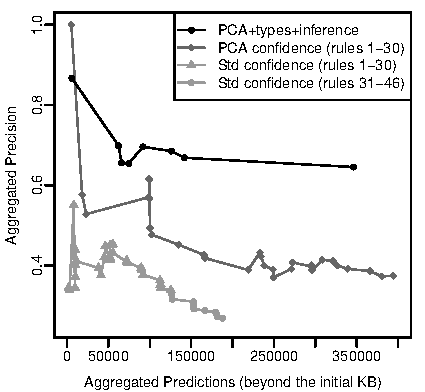
\includegraphics{figures/std_vs_pca}\ %\\[-0.5cm]
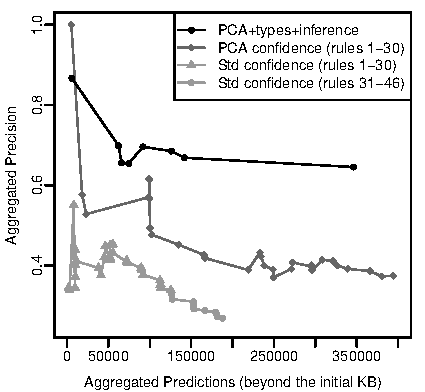
\includegraphics[width=0.5\textwidth]{figures/std_vs_pca}
\caption{Std. confidence vs. PCA confidence}
\label{finalshow}
\end{figure}

\paragraph{Using Type Information}
%The naive prediction approach presented in~\cite{amie} was designed as a proof of concept  to show the suitability of the PCA confidence as precision metric for rules mined on a Web-extracted KB. 
The previous experiment showed us the precision of individual rules for prediction. 
%A precision of 35\% is not high enough to make actual predictions about the death place, future spouse, or future residence of a person. 
To make more accurate predictions, we have to combine these rules with more signals. 
We proceed as follows. In Section~\ref{PCA_assumption_entities} we discussed the granularity
differences in relations. For instance, the relation $livesIn$ is used to express a person's city or country of residence. 
This implies that, for example, the rule 
$livesIn(x, y) \Rightarrow isCitizenOf(x, y)$ can predict that some people are citizens of cities. Such spurious predictions decrease the precision
of the inference process. Therefore, we configured AMIE+ to mine \emph{typed rules}. These have the form:
\[
 \vec{B} \wedge \textit{rdf:type}(x, D) \wedge \textit{rdf:type}(y, R) \Rightarrow r(x, y)
\]

\noindent where $D$ and $R$ correspond to the domain and range of the head relation $r$ in YAGO3\footnote{We used YAGO3 because the type signatures in older versions were too general for some relations.}.
% With a PCA confidence threshold of 0.1, AMIE+ found 57 typed rules on YAGO2.
%This constraint suffices to solve the granularity differences discussed in Section~\ref{PCA_assumption_entities} as, for example, YAGO defines the relation $livesIn$ between people and cities.

\paragraph{Joint Prediction} Our second observation is that the same prediction can be fired from multiple rules. If we consider rules as signals of evidence,  
then facts predicted by more rules should get a higher confidence score. 
In YAGO2, 9\% of the predictions are fired by more than one rule (with a PCA confidence threshold of 0.1).  
To take this into account, we changed the way predictions are ranked. In the original experimental setup, if 
multiple rules $R_1, \dots R_k$ made a prediction $p$, the prediction was only counted the first time it was fired. 
Since the rules were ranked by decreasing PCA confidence, 
this was equivalent to rank predictions according to their highest PCA confidence: 
\[
 score(p) := max\{conf_{pca}(R_1), \dots, conf_{pca}(R_k) \}
\]
We propose an alternative score instead:
\begin{equation}\label{predictions-score}
 score^*(p) := 1 - \prod_{i = 1}^{k}{(1 -conf_{pca}(R_i)})
\end{equation}
Equation~\ref{predictions-score} aggregates the PCA confidence of the rules so that the predictions concluded by multiple rules
are ranked higher. It also confers a probabilistic interpretation to the PCA confidence. The score of a prediction
is the probability that at least one of the rules in $R_1, \dots R_k$ concludes $p$. This is computed as 1 minus the probability
that none of the rules concludes $p$. The probability of a rule not concluding $p$ is defined as 1 minus the PCA confidence of the rule.
The probability that none of the rules concludes $p$ is the product of the individual probabilities.
Although this scoring-scheme is very simplistic (assumes independence of rules, uses confidences as probabilities), it can still serve as  
a naive baseline for probabilistic inference methods. In practice, more involved methods can be used (\cite{markovlogic,urdf}) with better results.


% Equation~\ref{predictions-score} assumes that rules are independent of each other. While this assumption may not always be true,
% it still serves as a naive baseline for probabilistic inference methods.




\paragraph{Results} The upper curve in Figure~\ref{finalshow} shows the precision of the predictions made with both heuristics. 
We proceeded as in the previous experiment, that is,
we first used the rules to fire predictions, and then we ranked these predictions by descending score and computed their cumulative precision. 
Unlike in the original experimental setup, the n-th point from the left in the new curve corresponds to the cumulative precision
of the predictions up to the n-th bucket. We bucketized the predictions by score using a bucket size of 0.1, i.e., the first point
corresponds to the predictions with score between 1 and 0.9, the next one accounts for the predictions with score between 0.9 and 0.8 and so on.

As we can observe, our heuristics have a significant effect on the precision of the predictions. 
The precision is much higher at each level of recall, compared to the original experiment. 
We can make 100,000 predictions at a precision of 70\%. At 400K predictions, we still achieve a precision of 60\%. 
While these predictions should not be added directly to a KB, they could be sent to human evaluators to check their correctness.
It is much easier for a person to check fact candidates for their correctness than to invent them from scratch.
In addition, this experimental setup could serve as a naive baseline for more sophisticated inference approaches.

%such a simple approach guarantees than more than a half of the predictions
% could be  it could still become a useful way
% a human evaluator
% could checked them The predicted candidates could be checked by a human before adding them to the KB.
% It is much easier for a person to check fact candidates for their correctness than to invent them from scratch.
% We will investigate this avenue of research in future work.

% While, such experimental
%  Nevertheless, this experimental setup could
%  serve as a naive baseline for more sophisticated inference approaches. In particular, the
% predictions in KBs is
% has been widely studied in the literature, however the experimental setup disregards two important characteristics of the data and the rule mining process.
% In

% As we can see, the PCA confidence ranks predictive rules higher and is therefore more suitable for data prediction than the standard confidence.
% Nevertheless, rule mining with the PCA confidence achieves a cumulative precision in the range of 35\%-45\%.
%
% This precision is certainly not high enough to make actual predictions about the death place, future spouse, or future residence of a person. However, such rules can still be useful for downstream applications. For example, if several rules predict the same fact, then this fact is more likely to be true. Hence, we could use our predictions to construct a probabilistic KB that weights each fact by the number of rules that predicted it. Facts with high cumulated confidence could be good candidates to populate KBs.
% The predicted candidates could be checked by a human before adding them to the KB. It is much easier for a person to check fact candidates for their correctness than to invent them from scratch. We will investigate this avenue of research in future work.
% The predicted statements could also be used in ontology watermarking schemes such as in~\cite{DBLP:conf/www/SuchanekG12}. These schemes add plausible but wrong statements to the KB in order to mark it. Rule mining can deliver such statements.
%
% We also note that our rules are insightful. Table \ref{rules} shows some of the rules that we mined.
% Being able to mine reasonable rules on semantic KBs of this size is an achievement beyond the current state of the art.

% \ignore{
% \begin{table}
% \hspace*{-3.4ex}
% \begin{tabular}{|l|}
% \hline
% \emph{isMarriedTo}$(x,y)\ \wedge$ \emph{livesIn}$(x,z) \Rightarrow $ \emph{livesIn}$(y,z)$\\
% \emph{isCitizenOf}$(x,y) \Rightarrow$ \emph{livesIn}$(x,y)$\\
% \emph{hasAdvisor}$(x,y)\ \wedge $ \emph{graduatedFrom}$(x,z) \Rightarrow$ \emph{worksAt}$(y,z)$\\
% \emph{wasBornIn}$(x,y)\ \wedge$ \emph{isLocatedIn}$(y,z) \Rightarrow$ \emph{isCitizenOf}$(x,z)$\\
% \emph{hasWonPrize}$(x,G.\;W.\;Leibniz) \Rightarrow$ \emph{livesIn}$(x,Germany)$\\
% \emph{hasWonPrize}$(x,Grammy) \Rightarrow$ \emph{hasMusicalRole}$(x,Guitar)$\\
% \hline
% \end{tabular}
% \caption{Several rules mined by AMIE}
% \label{rules}
% \end{table}
% }
%\ignore{
% \paragraph{Precision of Mined Rules}
% In general, we can also use the confidence measures to estimate the actual precision of a rule.
% When mining rules, we are naturally interested in using an evaluation measure that correlates well with the real precision of a rule.
% To compare standard and PCA confidence, we ranked the mined rules by their actual precision.
% Table~\ref{cor-new} shows the average absolute error of the standard and PCA confidence weighted by the number of predictions produced by the rules based on the following formula:
%
% \[
%  Error = \frac{\sum \limits_{r \in Output}{|Precision(r)-Conf(r)|\#Facts(r)}}{\sum \limits_{r \in Output}{\#Facts(r)}}
% \]
% %
% We observe that, on average, the PCA confidence estimates the precision of the rules better than the standard confidence.
% Thus, reasoning approaches can use the PCA confidence as a weight for the rule.
%
% Note also that the PCA confidence is much closer to the actual precision value than the standard confidence for the top 20 rules.
% Since the error of PCA confidence is much smaller than the error of the standard confidence for the best performing rules (in terms of the actual precision),
% our results also imply that such rules have higher chances of being discovered during the mining process if we use the PCA confidence as quality evaluation metric.
%
%
% \begin{table}
% \small
% \begin{tabular}{l|ccc}
% 		& Top 20 rules 	&Top 30 rules	&All rules	\\
% \hline
% Confidence 	& 0.67		&0.49		&0.29 \\
% PCA Confidence 	& 0.28		&0.25		&0.28 \\
% \end{tabular}
% \caption{Average absolute prediction error (over new facts)}
% \label{cor-new}
% \end{table}
% }
% \begin{table}
% \begin{tabular}{l|rrr}
% 	    & Top $n$ & Predictions & Precision \\
%  \hline
%  Positives-only & 7 & 2997 & 27\% \\
%  PCA Confidence & 12 & 2629 & 62\% \\
%  \hline
%  Positives-only & 9 & 5031 & 26\% \\
%  PCA Confidence & 22 & 4512& 46\% \\
%  \hline
%  Positives-only & 17 & 8457 & 30\% \\
%  PCA Confidence & 23 & 13927  & 43\% \\
% \end{tabular}
% \caption{PCA confidence vs. positives-only score: aggregated precision of rules mined on YAGO2 sample.}
% \label{alephres}
% \end{table}

% \ignore{
% \subsubsection{PCA Confidence vs. Positives-Only Score}
% We compared the output of ALEPH with the positives-only evaluation function to the output of AMIE using the PCA
% confidence on the sample of YAGO2 used for the runtime experiments.
% Recall that ALEPH requires more than one day for some relations, so we used only rules for which the head
% relation runs in less than one day.
% ALEPH mined 56 rules, while AMIE mined 306 rules.
% We order the rules by decreasing score (ALEPH) and decreasing PCA confidence (AMIE).
% Table \ref{alephres} shows the number of predictions and their total precision.
% We show the aggregated values at the points where both approaches have produced around 3K, 5K, and 8K predictions.
% AMIE's PCA confidence succeeds in sorting the rules roughly by descending precision, so that the initial rules have an extraordinary precision compared to ALEPH's.
% AMIE needs more rules to produce the same number of predictions as ALEPH (but she also mines more).
% We suspect that ALEPH's positives-only evaluation function manages to filter out overly general rules only to some extent.
% ALEPH will mine, e.g., \emph{livesIn}$(A,C),$\emph{isLocatedIn}$(C,B) \Rightarrow$ \emph{isPoliticianOf}$(A,B)$.
% The problem is that ALEPH generates counterexamples by randomly using valid constants for variables $A$ and $B$.
% Hence, the probability of creating a random example in which $B$ is the place of residence of the specific person $A$ is very low.\\
% }







%%%%%%%%%%%%%%%%%%%%%%%%%%%%%%%%%%%%%%%%%%%%%%%%%%%%%%%%%%%%%%%%%%%%%%%%%%%%%%
%% previous version after this point


% \subsection{Overview}%\ \\[-0.7cm]
% \label{eval}
%
% \paragraph{Experiments}
% Before developing on the main experiments, we describe our datasets and
% experimental setup and provide a justification
% for the selection of rules up to 3 atoms. Then we describe our three main groups of experiments, where we
% (i) conduct an empirical evaluation of the PCA assumption on YAGO; (ii)
% compare AMIE and AMIE+ to two popular, state-of-the-art systems that are publicly available,
% WARMR~\cite{DehToi99,DehToi00} and ALEPH$^{\ref{foot:aleph}}$, and (iii) compare in detail
% the performance improvements of AMIE+ w.r.t AMIE.


% \paragraph{Settings} By default, AMIE uses a head coverage threhold of $\theta=1\%$ and
% ranks the resulting rules by decreasing PCA confidence. There is no need to deviate from this default configuration when a user runs AMIE.
% There are no parameters to tune. Moreover, AMIE+ inherits this default behavior and extends it by enabling the lossless optimizations (see Section~\ref{prunebound})
% in order to guarantee a faster execution without affecting the output.
% All experiments with AMIE/AMIE+ on all datasets are run in these settings, unless otherwise mentioned.
%
% \paragraph{Comparison with other systems} For some experiments, we want to compare AMIE's runtime and rule quality with other systems.
% To have an equal basis, we make AMIE
% simulate the metrics of the competitor systems.
% AMIE can threshold on support, head coverage, confidence, and PCA confidence, and she can rank by any of these.
% By default the system counts support on the two head variables, however it can also count on one of them. This variable can be
% always on the same position (e.g., always the subject) or can vary depending on the head relation. In that case, AMIE counts on the functional
% variable of the relation (see Section~\ref{subsec:functions} about functions).
% AMIE can also output non-closed rules. Since this is just a choice of what to output, it does not influence runtime.
% All experiments are run on a server with 48GB of RAM and 8 CPUs (Intel Xeon at 2.4GHz).
% We always mine rules without constants (i.e., without the instantiation operator), unless otherwise mentioned.
%
%
% \www{
% \paragraph{Knowledge Bases} We run our experiments on different KBs.
% In all cases, we removed the \emph{rdf:type} relationship, because it inflates the size of the KBs.
% We are aware that the \emph{rdf:type} relationship can be very helpful for rule mining.
% However, currently no approach (including ours) makes specific use of it.
% We plan to make use of it in future work. Furthermore, we removed all facts with literals (numbers and strings) from the KBs.
% Literal values (such as geographical coordinates) are shared by only very few entities, which makes them less interesting for rule mining.
% }
% Table~\ref{kbs} shows a summary of the KBs used for our experiments.
%
% \begin{savenotes}
% \ffigure{Table}{kbs}{Knowledge Bases used to test AMIE/AMIE+}{
% \footnotesize
% \begin{tabular}{l|c|c|c}
% KB & Facts & Subjects & Relations\\
% \hline
% YAGO2  & 948K & 470K & 32\\
% YAGO2s & 4.12M  & 1.65M & 37\\
% DBpedia 2.0 & 6.70M & 1.38M & 1595\footnote{This corresponds to the relations with more than 100 facts.} \\
% DBpedia 3.8 & 11.02M & 2.20M & 650 \\
% Freebase (people) & 8.92M & 2.07M & 51
% \end{tabular}
% }
% \end{savenotes}
%
% \subsection{Optimal length of rules}
% AMIE can in principle mine closed Horn rules with an arbitrary number of atoms, however all our experiments
% mine rules up to three atoms. This was decided from the observation than
% rules with more than three atoms are much more numerous and noisy. To support this assertion, we ran
% AMIE+ on YAGO2 with maximum rule length $n=4$ in order to investigate the quality of longer rules.
% Some of them are listed in Table~\ref{rules4atoms}. Let us look at one of the examples: \\
%
% {\small \raggedleft \emph{capital}$(a,f) \wedge$ \emph{hasGeoId}$(b,j) \wedge$ \emph{hasGeoId}$(f,j) \Rightarrow$ \emph{capital}$(a,b)$} \\
%
% It is easy to see that $f$ and $b$ bind always to the same values since the relations $hasCapital$ and $hasGeonamesId$ are
% highly functional. This makes the rule not interesting at all. Such kind of patterns arise because AMIE's
% language bias allows multiple atoms with the same relation. We could prune these type of rules by enforcing
% the constraint $f \neq b$ in the database, however inequality constraints
% come at expense of lower performance. We name these kind of rule patterns,
% \emph{subgraph redundant rules}%~\comment{Luis}{SOS: I cannot think of a better name}
% , since they contain groups of atoms (subgraphs) that bind to the same values
% and are thus redundant. We
% therefore tweaked AMIE to filter such cases. Another way to avoid these kind of rules, is to allow relations to appear
% at most once in each rule. We report running time and the number of rules mined by AMIE+
% with exactly 4 atoms with different settings in Table~\ref{yago4atoms}.
% The removal of subgraph redundant rules does not affect runtime because the rules are pruned after they are mined.
% %\comment{Chris}{in the rule or in the rule's body? Am I still able to get: you live where your spouse lives?}
% In contrast, avoiding repeated relations in atoms has a big impact in runtime and the size of the output.\\
%
% {\small
% \ffigure{Table}{rules4atoms}{Examples of high-confidence rules mined by AMIE with $n=4$ atoms}{
% \hspace*{-2.4ex}
% \begin{tabular}{|l|}
% \hline
% \emph{exports}$(b,h) \wedge$ \emph{imports}$(b,h) \wedge$ \emph{livesIn}$(a,b) \Rightarrow $ \emph{citizenOf}$(a,b)$\\
% \emph{capital}$(a,f) \wedge$ \emph{hasGeoId}$(b,j) \wedge$ \emph{hasGeoId}$(f,j) \Rightarrow$ \emph{capital}$(a,b)$ \\
% \emph{currency}$(j,b) \wedge$ \emph{isLeaderOf}$(i,e) \wedge$ \emph{livesIn}$(i,a) \Rightarrow $ \emph{currency}$(a,b)$\\
% \emph{diedIn}$(f,j) \wedge$ \emph{leaderOf}$(a,f) \wedge$ \emph{locatedIn}$(j,b) \Rightarrow $ \emph{politicianOf}$(a,b)$\\
% % \emph{hasOffLang}$(j,b) \wedge$ \emph{wasBornIn}$(e,a) \wedge$ \emph{wasBornIn}$(e,j) \Rightarrow $ \emph{hasOffLang}$(a,b)$\\
% \hline
% \end{tabular}
% }
% }
% \ffigure{Table}{yago4atoms}{AMIE on YAGO2 with maximum rule length $n=4$}{
% \small
% \begin{tabular}{l|c|c|}
% Setting & Runtime & Rules \\
% \hline
% Default & \multirow{2}{*}{5.71min} &  2144  \\
% No redundant subgraphs &  & 1231\\
% No repeated relations & 1.49min &  132 \\
% \end{tabular}
% }
%
% \paragraph{Discussion} Table~\ref{rules4atoms} shows some confident rules with 4 atoms. Our observations on the whole set of rules
% suggest that increasing the rule size does not provide a practical benefit: runtime increases as well as the number of uninteresting rules.
% Longer rules are also more complex to understand. The notion of length and complexity for hypotheses, is one of the key points of the
% Minimum Description Length principle, where among two hypotheses explaining the data comparably well, the simpler (shorter) is preferred.
% Furthermore, ILP approaches such as~\cite{Muggleton95inverseentailment} take into account this principle, giving preference to shorter rules.

% \begin{center}
% \begin{savenotes}
% \begin{table*}[t]
% \captionsetup{justification=centering, labelfont=bf}
% \setcounter{table}{\value{figureCounter}}
% \stepcounter{figureCounter}
% \footnotesize
% \begin{tabular}{|l|c|c|c|c|c|c|c|c|c|c|}
% \hline
% \multirow{3}{*}{KB} & \multirow{3}{*}{AMIE}  & \multicolumn{9}{c|}{AMIE+} \\ \cline{3-11}
%   &  & \multicolumn{3}{c}{Lossless}  & \multicolumn{2}{|c}{Upper bounds} & \multicolumn{4}{|c|}{Upper bounds + approx.}\\ \cline{3-11}
%   &  & Time & Rules & $\ge$ 10\% & Time & Pruned & Time & Rules & Pruned & Prune prec. \\ \hline
% YAGO2  & 3.62min  & 31.71s & 135 & 68 & 31.21s & 3 & 32.34s& 68 & 24 & 100\%\\
% YAGO2(const) & 14.09min  & 12.17min  & 19028 & 15526 & 12.10min & 3 & 12.17min & 15526 & 24 & 100\% \\
% YAGO2s  & $>$ 1 day & $>$ 1 day & 249 & 95  & $>$ 1 day & 6  & 53.2min & 95 & 78 & 100\%\\
% DBpedia 2.0  & $>$ 1 day & $>$ 1 day  & 14405  & 12805 & $>$ 1 day & 808 & 1.77h & 117163 & 5377 & 96\%\\
% DBpedia 3.8  & $>$ 1 day  & $>$ 1 day   & 4215 & 2106  & $>$ 1 day & 292 & 8.24h & 5193 & 2621 & 97\%\\
% Freebase & $>$ 1 day & $>$ 1 day & 182  & 131 & $>$ 1 day & 5 & 7.51min & 169 & 37 & 100\% \\ \hline
% \end{tabular}
% \centering\caption{\textbf{Runtime and output comparison between AMIE and AMIE+ on different KBs. Times smaller than one hour are averaged across 3 runs.}}
% \label{amievsplus}
% \end{table*}
% \end{savenotes}
% \end{center}

% \subsection{The PCA for Rule Mining}
%
% The PCA is the central assumption of AMIE's mining model. We conducted two rounds experiments to assess its feasibility.
% In the first round, we investigate how often the PCA holds in a web-extracted KB like YAGO, whereas in the second round
% we compare the performance of the PCA confidence against the standard confidence for data prediction under incompleteness.
%
% \subsubsection{PCA in Knowledge Bases}
% The PCA is the assumption that if a KB knows some values $r$-values for an entity $x$, then the entity does not have
% any other $r$-values. As discussed in Section~\ref{pcaEvaluation}, the PCA holds
% for functions and quasi-functions, whereas for other relations may be too optimistic
% about the completeness of the KB. Since the PCA is crucial in AMIE's mining model, we conducted an experiment
% to quantify how often it is wrong, that is, we estimated the ratio of cases when the KB did not know all
% the $r$-values of an entity. For this purpose, we constructed a sample of YAGO2s in
% in such a way that each relation occurs with 30 different random subjects. Then we
% verified for each pair entity-relation, whether the KB was actually complete.
% For instance, if YAGO knows about the two daughters of Barack Obama (i.e., Natasha and Malia) and there is no evidence about any other
% children in Wikipedia, the
% PCA is correct and this is counted as hit. On the contrary, if Wikipedia shows evidence about another child not present in YAGO,
% this counts as a miss. We show the percentage of hits per relation in Table~\ref{PCA_assumption}.

% \ffigure{Table}{PCA_assumption_entities}{Categories of relations w.r.t. the PCA}{
% \begin{tabular}{p{2cm}|p{5.4cm}}
% \centering{Category}		  & Relations 	\\
% \hline
% Functions   & \emph{wasBornIn}, \emph{diedIn}, \emph{hasCapital}\\%,  \comment{Chris}{have we evaluated those guys?} \comment{Luis: }{These relations do not exist in YAGO2, only in YAGO2s} \emph{happenedIn}, \emph{hasPredecessor}, \emph{owns}$^{-1}$ \\
% \hline
% Quasi-Functions & \emph{hasCurrency}, \emph{hasOfficialLanguage}, \emph{graduatedFrom}, \emph{isCitizenOf}, \emph{directed}$^{-1}$, \emph{hasAcademicAdvisor}, \emph{created}$^{-1}$,  \emph{isLeaderOf}, \emph{isPoliticianOf}\\%, \comment{Chris}{have we evaluated those guys?} \emph{wroteMusicFor}$^{-1}$\\
% \hline
% Granularity Differences& 	\emph{isLocatedIn},  \emph{livesIn}\\%,\comment{Chris}{have we evaluated those guys?} \emph{happenedIn}\\
% \hline
% Implicit Assumptions&\emph{livesIn} \\
% \hline
% Source Incompleteness & \emph{influences}$^{-1}$, \emph{imports}, \emph{exports}, \emph{actedIn}$^{-1}$, \emph{worksAt}, \emph{hasMusicalRole}, \emph{dealsWith}, \emph{isInterestedIn}$^{-1}$, \emph{isKnownFor}$^{-1}$\\
% \hline
% Extraction Incompleteness& \emph{participatedIn}$^{-1}$, \emph{isMarriedTo}, \emph{produced}$^{-1}$,  \emph{actedIn}$^{-1}$, \emph{playsFor}, \emph{holdsPoliticalPosition}, \emph{hasChild}$^{-1}$,  \emph{hasWonPrize}, \emph{dealsWith},\emph{influences}$^{-1}$, \emph{hasMusicalRole}\\
% \end{tabular}
% }

% \ffigure{Table}{PCA_assumption}{Ratio of cases the PCA is wrong for relations}{
% \begin{tabular}{p{2cm}|l|c}
% \textbf{Category} & \textbf{Relation} & \% of hits 	\\
% \hline
% % \multirow{3}{*}{Functions}  & $created^{-1}$	&77.78	\\
% %   & $diedIn$		&96.43	\\
% %   & $hasCapital$		&93.33	\\
% \multirow{9}{*}{\parbox{2cm}{{\small Quasi Functions}}}  &  $hasCurrency$&75	\\
% & $hasOfficialLanguage$	&73.33	\\
% & $graduatedFrom$	&64.29	\\
% & $isCitizenOf$		&96.42	\\
% & $directed^{-1}$	&90 	\\
% & $hasAcademicAdvisor$	&88.89	\\
% & $created^{-1}$	&86.67	\\
% & $isLeaderOf$		&89.47	\\
% & $isPoliticianOf$	&100	\\
% & $isAffiliatedTo$	&89.47 \\ \hline
% {\small Granularity differences} &   $isLocatedIn$	&50	\\ \hline
% {\small Implicit assumptions} & $livesIn$		&20.83	\\ \hline
% \multirow{5}{*}{\parbox{2cm}{{\footnotesize Source incompleteness}}} & $influences$		&34.78	\\
%    & $imports^{-1}$	&0	\\
%    & $actedIn^{-1}$	&0	\\
%    & $worksAt$		&89.66	\\
%    & $dealsWith$		&10\\ \hline
% \multirow{9}{*}{\parbox{2cm}{{\small Extraction incompleteness}}} &  $participatedIn^{-1}$	&48.14	\\
% & $isMarriedTo^{-1}$	&79.31	\\
% & $produced^{-1}$	&56.67	\\
% & $playsFor$		&20	\\
% & $produced^{-1}$	&56.67	\\
% & $holdsPoliticalPosition$	&26.67\\
% & $hasWonPrize$		&31.03\\
% & $hasChild^{-1}$	&26.67	\\
% & $hasWonPrize$		&31.03\\
%
% \end{tabular}
% }
% \comment{Luis}{We may group them according to the classification proposed in Section 4.4}
% \comment{Chris}{I agree. Perhaps we should just move this discussion in 4.4 (i.e. report the numbers there) or move 4.4 here.}
% We make use of the FUN-property of KBs (see Section~\ref{subsec:functions}), so that relations are always more functional than inverse functional in the
% evaluation. If this is not the case for a relation $r$, we use its inverse $r^{-1}$. This guarantees the evaluation of completeness goes always in the same direction: given
% a subject and a relation, we verify the completeness of the object values. We omitted functions such as $wasBornIn$
% in Table~\ref{PCA_assumption} since the PCA holds by definition for those relations. Some relations may fall within more than one category
% according to Section~\ref{pcaEvaluation} but we assign them to a single category in Table~\ref{PCA_assumption}
%
% \paragraph{Discussion}
% %Note that despite these problems, % Fabian: There is no problem, PCA is great! :-)
% We see that the PCA performs well in general in the rule mining scenario.
% This is true in particular if we compare it to the alternative, the Closed World Assumption (CWA).
% The CWA would reject all statements that are not in the KB.
% This includes the statements that the PCA assumes to be false. Thus, there are cases in which both assumptions err.
% For example, if the KB contains only one parent of a child, then both assumptions would (erroneously) reject an additional parent.
% One way to mitigate this, would be to learn an ``expected cardinality'' of a relation, and to reject as false everything
% that deviates too much from this cardinality.
% % \comment{Luis}{We should also consider the
% % standard deviation or maybe the whole probability distribution of the cardinality.}
% % This, however, would require coordination across rules if the number of objects in the KB falls more than 1 object short of the expected cardinality
% % -- something that we defer to future work.
% % \comment{Chris}{I didn't get it} \comment{Luis}{This is also not clear to me.}
% In all other cases, the PCA is more accurate than the CWA:
% The CWA will not admit a birthplace for a person that does not have a birthplace in the KB. The PCA will.
% Likewise, the CWA will not admit parents for a child that does not have parents in the KB, while the PCA does.
% This shows that the PCA is more careful when producing negative examples. This helps AMIE mine more productive rules,
% as we show in the next section.

% \subsection{Standard confidence vs. PCA confidence}
%
% In this section, we compare the standard confidence measure to the PCA confidence measure as ranking metric for rules.
% The comparison is based on the number and precision of predictions of the most confident rules according to each metric.
% % Our discussion includes a comparison of their predictions as well as the results of our empirical
% % evaluation of the PCA assumption.
%
% \subsubsection{Number of Predictions}
%
% We ran AMIE with the vanilla setting on the YAGO2 dataset. It contains nearly 500K entities and 948K facts.
% We sorted the rules first by descending PCA confidence, and then by descending standard confidence, and looked at the top rules.
% For each rule, we evaluated the predictions beyond YAGO2 %\comment{Katja}{Shouldn't it be ``beyond YAGO''?}\comment{Chris}{We train in Yago2, we test in yago2s. This is ok.}
% as described in Section \ref{eval}.
% Figure \ref{finalshow} plots the aggregated predictions versus the aggregated precision.
% The $n$-th dot from the left represents the total number of predictions and the total precision of these predictions, aggregated over the first $n$ rules.
% As we see, ranking the rules by standard confidence is a very conservative approach:
% It identifies rules with reasonable precision, but these do not produce many predictions.
% Going down in the list of ranked rules, the rules produce more predictions -- but at lower precision. The top 30 rules produce 113K predictions at an aggregated precision of 34\%.
% In contrast, if we rank the rules by PCA confidence, we quickly get large numbers of predictions. The top 10 rules already produce 135K predictions -- at a precision of 45\%.
% The top 30 rules produce 3 times more predictions than the top 30 rules by standard confidence -- at comparable precision.
% This is because the PCA confidence is less conservative than the standard confidence.
%
%
% \www{
% \ffigure{Figure}{finalshow}{Std. Confidence vs. PCA Confidence}{
% \hspace*{-5ex}
% 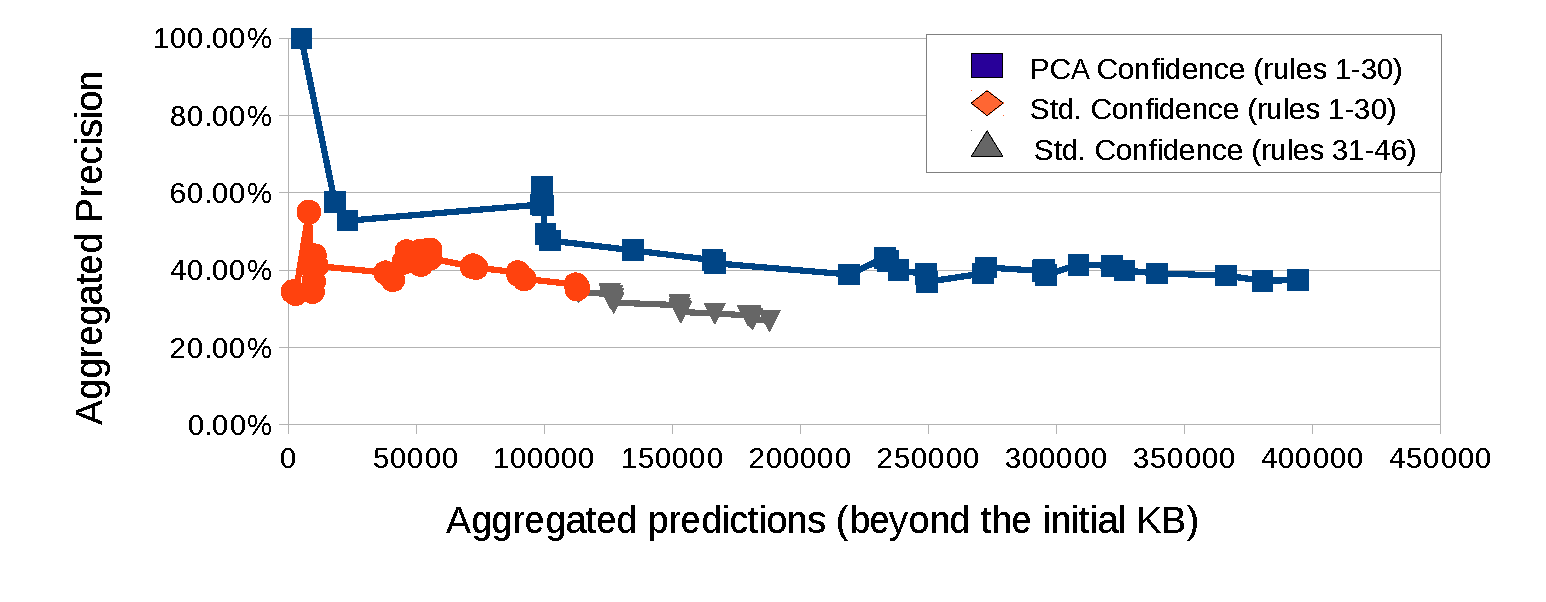
\includegraphics[scale=0.38]{figures/pca_vs_std_confidence.pdf}\ \\[-0.5cm]
% \comment{Katja}{Does anyone have a good idea how to increase readability of the chart? The green triangles are hard to distinguish from the red diamonds.}
% }
% }

% \paragraph{Discussion} The goal of the above experiment was to compare the quality of the rules that PCA confidence and standard confidence can mine.
% As we can see, the PCA confidence ranks predictive rules higher and is therefore more suitable for data prediction than the standard confidence.
% Nevertheless, rule mining with the PCA confidence achieves a cumulative precision in the range of 35\%-45\%. This happens because
% each rule by itself is imperfect.
% It is important to remark, however, that in a real life scenario where the quality of the derived facts matters,
% one should not just produce facts by deduction, like we did in this experiment. Rules should instead be used as building blocks
% for different applications. For example, while most of the predictions may not be true, they are still
% plausible statements that could be used in ontology watermarking schemes as in~\cite{conf/semweb/SuchanekGA11}.
% We can construct probabilistic KBs based on the predictions produced by the rules. For instance, multiple rules predicting the same fact,
% can have an additive effect on the confidence we have about that fact. Facts with high confidence are good candidates to populate KBs.
% If one wants to add those facts to the KB through a system that makes use
% of human agents, then reducing the number of potentially false predictions (i.e., facts with little statistical evidence)
% is a great advantage.


% \www{
% We also note that our rules are insightful. Table \ref{rules} shows some of the rules we mined. Being able to mine reasonable rules on semantic KBs of this size is an achievement beyond the current state of the art.\\
% }
%
% \www{
% \ffigure{Table}{rules}{Some Rules mined by AMIE}{
% \hspace*{-2.4ex}
% \begin{tabular}{|l|}
% \hline
% \emph{isMarriedTo}$(x,y) \wedge$ \emph{livesIn}$(x,z) \Rightarrow $ \emph{livesIn}$(y,z)$\\
% \emph{isCitizenOf}$(x,y) \Rightarrow$ \emph{livesIn}$(x,y)$\\
% \emph{hasAdvisor}$(x,y) \wedge $ \emph{graduatedFrom}$(x,z) \Rightarrow$ \emph{worksAt}$(y,z)$\\
% \emph{wasBornIn}$(x,y) \wedge$ \emph{isLocatedIn}$(y,z) \Rightarrow$ \emph{isCitizenOf}$(x,z)$\\
% \emph{hasWonPrize}$(x,G.\;W.\;Leibniz) \Rightarrow$ \emph{livesIn}$(x,Germany)$\\
% \emph{hasWonPrize}$(x,Grammy) \Rightarrow$ \emph{hasMusicalRole}$(x,Guitar)$\\
% \hline
% \end{tabular}
% }
% }


% \subsubsection{Precision of the Predictions}
% In general, we can also use the confidence measures to estimate the actual precision of a rule.
% When mining rules, we are naturally interested in using an evaluation measure that correlates well with the real precision of a rule.
% To compare standard and PCA confidence, we ranked the mined rules by their actual precision.
% Table~\ref{cor-new} shows the average absolute error of the standard and PCA confidence weighted by the number of predictions produced by the rules based on the following formula:
%
% \[
%  Error = \frac{\sum \limits_{r \in Output}{|Precision(r)-Conf(r)|\#Facts(r)}}{\sum \limits_{r \in Output}{\#Facts(r)}}
% \]
% %
% We observe that, on average, the PCA confidence estimates the precision of the rules better than the standard confidence.
% Thus, reasoning approaches can use the PCA confidence as a weight for the rule.
%
% Note also that PCA confidence is much closer to the actual precision value than the standard confidence for the top 20 rules. %\comment{Katja}{Maybe add the actual precision values to the table?}
% Since the error of PCA confidence is much smaller than the error of the standard confidence for the best performing rules (in terms of the actual precision),
% our results also imply that such rules have higher chance to be discovered during the mining process, if we use the PCA confidence as quality evaluation metric.
%
% \comment{Katja}{We will have to explain why the numbers here are so different from the WWW paper}
% \comment{Chris}{The evaluation is different (I think). We could point this out in the cover letter. My concern is more why we are converging in our errors with std conf.
% It means we screw up consistently whereas std confidence behaves very well at some point in the end.}
%
% \ffigure{Table}{cor-new}{Average Absolute Prediction Error \\(over new facts)}{
% \small
% \begin{tabular}{l|ccc}
% 		& Top 20 rules 	&Top 30 rules	&All rules	\\
% \hline
% Confidence 	& 0.67		&0.49		&0.29 \\
% PCA Confidence 	& 0.28		&0.25		&0.28 \\
% \end{tabular}
% }

% \subsection{AMIE vs. AMIE+}
% In this section we discuss the runtime improvements of AMIE+, which enable us to run on very large datasets.
% AMIE+ extends the original system AMIE with two types of enhacements:
%
% \paragraph{Lossless optimizations} They include Maximum Rule Length and Query Rewriting and Caching.
% These improvements do not alter the completeness of AMIE, i.e., they do not prune the output, but still allow for faster mining. AMIE+ enables them by default.
% \comment{Chris}{Why is confidence upper bound grouped as lossy optimization here? In the AMIE+ section it is under the lossless category. After all it
% is not an approximation.}
%
% \paragraph{Lossy optimizations} They include pruning by confidence upper bounds and by confidence approximations.
% These improvements might alter the output of AMIE since they prune rules that are expected to be low confident and very expensive to mine.
% Unlike the lossless heuristics, they require a minimum confidence threshold. For the type of rules discussed in Section~\ref{upperBound},
% the confidence upper bounds let us know precisely if the
% confidence of a rule will be below the confidence threshold, before calculating the actual confidence score. Our confidence
% approximations, on the other hand,
% provide a rough estimation of the confidence score which can be both an overestimation or underestimation of
% the actual confidence score. Underestimation affects the completeness of AMIE+,
% since some rules with high confidence score may be pruned. In any case, calculating the confidence upper bounds or estimating the confidence
% is much cheaper than computing the actuak confidence. All the experiments involving the lossy heuristics use a confidence
% threshold of 10\% PCA confidence.
%
%
% Table~\ref{amievsplus} shows the running times of AMIE and AMIE+ on our test KBs. For the latter, we display
% the running time with different configurations: default AMIE+ (i.e., only lossless heuristics enabled), AMIE+ with confidence
% bounds and AMIE+ with all the optimizations. If the system runs more than one day without finishing, we interrupted it and reported the
% output obtained until that point in time.
% For AMIE we show the runtime reported in~\cite{amie}. For the default configuration of AMIE+,
% we show the running time, the total number of rules
% and the number of rules with PCA confidence equal or higher than 10\%. Note that for
% all KBs except YAGO2, AMIE+ (only lossless heuristics enabled) could not finish in one day.
% The situation is not much different when we only enable the PCA confidence bounds with threshold 10\%. For this setup,
% we report the running time
% and the number of rules pruned by this heuristic. When all the optimizations are enabled, we report runtime, number of rules output, number of rules
% pruned by the heuristics and the pruning precision. The pruning precision is the ratio of rules for which the confidence approximation introduced
% in Sec.~\ref{subsec:pruningbyapprox} overestimates the actual confidence. We
% calculate this ratio by counting the number of times the heuristic produces a higher value than the real confidence in the set of rules output
% by AMIE+ (where the approximation is applicable) with the default setup within one day of running.
% \comment{Chris}{Why count the times that we overestimated confidence? in this cases we will not prune. We should count the cases that we underestimated confidence
% and pruned nice rules.}
% This means the value reported on Table~\ref{amievsplus}
% was calculated on a
% subset of all the rules and is actually an approximation of the pruning precision. This fact is particularly obvious
% for DBpedia 2.0 where AMIE+ found
% only 12K rules over the 10\% threshold, whereas enabling all the heuristics produces 117K rules
% \comment{Chris}{Are these rules in total or rules above 10\%? If it is the first let's compare it with the rules in total of AMIE+}.
%
%
% Table~\ref{amievsplus} shows that our enhancements have a significant impact on the systems runtime. On YAGO2 and even without the more aggresive lossy enhacements,
% AMIE+ exhibits a
% speedup of 6.7x with respect to AMIE. For bigger and more complex datasets, it is required to enable all the optimizations to achieve reasonable running times.
% We can also see that the confidence upper bounds by themselves do not allow us to scale to the size of YAGO2s, DBpedia or Freebase. For example they can prune only
% 6 rules on YAGO2s. This occurs because they are applicable to a very restricted set of rules; those of the form $r(x,z) \wedge r(y,z) \Rightarrow r_h(x,y)$ or
% $r(z,x) \wedge r(z,y) \Rightarrow r_h(x,y)$. Therefore, to scale we need to enable the confidence approximations.
% This heuristic, however, comes with the additional cost of computing the
% join cardinalities for every pair of relations in the KB, which can be very expensive for KBs with many relations such as DBpedia or Freebase.
% Nevertheless, it is run only once and, as the results show, it pays off.
% \comment{Chris}{Do we have perhaps the time needed for preprocessing for these datasets?
% We could report total time and preprocessing time and then this argument can also be seen in the table.}



% \subsection{AMIE vs. WARMR and ALEPH}
% \noindent In this section, we compare AMIE to WARMR and ALEPH. For each system, we conduct 3 experiments: We first compare the usability of the competitor system to AMIE.
% Then, we compare their runtimes with AMIE and AMIE+. Last, we compare their outputs.
%
% \subsubsection{AMIE vs. WARMR}
%
% \www{
% \paragraph{Usability} WARMR is a system that unifies ILP and association rule mining. Similar to APRIORI algorithms~\cite{Agrawal:1996:FDA:257938.257975}, it performs a
% breadth-first search in order to find frequent patterns.
% WARMR generates Datalog queries of the form ``$?-A_1,A_2,...,A_n$'',
% where $A_i$ are logical atoms.
% }
%
% \www{
% To discover frequent patterns (as in association rule mining), we need to have a notion of frequency. Given that WARMR considers queries as patterns and that queries can have variables,
% it is not immediately obvious what the frequency of a given query is. Therefore, the user needs to specify
% %define what is actually
% the predicate that is being counted by the system (the \textit{key predicate}).
% Since the key predicate determines what is counted, it is necessary that it is contained in all queries.
% For this reason, WARMR starts with having nothing but the key predicate in the body of the rule and then constructs more rules by adding more predicates.
% In the usual scenario of market basket analysis, the system counts customer transactions.
% In a scenario in which the database is a KB, one solution is to count entities.
% Therefore, we add a predicate \emph{entity}$(x)$, which we fill with all entities of the KB}. On the contrary, AMIE does not require such a trick.
%
% For WARMR, the user needs to provide specific information (called type declarations) about which predicates can be added to a query, which of their variables can be fresh (output mode),
% which should have already appeared in another atom (input mode)
% and which can be both (input/output mode). In other words, the user needs to define the language bias in terms of type and mode declarations.
% In order to stay as close as possible to AMIE's language bias, each relation should have at least one variable with input/output mode, so that fresh variables can be introduced in the rules.
% For functional or inverse functional relations, we declared subjects (objects) with an input mode and objects (subjects) with an input/output mode.
% %\comment{Luis}{Just to be sure 100\% sure, WARMR always starts with the key predicate, right? If yes, we should state it. }
% For relations that are not clearly functional or inverse functional (e.g. \emph{actedIn}, \emph{hasChild}) we declared both variables with input/output mode.
% According to the type declaration we used, the rules output by WARMR are neither necessarily closed nor connected.
% In general, WARMR does not differentiate between intermediate constructed rules (e.g. connected, but not closed) and final rules (e.g. closed).
% This means that the user needs to filter out the useful rules for his application from all the intermediate constructed rules.
% % Therefore, we had to filter out from the output non-interesting rules for our scenario rules . % Fabian: "non-interesting" sounds very subjective
% For the comparison with AMIE, we filtered out non-closed and non-connected rules.
%
% \www{
% WARMR is also able to mine rules with constants. The user can define which predicates and arguments should be instantiated with constants (we call this mode MODE1).
% WARMR then checks all the constants appearing in the facts of that specific predicate and argument and afterwards uses them in the queries.
% MODE1 naturally entails an increase of the branching factor in the search space and an explosion in the number of candidates that need to be evaluated.
% Alternatively, WARMR allows the user to set a maximum number of constants to be used for each predicate and argument (MODE2).
% Unfortunately, though, it does not provide a way for the user to influence the selection of these constants.
% In other words, there is no guarantee that the constants that WARMR will use are the most promising ones} in terms of support.
%
% \www{
% Thus, we conclude that the broader mission and the broader applicability of WARMR entails that much more configuration, acquaintance, and expert knowledge is needed to make it mine Horn rules on semantic KBs.
% }
%
% \www{
% \paragraph{Runtime}
% YAGO2\cite{yago2} contains around 940K facts about 470K entities.
% WARMR was not able to terminate on this data in a time period of 1 day. Therefore, we created a sample of YAGO2.
% Randomly selecting a number of facts from the initial dataset could break the interesting links between the entities.
% Therefore, we randomly selected 10,000 seed entities and included their 3-hop neighborhood.
% This yielded 14K entities and 47K facts.
% This sample contains all available information in a radius of 3 hops around the seed entities, but much less information about the entities at the periphery of the subgraph.
% Therefore, we restricted the values for the key predicate
% to the seed entities only.
% }
%
% Since the sample is much smaller than the original KB, we lowered the support threshold to 5 entities.
% In order to make AMIE and WARMR comparable, we tweaked AMIE so that she will also count seed entities while calculating the standard confidence.
% We ran AMIE with the same parameters on the sample. AMIE mined her rules in 7.91s seconds on average across 3 runs.
% WARMR, in contrast, took 18 hours.
% We also ran both systems allowing them to mine rules with constants. AMIE completed the task in 1.68 minutes on average. WARMR in MODE1 for all relations did not terminate in 3 days.
% Therefore, we ran it also only for the relations \textit{diedIn}, \textit{livesIn}, \textit{wasBornIn}, for which it took 48h. We also ran WARMR in MODE2.
% To have reasonable runtimes, we allowed WARMR to find constants only for one predicate (\emph{diedIn}). We also restricted it to find only 20 constants. WARMR ran 19 hours.
% Table \ref{warmrruntime} summarizes the runtime results for WARMR, AMIE and AMIE+. We conclude that AMIE is better suited for large KBs than WARMR.
% This is because WARMR is an ILP algorithm written in a logic programming environment, which makes the evaluation of all candidate queries inefficient.\\
%
% \ffigure{Table}{warmrruntime}{Runtimes on YAGO2 sample}{
% \footnotesize
% \begin{tabular}{l|rr rr|}
% Constants & WARMR & AMIE & AMIE+\\
% \hline
%  no & 18h & 7.91s & 5.24s \\
%  yes & (48h) / (19.3h) & 1.68min  & 1.06min\\
% \end{tabular}
% }
%
% \www{
% \paragraph{Results} After filtering out non-connected rules, WARMR mined 41 closed rules. AMIE+, in contrast, mined 207 closed rules, which included the ones mined by WARMR.
% We checked back with the WARMR team and learned that for a given set of atoms $B_1, ... B_n$, WARMR will mine only one rule, picking one of the atoms as head atom (e.g., $B_1 \wedge ... \wedge B_{n-1} \Rightarrow B_n$).
% AMIE, in contrast, will mine one rule for each possible choice of head atom (as long as the thresholds are met). In other words, AMIE with the standard support and confidence measures simulates WARMR, but mines more rules.
% Furthermore, it runs orders of magnitude faster. Especially for large datasets for which the user would have needed to use complicated sampling schemes in order to use WARMR, AMIE can be a very attractive alternative.
% Even for smaller datasets with rules with constants, AMIE can provide results while WARMR cannot. Moreover, AMIE comes with metrics that go beyond the standard confidence and the standard support.
% We will show later that these improve the quality of the results.
% }
%
% \www{
% \subsubsection{AMIE vs. ALEPH}
%
% \paragraph{Usability} ALEPH can be run with different commands that influence the search strategy. We chose the \emph{induce} command, which runs fastest.
% For running ALEPH, the user has to specify the target predicate for learning (the head predicate of the rules).
% In the following, we ran ALEPH successively with all predicates of the KB as targets.
% In addition, the user has to specify a series of type and mode declarations (similar to WARMR), which will be used as a language bias in order to restrict the search space.
% In addition, the user needs to provide ALEPH with files containing the background knowledge and positive examples for the target predicate.
% In contrast, AMIE requires no such input. It will run on a KB without any prespecified choices of predicates.\\
% }
%
%
% \ffigure{Table}{alephrun0}{Runtimes ALEPH vs. AMIE/AMIE+}{
% \footnotesize
% \begin{tabular}{l|ccc}
% KB & ALEPH & AMIE & AMIE+\\
% \hline
% YAGO2 full & 4.96s to $>$ 1 day & 3.62min & 1.62min\\
% YAGO2 Sample & 0.05s to $>$ 1 day & 7.91s & 2.27s \\
% \end{tabular}
% }
%
% \www{
% \ffigure{Table}{alephrun1}{Runtimes of ALEPH on YAGO2}{ % no constants
% %\begin{flushleft}
% \begin{tabular}{l|r}
% Relations & Runtime\\
% \hline
% isPoliticianOf, hasCapital, hasCurrency & $<$ 5min\\
% dealsWith, hasOfficialLanguage, imports & $<$ 5min\\
% isInterested, hasMusicalRole & $<$19min\\
% hasAcademicAdvisor, hasChild& $>$ 1 day\\
% isMarriedTo, livesIn, worksAt, isLocatedIn& $>$ 1 day\\ %[-0.4cm]
% \end{tabular}
% %\end{flushleft}
% } %\ \\[-1cm]
%
% \ffigure{Table}{alephrun2}{Runtimes of ALEPH on YAGO2 sample}{
% %\begin{flushleft}
% \begin{tabular}{l|r}
% Relations & Runtime\\
% \hline
% diedIn, directed, hasAcademicAdvisor & $<$ 2min\\
% graduatedFrom, isPoliticianOf, playsFor & $<$ 2min\\
% wasBornIn, worksAt, isLeaderOf &  $<$ 2min\\
% exports, livesIn, isCitizenOf & $<$ 1.4h\\
% actedIn, produced, hasChild, isMarriedTo & $>$ 1 day\\ %[-0.4cm]
% \end{tabular}
% %\end{flushleft}
% }%\ \\[-1cm]
% }
%
% \www{
% \paragraph{Runtime}
% We ran AMIE and ALEPH on YAGO2 \cite{yago2}. For ALEPH, we used the positive-only evaluation function with $Rsize=50$ and we considered only clauses that were able to explain at least 2 positive examples,
% so that we will not get grounded facts as rules in the output.
% For a fair comparison, we also instructed AMIE to run with a support threshold of 2 facts.
% AMIE terminated in 3.62 minutes, and found rules for all relations. ALEPH ran for one head relation at a time. For some relations (e.g.\emph{isPoliticianOf}),
% it terminated in a few seconds.
% For others, however, we had to abort the system after 1 day without results (Tables \ref{alephrun0} and \ref{alephrun1}).
% For each relation, ALEPH treats one positive example at a time. Some examples need little processing time, others block the system for hours.
% We could not figure out a way to choose examples in such a way that ALEPH runs faster.
% Hence, we used the sample of YAGO2 that we created for WARMR.
% %, which contains around 47k facts for a variety of target predicates.
% Again, runtimes varied widely between relations (Table \ref{alephrun2}).
% Some relations ran in a few seconds, others did not terminate in a day.
% The runtimes with constants are similarly heterogeneous, with at least 7 relations not terminating in 1 day.
% }
%
% \paragraph{Results}
% We compared the output of ALEPH on the head relations for which it terminated to the output of AMIE on these head relations, on the sample dataset.
% ALEPH mined 56 rules, while AMIE mined 306 rules.
% We order the rules by decreasing score (ALEPH) and decreasing PCA confidence (AMIE).
% Table \ref{alephres} shows the number of predictions, and their total precision as described in Section \ref{eval}.
% We show the aggregated values at the points where both approaches have produced around 3K, 5K, and 8K predictions.
% AMIE's PCA confidence succeeds in sorting the rules roughly by descending precision, so that the initial rules have an extraordinary precision compared to ALEPH's.
% AMIE needs more rules to produce the same number of predictions as ALEPH (but she also mines more).
% We suspect that ALEPH's positives-only evaluation function manages to filter out overly general rules only to some extent.
% ALEPH will mine, e.g., \emph{livesIn}$(A,C),$\emph{isLocatedIn}$(C,B) \Rightarrow$ \emph{isPoliticianOf}$(A,B)$.
% The problem is that ALEPH generates counterexamples by randomly using valid constants for variables $A$ and $B$.
% This means that the probability of creating a random example in which $B$ is the place of residence of the specific person $A$ is very low.\\
%
% \ffigure{Table}{alephres}{Top Rules of ALEPH vs. AMIE on YAGO2 sample}{
% \begin{tabular}{l|rrr}
%  System & Top $n$ & Predictions & Precision \\
%  \hline
%  ALEPH & 7 & 2997 & 27\% \\
%  AMIE & 12 & 2629 & 62\% \\
%  \hline
%  ALEPH & 9 & 5031 & 26\% \\
%  AMIE & 22 & 4512& 46\% \\
%  \hline
%  ALEPH & 17 & 8457 & 30\% \\
%  AMIE & 23 & 13927  & 43\% \\
% \end{tabular}
% }
%
%
%
%
%
%
% \subsection{AMIE for Data Prediction}
% As a simple proof of concept, we ran AMIE on older versions of YAGO (YAGO2)\cite{yago2} and DBpedia (2.0)\cite{dbpedia}
% and used to the rules to make predictions which we verified in newer versions of the KBs, YAGO2s and DBpedia 3.8.
% We report in Table~\ref{dbp} the number of predicted facts that are in the newer version of the KB but not in the old one (hits).
% A fact can be predicted by multiple rules, so we report the count with and without duplicates.
% The results show that logical rules can be used to generate
% a large number of plausible facts. Moreover, evidence from multiple rules can increase
% the confidence we have on a fact. This suggests a potential for the development of more sophisticated models
% to estimate the accuracy of our precisions and identify facts that are more likely true, either now or in the future.
% We leave the exploration of this avenue as future work. \\
%
% \ffigure{Table}{dbp}{AMIE for predicting facts on YAGO and DBpedia}{
% \small
% \begin{tabular}{l|c|cc|}
% Old dataset & Rules & Total hits & Unique Hits \\
% \hline
% YAGO2 & 135   & 14K  & 12K \\
% YAGO2 (const) & 19028   & 79K & 17K\\
% DBpedia 2.0 & 117163  & - & \\
% \end{tabular}
% }




%- - - - - - - - - - - - - - - - - - - - - - - - - - - - - -
\section{Conclusion}
\label{sec:conclusion}
% !TEX root = main.tex

In this paper, we have presented AMIE, an approach for mining Horn rules on large RDF knowledge bases. AMIE is based on a formal model for rule mining under the Open World Assumption, a novel measure to simulate counter-examples, and a scalable algorithm for the mining. In contrast to state-of-the-art approaches, AMIE requires no input other than the KB and does not need configurations or parameter tuning.

We have extended AMIE to AMIE+ by a series of pruning and query rewriting techniques, both lossless and approximative.
As our extensive experiments have shown, AMIE+ runs on millions of facts in only a few minutes and outperforms state-of-the-art approaches not only in terms of runtime,
but also in terms of the number and quality of the output rules.
%Our confidence measure can reasonably predict the precision of the rules.
%Additionally, we describe AMIE+ which introduces a series of runtime improvements over AMIE, enabling rule mining over very large knowledge bases, with more than 10M facts and thousands of relations.
%\comment{Chris}{Perhaps write some impressive result here.}

For future work, we aim to use instance information (types) to improve the precision of rules. We also aim to explore the synergy when multiple rules predict the same fact, and to extend the set of rules beyond the language of closed Horn rules,
so that even more non-obvious facts can be predicted.
%We also aim to explore the synergies when several rules predict the same fact, and extend the set of rules beyond Horn rules, so that even more complex facts and hidden knowledge can be predicted.%\\[-0.5cm]

%\begin{acknowledgements}
%If you'd like to thank anyone, place your comments here
%and remove the percent signs.
%\end{acknowledgements}

% BibTeX users please use one of
%\bibliographystyle{spbasic}      % basic style, author-year citations
\balance
\bibliographystyle{spmpsci}      % mathematics and physical sciences
%\bibliographystyle{spphys}       % APS-like style for physics
\bibliography{references}   % name your BibTeX data base


\end{document}
% end of file template.tex